\documentclass[american,titlepage,oneside]{ntnuthesis}

\usepackage{pdflscape}
\usepackage{layouts}
\usepackage{titling}


%\usepgfplotslibrary{external}
%\tikzexternalize[prefix=figures/,optimize command away=\includepdf]


\pretitle{
    \begin{flushleft}
    \huge
}
\title{\textbf{Secure code synthesis}}
\posttitle{\end{flushleft}}
\shorttitle{Secure code synthesis}
\preauthor{\begin{flushleft}
    \vspace{2cm}\LARGE
}
\author{André Storhaug}
\postauthor{\par\end{flushleft}}
\shortauthor{A. Storhaug}
\predate{\begin{flushleft}\Large}
\date{\textbf{Spring 2022}\\
    \vfill\large Master of Science in Computer Science\\
    Supervisor: Jingyue Li - Associate Professor at NTNU\\
    \vspace{1cm}\large\textbf{NTNU}\\
    \normalsize Norwegian University of Science and Technology\\
    Faculty of Information Technology and Electrical Engineering\\
    Department of Computer Science
}
\postdate{\par\end{flushleft}}


\addbibresource{refs.bib}


\usepackage{xparse}
\DeclareDocumentCommand{\newdualentry}{ O{} O{} m m m m } {
    \newglossaryentry{gls-#3}{name={#5},text={#5\glsadd{#3}},
        description={#6},#1
    }
    \newacronym[see={[Glossary:]{gls-#3}},name={#4},#2]{#3}{#4\glsadd{gls-#3}}{#5}
} % as per http://en.wikibooks.org/wiki/LaTeX/Glossary

\newcommand\acrfullr[2][]{\acrshort[#1]{#2} (\acrlong[#1]{#2})}

\makeglossaries % Prepare for adding glossary entries

% ----------------------
% ----- Glossaries -----
% ----------------------

\newglossaryentry{solidity}
{
    name=Solidity,
    description={Solidity is a \acrlong{sc} language developed for Ethereum}
}

\newglossaryentry{chaincode}
{
    name=chaincode,
    description={Chaincode is the Hyperledger Fabric equivalent of \acrlongpl{sc}}
}

\newglossaryentry{gas}
{
    name=gas,
    description={Gas in crypto refers to the computational effort required to execute operations. This is normally paid in the blockchain's platform cryptocurrency}
}

\newglossaryentry{llvm}
{
    name=LLVM,
    description={A compiler toolchain providing a complete infrastructure for creating compiler frontends and backends}
}

\newglossaryentry{llvmir}
{
    name=LLVM-IR,
    description={LLVM-IR is the intermediate representation of the LLVM compiler toolchain}
}

\newglossaryentry{f-star}
{
    name=F*,
    description={General-purpose functional programming language with effects aimed at program verification}
}

\newglossaryentry{bibtex}
{
    name=BibTeX,
    description={File format for storing bibliographic information}
}

\newglossaryentry{bytecode}
{
    name=bytecode,
    description={Bytecode is computer object code that is processed by a program (VM)s}
}

\newglossaryentry{dapp}
{
    name=dapp,
    description={A decentralized application is a computer application that runs on a decentralized computing system}
}
\newglossaryentry{smt-solver}
{
    name=SMT solver,
    description={A tool for solving a \acrlong{smt} problem for a practical subset of inputs}
}

\newglossaryentry{z3}
{
    name=Z3,
    description={A theorem prover (SMT solver) from Microsoft Research}
}

\newglossaryentry{oracle}
{
    name=oracle,
    description={Entities that connect blockchains to external systems, enabling smart contracts to execute based upon inputs and outputs from the real world}
}

\newglossaryentry{deep-learning}
{
    name=deep learning,
    description={Deep learning is a field of computer science, artificial intelligence, and statistics that deals with the learning of representations, particularly for purposes of machine learning and natural language processing}
}

\newglossaryentry{fork}
{
    name=fork,
    description={A blockchain that diverges into two potential paths is called a fork}
}

\newglossaryentry{docstring}
{
    name=docstring,
    description={Python function documentation strings}
}




% --------------------
% ----- Acronyms -----
% --------------------

\newacronym{sc}{SC}{Smart Contract}
\newacronym{dao}{DAO}{Decentralized Autonomous Organization}
\newacronym{ml}{ML}{Machine Learning}
\newacronym{slr}{SLR}{Systematic Literature Review}
\newacronym{cfg}{CFG}{Control Flow Graph}
\newacronym{ast}{AST}{Abstract Syntax Tree}
\newacronym{abi}{ABI}{Application Binary Interface}
\newacronym{rf}{RF}{Random Forest}
\newacronym{dt}{DT}{Desision Tree}
\newacronym{svm}{SVM}{Support Vewctor Machine}
\newacronym{dnn}{DNN}{Deep Neural Network}
\newacronym{cnn}{CNN}{Convolutional Neural Network}
\newacronym{knn}{KNN}{K-Nearest Neighbor}
\newacronym{sgd}{SGD}{Stochastic Gradient Descent}
\newacronym{gan}{GAN}{Generative Adversarial Network}
\newacronym{gnn}{GNN}{Graph Neural Network}
\newacronym{lstm}{LSTM}{Long Short-Term Memory}
\newacronym{att-blstm}{Att-BLSTM}{Attention-Based Bidirectional Long Short-Term Memory}
\newacronym{awd-lstm}{AWD-LSTM}{Average Stochastic Gradient Descent Weighted Dropped LSTM}
\newacronym{tfidf}{TFIDF}{Term Frequency–Inverse Document Frequency}
\newacronym{iot}{IoT}{Internet of Things}
\newacronym{pdg}{PDG}{Program Dependency Graph}
\newacronym{ssg}{SSG}{Symbolic Semantic Graphs}
\newacronym{nlp}{NLP}{Natural Language Processing}
\newacronym{dbft}{dBFT}{delegated Byzantine Fault Tolerance}
\newacronym{pbft}{PBFT}{Practical Byzantine Fault Tolerance}
\newacronym{pos}{PoS}{Proof of Stake}
\newacronym{pow}{PoW}{Proof of Work}
\newacronym{dpos}{DPoS}{Delegated Proof of Stake}
\newacronym{lpos}{LPoS}{Leased Proof of Stake}
\newacronym{poa}{PoA}{Proof of Authority}
\newacronym{pcfg}{PCFG}{Probabilistic context-free grammar}

% -----------------------
% ----- Dual entries -----
% -----------------------

\newdualentry{nft} % label
  {NFT}            % abbreviation
  {Non Fungible Tokens}  % long form
  {A type of token that is unique} % description

  \newdualentry{ir} % label
  {IR}            % abbreviation
  {Intermediate Representation}  % long form
  {A representation for use as an intermediate step} % description
  
  \newdualentry{wos} % label
  {WoS}            % abbreviation
  {Web of Science}  % long form
  {Scientific citation database} % description
  
  \newdualentry{smt} % label
  {SMT}            % abbreviation
  {Satisfiability Modulo Theories}  % long form
  {The problem of determining whether a mathematical formula is satisfiable} % description

  \newdualentry{bleu} % label
  {BLEU}            % abbreviation
  {BiLingual Evaluation Understudy}  % long form
  {Metric for automatically evaluating machine-translated text} % description

  \newdualentry{rouge-l} % label
  {BLEU score}            % abbreviation
  {BiLingual Evaluation Understudy score}  % long form
  {Metric for automatically evaluating machine-translated text} % description

 % add glossary and acronym lists before document

\begin{document}

\chapter*{Abstract}

Aute culpa cillum elit non sunt mollit tempor dolore tempor excepteur. Pariatur
nostrud consequat pariatur in officia commodo tempor consequat veniam in velit.
Cupidatat adipisicing eiusmod sunt laboris ex deserunt ullamco laboris. Incididunt
cillum dolor aute irure id cupidatat irure. Cillum nulla mollit incididunt commodo
consectetur. Est cupidatat et excepteur non ad. Esse et Lorem dolor laboris sit velit
incididunt dolor veniam pariatur est ad.

\chapter*{Sammendrag}
Å skrive smart kontrakter (SK) er vanskelig. Å lage dem sikre er enda vanskeligere. Automatisk kodegenerering regnes av mange som den "hellige gral" innen datavitenskap. Nylige fremskritt innen transformer modeller har vist stort potensiale innen syntese av kode fra kodekommentarer. Imidlertid er det mist like viktig å vite \textit{hvordan} disse modellene best kan brukes. I denne oppgaven undersøkes det: hvordan generere SK kode automatisk med transformerbaserte språkmodeller, ved bruke kommentarer for å veilede kodegenereringen? På grunn av den økonomiske og uforanderlige naturen til blokkjede teknologi, er sikkerhet i SKer av ytterste viktighet. Denne oppgaven undersøker også: hvordan generere sikker SK-kode med transformatorbaserte språkmodeller? En designvitenskapelig forskningstilnærming brukes for å besvare disse forskningsspørsmålene. For automatisk syntetisering av SK-kode er 6 milliarder parametermodellen GPT-J av EleutherAI finjustert på SK-koden. For denne oppgaven er det for øyeblikket største datasettet med ekte \acrshort{sc}-kode konstruert, som inneholder hele 186,397 kontrakter. For å evaluere tilnærmingen til kommentarhjelp for å generere kode, ble den opprinnelige koden brukt som fasit. Denne ble deretter sammenlignet med den genererte koden, og forskjellene deres ble målt ved å bruke \acrfull{bleu}-skåren. Resultatene av evalueringen viser at denne tilnærmingen resulterer i en \acrshort{bleu}-skår på 0,557, som er bedre enn nåværende sate-of-the-art. For å generere sikker SK-kode med transformatorbaserte språkmodeller, foreslås en ny metode kalt security conditioning. Fra både automatisk og manuell evaluering av teknikken viser evalueringsresultatene at security conditioning produserte sikker kode.

%This is the Acknowledgement
%%=========================================
\chapter*{Acknowledgement}
Nostrud est velit minim laborum amet nisi enim est aute cupidatat eu amet Lorem. Enim elit ipsum culpa cupidatat officia. Aliqua minim veniam consectetur anim occaecat nulla commodo aute aliqua. Esse excepteur ullamco adipisicing quis nisi. Enim reprehenderit ex quis velit qui nostrud. Magna commodo elit labore sunt deserunt nostrud et mollit consequat nulla. Pariatur irure ut elit qui sunt veniam enim culpa consectetur id est commodo eu.

\bigskip\noindent
This work is supported by the Research Council of Norway (No.309494).

%\bigskip
\begin{flushright}
    André Storhaug, Trondheim 28.05.2022
\end{flushright}

\tableofcontents
\listoffigures
\listoftables
\lstlistoflistings

\printglossary[type=\acronymtype] % Print acronyms
\printglossary                    % Print glossary
%\listoftodos

\chapter{Introduction}
\label{chap:introduction}
The art of computer programming is an ever-evolving field. The field has transformed from punchcards to writing assembly code. With the introduction of the C programming language, the field sky-rocketed. Since then, many new languages have been introduced, and the art of programming has become a complex and ever-changing field. Today, computer systems are all around us and permeate every aspect of our lives. However, constructing such systems is a hard and time-consuming task. Several tools and methods have been developed to increase the productivity of programmers, as well as to make programming more accessible to everyone. 

Recent advancements in large-scale transformer-based language models have successfully been used for generating code. Automatic code generation is a new and exciting technology that opens up a new world of possibilities for software developers. One example is GitHub Copilot \cite{copilot}. Copilot uses these models to generate code for a given programming language. The tool is based on a deep learning model, named Codex \cite{chen2021codex} by OpenAI, that has been trained on a large corpus of code. This enables developers to significantly speed up productivity. In addition, it makes programming more accessible to everyone by significantly reducing the threshold for using various programming languages and libraries. Another recent contribution is AlphaCode \cite{alphacode}, a code generation tool for generating novel code solutions to programming competitions.

The language models are getting larger and better by the day. However, it is just as important \textit{how} these models are best put to use. Describing functionality is easy. Implementing it in code is hard. Almost every coding language supports some form of code comment. These are normally created to explain the implemented code after the code is written. Recent works \cite{chen2021codex,colin2020pymt5} have leveraged the power of transformers to automatically generate code from comments. This has the potential to greatly lower the threshold for non-developers to leverage programming, while also increasing efficiency due to a simpler developing process. However, none of these works investigates how to best write these comments for guiding code generation. \todo{Add referrence} Further, for evaluating these systems, they only consider generating code from comments in isolation. This is rarely the case in a real-world setting because developers write code and use comments to explain the code. This thesis investigates a comment-aided approach to generating code, meaning the use of the existing code and comments as the input. For generating code, this work does not exclude the opportunity for developers to type in code and comments in combination with the automatically generated code. \todo{Maybe add comment about increased transformer input size}

A machine learning model is only as good as the data it is fed. These large-scale transformers need huge amounts of data to be trained. Normally, this data is collected from all available open source code. A problem with this is that a lot of this code contains security problems. This can be everything from exposed API keys, to exploitable vulnerabilities. Autocomplete tools like GitHub Copilot must therefore be used with caution \cite{chen2021codex}. \todo{Add security ref}

To better secure automatic code generation, this thesis also purposes a novel approach for use of \acrshort{ml} models in large-scale transformer-based code generation pipelines to ensure secure generated code. To demonstrate the approach, this thesis will focus on generating secure code for \acrfullpl{sc} (Solidity). \acrfullpl{sc} have an exceptionally high demand for security, as vulnerabilities can not be fixed after a contract is deployed. Due to most blockchains' monetary and anonymous nature, they pose as a desirable target for adversaries and manipulators \cite{atzei2017survey}. Further, \acrshortpl{sc} tends to be rather short and simple, making it a good fit for generated code. The main research questions addressed in this thesis are:
\begin{itemize}
    \item How to automatically generate \acrlong{sc} code with transformer-based language models, by inputting comments to guide the code generation?
    \item How to generate secure \acrlong{sc} code with transformer-based language models?
\end{itemize}

\noindent
The specific contributions of this thesis are as follows:
\begin{itemize}
    \item The currently largest \acrfull{sc} dataset.
    \item Novel comment-aided code generation using the fine-tuned transformer-based language model to generate \acrlong{sc} code.
    \item Novel method to secure code generation.
    \item Identification of open issues, possible solutions to mitigate these issues, and future directions to advance the state of research in the domain.
\end{itemize}

The rest of this paper is organized as follows. \cref{chap:background} describes the background of the project. The research related to this document is commented in \cref{chap:related-work}. \cref{chap:research-methodoloy} describes the research methodology employed for implementing the research questions. The implementation and the results are presented in \cref{chap:implementation-and-results}. The implementations are then evaluated in \cref{chap:evaluation}. The findings and results from the implementation and evaluation are discussed in \cref{chap:discussion}. Identified future work is presented in \cref{chap:future-work}. Finally, \cref{chap:conclusion} presents final remarks and concludes the thesis.

\chapter{Background}
\label{chap:background}
This chapter introduces the necessary background information for this study. First, a thorough description of the Transformer model is provided in \cref{sec:transformer}. \cref{sec:metrics} explain the different metrics used in this thesis, followed by a brief introduction to blockchain technology in \cref{sec:blockchain}. Then, the concept of \acrfullpl{sc} and the most popular \acrshort{sc} vulnerabilities are described in \cref{sec:smart-contract}.

\section{Transformer}
\label{sec:transformer}
A transformer is a deep learning model. It is designed to process sequential data and adopts the mechanism of self-attention. The Transformer model architecture was introduced in \citeyear{vaswani2017attention} by \textcite{vaswani2017attention}. Unlike more traditional attention-based models such as \acrfullpl{rnn}, transformers do not include any recurrence or convolutions. This allows the model to process the entire input all at once, solely relying on attention. It solves the vanishing gradient problem of recurrent models, where long-range dependencies within the input are not accurately captured. It also allows the model to be significantly more parallelized, making training on huge datasets feasible. Because of this, pre-trained systems such as \acrfull{bert} \cite{devlin2018bert} and \acrshort{gpt} \cite{radford2018improving} were developed. These models are pre-trained on a large corpus of text, such as Wikipedia Corpus and Common Crawl, and effectively predict the next word in a sentence. Further, the models can be fine-tuned on a new dataset to improve their performance on more specialized tasks.

\subsection{Architecture}
\label{sec:transformer-architecture}
The standard Transformer architecture, as described by \textcite{vaswani2017attention} in \citeyear{vaswani2017attention}, is shown in \cref{fig:transformer-architecture}. The following subsections describe the architecture of the standard Transformer model.

\begin{figure}[htp]
    \centering
    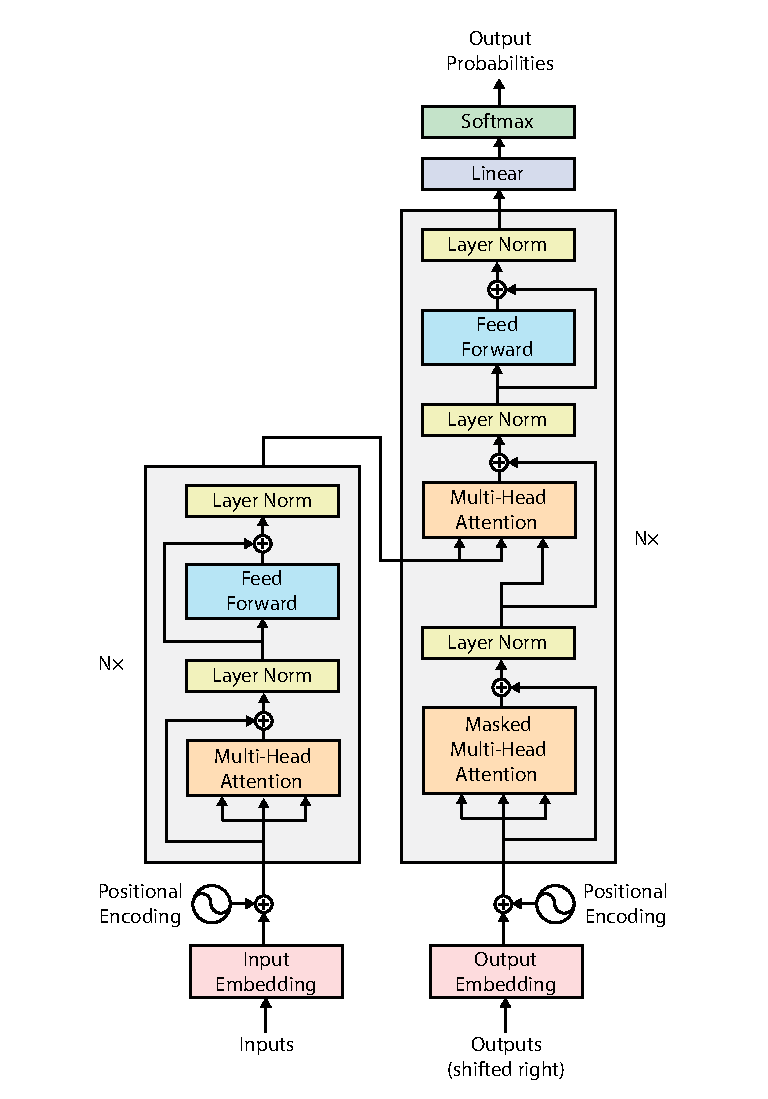
\includegraphics[width=0.8\textwidth]{figures/transformer_architecture.pdf}
    \caption{Architecture of a standard Transformer \textcite{vaswani2017attention}}
    \label{fig:transformer-architecture}
\end{figure}


\subsubsection{Tokenization}
\label{sec:tokenization}
For a Transformer to process the text input, the text is first tokenized. Tokenization is the process of breaking a sequence of text into a sequence of tokens. For example, the sentence \textit{I am a sentence.} is tokenized into the words "\textit{I}", "\textit{am}", "\textit{a}", "\textit{sentence}", and "\textit{.}". The tokenization process is usually done by a tokenizer. Specifically, the transformer uses a byte pair encoding tokenizer.

\subsubsection{Embedding and Positional Encoding}
\label{sec:embedding-and-positional-encoding}
After the input text is tokenized, the next step for the model is to understand the meaning and position of the token (word) in the sequence. This is achieved by an Embedding layer and a Positional encoding layer. The results of these two layers are combined.

Two embedding layers are used. The Input Embedding layer is fed the input sequence. The Output Embedding layer accepts the target sequence after shifting the target to the right by one position and inserting a start token at the first position. The embedding layers produce a numerical representation of the input sequence, mapping each token to an embedding vector.

\begin{figure}[htp]
    \centering
    %% Creator: Matplotlib, PGF backend
%%
%% To include the figure in your LaTeX document, write
%%   \input{<filename>.pgf}
%%
%% Make sure the required packages are loaded in your preamble
%%   \usepackage{pgf}
%%
%% and, on pdftex
%%   \usepackage[utf8]{inputenc}\DeclareUnicodeCharacter{2212}{-}
%%
%% or, on luatex and xetex
%%   \usepackage{unicode-math}
%%
%% Figures using additional raster images can only be included by \input if
%% they are in the same directory as the main LaTeX file. For loading figures
%% from other directories you can use the `import` package
%%   \usepackage{import}
%%
%% and then include the figures with
%%   \import{<path to file>}{<filename>.pgf}
%%
%% Matplotlib used the following preamble
%%
\begingroup%
\makeatletter%
\begin{pgfpicture}%
\pgfpathrectangle{\pgfpointorigin}{\pgfqpoint{4.840359in}{2.401102in}}%
\pgfusepath{use as bounding box, clip}%
\begin{pgfscope}%
\pgfsetbuttcap%
\pgfsetmiterjoin%
\definecolor{currentfill}{rgb}{1.000000,1.000000,1.000000}%
\pgfsetfillcolor{currentfill}%
\pgfsetlinewidth{0.000000pt}%
\definecolor{currentstroke}{rgb}{1.000000,1.000000,1.000000}%
\pgfsetstrokecolor{currentstroke}%
\pgfsetdash{}{0pt}%
\pgfpathmoveto{\pgfqpoint{0.000000in}{-0.000000in}}%
\pgfpathlineto{\pgfqpoint{4.840359in}{-0.000000in}}%
\pgfpathlineto{\pgfqpoint{4.840359in}{2.401102in}}%
\pgfpathlineto{\pgfqpoint{0.000000in}{2.401102in}}%
\pgfpathclose%
\pgfusepath{fill}%
\end{pgfscope}%
\begin{pgfscope}%
\pgfsetbuttcap%
\pgfsetmiterjoin%
\definecolor{currentfill}{rgb}{1.000000,1.000000,1.000000}%
\pgfsetfillcolor{currentfill}%
\pgfsetlinewidth{0.000000pt}%
\definecolor{currentstroke}{rgb}{0.000000,0.000000,0.000000}%
\pgfsetstrokecolor{currentstroke}%
\pgfsetstrokeopacity{0.000000}%
\pgfsetdash{}{0pt}%
\pgfpathmoveto{\pgfqpoint{0.584568in}{0.499691in}}%
\pgfpathlineto{\pgfqpoint{4.053193in}{0.499691in}}%
\pgfpathlineto{\pgfqpoint{4.053193in}{2.252877in}}%
\pgfpathlineto{\pgfqpoint{0.584568in}{2.252877in}}%
\pgfpathclose%
\pgfusepath{fill}%
\end{pgfscope}%
\begin{pgfscope}%
\pgfsys@transformshift{0.584167in}{0.500269in}%
\pgftext[left,bottom]{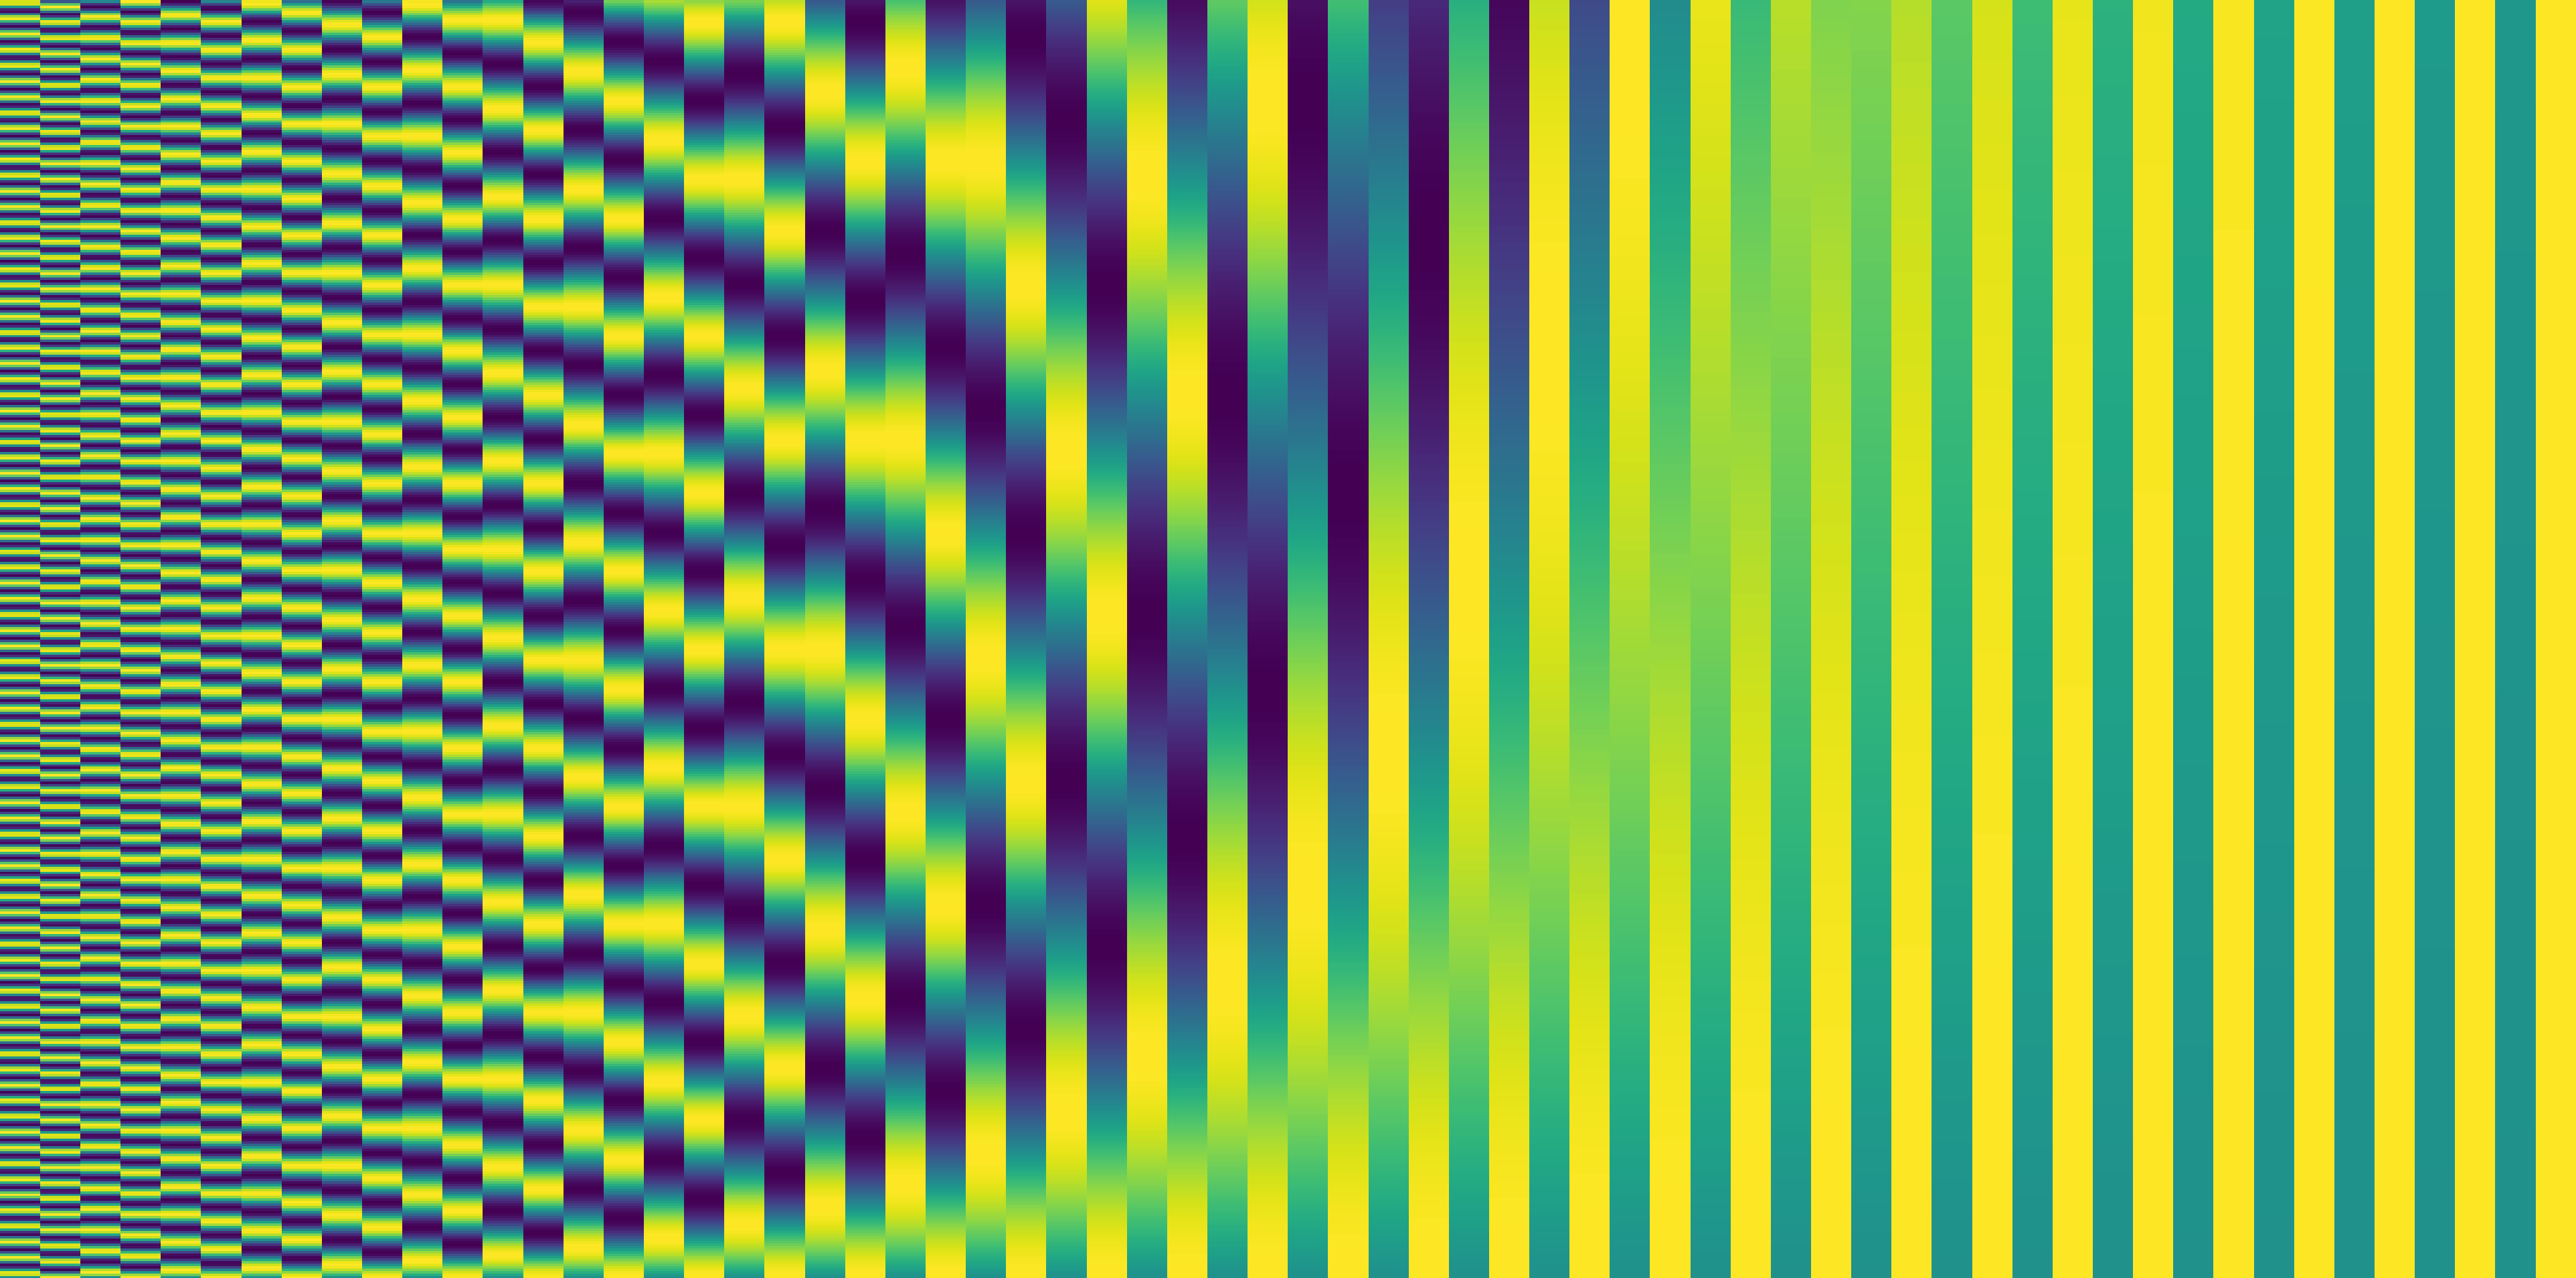
\includegraphics[interpolate=true,width=3.469167in,height=1.752500in]{figures/positional_embedding-img0.png}}%
\end{pgfscope}%
\begin{pgfscope}%
\pgfsetbuttcap%
\pgfsetroundjoin%
\definecolor{currentfill}{rgb}{0.000000,0.000000,0.000000}%
\pgfsetfillcolor{currentfill}%
\pgfsetlinewidth{0.803000pt}%
\definecolor{currentstroke}{rgb}{0.000000,0.000000,0.000000}%
\pgfsetstrokecolor{currentstroke}%
\pgfsetdash{}{0pt}%
\pgfsys@defobject{currentmarker}{\pgfqpoint{0.000000in}{-0.048611in}}{\pgfqpoint{0.000000in}{0.000000in}}{%
\pgfpathmoveto{\pgfqpoint{0.000000in}{0.000000in}}%
\pgfpathlineto{\pgfqpoint{0.000000in}{-0.048611in}}%
\pgfusepath{stroke,fill}%
}%
\begin{pgfscope}%
\pgfsys@transformshift{0.584568in}{0.499691in}%
\pgfsys@useobject{currentmarker}{}%
\end{pgfscope}%
\end{pgfscope}%
\begin{pgfscope}%
\definecolor{textcolor}{rgb}{0.000000,0.000000,0.000000}%
\pgfsetstrokecolor{textcolor}%
\pgfsetfillcolor{textcolor}%
\pgftext[x=0.584568in,y=0.402469in,,top]{\color{textcolor}\rmfamily\fontsize{10.000000}{12.000000}\selectfont \(\displaystyle {0}\)}%
\end{pgfscope}%
\begin{pgfscope}%
\pgfsetbuttcap%
\pgfsetroundjoin%
\definecolor{currentfill}{rgb}{0.000000,0.000000,0.000000}%
\pgfsetfillcolor{currentfill}%
\pgfsetlinewidth{0.803000pt}%
\definecolor{currentstroke}{rgb}{0.000000,0.000000,0.000000}%
\pgfsetstrokecolor{currentstroke}%
\pgfsetdash{}{0pt}%
\pgfsys@defobject{currentmarker}{\pgfqpoint{0.000000in}{-0.048611in}}{\pgfqpoint{0.000000in}{0.000000in}}{%
\pgfpathmoveto{\pgfqpoint{0.000000in}{0.000000in}}%
\pgfpathlineto{\pgfqpoint{0.000000in}{-0.048611in}}%
\pgfusepath{stroke,fill}%
}%
\begin{pgfscope}%
\pgfsys@transformshift{1.126541in}{0.499691in}%
\pgfsys@useobject{currentmarker}{}%
\end{pgfscope}%
\end{pgfscope}%
\begin{pgfscope}%
\definecolor{textcolor}{rgb}{0.000000,0.000000,0.000000}%
\pgfsetstrokecolor{textcolor}%
\pgfsetfillcolor{textcolor}%
\pgftext[x=1.126541in,y=0.402469in,,top]{\color{textcolor}\rmfamily\fontsize{10.000000}{12.000000}\selectfont \(\displaystyle {10}\)}%
\end{pgfscope}%
\begin{pgfscope}%
\pgfsetbuttcap%
\pgfsetroundjoin%
\definecolor{currentfill}{rgb}{0.000000,0.000000,0.000000}%
\pgfsetfillcolor{currentfill}%
\pgfsetlinewidth{0.803000pt}%
\definecolor{currentstroke}{rgb}{0.000000,0.000000,0.000000}%
\pgfsetstrokecolor{currentstroke}%
\pgfsetdash{}{0pt}%
\pgfsys@defobject{currentmarker}{\pgfqpoint{0.000000in}{-0.048611in}}{\pgfqpoint{0.000000in}{0.000000in}}{%
\pgfpathmoveto{\pgfqpoint{0.000000in}{0.000000in}}%
\pgfpathlineto{\pgfqpoint{0.000000in}{-0.048611in}}%
\pgfusepath{stroke,fill}%
}%
\begin{pgfscope}%
\pgfsys@transformshift{1.668514in}{0.499691in}%
\pgfsys@useobject{currentmarker}{}%
\end{pgfscope}%
\end{pgfscope}%
\begin{pgfscope}%
\definecolor{textcolor}{rgb}{0.000000,0.000000,0.000000}%
\pgfsetstrokecolor{textcolor}%
\pgfsetfillcolor{textcolor}%
\pgftext[x=1.668514in,y=0.402469in,,top]{\color{textcolor}\rmfamily\fontsize{10.000000}{12.000000}\selectfont \(\displaystyle {20}\)}%
\end{pgfscope}%
\begin{pgfscope}%
\pgfsetbuttcap%
\pgfsetroundjoin%
\definecolor{currentfill}{rgb}{0.000000,0.000000,0.000000}%
\pgfsetfillcolor{currentfill}%
\pgfsetlinewidth{0.803000pt}%
\definecolor{currentstroke}{rgb}{0.000000,0.000000,0.000000}%
\pgfsetstrokecolor{currentstroke}%
\pgfsetdash{}{0pt}%
\pgfsys@defobject{currentmarker}{\pgfqpoint{0.000000in}{-0.048611in}}{\pgfqpoint{0.000000in}{0.000000in}}{%
\pgfpathmoveto{\pgfqpoint{0.000000in}{0.000000in}}%
\pgfpathlineto{\pgfqpoint{0.000000in}{-0.048611in}}%
\pgfusepath{stroke,fill}%
}%
\begin{pgfscope}%
\pgfsys@transformshift{2.210486in}{0.499691in}%
\pgfsys@useobject{currentmarker}{}%
\end{pgfscope}%
\end{pgfscope}%
\begin{pgfscope}%
\definecolor{textcolor}{rgb}{0.000000,0.000000,0.000000}%
\pgfsetstrokecolor{textcolor}%
\pgfsetfillcolor{textcolor}%
\pgftext[x=2.210486in,y=0.402469in,,top]{\color{textcolor}\rmfamily\fontsize{10.000000}{12.000000}\selectfont \(\displaystyle {30}\)}%
\end{pgfscope}%
\begin{pgfscope}%
\pgfsetbuttcap%
\pgfsetroundjoin%
\definecolor{currentfill}{rgb}{0.000000,0.000000,0.000000}%
\pgfsetfillcolor{currentfill}%
\pgfsetlinewidth{0.803000pt}%
\definecolor{currentstroke}{rgb}{0.000000,0.000000,0.000000}%
\pgfsetstrokecolor{currentstroke}%
\pgfsetdash{}{0pt}%
\pgfsys@defobject{currentmarker}{\pgfqpoint{0.000000in}{-0.048611in}}{\pgfqpoint{0.000000in}{0.000000in}}{%
\pgfpathmoveto{\pgfqpoint{0.000000in}{0.000000in}}%
\pgfpathlineto{\pgfqpoint{0.000000in}{-0.048611in}}%
\pgfusepath{stroke,fill}%
}%
\begin{pgfscope}%
\pgfsys@transformshift{2.752459in}{0.499691in}%
\pgfsys@useobject{currentmarker}{}%
\end{pgfscope}%
\end{pgfscope}%
\begin{pgfscope}%
\definecolor{textcolor}{rgb}{0.000000,0.000000,0.000000}%
\pgfsetstrokecolor{textcolor}%
\pgfsetfillcolor{textcolor}%
\pgftext[x=2.752459in,y=0.402469in,,top]{\color{textcolor}\rmfamily\fontsize{10.000000}{12.000000}\selectfont \(\displaystyle {40}\)}%
\end{pgfscope}%
\begin{pgfscope}%
\pgfsetbuttcap%
\pgfsetroundjoin%
\definecolor{currentfill}{rgb}{0.000000,0.000000,0.000000}%
\pgfsetfillcolor{currentfill}%
\pgfsetlinewidth{0.803000pt}%
\definecolor{currentstroke}{rgb}{0.000000,0.000000,0.000000}%
\pgfsetstrokecolor{currentstroke}%
\pgfsetdash{}{0pt}%
\pgfsys@defobject{currentmarker}{\pgfqpoint{0.000000in}{-0.048611in}}{\pgfqpoint{0.000000in}{0.000000in}}{%
\pgfpathmoveto{\pgfqpoint{0.000000in}{0.000000in}}%
\pgfpathlineto{\pgfqpoint{0.000000in}{-0.048611in}}%
\pgfusepath{stroke,fill}%
}%
\begin{pgfscope}%
\pgfsys@transformshift{3.294432in}{0.499691in}%
\pgfsys@useobject{currentmarker}{}%
\end{pgfscope}%
\end{pgfscope}%
\begin{pgfscope}%
\definecolor{textcolor}{rgb}{0.000000,0.000000,0.000000}%
\pgfsetstrokecolor{textcolor}%
\pgfsetfillcolor{textcolor}%
\pgftext[x=3.294432in,y=0.402469in,,top]{\color{textcolor}\rmfamily\fontsize{10.000000}{12.000000}\selectfont \(\displaystyle {50}\)}%
\end{pgfscope}%
\begin{pgfscope}%
\pgfsetbuttcap%
\pgfsetroundjoin%
\definecolor{currentfill}{rgb}{0.000000,0.000000,0.000000}%
\pgfsetfillcolor{currentfill}%
\pgfsetlinewidth{0.803000pt}%
\definecolor{currentstroke}{rgb}{0.000000,0.000000,0.000000}%
\pgfsetstrokecolor{currentstroke}%
\pgfsetdash{}{0pt}%
\pgfsys@defobject{currentmarker}{\pgfqpoint{0.000000in}{-0.048611in}}{\pgfqpoint{0.000000in}{0.000000in}}{%
\pgfpathmoveto{\pgfqpoint{0.000000in}{0.000000in}}%
\pgfpathlineto{\pgfqpoint{0.000000in}{-0.048611in}}%
\pgfusepath{stroke,fill}%
}%
\begin{pgfscope}%
\pgfsys@transformshift{3.836404in}{0.499691in}%
\pgfsys@useobject{currentmarker}{}%
\end{pgfscope}%
\end{pgfscope}%
\begin{pgfscope}%
\definecolor{textcolor}{rgb}{0.000000,0.000000,0.000000}%
\pgfsetstrokecolor{textcolor}%
\pgfsetfillcolor{textcolor}%
\pgftext[x=3.836404in,y=0.402469in,,top]{\color{textcolor}\rmfamily\fontsize{10.000000}{12.000000}\selectfont \(\displaystyle {60}\)}%
\end{pgfscope}%
\begin{pgfscope}%
\definecolor{textcolor}{rgb}{0.000000,0.000000,0.000000}%
\pgfsetstrokecolor{textcolor}%
\pgfsetfillcolor{textcolor}%
\pgftext[x=2.318881in,y=0.223457in,,top]{\color{textcolor}\rmfamily\fontsize{10.000000}{12.000000}\selectfont Depth}%
\end{pgfscope}%
\begin{pgfscope}%
\pgfsetbuttcap%
\pgfsetroundjoin%
\definecolor{currentfill}{rgb}{0.000000,0.000000,0.000000}%
\pgfsetfillcolor{currentfill}%
\pgfsetlinewidth{0.803000pt}%
\definecolor{currentstroke}{rgb}{0.000000,0.000000,0.000000}%
\pgfsetstrokecolor{currentstroke}%
\pgfsetdash{}{0pt}%
\pgfsys@defobject{currentmarker}{\pgfqpoint{-0.048611in}{0.000000in}}{\pgfqpoint{0.000000in}{0.000000in}}{%
\pgfpathmoveto{\pgfqpoint{0.000000in}{0.000000in}}%
\pgfpathlineto{\pgfqpoint{-0.048611in}{0.000000in}}%
\pgfusepath{stroke,fill}%
}%
\begin{pgfscope}%
\pgfsys@transformshift{0.584568in}{0.499691in}%
\pgfsys@useobject{currentmarker}{}%
\end{pgfscope}%
\end{pgfscope}%
\begin{pgfscope}%
\definecolor{textcolor}{rgb}{0.000000,0.000000,0.000000}%
\pgfsetstrokecolor{textcolor}%
\pgfsetfillcolor{textcolor}%
\pgftext[x=0.417902in, y=0.451466in, left, base]{\color{textcolor}\rmfamily\fontsize{10.000000}{12.000000}\selectfont \(\displaystyle {0}\)}%
\end{pgfscope}%
\begin{pgfscope}%
\pgfsetbuttcap%
\pgfsetroundjoin%
\definecolor{currentfill}{rgb}{0.000000,0.000000,0.000000}%
\pgfsetfillcolor{currentfill}%
\pgfsetlinewidth{0.803000pt}%
\definecolor{currentstroke}{rgb}{0.000000,0.000000,0.000000}%
\pgfsetstrokecolor{currentstroke}%
\pgfsetdash{}{0pt}%
\pgfsys@defobject{currentmarker}{\pgfqpoint{-0.048611in}{0.000000in}}{\pgfqpoint{0.000000in}{0.000000in}}{%
\pgfpathmoveto{\pgfqpoint{0.000000in}{0.000000in}}%
\pgfpathlineto{\pgfqpoint{-0.048611in}{0.000000in}}%
\pgfusepath{stroke,fill}%
}%
\begin{pgfscope}%
\pgfsys@transformshift{0.584568in}{0.842110in}%
\pgfsys@useobject{currentmarker}{}%
\end{pgfscope}%
\end{pgfscope}%
\begin{pgfscope}%
\definecolor{textcolor}{rgb}{0.000000,0.000000,0.000000}%
\pgfsetstrokecolor{textcolor}%
\pgfsetfillcolor{textcolor}%
\pgftext[x=0.279012in, y=0.793885in, left, base]{\color{textcolor}\rmfamily\fontsize{10.000000}{12.000000}\selectfont \(\displaystyle {100}\)}%
\end{pgfscope}%
\begin{pgfscope}%
\pgfsetbuttcap%
\pgfsetroundjoin%
\definecolor{currentfill}{rgb}{0.000000,0.000000,0.000000}%
\pgfsetfillcolor{currentfill}%
\pgfsetlinewidth{0.803000pt}%
\definecolor{currentstroke}{rgb}{0.000000,0.000000,0.000000}%
\pgfsetstrokecolor{currentstroke}%
\pgfsetdash{}{0pt}%
\pgfsys@defobject{currentmarker}{\pgfqpoint{-0.048611in}{0.000000in}}{\pgfqpoint{0.000000in}{0.000000in}}{%
\pgfpathmoveto{\pgfqpoint{0.000000in}{0.000000in}}%
\pgfpathlineto{\pgfqpoint{-0.048611in}{0.000000in}}%
\pgfusepath{stroke,fill}%
}%
\begin{pgfscope}%
\pgfsys@transformshift{0.584568in}{1.184529in}%
\pgfsys@useobject{currentmarker}{}%
\end{pgfscope}%
\end{pgfscope}%
\begin{pgfscope}%
\definecolor{textcolor}{rgb}{0.000000,0.000000,0.000000}%
\pgfsetstrokecolor{textcolor}%
\pgfsetfillcolor{textcolor}%
\pgftext[x=0.279012in, y=1.136304in, left, base]{\color{textcolor}\rmfamily\fontsize{10.000000}{12.000000}\selectfont \(\displaystyle {200}\)}%
\end{pgfscope}%
\begin{pgfscope}%
\pgfsetbuttcap%
\pgfsetroundjoin%
\definecolor{currentfill}{rgb}{0.000000,0.000000,0.000000}%
\pgfsetfillcolor{currentfill}%
\pgfsetlinewidth{0.803000pt}%
\definecolor{currentstroke}{rgb}{0.000000,0.000000,0.000000}%
\pgfsetstrokecolor{currentstroke}%
\pgfsetdash{}{0pt}%
\pgfsys@defobject{currentmarker}{\pgfqpoint{-0.048611in}{0.000000in}}{\pgfqpoint{0.000000in}{0.000000in}}{%
\pgfpathmoveto{\pgfqpoint{0.000000in}{0.000000in}}%
\pgfpathlineto{\pgfqpoint{-0.048611in}{0.000000in}}%
\pgfusepath{stroke,fill}%
}%
\begin{pgfscope}%
\pgfsys@transformshift{0.584568in}{1.526949in}%
\pgfsys@useobject{currentmarker}{}%
\end{pgfscope}%
\end{pgfscope}%
\begin{pgfscope}%
\definecolor{textcolor}{rgb}{0.000000,0.000000,0.000000}%
\pgfsetstrokecolor{textcolor}%
\pgfsetfillcolor{textcolor}%
\pgftext[x=0.279012in, y=1.478723in, left, base]{\color{textcolor}\rmfamily\fontsize{10.000000}{12.000000}\selectfont \(\displaystyle {300}\)}%
\end{pgfscope}%
\begin{pgfscope}%
\pgfsetbuttcap%
\pgfsetroundjoin%
\definecolor{currentfill}{rgb}{0.000000,0.000000,0.000000}%
\pgfsetfillcolor{currentfill}%
\pgfsetlinewidth{0.803000pt}%
\definecolor{currentstroke}{rgb}{0.000000,0.000000,0.000000}%
\pgfsetstrokecolor{currentstroke}%
\pgfsetdash{}{0pt}%
\pgfsys@defobject{currentmarker}{\pgfqpoint{-0.048611in}{0.000000in}}{\pgfqpoint{0.000000in}{0.000000in}}{%
\pgfpathmoveto{\pgfqpoint{0.000000in}{0.000000in}}%
\pgfpathlineto{\pgfqpoint{-0.048611in}{0.000000in}}%
\pgfusepath{stroke,fill}%
}%
\begin{pgfscope}%
\pgfsys@transformshift{0.584568in}{1.869368in}%
\pgfsys@useobject{currentmarker}{}%
\end{pgfscope}%
\end{pgfscope}%
\begin{pgfscope}%
\definecolor{textcolor}{rgb}{0.000000,0.000000,0.000000}%
\pgfsetstrokecolor{textcolor}%
\pgfsetfillcolor{textcolor}%
\pgftext[x=0.279012in, y=1.821142in, left, base]{\color{textcolor}\rmfamily\fontsize{10.000000}{12.000000}\selectfont \(\displaystyle {400}\)}%
\end{pgfscope}%
\begin{pgfscope}%
\pgfsetbuttcap%
\pgfsetroundjoin%
\definecolor{currentfill}{rgb}{0.000000,0.000000,0.000000}%
\pgfsetfillcolor{currentfill}%
\pgfsetlinewidth{0.803000pt}%
\definecolor{currentstroke}{rgb}{0.000000,0.000000,0.000000}%
\pgfsetstrokecolor{currentstroke}%
\pgfsetdash{}{0pt}%
\pgfsys@defobject{currentmarker}{\pgfqpoint{-0.048611in}{0.000000in}}{\pgfqpoint{0.000000in}{0.000000in}}{%
\pgfpathmoveto{\pgfqpoint{0.000000in}{0.000000in}}%
\pgfpathlineto{\pgfqpoint{-0.048611in}{0.000000in}}%
\pgfusepath{stroke,fill}%
}%
\begin{pgfscope}%
\pgfsys@transformshift{0.584568in}{2.211787in}%
\pgfsys@useobject{currentmarker}{}%
\end{pgfscope}%
\end{pgfscope}%
\begin{pgfscope}%
\definecolor{textcolor}{rgb}{0.000000,0.000000,0.000000}%
\pgfsetstrokecolor{textcolor}%
\pgfsetfillcolor{textcolor}%
\pgftext[x=0.279012in, y=2.163562in, left, base]{\color{textcolor}\rmfamily\fontsize{10.000000}{12.000000}\selectfont \(\displaystyle {500}\)}%
\end{pgfscope}%
\begin{pgfscope}%
\definecolor{textcolor}{rgb}{0.000000,0.000000,0.000000}%
\pgfsetstrokecolor{textcolor}%
\pgfsetfillcolor{textcolor}%
\pgftext[x=0.223457in,y=1.376284in,,bottom,rotate=90.000000]{\color{textcolor}\rmfamily\fontsize{10.000000}{12.000000}\selectfont Position}%
\end{pgfscope}%
\begin{pgfscope}%
\pgfsetrectcap%
\pgfsetmiterjoin%
\pgfsetlinewidth{0.803000pt}%
\definecolor{currentstroke}{rgb}{0.000000,0.000000,0.000000}%
\pgfsetstrokecolor{currentstroke}%
\pgfsetdash{}{0pt}%
\pgfpathmoveto{\pgfqpoint{0.584568in}{0.499691in}}%
\pgfpathlineto{\pgfqpoint{0.584568in}{2.252877in}}%
\pgfusepath{stroke}%
\end{pgfscope}%
\begin{pgfscope}%
\pgfsetrectcap%
\pgfsetmiterjoin%
\pgfsetlinewidth{0.803000pt}%
\definecolor{currentstroke}{rgb}{0.000000,0.000000,0.000000}%
\pgfsetstrokecolor{currentstroke}%
\pgfsetdash{}{0pt}%
\pgfpathmoveto{\pgfqpoint{4.053193in}{0.499691in}}%
\pgfpathlineto{\pgfqpoint{4.053193in}{2.252877in}}%
\pgfusepath{stroke}%
\end{pgfscope}%
\begin{pgfscope}%
\pgfsetrectcap%
\pgfsetmiterjoin%
\pgfsetlinewidth{0.803000pt}%
\definecolor{currentstroke}{rgb}{0.000000,0.000000,0.000000}%
\pgfsetstrokecolor{currentstroke}%
\pgfsetdash{}{0pt}%
\pgfpathmoveto{\pgfqpoint{0.584568in}{0.499691in}}%
\pgfpathlineto{\pgfqpoint{4.053193in}{0.499691in}}%
\pgfusepath{stroke}%
\end{pgfscope}%
\begin{pgfscope}%
\pgfsetrectcap%
\pgfsetmiterjoin%
\pgfsetlinewidth{0.803000pt}%
\definecolor{currentstroke}{rgb}{0.000000,0.000000,0.000000}%
\pgfsetstrokecolor{currentstroke}%
\pgfsetdash{}{0pt}%
\pgfpathmoveto{\pgfqpoint{0.584568in}{2.252877in}}%
\pgfpathlineto{\pgfqpoint{4.053193in}{2.252877in}}%
\pgfusepath{stroke}%
\end{pgfscope}%
\begin{pgfscope}%
\pgfpathrectangle{\pgfqpoint{4.269982in}{0.499691in}}{\pgfqpoint{0.087659in}{1.753186in}}%
\pgfusepath{clip}%
\pgfsetbuttcap%
\pgfsetmiterjoin%
\definecolor{currentfill}{rgb}{1.000000,1.000000,1.000000}%
\pgfsetfillcolor{currentfill}%
\pgfsetlinewidth{0.010037pt}%
\definecolor{currentstroke}{rgb}{1.000000,1.000000,1.000000}%
\pgfsetstrokecolor{currentstroke}%
\pgfsetdash{}{0pt}%
\pgfpathmoveto{\pgfqpoint{4.269982in}{0.499691in}}%
\pgfpathlineto{\pgfqpoint{4.269982in}{0.506539in}}%
\pgfpathlineto{\pgfqpoint{4.269982in}{2.246029in}}%
\pgfpathlineto{\pgfqpoint{4.269982in}{2.252877in}}%
\pgfpathlineto{\pgfqpoint{4.357642in}{2.252877in}}%
\pgfpathlineto{\pgfqpoint{4.357642in}{2.246029in}}%
\pgfpathlineto{\pgfqpoint{4.357642in}{0.506539in}}%
\pgfpathlineto{\pgfqpoint{4.357642in}{0.499691in}}%
\pgfpathclose%
\pgfusepath{stroke,fill}%
\end{pgfscope}%
\begin{pgfscope}%
\pgfsys@transformshift{4.270000in}{0.500269in}%
\pgftext[left,bottom]{
\includegraphics[interpolate=true,width=0.087500in,height=1.752500in]{figures/positional_embedding-img1.png}}%
\end{pgfscope}%
\begin{pgfscope}%
\pgfsetbuttcap%
\pgfsetroundjoin%
\definecolor{currentfill}{rgb}{0.000000,0.000000,0.000000}%
\pgfsetfillcolor{currentfill}%
\pgfsetlinewidth{0.803000pt}%
\definecolor{currentstroke}{rgb}{0.000000,0.000000,0.000000}%
\pgfsetstrokecolor{currentstroke}%
\pgfsetdash{}{0pt}%
\pgfsys@defobject{currentmarker}{\pgfqpoint{0.000000in}{0.000000in}}{\pgfqpoint{0.048611in}{0.000000in}}{%
\pgfpathmoveto{\pgfqpoint{0.000000in}{0.000000in}}%
\pgfpathlineto{\pgfqpoint{0.048611in}{0.000000in}}%
\pgfusepath{stroke,fill}%
}%
\begin{pgfscope}%
\pgfsys@transformshift{4.357642in}{0.499691in}%
\pgfsys@useobject{currentmarker}{}%
\end{pgfscope}%
\end{pgfscope}%
\begin{pgfscope}%
\definecolor{textcolor}{rgb}{0.000000,0.000000,0.000000}%
\pgfsetstrokecolor{textcolor}%
\pgfsetfillcolor{textcolor}%
\pgftext[x=4.454864in, y=0.451466in, left, base]{\color{textcolor}\rmfamily\fontsize{10.000000}{12.000000}\selectfont \(\displaystyle {-1.0}\)}%
\end{pgfscope}%
\begin{pgfscope}%
\pgfsetbuttcap%
\pgfsetroundjoin%
\definecolor{currentfill}{rgb}{0.000000,0.000000,0.000000}%
\pgfsetfillcolor{currentfill}%
\pgfsetlinewidth{0.803000pt}%
\definecolor{currentstroke}{rgb}{0.000000,0.000000,0.000000}%
\pgfsetstrokecolor{currentstroke}%
\pgfsetdash{}{0pt}%
\pgfsys@defobject{currentmarker}{\pgfqpoint{0.000000in}{0.000000in}}{\pgfqpoint{0.048611in}{0.000000in}}{%
\pgfpathmoveto{\pgfqpoint{0.000000in}{0.000000in}}%
\pgfpathlineto{\pgfqpoint{0.048611in}{0.000000in}}%
\pgfusepath{stroke,fill}%
}%
\begin{pgfscope}%
\pgfsys@transformshift{4.357642in}{0.937988in}%
\pgfsys@useobject{currentmarker}{}%
\end{pgfscope}%
\end{pgfscope}%
\begin{pgfscope}%
\definecolor{textcolor}{rgb}{0.000000,0.000000,0.000000}%
\pgfsetstrokecolor{textcolor}%
\pgfsetfillcolor{textcolor}%
\pgftext[x=4.454864in, y=0.889762in, left, base]{\color{textcolor}\rmfamily\fontsize{10.000000}{12.000000}\selectfont \(\displaystyle {-0.5}\)}%
\end{pgfscope}%
\begin{pgfscope}%
\pgfsetbuttcap%
\pgfsetroundjoin%
\definecolor{currentfill}{rgb}{0.000000,0.000000,0.000000}%
\pgfsetfillcolor{currentfill}%
\pgfsetlinewidth{0.803000pt}%
\definecolor{currentstroke}{rgb}{0.000000,0.000000,0.000000}%
\pgfsetstrokecolor{currentstroke}%
\pgfsetdash{}{0pt}%
\pgfsys@defobject{currentmarker}{\pgfqpoint{0.000000in}{0.000000in}}{\pgfqpoint{0.048611in}{0.000000in}}{%
\pgfpathmoveto{\pgfqpoint{0.000000in}{0.000000in}}%
\pgfpathlineto{\pgfqpoint{0.048611in}{0.000000in}}%
\pgfusepath{stroke,fill}%
}%
\begin{pgfscope}%
\pgfsys@transformshift{4.357642in}{1.376284in}%
\pgfsys@useobject{currentmarker}{}%
\end{pgfscope}%
\end{pgfscope}%
\begin{pgfscope}%
\definecolor{textcolor}{rgb}{0.000000,0.000000,0.000000}%
\pgfsetstrokecolor{textcolor}%
\pgfsetfillcolor{textcolor}%
\pgftext[x=4.454864in, y=1.328059in, left, base]{\color{textcolor}\rmfamily\fontsize{10.000000}{12.000000}\selectfont \(\displaystyle {0.0}\)}%
\end{pgfscope}%
\begin{pgfscope}%
\pgfsetbuttcap%
\pgfsetroundjoin%
\definecolor{currentfill}{rgb}{0.000000,0.000000,0.000000}%
\pgfsetfillcolor{currentfill}%
\pgfsetlinewidth{0.803000pt}%
\definecolor{currentstroke}{rgb}{0.000000,0.000000,0.000000}%
\pgfsetstrokecolor{currentstroke}%
\pgfsetdash{}{0pt}%
\pgfsys@defobject{currentmarker}{\pgfqpoint{0.000000in}{0.000000in}}{\pgfqpoint{0.048611in}{0.000000in}}{%
\pgfpathmoveto{\pgfqpoint{0.000000in}{0.000000in}}%
\pgfpathlineto{\pgfqpoint{0.048611in}{0.000000in}}%
\pgfusepath{stroke,fill}%
}%
\begin{pgfscope}%
\pgfsys@transformshift{4.357642in}{1.814581in}%
\pgfsys@useobject{currentmarker}{}%
\end{pgfscope}%
\end{pgfscope}%
\begin{pgfscope}%
\definecolor{textcolor}{rgb}{0.000000,0.000000,0.000000}%
\pgfsetstrokecolor{textcolor}%
\pgfsetfillcolor{textcolor}%
\pgftext[x=4.454864in, y=1.766355in, left, base]{\color{textcolor}\rmfamily\fontsize{10.000000}{12.000000}\selectfont \(\displaystyle {0.5}\)}%
\end{pgfscope}%
\begin{pgfscope}%
\pgfsetbuttcap%
\pgfsetroundjoin%
\definecolor{currentfill}{rgb}{0.000000,0.000000,0.000000}%
\pgfsetfillcolor{currentfill}%
\pgfsetlinewidth{0.803000pt}%
\definecolor{currentstroke}{rgb}{0.000000,0.000000,0.000000}%
\pgfsetstrokecolor{currentstroke}%
\pgfsetdash{}{0pt}%
\pgfsys@defobject{currentmarker}{\pgfqpoint{0.000000in}{0.000000in}}{\pgfqpoint{0.048611in}{0.000000in}}{%
\pgfpathmoveto{\pgfqpoint{0.000000in}{0.000000in}}%
\pgfpathlineto{\pgfqpoint{0.048611in}{0.000000in}}%
\pgfusepath{stroke,fill}%
}%
\begin{pgfscope}%
\pgfsys@transformshift{4.357642in}{2.252877in}%
\pgfsys@useobject{currentmarker}{}%
\end{pgfscope}%
\end{pgfscope}%
\begin{pgfscope}%
\definecolor{textcolor}{rgb}{0.000000,0.000000,0.000000}%
\pgfsetstrokecolor{textcolor}%
\pgfsetfillcolor{textcolor}%
\pgftext[x=4.454864in, y=2.204652in, left, base]{\color{textcolor}\rmfamily\fontsize{10.000000}{12.000000}\selectfont \(\displaystyle {1.0}\)}%
\end{pgfscope}%
\begin{pgfscope}%
\pgfsetbuttcap%
\pgfsetmiterjoin%
\pgfsetlinewidth{0.803000pt}%
\definecolor{currentstroke}{rgb}{0.000000,0.000000,0.000000}%
\pgfsetstrokecolor{currentstroke}%
\pgfsetdash{}{0pt}%
\pgfpathmoveto{\pgfqpoint{4.269982in}{0.499691in}}%
\pgfpathlineto{\pgfqpoint{4.269982in}{0.506539in}}%
\pgfpathlineto{\pgfqpoint{4.269982in}{2.246029in}}%
\pgfpathlineto{\pgfqpoint{4.269982in}{2.252877in}}%
\pgfpathlineto{\pgfqpoint{4.357642in}{2.252877in}}%
\pgfpathlineto{\pgfqpoint{4.357642in}{2.246029in}}%
\pgfpathlineto{\pgfqpoint{4.357642in}{0.506539in}}%
\pgfpathlineto{\pgfqpoint{4.357642in}{0.499691in}}%
\pgfpathclose%
\pgfusepath{stroke}%
\end{pgfscope}%
\end{pgfpicture}%
\makeatother%
\endgroup%

    \caption{The 64-dimensional positional encoding for a sentence with the maximum length of 512. Each row represents an positional encoding vector.}
    \label{fig:positional-embedding}
\end{figure}

The positional encoding is generated by a sinusoidal positional encoding layer. This layer is fed the sequence length and produces a sinusoidal positional encoding vector. This is illustrated in \cref{fig:positional-embedding}, where each row corresponds to one sinusoidal positional encoding vector. The positional encoding vector is then added to the embedding vector.

\subsubsection{Encoder and decoder stacks}
\label{sec:encoder-decoder-stacks}
A Transformer is comprised of two main parts: the encoder and the decoder. The encoder is responsible for encoding the input sequence into a sequence of vectors. It tries to capture information about which parts of the inputs are relevant to each other. The decoder is responsible for decoding the output sequence from the encoder. Along with other inputs, the decoder is optimized for generating outputs. In \cref{fig:transformer-architecture}, the left and right halves represent the Transformer encoder and decoder, respectively. 

The encoder and decoder are both composed of a stack of self-attention layers. This layer allows the model to pay more or less attention to certain words in the input sentence as it is handling a specific word. Each decoder layer has an additional attention mechanism that draws information from the outputs of previous decoders, before the decoder layer draws information from the encodings. Both the encoder and decoder layers contain a feed-forward layer for further processing of the outputs, as well as layer normalization and residual connections.

The transformer architecture allows for auto-regressive text generation. This is achieved by re-feeding the decoder the encoder outputs. The decoder then generates the next word in a loop until the end of the sentence is reached. For this to work, the  Transformer must not be able to use the current or future output to predict an output. The use of a look-ahead mask solves this. The final output from the transformer is generated by feeding the decoder output through a linear layer and a softmax layer. This produces probabilities for each token in the vocabulary and can be used to predict the next token (word).

The encoder and decoder can also be used independently or in combination. The original transformer model described by \textcite{vaswani2017attention} used an encoder-decoder structure. These models are used for generative tasks that also require input, for example, language translation or text summarization. Encoder-only models are used for tasks that are centered around understanding the input, such as sentence classification and named entity recognition. Decoder-only models excel at generative tasks such as text generation.

\begin{figure}[htp]
    \centering
    \begin{subfigure}[b]{0.5\textwidth}
        \centering
        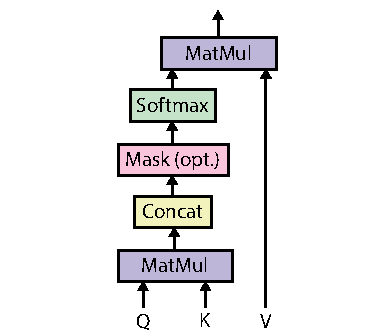
\includegraphics[width=0.8\textwidth,keepaspectratio]{figures/scaled_dot-product_attention.pdf}
        \caption{Scaled Dot-Product Attention.}
        \label{fig:scaled-dotproduct-attention}
    \end{subfigure}%
    \hfill
    \begin{subfigure}[b]{0.5\textwidth}
        \centering
        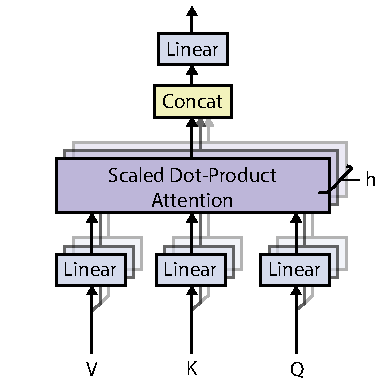
\includegraphics[width=0.8\textwidth,keepaspectratio]{figures/multi-head_attention.pdf}
        \caption{Multi-Head Attention consists of several attention layers running in parallel.}
        \label{fig:multihead-attention}
    \end{subfigure}%
    \caption{Multi-Head Attention module in Transformer architecture \textcite{vaswani2017attention}}
    \label{fig:transformer-architecture-details}
\end{figure}

\subsubsection{Scaled dot-product attention} 
\label{sec:scaled-dot-product-attention}
The self-attention layer used in each Transformer block is named "Scaled Dot-Product Attention". An overview of the attention layer is shown in \cref{fig:scaled-dotproduct-attention}. The layer learns three weight matrices, query weights \(W_Q\), key weights \(W_K\), and value weights \(W_V\). Each input word embedding is multiplied with each weight matrix, producing a query vector, key vector, and value vector. Self-attention scores are then generated by calculating the dot products of the query vector with the key vector of the respective word (query) that is calculated.

In order to stabilize the gradients during training, the attention weights are divided by the square root of the dimension of the key vectors, \(\sqrt{d_{k}}\). A softmax function is then applied, normalizing the scores to be positive and adding up to 1. Each value vector is then multiplied by the softmax score. The resulting weighted value vectors are then summed up and serve as output from the attention layer.

In practice, the attention calculation for all tokens can be expressed as one large matrix calculation, as shown in \cref{fig:scaled-dotproduct-attention}. This significantly speeds up the training process. The queries, keys, and values are packed into the separate matrices \(Q\), \(K\), and \(V\), respectively. The output matrix can be described as:
\begin{equation}
    \text{Attention$(Q,K,V)$} = \text{softmax}(\frac{QK^T}{\sqrt{d_{k}}})V
\end{equation}
where the superscript \(T\) represent the transpose operation.

\subsubsection{Multi-head attention}
\label{sec:multi-head-attention}
By splitting the query, key, and value parameters in N-ways (logically), each with its separate weight matrix, the performance of the Transformer is increased. This is called multi-head attention, illustrated in \cref{fig:multihead-attention}. It gives the Transformer greater power to encode multiple relationships and nuances for each word. The final attention outputs for the feed-forward network are calculated by concatenating the matrixes for each attention head.

\subsection{Training}
\label{sec:transformer-training}
A Transformer model typically undergoes something called self-supervised learning. This is an intermediary between both unsupervised- and supervised learning. This normally conforms to unsupervised pre-training the model on a large set of data. Then, the model is fine-tuned on a (usually) smaller dataset of labeled data.

In contrast to the unsupervised training, where the target sequence comprises the predicted transformer output, the supervised training is done by feeding the complete input- and target language sequence directly into the Transformer. The input sequence is fed to the encoder, while the target sequence is fed to the decoder.

\subsection{Inference}
\label{sec:transformer-inference}
For making inference, the Transformer is only fed the input sequence. The encoder is run on the input sequence, and the encoder output is fed to the decoder. Since no encoder output is available at the first timestep, the decoder is fed a special "<start>" token. The decoder output is then fed back into the decoder again. This process is repeated until the decoder output encounters a special "<stop>" token.

\section{Relevant Metrics}
\label{sec:metrics}

\subsection{Machine learning performance metric}
\label{sec:performance-metric}

\subsubsection{Accuracy}
\label{sec:accuracy}
Accuracy is the proportion of correct predictions among the total number of cases processed \cite{accuracy}. Accuracy is formally defined as the proportion of correct predictions among the total number of cases processed, as seen in \cref{eq:accuracy}.

\begin{equation}
    \label{eq:accuracy}
    \text{Accuracy} = \frac{TP + TN}{TP + TN + FP + FN}
\end{equation}
where \(TP\) is the number of true positives, \(TN\) is the number of true negatives, \(FP\) is the number of false positives, and \(FN\) is the number of false negatives.

It is a very common metric used for evaluating the performance of a machine learning model. However, it has to be used with caution, as an overfitted model would report high accuracy.

\subsubsection{Perplexity}
\label{sec:perplexity}
Perplexity is one of the most common metrics for evaluating language models \cite{perplexity}. It is a measure of how variable a prediction model is, and can be defined as the normalized inverse probability of the test set \cite{perplexity2}. For a test set with words \(W  = w_1, w_2, …, w_N\), the perplexity of the model on the test set is:

\begin{equation}
    \label{eq:perplexity}
    PP(W) = \sqrt[N]{\frac{1}{p(w_1,w_2,...,w_N)}}
\end{equation}

Perplexity can be interpreted as the weighted branching factor. If we have a perplexity of 10, it means that whenever the model tries to guess the next word, it is as confused as if it had to pick between 10 words. Models with lower perplexity have probability values that are more varied. Meaning, the lower perplexity, the better model \cite{perplexity2}.

\subsection{Machine translation performance metrics}
\label{sec:machine-translation-metrics}

\subsubsection{\textsc{Bleu}}
\label{sec:blue-score}
\acrfullr{bleu} by \textcite{papineni2002bleu} is a metric for automatically evaluating machine-translated text. \acrshort{bleu} scores are between 0 and 1. A value of 0 means there is no overlap with the reference translation, while a value of 1 means that the translation perfectly overlaps. A score of 0.6 or 0.7 is considered the best a human can achieve \cite{googlebleu,papineni2002bleu}. The color gradient in \cref{fig:bleu} from \cite{lavie2011evaluating} can be used as a general scale interpretation of the BLEU score.

\begin{figure}
    \centering
    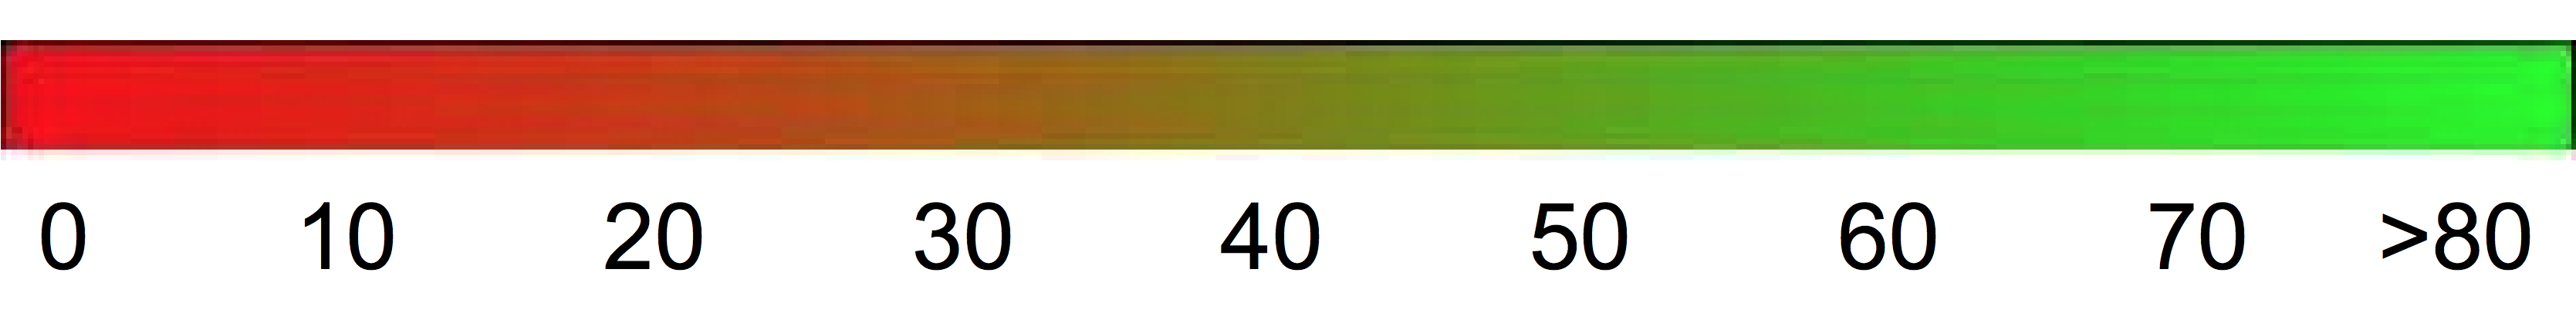
\includegraphics[width=\textwidth,keepaspectratio]{figures/bleu_score_range.png}
    \caption{Gradient for interpreting BLEU score \textcite{lavie2011evaluating}.}
    \label{fig:bleu}
\end{figure}
The method is based on n-gram matching, where n-grams in the reference translation are matched against n-grams in the translation. The matches are position-independent. The more matches, the higher the score.\\

\noindent For example, consider the following two translations:\\

\indent Candidate: \underline{on} \underline{the} \underline{mat} \underline{the} \underline{cat} sat.\\
\indent Reference: \underline{The} \underline{cat} is \underline{on} \underline{the} \underline{mat}.\\

\noindent The unigram precision \(\left(p_1\right) = 5/6\)\\

\noindent However, machine translations tend to generate an abundance of reasonable words, which could result in an inaccurately high precision. To combat this, \acrshort{bleu} uses something called modified precision\cite{papineni2002bleu}. The modification consists of clipping the occurrence of an n-gram to the maximum number the n-gram occurs in the reference. These clipped precision scores \(\left(p_n\right)\) are then calculated for n-grams up to length \(N\), normally 1-grams through 4-grams. They are then combined by computing the geometric average precision, as shown in \cref{eq:geometric-average-precision}. In addition, positive weights \(w_n\) are used, normally set to \(w_n = 1/N\).

\begin{equation}
    \label{eq:geometric-average-precision}
    \text{Geometric Average Precision $\left(N\right)$} = \exp \left( \sum_{n=1}^{N} w_n \log{p_n} \right)
\end{equation}

\noindent \acrshort{bleu} also introduces a brevity penalty for penalizing translations that are shorter than the reference:

\begin{equation}
    \label{eqn:brevity-penalty}
    \text{Brevity Penalty} = 
    \begin{cases}
        1 & \text{if } c > r\\
        e^{\left(1-r/c \right)} & \text{if } c \le r
    \end{cases}
\end{equation}

\noindent The final \acrshort{bleu} score is then computed as:

\begin{equation}
    \label{eqn:bleu}
    \textsc{Bleu} = \text{Brevity Penalty} \cdot \text{Geometric Average Precision Scores $\left(N\right)$}
\end{equation}

\subsection{String metric}
\label{sec:string-metric}

\subsubsection{Jaccard index}
\label{sec:jaccard-index}
The Jaccard index \cite{jaccard} is also known as the Jaccard similarity coefficient. It is a statistic used for gauging the similarity of sample sets. It is defined as the size of the intersection divided by the size of the union of the sets, as shown in \cref{eqn:jaccard}.

\begin{equation}
    \label{eqn:jaccard}
    J(A,B)=\frac{|A \cap B|}{|A \cup  B|}
\end{equation}

The Jaccard index ranges from 0 to 1. The higher the number, the more similar the two sets are.

The Jaccard index can for example be used as a measure of how similar two text strings are. For this, the strings are simply converted into sets of n-grams. The n-grams are then compared using the Jaccard index.

\section{Blockchain}
\label{sec:blockchain}
Blockchain technology was popularized by Satoshi Nakamoto in 2008 with his publication of the article "Bitcoin: A Peer-to-Peer Electronic Cash System". He introduced the formal idea of a peer-to-peer electronic cash system based on blockchain. This made it possible for users to conduct transactions without any need for a central authority. A blockchain is a growing list of records linked together with the help of a cryptographic hash. Each of these records is called a block. The blocks contain a cryptographic hash of the previous block, transactional data, and a timestamp. Since all blocks contain the hash of the previous block, they end up forming a chain. To tamper with a block in the chain, this also requires altering all subsequent blocks. Because of this, Blockchains are resistant to modification. The longer the chain, the more secure it is.

%Several other blockchains have evolved from Bitcoin. Ethereum is one of the more popular.

\section{Smart Contract}
\label{sec:smart-contract}
The term "\acrlong{sc}" was introduced with the Ethereum platform in 2014. A \acrfull{sc} is a program that is executed on a blockchain. This enables non-trusting parties to create an \textit{agreement}. \acrshortpl{sc} have enabled several interesting new concepts, such as \acrfull{nft} and entirely new business models. Ever since Ethereum's introduction of \acrshortpl{sc}, the platform has kept its position as one of the most popular \acrshort{sc} blockchain platforms. Ethereum is an open, decentralized platform that allows users to create, store, and transfer digital assets. Solidity is the primary programming language that is used to write these \acrshortpl{sc} for Ethereum. Solidity is compiled down to bytecode, which is then deployed and stored on the blockchain. Ethereum also introduces the concept of gas. Ethereum describes gas as follows: \textquote{It is the fuel that allows it to operate, in the same way that a car needs gasoline to run \cite{ethereum2021gas}}. The gas is used to pay for the cost of executing a \acrshort{sc}. This also protects against malicious actors spamming the network \cite{ethereum2021gas}. The gas is paid in Wei, which is the smallest denomination of Ether. Due to the immutable nature of blockchain technology, once a smart contract is deployed, it cannot be changed. This can have serious security implications, as vulnerable contracts can not be updated.

\subsection{Smart Contract Security Vulnerabilities}
\label{sec:smart-contract-vulnerabilities}
There are many vulnerabilities in \acrfullpl{sc} that can be exploited by malicious actors. Throughout the last years, an increase in the use of the Ethereum network has led to the development of \acrshortpl{sc} that are vulnerable to attacks. Due to the nature of blockchain technology, the attack surface of \acrshortpl{sc} is somewhat different from that of traditional computing systems. The Smart Contract Weakness Classification (SWC) Registry \footnote{\url{https://swcregistry.io}} collects information about various vulnerabilities. Following is a list of the most common vulnerabilities in \acrlongpl{sc}:

\subsubsection{Integer Overflow and Underflow}
When an arithmetic operation reaches the maximum or minimum size of a certain data type, an integer overflow or underflow occurs. For example, adding or multiplying two integers may result in a value that is unexpectedly small. Considering the opposite, subtracting from a small integer may result in an unexpectedly large positive value. For example, an 8-bit integer addition 255 + 2 might result in 1.

\subsubsection{Transaction-Ordering Dependence}
There is no guarantee on the execution order of transactions in blockchain systems. A miner can influence the outcome of a transaction due to its own reordering criteria. For example, a transaction that is dependent on another transaction to be executed first may not be executed. This can be exploited by malicious actors, and is called transaction-ordering dependence, or TOD.

\subsubsection{Broken Access Control}
Access Control issues are common in most computer systems, not just smart contracts. However, because of the monetary nature and transparency of \acrshortpl{sc}, properly enforcing access controls are essential. Broken access control can for example occur due to wrong visibility settings of functions. This gives attackers a relatively straightforward way to access contracts' private assets. However, the bypass methods are sometimes more subtle. For example, in Solidity, reckless use of \lstinline[language=Solidity]!delegatecall! in proxy libraries, or use of the deprecated \lstinline[language=Solidity]!tx.origin! might result in broken access control. \cref{lst:broken-access-control} shows a simple Solidity contract where anyone can trigger the contract's self-destruct, which makes the code vulnerable. Due to its severity, unprotected self-destructs are also recognized as a separate vulnerability, named unprotected suicide.

\begin{lstlisting}[
    caption={Access control vulnerable Solidity \acrlong{sc} code},
    label=lst:broken-access-control,
    language=Solidity]s
contract SimpleSuicide {
    function sudicideAnyone() {
        selfdestruct(msg.sender);
    }
}
\end{lstlisting}

\subsubsection{Timestamp Dependency}
If a \acrlong{sc} is dependent on the timestamp of a transaction, it is vulnerable to attack. A miner has full control over the execution environment for a \acrshort{sc}. If the \acrshort{sc} platform allows for \acrshortpl{sc} to use the time defined by the execution environment, this may result in a vulnerability. An example of vulnerable use is a timestamp used as part of the conditions to perform any critical operation (e.g., sending ether) or as the source of entropy to generate random numbers. Hence, a malicious miner could gain an advantage by choosing a suitable timestamp for a block he is mining. \cref{lst:timestamp-dependency} shows an example Solidity \acrshort{sc} that contains this vulnerability. Here, the timestamp (the \lstinline[language=Solidity]!now! keyword on line 10) is used as a source of entropy to generate a random number.

\begin{lstlisting}[
    caption={Timestamp Dependency vulnerable Solidity \acrlong{sc} code},
    label=lst:timestamp-dependency,
    language=Solidity]
contract Roulette {
    uint public prevBlockTime; // One bet per block
    constructor() external payable {} // Initially fund contract
    
    // Fallback function used to make a bet
    function () external payable {
        require(msg.value == 5 ether); // Require 5 ether to play
        require(now != prevBlockTime); // Only 1 transaction per block
        prevBlockTime = now;
        if(now % 15 == 0) { // winner
            msg.sender.transfer(this.balance);
        }
    }
}
\end{lstlisting}

\subsubsection{Reentrancy}
Reentrancy is a vulnerability that occurs when a \acrshort{sc} calls an external contract. Most blockchain platforms that implement \acrshortpl{sc} provide a way to make external contract calls. In Ethereum, an attacker may carefully construct a \acrshort{sc} at an external address that contains malicious code in its fallback function. Then, when a contract sends funds to the address, it will invoke the malicious code. Usually, the malicious code triggers a function in the vulnerable contract, performing operations not expected by the developer. The name "reentrancy" comes from the fact that the external malicious contract calls a function on the vulnerable contract and the code execution then "reenters" it. \cref{lst:reentrancy} shows a Solidity \acrshort{sc} function where a user can withdraw all the user's funds from a contract. If a malicious actor creates a contract that calls the withdrawal function several times before completing, the actor would successfully withdraw more funds than the current available balance. This vulnerability could easily be eliminated by moving the updating of the balance on line 4 to above the transferring of funds on line 3.

\begin{lstlisting}[
    caption={Reentrancy vulnerable Solidity \acrlong{sc} code},
    label=lst:reentrancy,
    language=Solidity]
function withdraw() external {
    uint256 amount = balances[msg.sender];
    require(msg.sender.call.value(amount)());
    balances[msg.sender] = 0;
}   
\end{lstlisting}



%\section{Vulnerability detection methods and tools}
%\label{sec:vulnerability-detection-methods-and-tools}
%\todo{Condence into one section, describing the different methods.. Add ontology based detection (for SolDetector)}

%Over the years, many tools have been developed for the purpose of detecting vulnerabilities. This includes symbolic execution, syntax analysis, abstract interpretation, data flow analysis, fuzzy testing, and machine learning. In the following sections, these methods are briefly explained.

%\subsection{Symbolic execution}
%\label{sec:symbolic-execution}
%Symbolic execution is a method for analyzing a computer program to determine what inputs cause each part of a program to execute. Symbolic execution requires the program to run. During the execution of the program, symbolic values are used instead of concrete values. The program execution arrives at expressions in terms of symbols for expressions and variables, as well as constraints expressed as symbols for each possible outcome of each conditional branch of the program. Finally, the possible inputs, expressed as symbols, that trigger a branch can be determined by solving the constraints.

%%\subsubsection{Syntax analysis}
%\label{sec:syntax-analysis}
%Syntax analysis is a technique for analyzing computer programs by analyzing the syntactical features of a computer program. This usually involves some kind of pattern matching where the source code is first parsed into a tree structure. This tree is then analyzed by looking for vulnerable patterns while traversing the tree.

%\subsubsection{Abstract interpretation}
%\label{sec:abstract-interpretation}
%Abstract interpretation is a method to analyze computer programs by soundly approximating the semantics of a computer program. This results in a superset of the concrete program semantics. Normally, this is then used to automatically extract information about the possible executions of computer programs.

%\subsubsection{Data flow analysis}
%\label{sec:data-flow-analysis}
%Data flow analysis is a method for analyzing computer programs by gathering information about the flow of data through the source code. This is done by collecting all the possible set of values calculated at different points through a computer program. This method is able to analyze large programs, compared to, for example, symbolic execution.

%\subsubsection{Fuzzy testing}
%\label{sec:fuzzy-testing}
%Fuzzing is an automated testing technique for analyzing computer programs. The technique involves supplying invalid, unexpected, or random data inputs to a program in order to uncover bugs. The program is then monitored during execution for unexpected behavior such as crashes, errors, or failing built-in code assertions.

\chapter{Related work}
\label{chap:related-work}

This chapter presents related research in the field of source code synthesis. \cref{sec:code-synthesis} presents various techniques for code synthesis. The section begins with presenting some of the earlier techniques, followed by surveying more recent and state-of-the-art code synthesis techniques. In \cref{sec:bias-in-language-models} works related to bias in language models are presented.

%\section{Language models}
%\label{sec:language-models}
%The problem of generating code is fundamentally a language modeling problem. Language modeling is the task of predicting the next word in a text given the previous words. This section begins with presenting some of the earlier techniques, followed by surveying more recent and state-of-the-art language models.
%
%
%The first few language models came in the form of n-grams, a term first referenced by \textcite{shannon1948ngram}. An n-gram is a %contiguous sequence of n items from a given sample of text. Most early approaches employed n-grams with smoothing to handle unseen %n-grams \textcite{kneser1995improved}.
%
%\subsection{Non-context models}
%\subsection{Context aware models}
%\subsection{Word embeddings}
%Tomas Mikolov's Word2vec (google team),
%Stanford University's GloVe
%GN-GloVe (genderneutral) ->point tto thte bias problem off datasets -> link to insecure code on  github
%
%\subsection{Neural language models}
%N-grams
%
%CoVe (Contextualized Word Vectors) needs "fixed" prettrained dataset :: Learned in Translation: Contextualized Word Vectors
%
%ELMo biLM
%
%Universal Language Model Fine-tuning (ULMFiT) :: introduced the concept of fine-tuning the language model.
%
%OpenAI’s Gener- ative Pre-training Transformer (GPT)
%
%GPT-2, improved version of GPT. Works without fine-tuning. (concerns of it being used to generate unintended or malicious content - %delayed release)
%
%Bidirectional Encoder Representations from Transformers (BERT) - > bidirectttional, in comparison to GPT
%
%BERT is a bimodal Transformer with 12 layers, 768 dimentional hidden states, and 12 attention heads.
%
%-----
%GPT-3 (Codex)
%
%GPT-J (Opensoursed)
%
%
\section{Code synthesis}
\label{sec:code-synthesis}
Code synthesis is the task of generating code from a given specification. One of the earlier classical works used a probabilistic \acrfull{pcfg} \cite{allamanis2015bimodal}. \textcite{hindle2012natural} investigated whether code could be modeled by statistical language models. In particular, the authors used an n-gram model. They argue that "programs that real people actually write are mostly simple and rather repetitive, and thus they have usefully predictable statistical properties". They found that code is more predictable than natural languages. DeepCoder by \textcite{balog2017deepcoder} focused on solving programming competition-style problems. They trained a neural network for predicting properties of source code, which could be used for guiding program search.

\subsection{Code synthesis based on code semantics}
Programs can also be synthesized by leveraging the semantics of the code. \textcite{alon2018code2vec} purposes a tool named code2vec. It is a neural network model for representing snippets of code as continuously distributed vectors, or "code embeddings". The authors leverage the semantic structure of code by passing serialized \acrfullpl{ast} into a neural network. Code2seq \cite{alon2018code2seq} builds on the works of \textcite{alon2018code2vec} which focuses on natural language sequence generation from code snippets. The authors use an encoder-decoder LSTM model and rely on \acrshortpl{ast} for code snippets. The model is trained on three Java corpuses small, medium, and large, achieving a \gls{f1} score of 50.64, 53.23, and 59.19, respectively. However, the model is limited to only considering the immediately surrounding context. Pythia by \textcite{svyatkovskiy2019pyhia} is able to generate ranked lists of method and API recommendations to be used by software developers at edit time. The code completion system is based on \acrshortpl{ast} and uses Word2vec for producing code embeddings of Python code. These code embeddings are then used to train a \gls{lstm} model. The model is evaluated on a dataset of 15.8 million method calls extracted from real-world source code, achieving an accuracy of 92\%.

\subsection{Code synthesis based on transformers}
\label{sec:transformers-for-code-synthesis}
Inspired by the success of large natural language models such as \acrfullr{elmo} \cite{peters2018deep}, \acrfullr{gpt} \cite{radford2018improving}, \acrfullr{bert} \cite{devlin2018bert}, XLNet \cite{yang2019xlnet}, and RoBERTa \cite{liu2019roberta}, large-scale Transformer models have been applied in the domains of code synthesis. \textcite{feng2020codebert} proposes a new approach to code synthesis by training the BERT transformer model on Python \gls{docstring} paired with functions. The resulting 125M parameter transformer model, named CodeBERT \cite{feng2020codebert}, achieves strong results on code-search and code-to-text generation. The authors also observe that models that leverage code semantics (\acrshortpl{ast}) can produce slightly better results. PyMT5 \textcite{colin2020pymt5} is based on the T5 model. The model can predict whole methods from natural language documentation strings (docstrings) and summarize code into docstrings of any common style. For method generation, PyMT5 achieves a \gls{bleu} score of 0.0859 and a F-score of 24.8 on the CodeSearchNet \cite{codesearchnet} test set. GPT-C by \textcite{svyatkovskiy2020intellicode} is a model based on GPT-2. The 366M parameter-sized model is trained on a code corpus consisting of 1.2 billion lines of source code in Python, C\#, JavaScript and TypeScript programming languages. The Python-only model reportedly achieves a ROUGE-L precision of 0.80 and recall of 0.86.

The model complexity of transformers has recently sky-rocketed, with model sizes growing to several tens of billions of parameters. GPT-J is a 6 billion parameter model trained on The Pile, which is an 825GB dataset. The pre-trained version of GPT-J is also publicly available. Codex by \textcite{chen2021codex} is a 12 billion parameter model based on GPT. It was trained on 54 million GitHub repositories, and a production version of Codex powers GitHub Copilot \cite{copilot}. The model solves 28.8\% of the problems in the HumanEval dataset \cite{chen2021codex}, while GPT-3 solves 0\% and GPT-J solves 11.4\%. Google DeepMind's AlphaCode \cite{alphacode} is 41.4 billion parameters and is the first AI to reach a competitive level in programming competitions. AlphaCode was tested against challenges curated by Codeforces \cite{codeforces}, a competitive coding platform. It achieved an average ranking of 54.3\% across 10 contests. The authors found that repeated sampling on the same problem significantly increased the probability of a correct solution.


\newcommand*\emptycirc[1][1ex]{\tikz\draw (0,0) circle (#1);} 
\newcommand*\halfcirc[1][1ex]{%
  \begin{tikzpicture}
  \draw[fill] (0,0)-- (90:#1) arc (90:270:#1) -- cycle ;
  \draw (0,0) circle (#1);
  \end{tikzpicture}}
\newcommand*\fullcirc[1][1ex]{\tikz\fill (0,0) circle (#1);} 


%\begin{sidewaystable}
\begin{ThreePartTable}
    \newcolumntype{Y}{>{\centering\arraybackslash}X}
    \newcolumntype{R}{>{\raggedright\arraybackslash}X}
    \def\arraystretch{1.5}
    \setlength\tabcolsep{6pt} % <--- important, (default 6pt)
    \setlength{\LTleft}{-20cm plus -1fill}
    \setlength{\LTright}{\LTleft}
    \footnotesize
    \begin{center}
    \keepXColumns
    \begin{tabularx}{1\textwidth}{clRRRRR}
            \caption{Existing language models.}\label{tab:code-synthesis-models}\\
            \toprule
            \textbf{Refs.} & \textbf{Year} & \textbf{Model} & \textbf{Metrics} & \textbf{Languages} &  \textbf{Input} & \textbf{Output}\\
            \hline
            \endfirsthead
            \caption{(\textit{Continued}) Existing static smart contract vulnerability detection tools.}\\
            \toprule
            \textbf{Refs.} & \textbf{Year} & \textbf{Model} & \textbf{Metrics} & \textbf{Languages} &  \textbf{Input} & \textbf{Output}\\
            \hline
        \endhead
            \midrule
            \multicolumn{7}{r}{\small(\textit{Continued on next page})}\\
        \endfoot
        \endlastfoot
        
        \cite{feng2020codebert} & \citeyear{feng2020codebert} & CodeBERT & \acrshort{bleu} & Python  & Code & Docstring\\
        \cite{colin2020pymt5} & \citeyear{colin2020pymt5} & PyMT5 & \acrshort{bleu} & Python & Docstring & Code\\
        \cite{svyatkovskiy2020intellicode} & \citeyear{svyatkovskiy2020intellicode} & GPT-C & \acrshort{bleu} & Python, C\#, JavaScript, TypeScript &  & \\
        \cite{chen2021codex} & \citeyear{chen2021codex} & Codex & Functional correctness & Python & Docstring & Code\\
        \cite{alphacode} & \citeyear{alphacode} & AlphaCode & Functional correctness & Python, C++, Java & Problem  description & Code\\
        \bottomrule
    \end{tabularx}
    \end{center}

\end{ThreePartTable}
%\end{sidewaystable}

As can be seen from \cref{tab:code-synthesis-models}, most of the models are concerned with Python code. However, none have attempted to generate \acrfullpl{sc} code. \acrshort{sc} code is quite different from most of the other popular languages such as Python, JavaScript, and Java. Investigating how transformer models perform on \acrshort{sc} code would give valuable insight into the future of code synthesis. Further, all of the works listed in \cref{tab:code-synthesis-models} that are concerned with text-to-code generation, only consider using comments in isolation. There is therefore a need for an investigation of a code generation approach that uses both comments and code for generating functions.

\section{Bias in language models}
\label{sec:bias-in-language-models}
One of the main problems with language models is that they often contain bias \cite{li2021detecting}. This can be everything from producing gender-specific jobs to favoring a certain race. There have been several works related to mitigating this in language models. However, with varying success. \textcite{Silva2021TowardsAC} tried to mitigate societal bias in text generation using a loss regularizer to “de-bias” a RoBERTa model. However, their approach was not successful and conclude there is a need for more robust bias testing in transformers. Several works are devoted to using adversarial methods to reduce bias. \textcite{laftr2018} propose LAFTER, an adversarial method to modify the training objective based on a desired fairness measure. \textcite{zhang2018mitigating} also tries to reduce bias using adversarial training. However, \cite{zhang2018mitigating} states that the adversarial training method is hard to get right and is often touchy. \textcite{mitigating2021} investigates bias in visual transformer models, as they find existing approaches such as LAFTR unable to maintain high performance. They propose TADeT, a targeted alignment strategy for debasing transformers that aims to discover and remove bias primarily from query matrix features. 

In the area of code synthesis, vulnerabilities can be considered a form of bias in language models. However, there seems to be very little research on the security of synthesized code using transformers. \cite{chen2021codex} provide a brief discussion of insecure code generated by Codex. However, this investigation was limited to the exploration of the generation of cryptographic functions. \textcite{pearch2021asleep} acknowledge this gap in research and conduct a vulnerability analysis of GitHub Copilot (based on Codex). They construct a manual dataset of incomplete python and C code that \textit{may} produce a vulnerability. From their analysis of 1689 synthesized Python and C programs, they conclude with approximately 40\% are vulnerable. This shows there is a dire need for reducing the number of vulnerabilities generated with language models.


% vvvvvvvv VIKTIG vvvvvvvvvv

%autoregressive generation tasks
%see https://arxiv.org/pdf/2005.08025.pdf for structuring thesisl....!!!!

%see docstring analysis 2.3 of https://arxiv.org/pdf/2010.03150.pdf for clustering comments....
%^^^^^^^^ VIKTIG ^^^^^^^^


%\todo{Try to find papers that reviewe style of comments}
%Several papers on generating code comments from source code are available. The following is a list of the most popular papers.

%However, to the best of my knowledge, there is no paper investigating how to best write comments for auto-generating code. There are however, 




\chapter{Method}
\label{chap:method}
This chapter presents the research method used in this thesis. Firstly, the research motivation is presented, followed by the research questions defined for this thesis. Finally, the research method and design is explained.

\section{Research Motivation}

Existing solutions are slow.
A total of X new contrats are deployed  each day on the Ethereum network. Witth tthe speedup of the upgraded ethereum network,  this is likely to result in an utterly spike  in deployed contracts. Existing solutions are scarse. Further, the few ones available are based on symbolic analysis.  Tthis is a very slow approach. It is therefore not possible to process all new contractts due to time resttrictions. An natural approach for combatting this is by leveraging deep learning techniques.





\section{Research Questions}
\label{sec:research-questions}
The research questions addressed in this thesis are:
\begin{enumerate}[label=RQ\arabic*., leftmargin=1.5cm]
    \item Officia magna irure ut occaecat cupidatat non sunt sunt.
\end{enumerate}

\section{Research Method and Design}
\label{sec:research-method-and-design}

\begin{figure}[htp]
    \centering
    \includegraphics[width=\textwidth]{example-image-a}
    \caption{Flowchart of.....}
    \label{fig:flowchart}
\end{figure}

\section{Tools and Libraries}
\label{sec:tools-and-libraries}

\section{Hardware resources}
\label{sec:hardware-resources}

\subsection{IDUN High Performance Computing Platform}
\label{sec:idun-high-performance-computing-platform}
\chapter{Data}
\label{chap:datasets}
This chapter introduces the necessary background information for this study. First, a brief introduction to blockchain technology is provided in \cref{sec:blockchain} and then the concept of \acrfullpl{sc} is introduced in \cref{sec:smart-contract}. Finally, in \cref{sec:smart-contract-vulnerabilities}, the most popular \acrshort{sc} vulnerabilities are described.

\section{Smart contract downloader}
\label{sec:smart-contract-downloader}
\url{https://github.com/andstor/smart-contract-downloader}


The largest provider of verified \acrshortpl{sc} is Etherscan. This website provides a list of all verified \acrshortpl{sc} on the blockchain. More on their service...... Etherscan provides a API for downloading verified Smart Contracts. The API is available at \url{https://api.etherscan.io/api}.

In order to download the \acrshortpl{sc} from Etherscan, a tool we need to provide the \acrshortpl{sc} address. The address is the first part of the \acrshortpl{sc} code. The address is the first part of the \acrshortpl{sc} code.

The following code snippet is a Google BigQuery query. It will select all \acrshortpl{sc} addresses on the Ethereum blockchain that has at least one transaction. This query was run on the 1st of April 2022, and the result was downloaded as a CSV file, and is available at \url{https://huggingface.co/datasets/andstor/smart_contracts/blob/main/contract_addresses.csv}. The CSV file is then used to download the \acrshortpl{sc} from Etherscan.

\begin{lstlisting}[
    caption={Google BigQuery query for selecting all \acrlong{sc} addresses on Ethereum that has at least one transaction.},
    label=lst:reentrancy,
    language=SQL]
SELECT contracts.address, COUNT(1) AS tx_count
FROM `bigquery-public-data.crypto_ethereum.contracts` AS contracts
JOIN `bigquery-public-data.crypto_ethereum.transactions` AS transactions 
      ON (transactions.to_address = contracts.address)
GROUP BY contracts.address
ORDER BY tx_count DESC
}
\end{lstlisting}

\todo{Include img of the processing script output}
Saved to file for simple reestarrting, multiprocessing and parallelization.

The total number of files generated by the downloading program was 5,810,042. In order to efficiently process these, all files were combined into a tarfile. A processing script was then created for filtering out all "empty" files. These correspond to a contract address on Ethereum that has not been verified on Etherscan.io. A total of 3,592,350 files were empty, making the source code of 38,17\% of the deployed contracts on Ethereum available. Each non-empty file is then parsed and the contract data is extracted. This extraction process is rather complicated, as smart contract sources come in a wide variety of flavors and formats.

\subsection{Normalization}
The most common is a contract written the Solidity language with  a single contract "entry"  \todo{Find a better name for contract keyword}. However, a single contrract file can contain multtiple contracts, making use of properties like inheritance etc.. The source code contracts can also be split over multiple files, a formmat rreefered to as "Multi file". When compiling thtese, the source code files aree "flattened" into a single contract file before compiliattion. Anotther flavour is hte JSON format, which is a language that is used to describe the \acrshortpl{sc}. Here the sourcecode is structured in tthe in the JSON code. Smart contracts can also be vritten in the Vyper language. Vyper is .... \todo{explain vyper}.


\begin{lstlisting}[
    caption={Solidity standard JSON Input format.},
    label=lst:flattened-dataset-cmd,
    language=JSON]
{
    "sources": {/* ... */},
    "settings": {
        "optimizer": {/* ... */},
        "evmVersion": "<VERSION>"
    }
}
\end{lstlisting}

All of the above formats are processed by the processing script, normalizing the contract source code to a single "flattened" contract file. The source code, along with the contract metadata, is then saved across multiple Parquet files, each consisting of 30000 "flattened" contracts. A total of 2,217,692 smart contracts were successfully parsed and normalized.

\subsection{Duplication filtering}
\label{sec:duplication-filtering}
A large quantity of Smart Contracts contains duplicated code. Primarily, this is due to the frequent use of library code, such as Safemath and ... \todo{Reference libraries}. Etherscan requires the library code used in a contract to be embedded in the source code. Filtering is applied to produce a dataset with a mostly unique contract source code to mitigate this. This filtering is done by calculating the string distance between the source code. Due to the rather large amount of contracts (\~2 million), the comparison is only made within groups of contracts. These groups are defined by grouping on the "contract\_name" for the \textit{flattened} dataset, and by "file\_name" for the \textit{inflated} dataset. These datasets will be discssed in detail in the following sections.

The actual code filtering is done by applying a token-based similarity algorithm named Jacard Index. The algorithm is computationally efficient and can be used to filter out \acrshortpl{sc} that are not similar to the query. The Jacard Index is a measure of the similarity between two sets. The Jacard Index is defined as the ratio of the size of the intersection to the size of the union of the two sets.


\section{Datasets}
This section describes the datasets used and created in this study.

\subsection{The Pile}
\label{sec:the-pile}
Describe the  PILE...  It consists of among others, a lot of data from GitHub. HHowever, only x\% of the data is smart contracts (Solidity). Hence there is a need for a dataset made up of smart contracts. --> existing datasets....

\begin{figure}[htp]
    \centering
    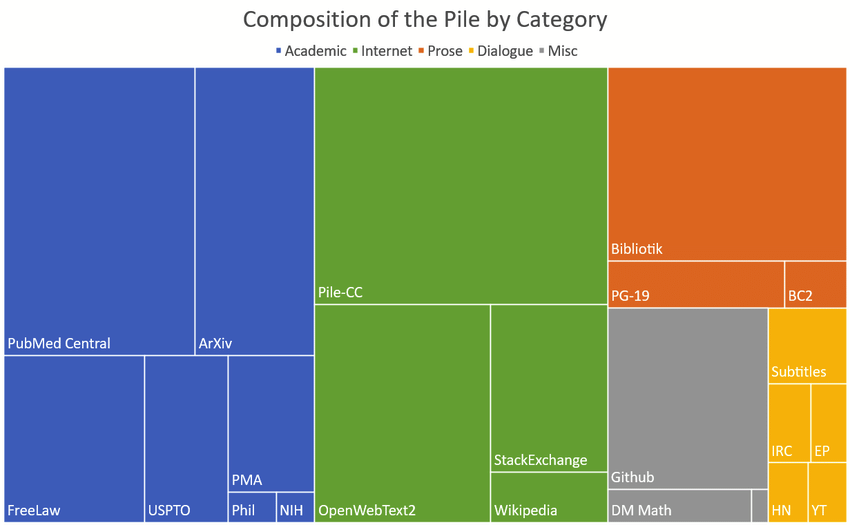
\includegraphics[width=\textwidth]{figures/Treemap-of-Pile-components-by-effective-size.png}
    \caption{Treemap of Pile components by effective size. SOURCE FROM THEPILE paper}
    \label{fig:flowchart}
\end{figure}


\subsection{Verified Smart Contracts}
\label{sec:verified-smart-contracts}
\url{https://github.com/andstor/verified-smart-contracts}
\url{https://huggingface.co/datasets/andstor/smart_contracts}

The Verified Smart Contracts dataset is a dataset consisting of verified Smart Contracts from Etherscan.io. This is real smmart contracts that are deployed to the Ethereum blockchain. A set of 100,000 to 200,000 contracts are provided, containing both Solidity and Vyper code.

\cref{tab:verified-smart-contracts-metrics} shows the metrics of the various (sub)datasets.

\begin{table}
    %\newcolumntype{Y}{>{\centering\arraybackslash}X}
    \def\arraystretch{1.5}
    \small
    \centering
    \caption{Verified Smart Contracts Metrics}
    \label{tab:verified-smart-contracts-metrics}
    \begin{tabularx}{\textwidth}{XXXX}
        \toprule
        \textbf{Component} & \textbf{Size} &  \textbf{Num rows} & \textbf{LoC*}\\
        \midrule
        Raw & 0.80 GiB & 2,217,692 & 839,665,295\\
        Flattened & 1.16 GiB & 136,969 & 97,529,473\\
        Inflated & 0.76 GiB & 186,397 & 53,843,305\\
        Parsed & 4.44 GiB & 4,434,014 & 29,965,185\\
        \bottomrule
    \end{tabularx}
\end{table}

LoC refers to the lines of source\_code. The Parsed dataset counts lines of func\_code + func\_documentation.

\subsubsection{Raw}
\label{sec:verified-smart-contracts-raw}
The raw dataset contains mostly the raw data from Etherscan, downloaded with the smart-contract-downlader tool, as described in \cref{sec:smart-contract-downloader}. All different contract formats (JSON, multi-file, etc.) are normalized to a flattened source code structure. 

\todo{Add stats on the raw dataset}

\subsubsection{Flattened}
\label{sec:verified-smart-contracts-flattened}

The flattened dataset is a filtered version  of the Raw dataset\cref{sec:verified-smart-contracts-raw}. It contains smart contracts, where every contract contains all required library code. Each "file" is marked in the source code with a comment stating the original file path: //File: path/to/file.sol. These are then filtered for uniqueness with a similarity threshold of 0.9. This means that all contracts whose code shares more than 90\% of the tokens will be discarded. The low uniqueness requirement is due to the often large amount of embedded library code. If the requirement is set to high, the actual contract code will be negligible compared to the library code. Most contracts will be discarded, and the resulting dataset would contain mostly unique library code. However, the dataset as a whole will have a large amount of duplicated libray code. From the 2,217,692 contracts, 2,080,723 duplications are found, giving a duplication percentage of 93.82\%. The resulting dataset consists of 136,969 contracts.

%Processing: 100%|██████| 74/74 [20:22<00:00, 16.51s/it, dupes=2081081/2217692 (93.84%)]

The following command prooduces the flattened dataset:

\lstinline[language=Python]!python script/filter_data.py -s parquet -o data/flattened --threshold 0.9!


\begin{lstlisting}[
    caption={Solidity standard JSON Input format.},
    label=lst:flattened-dataset-cmd,
    language=JSON]
{
  'contract_name': 'MiaKhalifaDAO',
  'contract_address': '0xb3862ca215d5ed2de22734ed001d701adf0a30b4',
  'language': 'Solidity',
  'source_code': '// File: @openzeppelin/contracts/utils/Strings.sol\r\n\r\n\r\n// OpenZeppelin Contracts v4.4.1 (utils/Strings.sol)\r\n\r\npragma solidity ^0.8.0;\r\n\r\n/**\r\n * @dev String operations.\r\n */\r\nlibrary Strings {\r\n...',
  'abi': '[{"inputs":[{"internalType":"uint256","name":"maxBatchSize_","type":"uint256"}...]',
  'compiler_version': 'v0.8.7+commit.e28d00a7',
  'optimization_used': False,
  'runs': 200,
  'constructor_arguments': '000000000000000000000000000000000000000000000000000000000000000a000...',
  'evm_version': 'Default',
  'library': '',
  'license_type': 'MIT',
  'proxy': False,
  'implementation': '',
  'swarm_source': 'ipfs://e490df69bd9ca50e1831a1ac82177e826fee459b0b085a00bd7a727c80d74089'
}
\end{lstlisting}



\subsubsection{Inflated}
\label{sec:verified-smart-contracts-inflated}
The inflated dataset is also based on the raw dataset. Each contract file in the dataset is split into its original representative files. This mitigates a lot of the problems of the flattened dataset in terms of duplicated library code. The library code would, along with other imported contract files, be split into separate contract records. The 2,217,692 "raw" smart contracts are inflated to a total of 5,403,136 separate contract files. These are then grouped by "file\_name" and filtered for uniqueness with a similarity threshold of 0.9. This should produce a dataset with a large amount of unique source code, with low quantities of library code. A total of 5,216,739 duplications are found, giving a duplication percentage of 96.56\%. The resulting dataset consists of 186,397 contracts.

%Processing: 100%|██████| 74/74 [22:50<00:00, 18.52s/it, dupes=5217191/5403136 (96.56%)]


\lstinline[language=Python]!python script/filter_data.py -s parquet -o data/inflated --split-files --threshold 0.9!
dupes=5217191/5403136 (96.56%)


\begin{lstlisting}[
    caption={Solidity standard JSON Input format.},
    label=lst:flattened-dataset-cmd,
    language=JSON]
    {
        'contract_name': 'PinkLemonade',
        'file_path': 'PinkLemonade.sol',
        'contract_address': '0x9a5be3cc368f01a0566a613aad7183783cff7eec',
        'language': 'Solidity',
        'source_code': '/**\r\n\r\nt.me/pinklemonadecoin\r\n*/\r\n\r\n// SPDX-License-Identifier: MIT\r\npragma solidity ^0.8.0;\r\n\r\n\r\n/*\r\n * @dev Provides information about the current execution context, including the\r\n * sender of the transaction and its data. While these are generally available...',
        'abi': '[{"inputs":[],"stateMutability":"nonpayable","type":"constructor"}...]',
        'compiler_version': 'v0.8.4+commit.c7e474f2',
        'optimization_used': False,
        'runs': 200,
        'constructor_arguments': '',
        'evm_version': 'Default',
        'library': '',
        'license_type': 'MIT',
        'proxy': False,
        'implementation': '',
        'swarm_source': 'ipfs://eb0ac9491a04e7a196280fd27ce355a85d79b34c7b0a83ab606d27972a06050c'
      }
      
      
\end{lstlisting}

\begin{figure}[ht]
    \centering
    %% Creator: Matplotlib, PGF backend
%%
%% To include the figure in your LaTeX document, write
%%   \input{<filename>.pgf}
%%
%% Make sure the required packages are loaded in your preamble
%%   \usepackage{pgf}
%%
%% and, on pdftex
%%   \usepackage[utf8]{inputenc}\DeclareUnicodeCharacter{2212}{-}
%%
%% or, on luatex and xetex
%%   \usepackage{unicode-math}
%%
%% Figures using additional raster images can only be included by \input if
%% they are in the same directory as the main LaTeX file. For loading figures
%% from other directories you can use the `import` package
%%   \usepackage{import}
%%
%% and then include the figures with
%%   \import{<path to file>}{<filename>.pgf}
%%
%% Matplotlib used the following preamble
%%
\begingroup%
\makeatletter%
\begin{pgfpicture}%
\pgfpathrectangle{\pgfpointorigin}{\pgfqpoint{3.449272in}{3.773420in}}%
\pgfusepath{use as bounding box, clip}%
\begin{pgfscope}%
\pgfsetbuttcap%
\pgfsetmiterjoin%
\definecolor{currentfill}{rgb}{1.000000,1.000000,1.000000}%
\pgfsetfillcolor{currentfill}%
\pgfsetlinewidth{0.000000pt}%
\definecolor{currentstroke}{rgb}{1.000000,1.000000,1.000000}%
\pgfsetstrokecolor{currentstroke}%
\pgfsetdash{}{0pt}%
\pgfpathmoveto{\pgfqpoint{0.000000in}{-0.000000in}}%
\pgfpathlineto{\pgfqpoint{3.449272in}{-0.000000in}}%
\pgfpathlineto{\pgfqpoint{3.449272in}{3.773420in}}%
\pgfpathlineto{\pgfqpoint{0.000000in}{3.773420in}}%
\pgfpathclose%
\pgfusepath{fill}%
\end{pgfscope}%
\begin{pgfscope}%
\pgfsetbuttcap%
\pgfsetmiterjoin%
\definecolor{currentfill}{rgb}{0.475341,0.000000,0.943137}%
\pgfsetfillcolor{currentfill}%
\pgfsetfillopacity{0.700000}%
\pgfsetlinewidth{0.000000pt}%
\definecolor{currentstroke}{rgb}{0.000000,0.000000,0.000000}%
\pgfsetstrokecolor{currentstroke}%
\pgfsetstrokeopacity{0.700000}%
\pgfsetdash{}{0pt}%
\pgfpathmoveto{\pgfqpoint{2.651052in}{2.128968in}}%
\pgfpathcurveto{\pgfqpoint{2.651052in}{2.133588in}}{\pgfqpoint{2.651020in}{2.138209in}}{\pgfqpoint{2.650958in}{2.142829in}}%
\pgfpathcurveto{\pgfqpoint{2.650895in}{2.147449in}}{\pgfqpoint{2.650801in}{2.152068in}}{\pgfqpoint{2.650675in}{2.156687in}}%
\pgfpathlineto{\pgfqpoint{2.140693in}{2.142827in}}%
\pgfpathcurveto{\pgfqpoint{2.140756in}{2.140518in}}{\pgfqpoint{2.140803in}{2.138208in}}{\pgfqpoint{2.140834in}{2.135898in}}%
\pgfpathcurveto{\pgfqpoint{2.140866in}{2.133588in}}{\pgfqpoint{2.140881in}{2.131278in}}{\pgfqpoint{2.140881in}{2.128968in}}%
\pgfpathlineto{\pgfqpoint{2.651052in}{2.128968in}}%
\pgfpathclose%
\pgfusepath{fill}%
\end{pgfscope}%
\begin{pgfscope}%
\pgfsetbuttcap%
\pgfsetmiterjoin%
\definecolor{currentfill}{rgb}{0.882745,0.000000,0.111414}%
\pgfsetfillcolor{currentfill}%
\pgfsetfillopacity{0.700000}%
\pgfsetlinewidth{0.000000pt}%
\definecolor{currentstroke}{rgb}{0.000000,0.000000,0.000000}%
\pgfsetstrokecolor{currentstroke}%
\pgfsetstrokeopacity{0.700000}%
\pgfsetdash{}{0pt}%
\pgfpathmoveto{\pgfqpoint{2.650675in}{2.156687in}}%
\pgfpathcurveto{\pgfqpoint{2.643613in}{2.416544in}}{\pgfqpoint{2.537505in}{2.664127in}}{\pgfqpoint{2.354202in}{2.848452in}}%
\pgfpathcurveto{\pgfqpoint{2.170898in}{3.032777in}}{\pgfqpoint{1.923908in}{3.140258in}}{\pgfqpoint{1.664093in}{3.148763in}}%
\pgfpathcurveto{\pgfqpoint{1.404279in}{3.157268in}}{\pgfqpoint{1.150788in}{3.066169in}}{\pgfqpoint{0.955822in}{2.894227in}}%
\pgfpathcurveto{\pgfqpoint{0.760856in}{2.722285in}}{\pgfqpoint{0.638784in}{2.482171in}}{\pgfqpoint{0.614743in}{2.223332in}}%
\pgfpathlineto{\pgfqpoint{1.122727in}{2.176150in}}%
\pgfpathcurveto{\pgfqpoint{1.134747in}{2.305570in}}{\pgfqpoint{1.195784in}{2.425626in}}{\pgfqpoint{1.293267in}{2.511598in}}%
\pgfpathcurveto{\pgfqpoint{1.390750in}{2.597569in}}{\pgfqpoint{1.517495in}{2.643118in}}{\pgfqpoint{1.647402in}{2.638866in}}%
\pgfpathcurveto{\pgfqpoint{1.777309in}{2.634613in}}{\pgfqpoint{1.900804in}{2.580872in}}{\pgfqpoint{1.992456in}{2.488710in}}%
\pgfpathcurveto{\pgfqpoint{2.084108in}{2.396548in}}{\pgfqpoint{2.137162in}{2.272756in}}{\pgfqpoint{2.140693in}{2.142827in}}%
\pgfpathlineto{\pgfqpoint{2.650675in}{2.156687in}}%
\pgfpathclose%
\pgfusepath{fill}%
\end{pgfscope}%
\begin{pgfscope}%
\pgfsetbuttcap%
\pgfsetmiterjoin%
\definecolor{currentfill}{rgb}{0.000000,0.786667,0.312353}%
\pgfsetfillcolor{currentfill}%
\pgfsetfillopacity{0.700000}%
\pgfsetlinewidth{0.000000pt}%
\definecolor{currentstroke}{rgb}{0.000000,0.000000,0.000000}%
\pgfsetstrokecolor{currentstroke}%
\pgfsetstrokeopacity{0.700000}%
\pgfsetdash{}{0pt}%
\pgfpathmoveto{\pgfqpoint{0.614743in}{2.223332in}}%
\pgfpathcurveto{\pgfqpoint{0.611982in}{2.193606in}}{\pgfqpoint{0.610527in}{2.163774in}}{\pgfqpoint{0.610382in}{2.133921in}}%
\pgfpathcurveto{\pgfqpoint{0.610237in}{2.104068in}}{\pgfqpoint{0.611402in}{2.074223in}}{\pgfqpoint{0.613874in}{2.044472in}}%
\pgfpathlineto{\pgfqpoint{1.122293in}{2.086720in}}%
\pgfpathcurveto{\pgfqpoint{1.121057in}{2.101596in}}{\pgfqpoint{1.120474in}{2.116518in}}{\pgfqpoint{1.120546in}{2.131445in}}%
\pgfpathcurveto{\pgfqpoint{1.120619in}{2.146371in}}{\pgfqpoint{1.121346in}{2.161287in}}{\pgfqpoint{1.122727in}{2.176150in}}%
\pgfpathlineto{\pgfqpoint{0.614743in}{2.223332in}}%
\pgfpathclose%
\pgfusepath{fill}%
\end{pgfscope}%
\begin{pgfscope}%
\pgfsetbuttcap%
\pgfsetmiterjoin%
\definecolor{currentfill}{rgb}{0.930307,0.285685,0.029301}%
\pgfsetfillcolor{currentfill}%
\pgfsetfillopacity{0.700000}%
\pgfsetlinewidth{0.000000pt}%
\definecolor{currentstroke}{rgb}{0.000000,0.000000,0.000000}%
\pgfsetstrokecolor{currentstroke}%
\pgfsetstrokeopacity{0.700000}%
\pgfsetdash{}{0pt}%
\pgfpathmoveto{\pgfqpoint{0.613874in}{2.044472in}}%
\pgfpathcurveto{\pgfqpoint{0.633145in}{1.812567in}}{\pgfqpoint{0.731182in}{1.594089in}}{\pgfqpoint{0.891613in}{1.425527in}}%
\pgfpathcurveto{\pgfqpoint{1.052044in}{1.256964in}}{\pgfqpoint{1.265411in}{1.148252in}}{\pgfqpoint{1.496081in}{1.117548in}}%
\pgfpathlineto{\pgfqpoint{1.563396in}{1.623258in}}%
\pgfpathcurveto{\pgfqpoint{1.448061in}{1.638610in}}{\pgfqpoint{1.341377in}{1.692966in}}{\pgfqpoint{1.261162in}{1.777247in}}%
\pgfpathcurveto{\pgfqpoint{1.180946in}{1.861529in}}{\pgfqpoint{1.131928in}{1.970768in}}{\pgfqpoint{1.122293in}{2.086720in}}%
\pgfpathlineto{\pgfqpoint{0.613874in}{2.044472in}}%
\pgfpathclose%
\pgfusepath{fill}%
\end{pgfscope}%
\begin{pgfscope}%
\pgfsetbuttcap%
\pgfsetmiterjoin%
\definecolor{currentfill}{rgb}{0.063700,0.382199,0.851986}%
\pgfsetfillcolor{currentfill}%
\pgfsetfillopacity{0.700000}%
\pgfsetlinewidth{0.000000pt}%
\definecolor{currentstroke}{rgb}{0.000000,0.000000,0.000000}%
\pgfsetstrokecolor{currentstroke}%
\pgfsetstrokeopacity{0.700000}%
\pgfsetdash{}{0pt}%
\pgfpathmoveto{\pgfqpoint{1.496081in}{1.117548in}}%
\pgfpathcurveto{\pgfqpoint{1.640169in}{1.098369in}}{\pgfqpoint{1.786706in}{1.110199in}}{\pgfqpoint{1.925851in}{1.152245in}}%
\pgfpathcurveto{\pgfqpoint{2.064996in}{1.194291in}}{\pgfqpoint{2.193564in}{1.265590in}}{\pgfqpoint{2.302919in}{1.361354in}}%
\pgfpathcurveto{\pgfqpoint{2.412274in}{1.457117in}}{\pgfqpoint{2.499914in}{1.575153in}}{\pgfqpoint{2.559952in}{1.707534in}}%
\pgfpathcurveto{\pgfqpoint{2.619990in}{1.839914in}}{\pgfqpoint{2.651052in}{1.983609in}}{\pgfqpoint{2.651052in}{2.128968in}}%
\pgfpathlineto{\pgfqpoint{2.140881in}{2.128968in}}%
\pgfpathcurveto{\pgfqpoint{2.140881in}{2.056289in}}{\pgfqpoint{2.125350in}{1.984441in}}{\pgfqpoint{2.095331in}{1.918251in}}%
\pgfpathcurveto{\pgfqpoint{2.065312in}{1.852060in}}{\pgfqpoint{2.021493in}{1.793043in}}{\pgfqpoint{1.966815in}{1.745161in}}%
\pgfpathcurveto{\pgfqpoint{1.912137in}{1.697279in}}{\pgfqpoint{1.847854in}{1.661630in}}{\pgfqpoint{1.778281in}{1.640607in}}%
\pgfpathcurveto{\pgfqpoint{1.708709in}{1.619584in}}{\pgfqpoint{1.635440in}{1.613668in}}{\pgfqpoint{1.563396in}{1.623258in}}%
\pgfpathlineto{\pgfqpoint{1.496081in}{1.117548in}}%
\pgfpathclose%
\pgfusepath{fill}%
\end{pgfscope}%
\begin{pgfscope}%
\pgfsetbuttcap%
\pgfsetmiterjoin%
\definecolor{currentfill}{rgb}{0.475341,0.000000,0.943137}%
\pgfsetfillcolor{currentfill}%
\pgfsetfillopacity{0.700000}%
\pgfsetlinewidth{0.000000pt}%
\definecolor{currentstroke}{rgb}{0.000000,0.000000,0.000000}%
\pgfsetstrokecolor{currentstroke}%
\pgfsetstrokeopacity{0.700000}%
\pgfsetdash{}{0pt}%
\pgfpathmoveto{\pgfqpoint{3.161222in}{2.128968in}}%
\pgfpathcurveto{\pgfqpoint{3.161222in}{2.135899in}}{\pgfqpoint{3.161175in}{2.142829in}}{\pgfqpoint{3.161081in}{2.149759in}}%
\pgfpathcurveto{\pgfqpoint{3.160987in}{2.156689in}}{\pgfqpoint{3.160846in}{2.163618in}}{\pgfqpoint{3.160658in}{2.170546in}}%
\pgfpathlineto{\pgfqpoint{2.650675in}{2.156687in}}%
\pgfpathcurveto{\pgfqpoint{2.650801in}{2.152068in}}{\pgfqpoint{2.650895in}{2.147449in}}{\pgfqpoint{2.650958in}{2.142829in}}%
\pgfpathcurveto{\pgfqpoint{2.651020in}{2.138209in}}{\pgfqpoint{2.651052in}{2.133588in}}{\pgfqpoint{2.651052in}{2.128968in}}%
\pgfpathlineto{\pgfqpoint{3.161222in}{2.128968in}}%
\pgfpathclose%
\pgfusepath{fill}%
\end{pgfscope}%
\begin{pgfscope}%
\pgfsetbuttcap%
\pgfsetmiterjoin%
\definecolor{currentfill}{rgb}{0.882745,0.000000,0.111414}%
\pgfsetfillcolor{currentfill}%
\pgfsetfillopacity{0.700000}%
\pgfsetlinewidth{0.000000pt}%
\definecolor{currentstroke}{rgb}{0.000000,0.000000,0.000000}%
\pgfsetstrokecolor{currentstroke}%
\pgfsetstrokeopacity{0.700000}%
\pgfsetdash{}{0pt}%
\pgfpathmoveto{\pgfqpoint{3.160658in}{2.170546in}}%
\pgfpathcurveto{\pgfqpoint{3.159046in}{2.229862in}}{\pgfqpoint{3.153985in}{2.289035in}}{\pgfqpoint{3.145503in}{2.347763in}}%
\pgfpathcurveto{\pgfqpoint{3.137020in}{2.406492in}}{\pgfqpoint{3.125129in}{2.464678in}}{\pgfqpoint{3.109890in}{2.522026in}}%
\pgfpathlineto{\pgfqpoint{2.616830in}{2.391007in}}%
\pgfpathcurveto{\pgfqpoint{2.626990in}{2.352775in}}{\pgfqpoint{2.634917in}{2.313984in}}{\pgfqpoint{2.640572in}{2.274832in}}%
\pgfpathcurveto{\pgfqpoint{2.646227in}{2.235679in}}{\pgfqpoint{2.649601in}{2.196231in}}{\pgfqpoint{2.650675in}{2.156687in}}%
\pgfpathlineto{\pgfqpoint{3.160658in}{2.170546in}}%
\pgfpathclose%
\pgfusepath{fill}%
\end{pgfscope}%
\begin{pgfscope}%
\pgfsetbuttcap%
\pgfsetmiterjoin%
\definecolor{currentfill}{rgb}{0.917292,0.307374,0.323876}%
\pgfsetfillcolor{currentfill}%
\pgfsetfillopacity{0.700000}%
\pgfsetlinewidth{0.000000pt}%
\definecolor{currentstroke}{rgb}{0.000000,0.000000,0.000000}%
\pgfsetstrokecolor{currentstroke}%
\pgfsetstrokeopacity{0.700000}%
\pgfsetdash{}{0pt}%
\pgfpathmoveto{\pgfqpoint{3.109890in}{2.522026in}}%
\pgfpathcurveto{\pgfqpoint{3.091225in}{2.592268in}}{\pgfqpoint{3.067580in}{2.661092in}}{\pgfqpoint{3.039134in}{2.727974in}}%
\pgfpathcurveto{\pgfqpoint{3.010689in}{2.794857in}}{\pgfqpoint{2.977516in}{2.859628in}}{\pgfqpoint{2.939867in}{2.921797in}}%
\pgfpathlineto{\pgfqpoint{2.503481in}{2.657520in}}%
\pgfpathcurveto{\pgfqpoint{2.528581in}{2.616075in}}{\pgfqpoint{2.550696in}{2.572894in}}{\pgfqpoint{2.569660in}{2.528306in}}%
\pgfpathcurveto{\pgfqpoint{2.588623in}{2.483717in}}{\pgfqpoint{2.604387in}{2.437835in}}{\pgfqpoint{2.616830in}{2.391007in}}%
\pgfpathlineto{\pgfqpoint{3.109890in}{2.522026in}}%
\pgfpathclose%
\pgfusepath{fill}%
\end{pgfscope}%
\begin{pgfscope}%
\pgfsetbuttcap%
\pgfsetmiterjoin%
\definecolor{currentfill}{rgb}{0.989063,0.592703,0.504860}%
\pgfsetfillcolor{currentfill}%
\pgfsetfillopacity{0.700000}%
\pgfsetlinewidth{0.000000pt}%
\definecolor{currentstroke}{rgb}{0.000000,0.000000,0.000000}%
\pgfsetstrokecolor{currentstroke}%
\pgfsetstrokeopacity{0.700000}%
\pgfsetdash{}{0pt}%
\pgfpathmoveto{\pgfqpoint{2.939867in}{2.921797in}}%
\pgfpathcurveto{\pgfqpoint{2.822564in}{3.115492in}}{\pgfqpoint{2.663723in}{3.280762in}}{\pgfqpoint{2.474832in}{3.405653in}}%
\pgfpathcurveto{\pgfqpoint{2.285940in}{3.530545in}}{\pgfqpoint{2.071665in}{3.611973in}}{\pgfqpoint{1.847502in}{3.644048in}}%
\pgfpathlineto{\pgfqpoint{1.775238in}{3.139021in}}%
\pgfpathcurveto{\pgfqpoint{1.924680in}{3.117638in}}{\pgfqpoint{2.067531in}{3.063353in}}{\pgfqpoint{2.193458in}{2.980092in}}%
\pgfpathcurveto{\pgfqpoint{2.319386in}{2.896831in}}{\pgfqpoint{2.425280in}{2.786651in}}{\pgfqpoint{2.503481in}{2.657520in}}%
\pgfpathlineto{\pgfqpoint{2.939867in}{2.921797in}}%
\pgfpathclose%
\pgfusepath{fill}%
\end{pgfscope}%
\begin{pgfscope}%
\pgfsetbuttcap%
\pgfsetmiterjoin%
\definecolor{currentfill}{rgb}{0.991894,0.815723,0.745126}%
\pgfsetfillcolor{currentfill}%
\pgfsetfillopacity{0.700000}%
\pgfsetlinewidth{0.000000pt}%
\definecolor{currentstroke}{rgb}{0.000000,0.000000,0.000000}%
\pgfsetstrokecolor{currentstroke}%
\pgfsetstrokeopacity{0.700000}%
\pgfsetdash{}{0pt}%
\pgfpathmoveto{\pgfqpoint{1.847502in}{3.644048in}}%
\pgfpathcurveto{\pgfqpoint{1.642231in}{3.673420in}}{\pgfqpoint{1.433115in}{3.660771in}}{\pgfqpoint{1.232881in}{3.606871in}}%
\pgfpathcurveto{\pgfqpoint{1.032647in}{3.552971in}}{\pgfqpoint{0.845439in}{3.458936in}}{\pgfqpoint{0.682651in}{3.330487in}}%
\pgfpathcurveto{\pgfqpoint{0.519863in}{3.202039in}}{\pgfqpoint{0.384864in}{3.041837in}}{\pgfqpoint{0.285870in}{2.859631in}}%
\pgfpathcurveto{\pgfqpoint{0.186876in}{2.677425in}}{\pgfqpoint{0.125936in}{2.476986in}}{\pgfqpoint{0.106759in}{2.270513in}}%
\pgfpathlineto{\pgfqpoint{0.614743in}{2.223332in}}%
\pgfpathcurveto{\pgfqpoint{0.627528in}{2.360980in}}{\pgfqpoint{0.668154in}{2.494606in}}{\pgfqpoint{0.734150in}{2.616077in}}%
\pgfpathcurveto{\pgfqpoint{0.800146in}{2.737548in}}{\pgfqpoint{0.890146in}{2.844349in}}{\pgfqpoint{0.998671in}{2.929981in}}%
\pgfpathcurveto{\pgfqpoint{1.107197in}{3.015613in}}{\pgfqpoint{1.232001in}{3.078303in}}{\pgfqpoint{1.365491in}{3.114237in}}%
\pgfpathcurveto{\pgfqpoint{1.498980in}{3.150170in}}{\pgfqpoint{1.638391in}{3.158603in}}{\pgfqpoint{1.775238in}{3.139021in}}%
\pgfpathlineto{\pgfqpoint{1.847502in}{3.644048in}}%
\pgfpathclose%
\pgfusepath{fill}%
\end{pgfscope}%
\begin{pgfscope}%
\pgfsetbuttcap%
\pgfsetmiterjoin%
\definecolor{currentfill}{rgb}{0.000000,0.786667,0.312353}%
\pgfsetfillcolor{currentfill}%
\pgfsetfillopacity{0.700000}%
\pgfsetlinewidth{0.000000pt}%
\definecolor{currentstroke}{rgb}{0.000000,0.000000,0.000000}%
\pgfsetstrokecolor{currentstroke}%
\pgfsetstrokeopacity{0.700000}%
\pgfsetdash{}{0pt}%
\pgfpathmoveto{\pgfqpoint{0.106759in}{2.270513in}}%
\pgfpathcurveto{\pgfqpoint{0.102617in}{2.225925in}}{\pgfqpoint{0.100435in}{2.181177in}}{\pgfqpoint{0.100217in}{2.136397in}}%
\pgfpathcurveto{\pgfqpoint{0.100000in}{2.091618in}}{\pgfqpoint{0.101748in}{2.046851in}}{\pgfqpoint{0.105456in}{2.002225in}}%
\pgfpathlineto{\pgfqpoint{0.613874in}{2.044472in}}%
\pgfpathcurveto{\pgfqpoint{0.611402in}{2.074223in}}{\pgfqpoint{0.610237in}{2.104068in}}{\pgfqpoint{0.610382in}{2.133921in}}%
\pgfpathcurveto{\pgfqpoint{0.610527in}{2.163774in}}{\pgfqpoint{0.611982in}{2.193606in}}{\pgfqpoint{0.614743in}{2.223332in}}%
\pgfpathlineto{\pgfqpoint{0.106759in}{2.270513in}}%
\pgfpathclose%
\pgfusepath{fill}%
\end{pgfscope}%
\begin{pgfscope}%
\pgfsetbuttcap%
\pgfsetmiterjoin%
\definecolor{currentfill}{rgb}{0.930307,0.285685,0.029301}%
\pgfsetfillcolor{currentfill}%
\pgfsetfillopacity{0.700000}%
\pgfsetlinewidth{0.000000pt}%
\definecolor{currentstroke}{rgb}{0.000000,0.000000,0.000000}%
\pgfsetstrokecolor{currentstroke}%
\pgfsetstrokeopacity{0.700000}%
\pgfsetdash{}{0pt}%
\pgfpathmoveto{\pgfqpoint{0.105456in}{2.002225in}}%
\pgfpathcurveto{\pgfqpoint{0.124422in}{1.773989in}}{\pgfqpoint{0.194377in}{1.552894in}}{\pgfqpoint{0.310149in}{1.355287in}}%
\pgfpathcurveto{\pgfqpoint{0.425921in}{1.157681in}}{\pgfqpoint{0.584584in}{0.988558in}}{\pgfqpoint{0.774407in}{0.860422in}}%
\pgfpathlineto{\pgfqpoint{1.059841in}{1.283271in}}%
\pgfpathcurveto{\pgfqpoint{0.933293in}{1.368695in}}{\pgfqpoint{0.827518in}{1.481444in}}{\pgfqpoint{0.750336in}{1.613181in}}%
\pgfpathcurveto{\pgfqpoint{0.673155in}{1.744918in}}{\pgfqpoint{0.626518in}{1.892315in}}{\pgfqpoint{0.613874in}{2.044472in}}%
\pgfpathlineto{\pgfqpoint{0.105456in}{2.002225in}}%
\pgfpathclose%
\pgfusepath{fill}%
\end{pgfscope}%
\begin{pgfscope}%
\pgfsetbuttcap%
\pgfsetmiterjoin%
\definecolor{currentfill}{rgb}{0.995815,0.464325,0.203521}%
\pgfsetfillcolor{currentfill}%
\pgfsetfillopacity{0.700000}%
\pgfsetlinewidth{0.000000pt}%
\definecolor{currentstroke}{rgb}{0.000000,0.000000,0.000000}%
\pgfsetstrokecolor{currentstroke}%
\pgfsetstrokeopacity{0.700000}%
\pgfsetdash{}{0pt}%
\pgfpathmoveto{\pgfqpoint{0.774407in}{0.860422in}}%
\pgfpathcurveto{\pgfqpoint{0.872074in}{0.794494in}}{\pgfqpoint{0.977029in}{0.740065in}}{\pgfqpoint{1.087184in}{0.698219in}}%
\pgfpathcurveto{\pgfqpoint{1.197340in}{0.656372in}}{\pgfqpoint{1.311960in}{0.627386in}}{\pgfqpoint{1.428766in}{0.611838in}}%
\pgfpathlineto{\pgfqpoint{1.496081in}{1.117548in}}%
\pgfpathcurveto{\pgfqpoint{1.418210in}{1.127913in}}{\pgfqpoint{1.341797in}{1.147237in}}{\pgfqpoint{1.268360in}{1.175135in}}%
\pgfpathcurveto{\pgfqpoint{1.194923in}{1.203033in}}{\pgfqpoint{1.124953in}{1.239319in}}{\pgfqpoint{1.059841in}{1.283271in}}%
\pgfpathlineto{\pgfqpoint{0.774407in}{0.860422in}}%
\pgfpathclose%
\pgfusepath{fill}%
\end{pgfscope}%
\begin{pgfscope}%
\pgfsetbuttcap%
\pgfsetmiterjoin%
\definecolor{currentfill}{rgb}{0.063700,0.382199,0.851986}%
\pgfsetfillcolor{currentfill}%
\pgfsetfillopacity{0.700000}%
\pgfsetlinewidth{0.000000pt}%
\definecolor{currentstroke}{rgb}{0.000000,0.000000,0.000000}%
\pgfsetstrokecolor{currentstroke}%
\pgfsetstrokeopacity{0.700000}%
\pgfsetdash{}{0pt}%
\pgfpathmoveto{\pgfqpoint{1.428766in}{0.611838in}}%
\pgfpathcurveto{\pgfqpoint{1.644898in}{0.583069in}}{\pgfqpoint{1.864704in}{0.600815in}}{\pgfqpoint{2.073422in}{0.663884in}}%
\pgfpathcurveto{\pgfqpoint{2.282139in}{0.726953in}}{\pgfqpoint{2.474990in}{0.833901in}}{\pgfqpoint{2.639023in}{0.977546in}}%
\pgfpathcurveto{\pgfqpoint{2.803056in}{1.121192in}}{\pgfqpoint{2.934515in}{1.298245in}}{\pgfqpoint{3.024572in}{1.496816in}}%
\pgfpathcurveto{\pgfqpoint{3.114629in}{1.695387in}}{\pgfqpoint{3.161222in}{1.910930in}}{\pgfqpoint{3.161222in}{2.128968in}}%
\pgfpathlineto{\pgfqpoint{2.651052in}{2.128968in}}%
\pgfpathcurveto{\pgfqpoint{2.651052in}{1.983609in}}{\pgfqpoint{2.619990in}{1.839914in}}{\pgfqpoint{2.559952in}{1.707534in}}%
\pgfpathcurveto{\pgfqpoint{2.499914in}{1.575153in}}{\pgfqpoint{2.412274in}{1.457117in}}{\pgfqpoint{2.302919in}{1.361354in}}%
\pgfpathcurveto{\pgfqpoint{2.193564in}{1.265590in}}{\pgfqpoint{2.064996in}{1.194291in}}{\pgfqpoint{1.925851in}{1.152245in}}%
\pgfpathcurveto{\pgfqpoint{1.786706in}{1.110199in}}{\pgfqpoint{1.640169in}{1.098369in}}{\pgfqpoint{1.496081in}{1.117548in}}%
\pgfpathlineto{\pgfqpoint{1.428766in}{0.611838in}}%
\pgfpathclose%
\pgfusepath{fill}%
\end{pgfscope}%
\begin{pgfscope}%
\definecolor{textcolor}{rgb}{0.000000,0.000000,0.000000}%
\pgfsetstrokecolor{textcolor}%
\pgfsetfillcolor{textcolor}%
\pgftext[x=2.344884in,y=2.138671in,left,]{\color{textcolor}\rmfamily\fontsize{10.000000}{12.000000}\selectfont E}%
\end{pgfscope}%
\begin{pgfscope}%
\definecolor{textcolor}{rgb}{0.000000,0.000000,0.000000}%
\pgfsetstrokecolor{textcolor}%
\pgfsetfillcolor{textcolor}%
\pgftext[x=1.654078in,y=2.842825in,left,]{\color{textcolor}\rmfamily\fontsize{10.000000}{12.000000}\selectfont H}%
\end{pgfscope}%
\begin{pgfscope}%
\definecolor{textcolor}{rgb}{0.000000,0.000000,0.000000}%
\pgfsetstrokecolor{textcolor}%
\pgfsetfillcolor{textcolor}%
\pgftext[x=0.916481in,y=2.132435in,right,]{\color{textcolor}\rmfamily\fontsize{10.000000}{12.000000}\selectfont L}%
\end{pgfscope}%
\begin{pgfscope}%
\definecolor{textcolor}{rgb}{0.000000,0.000000,0.000000}%
\pgfsetstrokecolor{textcolor}%
\pgfsetfillcolor{textcolor}%
\pgftext[x=1.113342in,y=1.636559in,right,]{\color{textcolor}\rmfamily\fontsize{10.000000}{12.000000}\selectfont M}%
\end{pgfscope}%
\begin{pgfscope}%
\definecolor{textcolor}{rgb}{0.000000,0.000000,0.000000}%
\pgfsetstrokecolor{textcolor}%
\pgfsetfillcolor{textcolor}%
\pgftext[x=2.101257in,y=1.591638in,left,]{\color{textcolor}\rmfamily\fontsize{10.000000}{12.000000}\selectfont S}%
\end{pgfscope}%
\begin{pgfscope}%
\definecolor{textcolor}{rgb}{0.000000,0.000000,0.000000}%
\pgfsetstrokecolor{textcolor}%
\pgfsetfillcolor{textcolor}%
\pgftext[x=2.838003in,y=2.145370in,left,]{\color{textcolor}\rmfamily\fontsize{10.000000}{12.000000}\selectfont E}%
\end{pgfscope}%
\begin{pgfscope}%
\definecolor{textcolor}{rgb}{0.000000,0.000000,0.000000}%
\pgfsetstrokecolor{textcolor}%
\pgfsetfillcolor{textcolor}%
\pgftext[x=2.825713in,y=2.301573in,left,]{\color{textcolor}\rmfamily\fontsize{10.000000}{12.000000}\selectfont H}%
\end{pgfscope}%
\begin{pgfscope}%
\definecolor{textcolor}{rgb}{0.000000,0.000000,0.000000}%
\pgfsetstrokecolor{textcolor}%
\pgfsetfillcolor{textcolor}%
\pgftext[x=2.741801in,y=2.601518in,left,]{\color{textcolor}\rmfamily\fontsize{10.000000}{12.000000}\selectfont HL}%
\end{pgfscope}%
\begin{pgfscope}%
\definecolor{textcolor}{rgb}{0.000000,0.000000,0.000000}%
\pgfsetstrokecolor{textcolor}%
\pgfsetfillcolor{textcolor}%
\pgftext[x=2.296628in,y=3.136131in,left,]{\color{textcolor}\rmfamily\fontsize{10.000000}{12.000000}\selectfont HM}%
\end{pgfscope}%
\begin{pgfscope}%
\definecolor{textcolor}{rgb}{0.000000,0.000000,0.000000}%
\pgfsetstrokecolor{textcolor}%
\pgfsetfillcolor{textcolor}%
\pgftext[x=0.882797in,y=3.076833in,right,]{\color{textcolor}\rmfamily\fontsize{10.000000}{12.000000}\selectfont HML}%
\end{pgfscope}%
\begin{pgfscope}%
\definecolor{textcolor}{rgb}{0.000000,0.000000,0.000000}%
\pgfsetstrokecolor{textcolor}%
\pgfsetfillcolor{textcolor}%
\pgftext[x=0.423322in,y=2.134829in,right,]{\color{textcolor}\rmfamily\fontsize{10.000000}{12.000000}\selectfont L}%
\end{pgfscope}%
\begin{pgfscope}%
\definecolor{textcolor}{rgb}{0.000000,0.000000,0.000000}%
\pgfsetstrokecolor{textcolor}%
\pgfsetfillcolor{textcolor}%
\pgftext[x=0.588934in,y=1.518620in,right,]{\color{textcolor}\rmfamily\fontsize{10.000000}{12.000000}\selectfont M}%
\end{pgfscope}%
\begin{pgfscope}%
\definecolor{textcolor}{rgb}{0.000000,0.000000,0.000000}%
\pgfsetstrokecolor{textcolor}%
\pgfsetfillcolor{textcolor}%
\pgftext[x=1.201929in,y=1.000266in,right,]{\color{textcolor}\rmfamily\fontsize{10.000000}{12.000000}\selectfont ML}%
\end{pgfscope}%
\begin{pgfscope}%
\definecolor{textcolor}{rgb}{0.000000,0.000000,0.000000}%
\pgfsetstrokecolor{textcolor}%
\pgfsetfillcolor{textcolor}%
\pgftext[x=2.426157in,y=1.220624in,left,]{\color{textcolor}\rmfamily\fontsize{10.000000}{12.000000}\selectfont S}%
\end{pgfscope}%
\begin{pgfscope}%
\pgfsetbuttcap%
\pgfsetmiterjoin%
\definecolor{currentfill}{rgb}{0.475341,0.000000,0.943137}%
\pgfsetfillcolor{currentfill}%
\pgfsetfillopacity{0.700000}%
\pgfsetlinewidth{1.003750pt}%
\definecolor{currentstroke}{rgb}{0.475341,0.000000,0.943137}%
\pgfsetstrokecolor{currentstroke}%
\pgfsetstrokeopacity{0.700000}%
\pgfsetdash{}{0pt}%
\pgfpathmoveto{\pgfqpoint{0.352742in}{0.376234in}}%
\pgfpathlineto{\pgfqpoint{0.630520in}{0.376234in}}%
\pgfpathlineto{\pgfqpoint{0.630520in}{0.473457in}}%
\pgfpathlineto{\pgfqpoint{0.352742in}{0.473457in}}%
\pgfpathclose%
\pgfusepath{stroke,fill}%
\end{pgfscope}%
\begin{pgfscope}%
\definecolor{textcolor}{rgb}{0.000000,0.000000,0.000000}%
\pgfsetstrokecolor{textcolor}%
\pgfsetfillcolor{textcolor}%
\pgftext[x=0.741631in,y=0.376234in,left,base]{\color{textcolor}\rmfamily\fontsize{10.000000}{12.000000}\selectfont Error}%
\end{pgfscope}%
\begin{pgfscope}%
\pgfsetbuttcap%
\pgfsetmiterjoin%
\definecolor{currentfill}{rgb}{0.882745,0.000000,0.111414}%
\pgfsetfillcolor{currentfill}%
\pgfsetfillopacity{0.700000}%
\pgfsetlinewidth{1.003750pt}%
\definecolor{currentstroke}{rgb}{0.882745,0.000000,0.111414}%
\pgfsetstrokecolor{currentstroke}%
\pgfsetstrokeopacity{0.700000}%
\pgfsetdash{}{0pt}%
\pgfpathmoveto{\pgfqpoint{0.352742in}{0.182562in}}%
\pgfpathlineto{\pgfqpoint{0.630520in}{0.182562in}}%
\pgfpathlineto{\pgfqpoint{0.630520in}{0.279784in}}%
\pgfpathlineto{\pgfqpoint{0.352742in}{0.279784in}}%
\pgfpathclose%
\pgfusepath{stroke,fill}%
\end{pgfscope}%
\begin{pgfscope}%
\definecolor{textcolor}{rgb}{0.000000,0.000000,0.000000}%
\pgfsetstrokecolor{textcolor}%
\pgfsetfillcolor{textcolor}%
\pgftext[x=0.741631in,y=0.182562in,left,base]{\color{textcolor}\rmfamily\fontsize{10.000000}{12.000000}\selectfont High}%
\end{pgfscope}%
\begin{pgfscope}%
\pgfsetbuttcap%
\pgfsetmiterjoin%
\definecolor{currentfill}{rgb}{0.000000,0.786667,0.312353}%
\pgfsetfillcolor{currentfill}%
\pgfsetfillopacity{0.700000}%
\pgfsetlinewidth{1.003750pt}%
\definecolor{currentstroke}{rgb}{0.000000,0.786667,0.312353}%
\pgfsetstrokecolor{currentstroke}%
\pgfsetstrokeopacity{0.700000}%
\pgfsetdash{}{0pt}%
\pgfpathmoveto{\pgfqpoint{1.346570in}{0.376234in}}%
\pgfpathlineto{\pgfqpoint{1.624348in}{0.376234in}}%
\pgfpathlineto{\pgfqpoint{1.624348in}{0.473457in}}%
\pgfpathlineto{\pgfqpoint{1.346570in}{0.473457in}}%
\pgfpathclose%
\pgfusepath{stroke,fill}%
\end{pgfscope}%
\begin{pgfscope}%
\definecolor{textcolor}{rgb}{0.000000,0.000000,0.000000}%
\pgfsetstrokecolor{textcolor}%
\pgfsetfillcolor{textcolor}%
\pgftext[x=1.735459in,y=0.376234in,left,base]{\color{textcolor}\rmfamily\fontsize{10.000000}{12.000000}\selectfont Low}%
\end{pgfscope}%
\begin{pgfscope}%
\pgfsetbuttcap%
\pgfsetmiterjoin%
\definecolor{currentfill}{rgb}{0.930307,0.285685,0.029301}%
\pgfsetfillcolor{currentfill}%
\pgfsetfillopacity{0.700000}%
\pgfsetlinewidth{1.003750pt}%
\definecolor{currentstroke}{rgb}{0.930307,0.285685,0.029301}%
\pgfsetstrokecolor{currentstroke}%
\pgfsetstrokeopacity{0.700000}%
\pgfsetdash{}{0pt}%
\pgfpathmoveto{\pgfqpoint{1.346570in}{0.182562in}}%
\pgfpathlineto{\pgfqpoint{1.624348in}{0.182562in}}%
\pgfpathlineto{\pgfqpoint{1.624348in}{0.279784in}}%
\pgfpathlineto{\pgfqpoint{1.346570in}{0.279784in}}%
\pgfpathclose%
\pgfusepath{stroke,fill}%
\end{pgfscope}%
\begin{pgfscope}%
\definecolor{textcolor}{rgb}{0.000000,0.000000,0.000000}%
\pgfsetstrokecolor{textcolor}%
\pgfsetfillcolor{textcolor}%
\pgftext[x=1.735459in,y=0.182562in,left,base]{\color{textcolor}\rmfamily\fontsize{10.000000}{12.000000}\selectfont Medium}%
\end{pgfscope}%
\begin{pgfscope}%
\pgfsetbuttcap%
\pgfsetmiterjoin%
\definecolor{currentfill}{rgb}{0.063700,0.382199,0.851986}%
\pgfsetfillcolor{currentfill}%
\pgfsetfillopacity{0.700000}%
\pgfsetlinewidth{1.003750pt}%
\definecolor{currentstroke}{rgb}{0.063700,0.382199,0.851986}%
\pgfsetstrokecolor{currentstroke}%
\pgfsetstrokeopacity{0.700000}%
\pgfsetdash{}{0pt}%
\pgfpathmoveto{\pgfqpoint{2.510923in}{0.376234in}}%
\pgfpathlineto{\pgfqpoint{2.788701in}{0.376234in}}%
\pgfpathlineto{\pgfqpoint{2.788701in}{0.473457in}}%
\pgfpathlineto{\pgfqpoint{2.510923in}{0.473457in}}%
\pgfpathclose%
\pgfusepath{stroke,fill}%
\end{pgfscope}%
\begin{pgfscope}%
\definecolor{textcolor}{rgb}{0.000000,0.000000,0.000000}%
\pgfsetstrokecolor{textcolor}%
\pgfsetfillcolor{textcolor}%
\pgftext[x=2.899812in,y=0.376234in,left,base]{\color{textcolor}\rmfamily\fontsize{10.000000}{12.000000}\selectfont Secure}%
\end{pgfscope}%
\end{pgfpicture}%
\makeatother%
\endgroup%

    \caption{Doughnut chart over security levels, where each level occurs at least once in the \acrshort{sc}. The inner ring shows the distribution of the occurrences of each level. The outer ring shows the additional security levels for each contract. For example, "HML" means that the contract has at least three vulnerabilities with the corresponding "High", "Medium", and "Low" security levels.}
\end{figure}


\begin{figure}[ht]
    \centering
    %% Creator: Matplotlib, PGF backend
%%
%% To include the figure in your LaTeX document, write
%%   \input{<filename>.pgf}
%%
%% Make sure the required packages are loaded in your preamble
%%   \usepackage{pgf}
%%
%% and, on pdftex
%%   \usepackage[utf8]{inputenc}\DeclareUnicodeCharacter{2212}{-}
%%
%% or, on luatex and xetex
%%   \usepackage{unicode-math}
%%
%% Figures using additional raster images can only be included by \input if
%% they are in the same directory as the main LaTeX file. For loading figures
%% from other directories you can use the `import` package
%%   \usepackage{import}
%%
%% and then include the figures with
%%   \import{<path to file>}{<filename>.pgf}
%%
%% Matplotlib used the following preamble
%%
\begingroup%
\makeatletter%
\begin{pgfpicture}%
\pgfpathrectangle{\pgfpointorigin}{\pgfqpoint{5.034351in}{3.885574in}}%
\pgfusepath{use as bounding box, clip}%
\begin{pgfscope}%
\pgfsetbuttcap%
\pgfsetmiterjoin%
\definecolor{currentfill}{rgb}{1.000000,1.000000,1.000000}%
\pgfsetfillcolor{currentfill}%
\pgfsetlinewidth{0.000000pt}%
\definecolor{currentstroke}{rgb}{1.000000,1.000000,1.000000}%
\pgfsetstrokecolor{currentstroke}%
\pgfsetdash{}{0pt}%
\pgfpathmoveto{\pgfqpoint{0.000000in}{0.000000in}}%
\pgfpathlineto{\pgfqpoint{5.034351in}{0.000000in}}%
\pgfpathlineto{\pgfqpoint{5.034351in}{3.885574in}}%
\pgfpathlineto{\pgfqpoint{0.000000in}{3.885574in}}%
\pgfpathclose%
\pgfusepath{fill}%
\end{pgfscope}%
\begin{pgfscope}%
\pgfsetbuttcap%
\pgfsetmiterjoin%
\definecolor{currentfill}{rgb}{1.000000,1.000000,1.000000}%
\pgfsetfillcolor{currentfill}%
\pgfsetlinewidth{0.000000pt}%
\definecolor{currentstroke}{rgb}{0.000000,0.000000,0.000000}%
\pgfsetstrokecolor{currentstroke}%
\pgfsetstrokeopacity{0.000000}%
\pgfsetdash{}{0pt}%
\pgfpathmoveto{\pgfqpoint{2.069525in}{0.499691in}}%
\pgfpathlineto{\pgfqpoint{4.926105in}{0.499691in}}%
\pgfpathlineto{\pgfqpoint{4.926105in}{3.417367in}}%
\pgfpathlineto{\pgfqpoint{2.069525in}{3.417367in}}%
\pgfpathclose%
\pgfusepath{fill}%
\end{pgfscope}%
\begin{pgfscope}%
\pgfpathrectangle{\pgfqpoint{2.069525in}{0.499691in}}{\pgfqpoint{2.856580in}{2.917676in}}%
\pgfusepath{clip}%
\pgfsetrectcap%
\pgfsetroundjoin%
\pgfsetlinewidth{0.803000pt}%
\definecolor{currentstroke}{rgb}{0.690196,0.690196,0.690196}%
\pgfsetstrokecolor{currentstroke}%
\pgfsetdash{}{0pt}%
\pgfpathmoveto{\pgfqpoint{2.069525in}{0.499691in}}%
\pgfpathlineto{\pgfqpoint{2.069525in}{3.417367in}}%
\pgfusepath{stroke}%
\end{pgfscope}%
\begin{pgfscope}%
\pgfsetbuttcap%
\pgfsetroundjoin%
\definecolor{currentfill}{rgb}{0.000000,0.000000,0.000000}%
\pgfsetfillcolor{currentfill}%
\pgfsetlinewidth{0.803000pt}%
\definecolor{currentstroke}{rgb}{0.000000,0.000000,0.000000}%
\pgfsetstrokecolor{currentstroke}%
\pgfsetdash{}{0pt}%
\pgfsys@defobject{currentmarker}{\pgfqpoint{0.000000in}{-0.048611in}}{\pgfqpoint{0.000000in}{0.000000in}}{%
\pgfpathmoveto{\pgfqpoint{0.000000in}{0.000000in}}%
\pgfpathlineto{\pgfqpoint{0.000000in}{-0.048611in}}%
\pgfusepath{stroke,fill}%
}%
\begin{pgfscope}%
\pgfsys@transformshift{2.069525in}{0.499691in}%
\pgfsys@useobject{currentmarker}{}%
\end{pgfscope}%
\end{pgfscope}%
\begin{pgfscope}%
\definecolor{textcolor}{rgb}{0.000000,0.000000,0.000000}%
\pgfsetstrokecolor{textcolor}%
\pgfsetfillcolor{textcolor}%
\pgftext[x=2.069525in,y=0.402469in,,top]{\color{textcolor}\rmfamily\fontsize{10.000000}{12.000000}\selectfont \(\displaystyle {10^{2}}\)}%
\end{pgfscope}%
\begin{pgfscope}%
\pgfpathrectangle{\pgfqpoint{2.069525in}{0.499691in}}{\pgfqpoint{2.856580in}{2.917676in}}%
\pgfusepath{clip}%
\pgfsetrectcap%
\pgfsetroundjoin%
\pgfsetlinewidth{0.803000pt}%
\definecolor{currentstroke}{rgb}{0.690196,0.690196,0.690196}%
\pgfsetstrokecolor{currentstroke}%
\pgfsetdash{}{0pt}%
\pgfpathmoveto{\pgfqpoint{3.056794in}{0.499691in}}%
\pgfpathlineto{\pgfqpoint{3.056794in}{3.417367in}}%
\pgfusepath{stroke}%
\end{pgfscope}%
\begin{pgfscope}%
\pgfsetbuttcap%
\pgfsetroundjoin%
\definecolor{currentfill}{rgb}{0.000000,0.000000,0.000000}%
\pgfsetfillcolor{currentfill}%
\pgfsetlinewidth{0.803000pt}%
\definecolor{currentstroke}{rgb}{0.000000,0.000000,0.000000}%
\pgfsetstrokecolor{currentstroke}%
\pgfsetdash{}{0pt}%
\pgfsys@defobject{currentmarker}{\pgfqpoint{0.000000in}{-0.048611in}}{\pgfqpoint{0.000000in}{0.000000in}}{%
\pgfpathmoveto{\pgfqpoint{0.000000in}{0.000000in}}%
\pgfpathlineto{\pgfqpoint{0.000000in}{-0.048611in}}%
\pgfusepath{stroke,fill}%
}%
\begin{pgfscope}%
\pgfsys@transformshift{3.056794in}{0.499691in}%
\pgfsys@useobject{currentmarker}{}%
\end{pgfscope}%
\end{pgfscope}%
\begin{pgfscope}%
\definecolor{textcolor}{rgb}{0.000000,0.000000,0.000000}%
\pgfsetstrokecolor{textcolor}%
\pgfsetfillcolor{textcolor}%
\pgftext[x=3.056794in,y=0.402469in,,top]{\color{textcolor}\rmfamily\fontsize{10.000000}{12.000000}\selectfont \(\displaystyle {10^{3}}\)}%
\end{pgfscope}%
\begin{pgfscope}%
\pgfpathrectangle{\pgfqpoint{2.069525in}{0.499691in}}{\pgfqpoint{2.856580in}{2.917676in}}%
\pgfusepath{clip}%
\pgfsetrectcap%
\pgfsetroundjoin%
\pgfsetlinewidth{0.803000pt}%
\definecolor{currentstroke}{rgb}{0.690196,0.690196,0.690196}%
\pgfsetstrokecolor{currentstroke}%
\pgfsetdash{}{0pt}%
\pgfpathmoveto{\pgfqpoint{4.044063in}{0.499691in}}%
\pgfpathlineto{\pgfqpoint{4.044063in}{3.417367in}}%
\pgfusepath{stroke}%
\end{pgfscope}%
\begin{pgfscope}%
\pgfsetbuttcap%
\pgfsetroundjoin%
\definecolor{currentfill}{rgb}{0.000000,0.000000,0.000000}%
\pgfsetfillcolor{currentfill}%
\pgfsetlinewidth{0.803000pt}%
\definecolor{currentstroke}{rgb}{0.000000,0.000000,0.000000}%
\pgfsetstrokecolor{currentstroke}%
\pgfsetdash{}{0pt}%
\pgfsys@defobject{currentmarker}{\pgfqpoint{0.000000in}{-0.048611in}}{\pgfqpoint{0.000000in}{0.000000in}}{%
\pgfpathmoveto{\pgfqpoint{0.000000in}{0.000000in}}%
\pgfpathlineto{\pgfqpoint{0.000000in}{-0.048611in}}%
\pgfusepath{stroke,fill}%
}%
\begin{pgfscope}%
\pgfsys@transformshift{4.044063in}{0.499691in}%
\pgfsys@useobject{currentmarker}{}%
\end{pgfscope}%
\end{pgfscope}%
\begin{pgfscope}%
\definecolor{textcolor}{rgb}{0.000000,0.000000,0.000000}%
\pgfsetstrokecolor{textcolor}%
\pgfsetfillcolor{textcolor}%
\pgftext[x=4.044063in,y=0.402469in,,top]{\color{textcolor}\rmfamily\fontsize{10.000000}{12.000000}\selectfont \(\displaystyle {10^{4}}\)}%
\end{pgfscope}%
\begin{pgfscope}%
\definecolor{textcolor}{rgb}{0.000000,0.000000,0.000000}%
\pgfsetstrokecolor{textcolor}%
\pgfsetfillcolor{textcolor}%
\pgftext[x=3.497815in,y=0.223457in,,top]{\color{textcolor}\rmfamily\fontsize{10.000000}{12.000000}\selectfont Count}%
\end{pgfscope}%
\begin{pgfscope}%
\pgfsetbuttcap%
\pgfsetroundjoin%
\definecolor{currentfill}{rgb}{0.000000,0.000000,0.000000}%
\pgfsetfillcolor{currentfill}%
\pgfsetlinewidth{0.803000pt}%
\definecolor{currentstroke}{rgb}{0.000000,0.000000,0.000000}%
\pgfsetstrokecolor{currentstroke}%
\pgfsetdash{}{0pt}%
\pgfsys@defobject{currentmarker}{\pgfqpoint{-0.048611in}{0.000000in}}{\pgfqpoint{0.000000in}{0.000000in}}{%
\pgfpathmoveto{\pgfqpoint{0.000000in}{0.000000in}}%
\pgfpathlineto{\pgfqpoint{-0.048611in}{0.000000in}}%
\pgfusepath{stroke,fill}%
}%
\begin{pgfscope}%
\pgfsys@transformshift{2.069525in}{0.680981in}%
\pgfsys@useobject{currentmarker}{}%
\end{pgfscope}%
\end{pgfscope}%
\begin{pgfscope}%
\definecolor{textcolor}{rgb}{0.000000,0.000000,0.000000}%
\pgfsetstrokecolor{textcolor}%
\pgfsetfillcolor{textcolor}%
\pgftext[x=1.010882in, y=0.632756in, left, base]{\color{textcolor}\rmfamily\fontsize{10.000000}{12.000000}\selectfont Unchecked send}%
\end{pgfscope}%
\begin{pgfscope}%
\pgfsetbuttcap%
\pgfsetroundjoin%
\definecolor{currentfill}{rgb}{0.000000,0.000000,0.000000}%
\pgfsetfillcolor{currentfill}%
\pgfsetlinewidth{0.803000pt}%
\definecolor{currentstroke}{rgb}{0.000000,0.000000,0.000000}%
\pgfsetstrokecolor{currentstroke}%
\pgfsetdash{}{0pt}%
\pgfsys@defobject{currentmarker}{\pgfqpoint{-0.048611in}{0.000000in}}{\pgfqpoint{0.000000in}{0.000000in}}{%
\pgfpathmoveto{\pgfqpoint{0.000000in}{0.000000in}}%
\pgfpathlineto{\pgfqpoint{-0.048611in}{0.000000in}}%
\pgfusepath{stroke,fill}%
}%
\begin{pgfscope}%
\pgfsys@transformshift{2.069525in}{0.802652in}%
\pgfsys@useobject{currentmarker}{}%
\end{pgfscope}%
\end{pgfscope}%
\begin{pgfscope}%
\definecolor{textcolor}{rgb}{0.000000,0.000000,0.000000}%
\pgfsetstrokecolor{textcolor}%
\pgfsetfillcolor{textcolor}%
\pgftext[x=0.741204in, y=0.754427in, left, base]{\color{textcolor}\rmfamily\fontsize{10.000000}{12.000000}\selectfont Unprotected Suicide}%
\end{pgfscope}%
\begin{pgfscope}%
\pgfsetbuttcap%
\pgfsetroundjoin%
\definecolor{currentfill}{rgb}{0.000000,0.000000,0.000000}%
\pgfsetfillcolor{currentfill}%
\pgfsetlinewidth{0.803000pt}%
\definecolor{currentstroke}{rgb}{0.000000,0.000000,0.000000}%
\pgfsetstrokecolor{currentstroke}%
\pgfsetdash{}{0pt}%
\pgfsys@defobject{currentmarker}{\pgfqpoint{-0.048611in}{0.000000in}}{\pgfqpoint{0.000000in}{0.000000in}}{%
\pgfpathmoveto{\pgfqpoint{0.000000in}{0.000000in}}%
\pgfpathlineto{\pgfqpoint{-0.048611in}{0.000000in}}%
\pgfusepath{stroke,fill}%
}%
\begin{pgfscope}%
\pgfsys@transformshift{2.069525in}{0.924324in}%
\pgfsys@useobject{currentmarker}{}%
\end{pgfscope}%
\end{pgfscope}%
\begin{pgfscope}%
\definecolor{textcolor}{rgb}{0.000000,0.000000,0.000000}%
\pgfsetstrokecolor{textcolor}%
\pgfsetfillcolor{textcolor}%
\pgftext[x=1.283258in, y=0.876098in, left, base]{\color{textcolor}\rmfamily\fontsize{10.000000}{12.000000}\selectfont Reentrancy}%
\end{pgfscope}%
\begin{pgfscope}%
\pgfsetbuttcap%
\pgfsetroundjoin%
\definecolor{currentfill}{rgb}{0.000000,0.000000,0.000000}%
\pgfsetfillcolor{currentfill}%
\pgfsetlinewidth{0.803000pt}%
\definecolor{currentstroke}{rgb}{0.000000,0.000000,0.000000}%
\pgfsetstrokecolor{currentstroke}%
\pgfsetdash{}{0pt}%
\pgfsys@defobject{currentmarker}{\pgfqpoint{-0.048611in}{0.000000in}}{\pgfqpoint{0.000000in}{0.000000in}}{%
\pgfpathmoveto{\pgfqpoint{0.000000in}{0.000000in}}%
\pgfpathlineto{\pgfqpoint{-0.048611in}{0.000000in}}%
\pgfusepath{stroke,fill}%
}%
\begin{pgfscope}%
\pgfsys@transformshift{2.069525in}{1.045995in}%
\pgfsys@useobject{currentmarker}{}%
\end{pgfscope}%
\end{pgfscope}%
\begin{pgfscope}%
\definecolor{textcolor}{rgb}{0.000000,0.000000,0.000000}%
\pgfsetstrokecolor{textcolor}%
\pgfsetfillcolor{textcolor}%
\pgftext[x=0.100000in, y=0.997770in, left, base]{\color{textcolor}\rmfamily\fontsize{10.000000}{12.000000}\selectfont Integer overflow and underflow}%
\end{pgfscope}%
\begin{pgfscope}%
\pgfsetbuttcap%
\pgfsetroundjoin%
\definecolor{currentfill}{rgb}{0.000000,0.000000,0.000000}%
\pgfsetfillcolor{currentfill}%
\pgfsetlinewidth{0.803000pt}%
\definecolor{currentstroke}{rgb}{0.000000,0.000000,0.000000}%
\pgfsetstrokecolor{currentstroke}%
\pgfsetdash{}{0pt}%
\pgfsys@defobject{currentmarker}{\pgfqpoint{-0.048611in}{0.000000in}}{\pgfqpoint{0.000000in}{0.000000in}}{%
\pgfpathmoveto{\pgfqpoint{0.000000in}{0.000000in}}%
\pgfpathlineto{\pgfqpoint{-0.048611in}{0.000000in}}%
\pgfusepath{stroke,fill}%
}%
\begin{pgfscope}%
\pgfsys@transformshift{2.069525in}{1.167666in}%
\pgfsys@useobject{currentmarker}{}%
\end{pgfscope}%
\end{pgfscope}%
\begin{pgfscope}%
\definecolor{textcolor}{rgb}{0.000000,0.000000,0.000000}%
\pgfsetstrokecolor{textcolor}%
\pgfsetfillcolor{textcolor}%
\pgftext[x=1.202625in, y=1.119441in, left, base]{\color{textcolor}\rmfamily\fontsize{10.000000}{12.000000}\selectfont DelegateCall}%
\end{pgfscope}%
\begin{pgfscope}%
\pgfsetbuttcap%
\pgfsetroundjoin%
\definecolor{currentfill}{rgb}{0.000000,0.000000,0.000000}%
\pgfsetfillcolor{currentfill}%
\pgfsetlinewidth{0.803000pt}%
\definecolor{currentstroke}{rgb}{0.000000,0.000000,0.000000}%
\pgfsetstrokecolor{currentstroke}%
\pgfsetdash{}{0pt}%
\pgfsys@defobject{currentmarker}{\pgfqpoint{-0.048611in}{0.000000in}}{\pgfqpoint{0.000000in}{0.000000in}}{%
\pgfpathmoveto{\pgfqpoint{0.000000in}{0.000000in}}%
\pgfpathlineto{\pgfqpoint{-0.048611in}{0.000000in}}%
\pgfusepath{stroke,fill}%
}%
\begin{pgfscope}%
\pgfsys@transformshift{2.069525in}{1.289337in}%
\pgfsys@useobject{currentmarker}{}%
\end{pgfscope}%
\end{pgfscope}%
\begin{pgfscope}%
\definecolor{textcolor}{rgb}{0.000000,0.000000,0.000000}%
\pgfsetstrokecolor{textcolor}%
\pgfsetfillcolor{textcolor}%
\pgftext[x=1.404400in, y=1.241112in, left, base]{\color{textcolor}\rmfamily\fontsize{10.000000}{12.000000}\selectfont Nest Call}%
\end{pgfscope}%
\begin{pgfscope}%
\pgfsetbuttcap%
\pgfsetroundjoin%
\definecolor{currentfill}{rgb}{0.000000,0.000000,0.000000}%
\pgfsetfillcolor{currentfill}%
\pgfsetlinewidth{0.803000pt}%
\definecolor{currentstroke}{rgb}{0.000000,0.000000,0.000000}%
\pgfsetstrokecolor{currentstroke}%
\pgfsetdash{}{0pt}%
\pgfsys@defobject{currentmarker}{\pgfqpoint{-0.048611in}{0.000000in}}{\pgfqpoint{0.000000in}{0.000000in}}{%
\pgfpathmoveto{\pgfqpoint{0.000000in}{0.000000in}}%
\pgfpathlineto{\pgfqpoint{-0.048611in}{0.000000in}}%
\pgfusepath{stroke,fill}%
}%
\begin{pgfscope}%
\pgfsys@transformshift{2.069525in}{1.532680in}%
\pgfsys@useobject{currentmarker}{}%
\end{pgfscope}%
\end{pgfscope}%
\begin{pgfscope}%
\definecolor{textcolor}{rgb}{0.000000,0.000000,0.000000}%
\pgfsetstrokecolor{textcolor}%
\pgfsetfillcolor{textcolor}%
\pgftext[x=0.254321in, y=1.484454in, left, base]{\color{textcolor}\rmfamily\fontsize{10.000000}{12.000000}\selectfont Erroneous constructor name}%
\end{pgfscope}%
\begin{pgfscope}%
\pgfsetbuttcap%
\pgfsetroundjoin%
\definecolor{currentfill}{rgb}{0.000000,0.000000,0.000000}%
\pgfsetfillcolor{currentfill}%
\pgfsetlinewidth{0.803000pt}%
\definecolor{currentstroke}{rgb}{0.000000,0.000000,0.000000}%
\pgfsetstrokecolor{currentstroke}%
\pgfsetdash{}{0pt}%
\pgfsys@defobject{currentmarker}{\pgfqpoint{-0.048611in}{0.000000in}}{\pgfqpoint{0.000000in}{0.000000in}}{%
\pgfpathmoveto{\pgfqpoint{0.000000in}{0.000000in}}%
\pgfpathlineto{\pgfqpoint{-0.048611in}{0.000000in}}%
\pgfusepath{stroke,fill}%
}%
\begin{pgfscope}%
\pgfsys@transformshift{2.069525in}{1.654351in}%
\pgfsys@useobject{currentmarker}{}%
\end{pgfscope}%
\end{pgfscope}%
\begin{pgfscope}%
\definecolor{textcolor}{rgb}{0.000000,0.000000,0.000000}%
\pgfsetstrokecolor{textcolor}%
\pgfsetfillcolor{textcolor}%
\pgftext[x=0.293287in, y=1.606126in, left, base]{\color{textcolor}\rmfamily\fontsize{10.000000}{12.000000}\selectfont Leaking to arbitary address}%
\end{pgfscope}%
\begin{pgfscope}%
\pgfsetbuttcap%
\pgfsetroundjoin%
\definecolor{currentfill}{rgb}{0.000000,0.000000,0.000000}%
\pgfsetfillcolor{currentfill}%
\pgfsetlinewidth{0.803000pt}%
\definecolor{currentstroke}{rgb}{0.000000,0.000000,0.000000}%
\pgfsetstrokecolor{currentstroke}%
\pgfsetdash{}{0pt}%
\pgfsys@defobject{currentmarker}{\pgfqpoint{-0.048611in}{0.000000in}}{\pgfqpoint{0.000000in}{0.000000in}}{%
\pgfpathmoveto{\pgfqpoint{0.000000in}{0.000000in}}%
\pgfpathlineto{\pgfqpoint{-0.048611in}{0.000000in}}%
\pgfusepath{stroke,fill}%
}%
\begin{pgfscope}%
\pgfsys@transformshift{2.069525in}{1.776022in}%
\pgfsys@useobject{currentmarker}{}%
\end{pgfscope}%
\end{pgfscope}%
\begin{pgfscope}%
\definecolor{textcolor}{rgb}{0.000000,0.000000,0.000000}%
\pgfsetstrokecolor{textcolor}%
\pgfsetfillcolor{textcolor}%
\pgftext[x=0.969214in, y=1.727797in, left, base]{\color{textcolor}\rmfamily\fontsize{10.000000}{12.000000}\selectfont Bad randomness}%
\end{pgfscope}%
\begin{pgfscope}%
\pgfsetbuttcap%
\pgfsetroundjoin%
\definecolor{currentfill}{rgb}{0.000000,0.000000,0.000000}%
\pgfsetfillcolor{currentfill}%
\pgfsetlinewidth{0.803000pt}%
\definecolor{currentstroke}{rgb}{0.000000,0.000000,0.000000}%
\pgfsetstrokecolor{currentstroke}%
\pgfsetdash{}{0pt}%
\pgfsys@defobject{currentmarker}{\pgfqpoint{-0.048611in}{0.000000in}}{\pgfqpoint{0.000000in}{0.000000in}}{%
\pgfpathmoveto{\pgfqpoint{0.000000in}{0.000000in}}%
\pgfpathlineto{\pgfqpoint{-0.048611in}{0.000000in}}%
\pgfusepath{stroke,fill}%
}%
\begin{pgfscope}%
\pgfsys@transformshift{2.069525in}{1.897693in}%
\pgfsys@useobject{currentmarker}{}%
\end{pgfscope}%
\end{pgfscope}%
\begin{pgfscope}%
\definecolor{textcolor}{rgb}{0.000000,0.000000,0.000000}%
\pgfsetstrokecolor{textcolor}%
\pgfsetfillcolor{textcolor}%
\pgftext[x=0.137808in, y=1.849468in, left, base]{\color{textcolor}\rmfamily\fontsize{10.000000}{12.000000}\selectfont Transaction order dependency}%
\end{pgfscope}%
\begin{pgfscope}%
\pgfsetbuttcap%
\pgfsetroundjoin%
\definecolor{currentfill}{rgb}{0.000000,0.000000,0.000000}%
\pgfsetfillcolor{currentfill}%
\pgfsetlinewidth{0.803000pt}%
\definecolor{currentstroke}{rgb}{0.000000,0.000000,0.000000}%
\pgfsetstrokecolor{currentstroke}%
\pgfsetdash{}{0pt}%
\pgfsys@defobject{currentmarker}{\pgfqpoint{-0.048611in}{0.000000in}}{\pgfqpoint{0.000000in}{0.000000in}}{%
\pgfpathmoveto{\pgfqpoint{0.000000in}{0.000000in}}%
\pgfpathlineto{\pgfqpoint{-0.048611in}{0.000000in}}%
\pgfusepath{stroke,fill}%
}%
\begin{pgfscope}%
\pgfsys@transformshift{2.069525in}{2.019365in}%
\pgfsys@useobject{currentmarker}{}%
\end{pgfscope}%
\end{pgfscope}%
\begin{pgfscope}%
\definecolor{textcolor}{rgb}{0.000000,0.000000,0.000000}%
\pgfsetstrokecolor{textcolor}%
\pgfsetfillcolor{textcolor}%
\pgftext[x=0.647067in, y=1.971139in, left, base]{\color{textcolor}\rmfamily\fontsize{10.000000}{12.000000}\selectfont Balance manipulation}%
\end{pgfscope}%
\begin{pgfscope}%
\pgfsetbuttcap%
\pgfsetroundjoin%
\definecolor{currentfill}{rgb}{0.000000,0.000000,0.000000}%
\pgfsetfillcolor{currentfill}%
\pgfsetlinewidth{0.803000pt}%
\definecolor{currentstroke}{rgb}{0.000000,0.000000,0.000000}%
\pgfsetstrokecolor{currentstroke}%
\pgfsetdash{}{0pt}%
\pgfsys@defobject{currentmarker}{\pgfqpoint{-0.048611in}{0.000000in}}{\pgfqpoint{0.000000in}{0.000000in}}{%
\pgfpathmoveto{\pgfqpoint{0.000000in}{0.000000in}}%
\pgfpathlineto{\pgfqpoint{-0.048611in}{0.000000in}}%
\pgfusepath{stroke,fill}%
}%
\begin{pgfscope}%
\pgfsys@transformshift{2.069525in}{2.141036in}%
\pgfsys@useobject{currentmarker}{}%
\end{pgfscope}%
\end{pgfscope}%
\begin{pgfscope}%
\definecolor{textcolor}{rgb}{0.000000,0.000000,0.000000}%
\pgfsetstrokecolor{textcolor}%
\pgfsetfillcolor{textcolor}%
\pgftext[x=0.717284in, y=2.092810in, left, base]{\color{textcolor}\rmfamily\fontsize{10.000000}{12.000000}\selectfont Uninitialized storage}%
\end{pgfscope}%
\begin{pgfscope}%
\pgfsetbuttcap%
\pgfsetroundjoin%
\definecolor{currentfill}{rgb}{0.000000,0.000000,0.000000}%
\pgfsetfillcolor{currentfill}%
\pgfsetlinewidth{0.803000pt}%
\definecolor{currentstroke}{rgb}{0.000000,0.000000,0.000000}%
\pgfsetstrokecolor{currentstroke}%
\pgfsetdash{}{0pt}%
\pgfsys@defobject{currentmarker}{\pgfqpoint{-0.048611in}{0.000000in}}{\pgfqpoint{0.000000in}{0.000000in}}{%
\pgfpathmoveto{\pgfqpoint{0.000000in}{0.000000in}}%
\pgfpathlineto{\pgfqpoint{-0.048611in}{0.000000in}}%
\pgfusepath{stroke,fill}%
}%
\begin{pgfscope}%
\pgfsys@transformshift{2.069525in}{2.262707in}%
\pgfsys@useobject{currentmarker}{}%
\end{pgfscope}%
\end{pgfscope}%
\begin{pgfscope}%
\definecolor{textcolor}{rgb}{0.000000,0.000000,0.000000}%
\pgfsetstrokecolor{textcolor}%
\pgfsetfillcolor{textcolor}%
\pgftext[x=0.387808in, y=2.214482in, left, base]{\color{textcolor}\rmfamily\fontsize{10.000000}{12.000000}\selectfont Dependency of timestamp}%
\end{pgfscope}%
\begin{pgfscope}%
\pgfsetbuttcap%
\pgfsetroundjoin%
\definecolor{currentfill}{rgb}{0.000000,0.000000,0.000000}%
\pgfsetfillcolor{currentfill}%
\pgfsetlinewidth{0.803000pt}%
\definecolor{currentstroke}{rgb}{0.000000,0.000000,0.000000}%
\pgfsetstrokecolor{currentstroke}%
\pgfsetdash{}{0pt}%
\pgfsys@defobject{currentmarker}{\pgfqpoint{-0.048611in}{0.000000in}}{\pgfqpoint{0.000000in}{0.000000in}}{%
\pgfpathmoveto{\pgfqpoint{0.000000in}{0.000000in}}%
\pgfpathlineto{\pgfqpoint{-0.048611in}{0.000000in}}%
\pgfusepath{stroke,fill}%
}%
\begin{pgfscope}%
\pgfsys@transformshift{2.069525in}{2.384378in}%
\pgfsys@useobject{currentmarker}{}%
\end{pgfscope}%
\end{pgfscope}%
\begin{pgfscope}%
\definecolor{textcolor}{rgb}{0.000000,0.000000,0.000000}%
\pgfsetstrokecolor{textcolor}%
\pgfsetfillcolor{textcolor}%
\pgftext[x=0.521683in, y=2.336153in, left, base]{\color{textcolor}\rmfamily\fontsize{10.000000}{12.000000}\selectfont Exceed authority access}%
\end{pgfscope}%
\begin{pgfscope}%
\pgfsetbuttcap%
\pgfsetroundjoin%
\definecolor{currentfill}{rgb}{0.000000,0.000000,0.000000}%
\pgfsetfillcolor{currentfill}%
\pgfsetlinewidth{0.803000pt}%
\definecolor{currentstroke}{rgb}{0.000000,0.000000,0.000000}%
\pgfsetstrokecolor{currentstroke}%
\pgfsetdash{}{0pt}%
\pgfsys@defobject{currentmarker}{\pgfqpoint{-0.048611in}{0.000000in}}{\pgfqpoint{0.000000in}{0.000000in}}{%
\pgfpathmoveto{\pgfqpoint{0.000000in}{0.000000in}}%
\pgfpathlineto{\pgfqpoint{-0.048611in}{0.000000in}}%
\pgfusepath{stroke,fill}%
}%
\begin{pgfscope}%
\pgfsys@transformshift{2.069525in}{2.506049in}%
\pgfsys@useobject{currentmarker}{}%
\end{pgfscope}%
\end{pgfscope}%
\begin{pgfscope}%
\definecolor{textcolor}{rgb}{0.000000,0.000000,0.000000}%
\pgfsetstrokecolor{textcolor}%
\pgfsetfillcolor{textcolor}%
\pgftext[x=1.180634in, y=2.457824in, left, base]{\color{textcolor}\rmfamily\fontsize{10.000000}{12.000000}\selectfont Frozen Ether}%
\end{pgfscope}%
\begin{pgfscope}%
\pgfsetbuttcap%
\pgfsetroundjoin%
\definecolor{currentfill}{rgb}{0.000000,0.000000,0.000000}%
\pgfsetfillcolor{currentfill}%
\pgfsetlinewidth{0.803000pt}%
\definecolor{currentstroke}{rgb}{0.000000,0.000000,0.000000}%
\pgfsetstrokecolor{currentstroke}%
\pgfsetdash{}{0pt}%
\pgfsys@defobject{currentmarker}{\pgfqpoint{-0.048611in}{0.000000in}}{\pgfqpoint{0.000000in}{0.000000in}}{%
\pgfpathmoveto{\pgfqpoint{0.000000in}{0.000000in}}%
\pgfpathlineto{\pgfqpoint{-0.048611in}{0.000000in}}%
\pgfusepath{stroke,fill}%
}%
\begin{pgfscope}%
\pgfsys@transformshift{2.069525in}{2.627721in}%
\pgfsys@useobject{currentmarker}{}%
\end{pgfscope}%
\end{pgfscope}%
\begin{pgfscope}%
\definecolor{textcolor}{rgb}{0.000000,0.000000,0.000000}%
\pgfsetstrokecolor{textcolor}%
\pgfsetfillcolor{textcolor}%
\pgftext[x=1.412502in, y=2.579495in, left, base]{\color{textcolor}\rmfamily\fontsize{10.000000}{12.000000}\selectfont TxOrigin}%
\end{pgfscope}%
\begin{pgfscope}%
\pgfsetbuttcap%
\pgfsetroundjoin%
\definecolor{currentfill}{rgb}{0.000000,0.000000,0.000000}%
\pgfsetfillcolor{currentfill}%
\pgfsetlinewidth{0.803000pt}%
\definecolor{currentstroke}{rgb}{0.000000,0.000000,0.000000}%
\pgfsetstrokecolor{currentstroke}%
\pgfsetdash{}{0pt}%
\pgfsys@defobject{currentmarker}{\pgfqpoint{-0.048611in}{0.000000in}}{\pgfqpoint{0.000000in}{0.000000in}}{%
\pgfpathmoveto{\pgfqpoint{0.000000in}{0.000000in}}%
\pgfpathlineto{\pgfqpoint{-0.048611in}{0.000000in}}%
\pgfusepath{stroke,fill}%
}%
\begin{pgfscope}%
\pgfsys@transformshift{2.069525in}{2.871063in}%
\pgfsys@useobject{currentmarker}{}%
\end{pgfscope}%
\end{pgfscope}%
\begin{pgfscope}%
\definecolor{textcolor}{rgb}{0.000000,0.000000,0.000000}%
\pgfsetstrokecolor{textcolor}%
\pgfsetfillcolor{textcolor}%
\pgftext[x=0.662501in, y=2.822838in, left, base]{\color{textcolor}\rmfamily\fontsize{10.000000}{12.000000}\selectfont Unused state variable}%
\end{pgfscope}%
\begin{pgfscope}%
\pgfsetbuttcap%
\pgfsetroundjoin%
\definecolor{currentfill}{rgb}{0.000000,0.000000,0.000000}%
\pgfsetfillcolor{currentfill}%
\pgfsetlinewidth{0.803000pt}%
\definecolor{currentstroke}{rgb}{0.000000,0.000000,0.000000}%
\pgfsetstrokecolor{currentstroke}%
\pgfsetdash{}{0pt}%
\pgfsys@defobject{currentmarker}{\pgfqpoint{-0.048611in}{0.000000in}}{\pgfqpoint{0.000000in}{0.000000in}}{%
\pgfpathmoveto{\pgfqpoint{0.000000in}{0.000000in}}%
\pgfpathlineto{\pgfqpoint{-0.048611in}{0.000000in}}%
\pgfusepath{stroke,fill}%
}%
\begin{pgfscope}%
\pgfsys@transformshift{2.069525in}{2.992734in}%
\pgfsys@useobject{currentmarker}{}%
\end{pgfscope}%
\end{pgfscope}%
\begin{pgfscope}%
\definecolor{textcolor}{rgb}{0.000000,0.000000,0.000000}%
\pgfsetstrokecolor{textcolor}%
\pgfsetfillcolor{textcolor}%
\pgftext[x=0.441436in, y=2.944509in, left, base]{\color{textcolor}\rmfamily\fontsize{10.000000}{12.000000}\selectfont Missing return statement}%
\end{pgfscope}%
\begin{pgfscope}%
\pgfsetbuttcap%
\pgfsetroundjoin%
\definecolor{currentfill}{rgb}{0.000000,0.000000,0.000000}%
\pgfsetfillcolor{currentfill}%
\pgfsetlinewidth{0.803000pt}%
\definecolor{currentstroke}{rgb}{0.000000,0.000000,0.000000}%
\pgfsetstrokecolor{currentstroke}%
\pgfsetdash{}{0pt}%
\pgfsys@defobject{currentmarker}{\pgfqpoint{-0.048611in}{0.000000in}}{\pgfqpoint{0.000000in}{0.000000in}}{%
\pgfpathmoveto{\pgfqpoint{0.000000in}{0.000000in}}%
\pgfpathlineto{\pgfqpoint{-0.048611in}{0.000000in}}%
\pgfusepath{stroke,fill}%
}%
\begin{pgfscope}%
\pgfsys@transformshift{2.069525in}{3.114405in}%
\pgfsys@useobject{currentmarker}{}%
\end{pgfscope}%
\end{pgfscope}%
\begin{pgfscope}%
\definecolor{textcolor}{rgb}{0.000000,0.000000,0.000000}%
\pgfsetstrokecolor{textcolor}%
\pgfsetfillcolor{textcolor}%
\pgftext[x=0.932177in, y=3.066180in, left, base]{\color{textcolor}\rmfamily\fontsize{10.000000}{12.000000}\selectfont Redefine variable}%
\end{pgfscope}%
\begin{pgfscope}%
\pgfsetbuttcap%
\pgfsetroundjoin%
\definecolor{currentfill}{rgb}{0.000000,0.000000,0.000000}%
\pgfsetfillcolor{currentfill}%
\pgfsetlinewidth{0.803000pt}%
\definecolor{currentstroke}{rgb}{0.000000,0.000000,0.000000}%
\pgfsetstrokecolor{currentstroke}%
\pgfsetdash{}{0pt}%
\pgfsys@defobject{currentmarker}{\pgfqpoint{-0.048611in}{0.000000in}}{\pgfqpoint{0.000000in}{0.000000in}}{%
\pgfpathmoveto{\pgfqpoint{0.000000in}{0.000000in}}%
\pgfpathlineto{\pgfqpoint{-0.048611in}{0.000000in}}%
\pgfusepath{stroke,fill}%
}%
\begin{pgfscope}%
\pgfsys@transformshift{2.069525in}{3.236077in}%
\pgfsys@useobject{currentmarker}{}%
\end{pgfscope}%
\end{pgfscope}%
\begin{pgfscope}%
\definecolor{textcolor}{rgb}{0.000000,0.000000,0.000000}%
\pgfsetstrokecolor{textcolor}%
\pgfsetfillcolor{textcolor}%
\pgftext[x=0.826468in, y=3.187851in, left, base]{\color{textcolor}\rmfamily\fontsize{10.000000}{12.000000}\selectfont Useless assignment}%
\end{pgfscope}%
\begin{pgfscope}%
\pgfsetbuttcap%
\pgfsetroundjoin%
\definecolor{currentfill}{rgb}{0.000000,0.000000,0.000000}%
\pgfsetfillcolor{currentfill}%
\pgfsetlinewidth{0.803000pt}%
\definecolor{currentstroke}{rgb}{0.000000,0.000000,0.000000}%
\pgfsetstrokecolor{currentstroke}%
\pgfsetdash{}{0pt}%
\pgfsys@defobject{currentmarker}{\pgfqpoint{-0.138889in}{0.000000in}}{\pgfqpoint{0.000000in}{0.000000in}}{%
\pgfpathmoveto{\pgfqpoint{0.000000in}{0.000000in}}%
\pgfpathlineto{\pgfqpoint{-0.138889in}{0.000000in}}%
\pgfusepath{stroke,fill}%
}%
\begin{pgfscope}%
\pgfsys@transformshift{2.069525in}{0.499691in}%
\pgfsys@useobject{currentmarker}{}%
\end{pgfscope}%
\end{pgfscope}%
\begin{pgfscope}%
\pgfsetbuttcap%
\pgfsetroundjoin%
\definecolor{currentfill}{rgb}{0.000000,0.000000,0.000000}%
\pgfsetfillcolor{currentfill}%
\pgfsetlinewidth{0.803000pt}%
\definecolor{currentstroke}{rgb}{0.000000,0.000000,0.000000}%
\pgfsetstrokecolor{currentstroke}%
\pgfsetdash{}{0pt}%
\pgfsys@defobject{currentmarker}{\pgfqpoint{-0.138889in}{0.000000in}}{\pgfqpoint{0.000000in}{0.000000in}}{%
\pgfpathmoveto{\pgfqpoint{0.000000in}{0.000000in}}%
\pgfpathlineto{\pgfqpoint{-0.138889in}{0.000000in}}%
\pgfusepath{stroke,fill}%
}%
\begin{pgfscope}%
\pgfsys@transformshift{2.069525in}{1.411008in}%
\pgfsys@useobject{currentmarker}{}%
\end{pgfscope}%
\end{pgfscope}%
\begin{pgfscope}%
\pgfsetbuttcap%
\pgfsetroundjoin%
\definecolor{currentfill}{rgb}{0.000000,0.000000,0.000000}%
\pgfsetfillcolor{currentfill}%
\pgfsetlinewidth{0.803000pt}%
\definecolor{currentstroke}{rgb}{0.000000,0.000000,0.000000}%
\pgfsetstrokecolor{currentstroke}%
\pgfsetdash{}{0pt}%
\pgfsys@defobject{currentmarker}{\pgfqpoint{-0.138889in}{0.000000in}}{\pgfqpoint{0.000000in}{0.000000in}}{%
\pgfpathmoveto{\pgfqpoint{0.000000in}{0.000000in}}%
\pgfpathlineto{\pgfqpoint{-0.138889in}{0.000000in}}%
\pgfusepath{stroke,fill}%
}%
\begin{pgfscope}%
\pgfsys@transformshift{2.069525in}{3.417367in}%
\pgfsys@useobject{currentmarker}{}%
\end{pgfscope}%
\end{pgfscope}%
\begin{pgfscope}%
\pgfsetbuttcap%
\pgfsetroundjoin%
\definecolor{currentfill}{rgb}{0.000000,0.000000,0.000000}%
\pgfsetfillcolor{currentfill}%
\pgfsetlinewidth{0.803000pt}%
\definecolor{currentstroke}{rgb}{0.000000,0.000000,0.000000}%
\pgfsetstrokecolor{currentstroke}%
\pgfsetdash{}{0pt}%
\pgfsys@defobject{currentmarker}{\pgfqpoint{-0.138889in}{0.000000in}}{\pgfqpoint{0.000000in}{0.000000in}}{%
\pgfpathmoveto{\pgfqpoint{0.000000in}{0.000000in}}%
\pgfpathlineto{\pgfqpoint{-0.138889in}{0.000000in}}%
\pgfusepath{stroke,fill}%
}%
\begin{pgfscope}%
\pgfsys@transformshift{2.069525in}{2.749392in}%
\pgfsys@useobject{currentmarker}{}%
\end{pgfscope}%
\end{pgfscope}%
\begin{pgfscope}%
\pgfpathrectangle{\pgfqpoint{2.069525in}{0.499691in}}{\pgfqpoint{2.856580in}{2.917676in}}%
\pgfusepath{clip}%
\pgfsetbuttcap%
\pgfsetmiterjoin%
\definecolor{currentfill}{rgb}{0.121569,0.466667,0.705882}%
\pgfsetfillcolor{currentfill}%
\pgfsetlinewidth{0.000000pt}%
\definecolor{currentstroke}{rgb}{0.000000,0.000000,0.000000}%
\pgfsetstrokecolor{currentstroke}%
\pgfsetstrokeopacity{0.000000}%
\pgfsetdash{}{0pt}%
\pgfpathmoveto{\pgfqpoint{-0.704782in}{0.632313in}}%
\pgfpathlineto{\pgfqpoint{3.184833in}{0.632313in}}%
\pgfpathlineto{\pgfqpoint{3.184833in}{0.729650in}}%
\pgfpathlineto{\pgfqpoint{-0.704782in}{0.729650in}}%
\pgfpathclose%
\pgfusepath{fill}%
\end{pgfscope}%
\begin{pgfscope}%
\pgfpathrectangle{\pgfqpoint{2.069525in}{0.499691in}}{\pgfqpoint{2.856580in}{2.917676in}}%
\pgfusepath{clip}%
\pgfsetbuttcap%
\pgfsetmiterjoin%
\definecolor{currentfill}{rgb}{0.121569,0.466667,0.705882}%
\pgfsetfillcolor{currentfill}%
\pgfsetlinewidth{0.000000pt}%
\definecolor{currentstroke}{rgb}{0.000000,0.000000,0.000000}%
\pgfsetstrokecolor{currentstroke}%
\pgfsetstrokeopacity{0.000000}%
\pgfsetdash{}{0pt}%
\pgfpathmoveto{\pgfqpoint{-0.704782in}{0.753984in}}%
\pgfpathlineto{\pgfqpoint{3.078937in}{0.753984in}}%
\pgfpathlineto{\pgfqpoint{3.078937in}{0.851321in}}%
\pgfpathlineto{\pgfqpoint{-0.704782in}{0.851321in}}%
\pgfpathclose%
\pgfusepath{fill}%
\end{pgfscope}%
\begin{pgfscope}%
\pgfpathrectangle{\pgfqpoint{2.069525in}{0.499691in}}{\pgfqpoint{2.856580in}{2.917676in}}%
\pgfusepath{clip}%
\pgfsetbuttcap%
\pgfsetmiterjoin%
\definecolor{currentfill}{rgb}{0.121569,0.466667,0.705882}%
\pgfsetfillcolor{currentfill}%
\pgfsetlinewidth{0.000000pt}%
\definecolor{currentstroke}{rgb}{0.000000,0.000000,0.000000}%
\pgfsetstrokecolor{currentstroke}%
\pgfsetstrokeopacity{0.000000}%
\pgfsetdash{}{0pt}%
\pgfpathmoveto{\pgfqpoint{-0.704782in}{0.875655in}}%
\pgfpathlineto{\pgfqpoint{3.170275in}{0.875655in}}%
\pgfpathlineto{\pgfqpoint{3.170275in}{0.972992in}}%
\pgfpathlineto{\pgfqpoint{-0.704782in}{0.972992in}}%
\pgfpathclose%
\pgfusepath{fill}%
\end{pgfscope}%
\begin{pgfscope}%
\pgfpathrectangle{\pgfqpoint{2.069525in}{0.499691in}}{\pgfqpoint{2.856580in}{2.917676in}}%
\pgfusepath{clip}%
\pgfsetbuttcap%
\pgfsetmiterjoin%
\definecolor{currentfill}{rgb}{0.121569,0.466667,0.705882}%
\pgfsetfillcolor{currentfill}%
\pgfsetlinewidth{0.000000pt}%
\definecolor{currentstroke}{rgb}{0.000000,0.000000,0.000000}%
\pgfsetstrokecolor{currentstroke}%
\pgfsetstrokeopacity{0.000000}%
\pgfsetdash{}{0pt}%
\pgfpathmoveto{\pgfqpoint{-0.704782in}{0.997326in}}%
\pgfpathlineto{\pgfqpoint{4.905185in}{0.997326in}}%
\pgfpathlineto{\pgfqpoint{4.905185in}{1.094663in}}%
\pgfpathlineto{\pgfqpoint{-0.704782in}{1.094663in}}%
\pgfpathclose%
\pgfusepath{fill}%
\end{pgfscope}%
\begin{pgfscope}%
\pgfpathrectangle{\pgfqpoint{2.069525in}{0.499691in}}{\pgfqpoint{2.856580in}{2.917676in}}%
\pgfusepath{clip}%
\pgfsetbuttcap%
\pgfsetmiterjoin%
\definecolor{currentfill}{rgb}{0.121569,0.466667,0.705882}%
\pgfsetfillcolor{currentfill}%
\pgfsetlinewidth{0.000000pt}%
\definecolor{currentstroke}{rgb}{0.000000,0.000000,0.000000}%
\pgfsetstrokecolor{currentstroke}%
\pgfsetstrokeopacity{0.000000}%
\pgfsetdash{}{0pt}%
\pgfpathmoveto{\pgfqpoint{-0.704782in}{1.118998in}}%
\pgfpathlineto{\pgfqpoint{3.700450in}{1.118998in}}%
\pgfpathlineto{\pgfqpoint{3.700450in}{1.216335in}}%
\pgfpathlineto{\pgfqpoint{-0.704782in}{1.216335in}}%
\pgfpathclose%
\pgfusepath{fill}%
\end{pgfscope}%
\begin{pgfscope}%
\pgfpathrectangle{\pgfqpoint{2.069525in}{0.499691in}}{\pgfqpoint{2.856580in}{2.917676in}}%
\pgfusepath{clip}%
\pgfsetbuttcap%
\pgfsetmiterjoin%
\definecolor{currentfill}{rgb}{0.121569,0.466667,0.705882}%
\pgfsetfillcolor{currentfill}%
\pgfsetlinewidth{0.000000pt}%
\definecolor{currentstroke}{rgb}{0.000000,0.000000,0.000000}%
\pgfsetstrokecolor{currentstroke}%
\pgfsetstrokeopacity{0.000000}%
\pgfsetdash{}{0pt}%
\pgfpathmoveto{\pgfqpoint{-0.704782in}{1.240669in}}%
\pgfpathlineto{\pgfqpoint{4.554779in}{1.240669in}}%
\pgfpathlineto{\pgfqpoint{4.554779in}{1.338006in}}%
\pgfpathlineto{\pgfqpoint{-0.704782in}{1.338006in}}%
\pgfpathclose%
\pgfusepath{fill}%
\end{pgfscope}%
\begin{pgfscope}%
\pgfpathrectangle{\pgfqpoint{2.069525in}{0.499691in}}{\pgfqpoint{2.856580in}{2.917676in}}%
\pgfusepath{clip}%
\pgfsetbuttcap%
\pgfsetmiterjoin%
\definecolor{currentfill}{rgb}{1.000000,0.498039,0.054902}%
\pgfsetfillcolor{currentfill}%
\pgfsetlinewidth{0.000000pt}%
\definecolor{currentstroke}{rgb}{0.000000,0.000000,0.000000}%
\pgfsetstrokecolor{currentstroke}%
\pgfsetstrokeopacity{0.000000}%
\pgfsetdash{}{0pt}%
\pgfpathmoveto{\pgfqpoint{-0.704782in}{1.484011in}}%
\pgfpathlineto{\pgfqpoint{4.645781in}{1.484011in}}%
\pgfpathlineto{\pgfqpoint{4.645781in}{1.581348in}}%
\pgfpathlineto{\pgfqpoint{-0.704782in}{1.581348in}}%
\pgfpathclose%
\pgfusepath{fill}%
\end{pgfscope}%
\begin{pgfscope}%
\pgfpathrectangle{\pgfqpoint{2.069525in}{0.499691in}}{\pgfqpoint{2.856580in}{2.917676in}}%
\pgfusepath{clip}%
\pgfsetbuttcap%
\pgfsetmiterjoin%
\definecolor{currentfill}{rgb}{1.000000,0.498039,0.054902}%
\pgfsetfillcolor{currentfill}%
\pgfsetlinewidth{0.000000pt}%
\definecolor{currentstroke}{rgb}{0.000000,0.000000,0.000000}%
\pgfsetstrokecolor{currentstroke}%
\pgfsetstrokeopacity{0.000000}%
\pgfsetdash{}{0pt}%
\pgfpathmoveto{\pgfqpoint{-0.704782in}{1.605682in}}%
\pgfpathlineto{\pgfqpoint{4.545307in}{1.605682in}}%
\pgfpathlineto{\pgfqpoint{4.545307in}{1.703019in}}%
\pgfpathlineto{\pgfqpoint{-0.704782in}{1.703019in}}%
\pgfpathclose%
\pgfusepath{fill}%
\end{pgfscope}%
\begin{pgfscope}%
\pgfpathrectangle{\pgfqpoint{2.069525in}{0.499691in}}{\pgfqpoint{2.856580in}{2.917676in}}%
\pgfusepath{clip}%
\pgfsetbuttcap%
\pgfsetmiterjoin%
\definecolor{currentfill}{rgb}{1.000000,0.498039,0.054902}%
\pgfsetfillcolor{currentfill}%
\pgfsetlinewidth{0.000000pt}%
\definecolor{currentstroke}{rgb}{0.000000,0.000000,0.000000}%
\pgfsetstrokecolor{currentstroke}%
\pgfsetstrokeopacity{0.000000}%
\pgfsetdash{}{0pt}%
\pgfpathmoveto{\pgfqpoint{-0.704782in}{1.727354in}}%
\pgfpathlineto{\pgfqpoint{4.266708in}{1.727354in}}%
\pgfpathlineto{\pgfqpoint{4.266708in}{1.824691in}}%
\pgfpathlineto{\pgfqpoint{-0.704782in}{1.824691in}}%
\pgfpathclose%
\pgfusepath{fill}%
\end{pgfscope}%
\begin{pgfscope}%
\pgfpathrectangle{\pgfqpoint{2.069525in}{0.499691in}}{\pgfqpoint{2.856580in}{2.917676in}}%
\pgfusepath{clip}%
\pgfsetbuttcap%
\pgfsetmiterjoin%
\definecolor{currentfill}{rgb}{1.000000,0.498039,0.054902}%
\pgfsetfillcolor{currentfill}%
\pgfsetlinewidth{0.000000pt}%
\definecolor{currentstroke}{rgb}{0.000000,0.000000,0.000000}%
\pgfsetstrokecolor{currentstroke}%
\pgfsetstrokeopacity{0.000000}%
\pgfsetdash{}{0pt}%
\pgfpathmoveto{\pgfqpoint{-0.704782in}{1.849025in}}%
\pgfpathlineto{\pgfqpoint{3.994771in}{1.849025in}}%
\pgfpathlineto{\pgfqpoint{3.994771in}{1.946362in}}%
\pgfpathlineto{\pgfqpoint{-0.704782in}{1.946362in}}%
\pgfpathclose%
\pgfusepath{fill}%
\end{pgfscope}%
\begin{pgfscope}%
\pgfpathrectangle{\pgfqpoint{2.069525in}{0.499691in}}{\pgfqpoint{2.856580in}{2.917676in}}%
\pgfusepath{clip}%
\pgfsetbuttcap%
\pgfsetmiterjoin%
\definecolor{currentfill}{rgb}{1.000000,0.498039,0.054902}%
\pgfsetfillcolor{currentfill}%
\pgfsetlinewidth{0.000000pt}%
\definecolor{currentstroke}{rgb}{0.000000,0.000000,0.000000}%
\pgfsetstrokecolor{currentstroke}%
\pgfsetstrokeopacity{0.000000}%
\pgfsetdash{}{0pt}%
\pgfpathmoveto{\pgfqpoint{-0.704782in}{1.970696in}}%
\pgfpathlineto{\pgfqpoint{4.191352in}{1.970696in}}%
\pgfpathlineto{\pgfqpoint{4.191352in}{2.068033in}}%
\pgfpathlineto{\pgfqpoint{-0.704782in}{2.068033in}}%
\pgfpathclose%
\pgfusepath{fill}%
\end{pgfscope}%
\begin{pgfscope}%
\pgfpathrectangle{\pgfqpoint{2.069525in}{0.499691in}}{\pgfqpoint{2.856580in}{2.917676in}}%
\pgfusepath{clip}%
\pgfsetbuttcap%
\pgfsetmiterjoin%
\definecolor{currentfill}{rgb}{1.000000,0.498039,0.054902}%
\pgfsetfillcolor{currentfill}%
\pgfsetlinewidth{0.000000pt}%
\definecolor{currentstroke}{rgb}{0.000000,0.000000,0.000000}%
\pgfsetstrokecolor{currentstroke}%
\pgfsetstrokeopacity{0.000000}%
\pgfsetdash{}{0pt}%
\pgfpathmoveto{\pgfqpoint{-0.704782in}{2.092367in}}%
\pgfpathlineto{\pgfqpoint{3.907537in}{2.092367in}}%
\pgfpathlineto{\pgfqpoint{3.907537in}{2.189704in}}%
\pgfpathlineto{\pgfqpoint{-0.704782in}{2.189704in}}%
\pgfpathclose%
\pgfusepath{fill}%
\end{pgfscope}%
\begin{pgfscope}%
\pgfpathrectangle{\pgfqpoint{2.069525in}{0.499691in}}{\pgfqpoint{2.856580in}{2.917676in}}%
\pgfusepath{clip}%
\pgfsetbuttcap%
\pgfsetmiterjoin%
\definecolor{currentfill}{rgb}{1.000000,0.498039,0.054902}%
\pgfsetfillcolor{currentfill}%
\pgfsetlinewidth{0.000000pt}%
\definecolor{currentstroke}{rgb}{0.000000,0.000000,0.000000}%
\pgfsetstrokecolor{currentstroke}%
\pgfsetstrokeopacity{0.000000}%
\pgfsetdash{}{0pt}%
\pgfpathmoveto{\pgfqpoint{-0.704782in}{2.214038in}}%
\pgfpathlineto{\pgfqpoint{4.491822in}{2.214038in}}%
\pgfpathlineto{\pgfqpoint{4.491822in}{2.311375in}}%
\pgfpathlineto{\pgfqpoint{-0.704782in}{2.311375in}}%
\pgfpathclose%
\pgfusepath{fill}%
\end{pgfscope}%
\begin{pgfscope}%
\pgfpathrectangle{\pgfqpoint{2.069525in}{0.499691in}}{\pgfqpoint{2.856580in}{2.917676in}}%
\pgfusepath{clip}%
\pgfsetbuttcap%
\pgfsetmiterjoin%
\definecolor{currentfill}{rgb}{1.000000,0.498039,0.054902}%
\pgfsetfillcolor{currentfill}%
\pgfsetlinewidth{0.000000pt}%
\definecolor{currentstroke}{rgb}{0.000000,0.000000,0.000000}%
\pgfsetstrokecolor{currentstroke}%
\pgfsetstrokeopacity{0.000000}%
\pgfsetdash{}{0pt}%
\pgfpathmoveto{\pgfqpoint{-0.704782in}{2.335710in}}%
\pgfpathlineto{\pgfqpoint{4.883850in}{2.335710in}}%
\pgfpathlineto{\pgfqpoint{4.883850in}{2.433047in}}%
\pgfpathlineto{\pgfqpoint{-0.704782in}{2.433047in}}%
\pgfpathclose%
\pgfusepath{fill}%
\end{pgfscope}%
\begin{pgfscope}%
\pgfpathrectangle{\pgfqpoint{2.069525in}{0.499691in}}{\pgfqpoint{2.856580in}{2.917676in}}%
\pgfusepath{clip}%
\pgfsetbuttcap%
\pgfsetmiterjoin%
\definecolor{currentfill}{rgb}{1.000000,0.498039,0.054902}%
\pgfsetfillcolor{currentfill}%
\pgfsetlinewidth{0.000000pt}%
\definecolor{currentstroke}{rgb}{0.000000,0.000000,0.000000}%
\pgfsetstrokecolor{currentstroke}%
\pgfsetstrokeopacity{0.000000}%
\pgfsetdash{}{0pt}%
\pgfpathmoveto{\pgfqpoint{-0.704782in}{2.457381in}}%
\pgfpathlineto{\pgfqpoint{4.288734in}{2.457381in}}%
\pgfpathlineto{\pgfqpoint{4.288734in}{2.554718in}}%
\pgfpathlineto{\pgfqpoint{-0.704782in}{2.554718in}}%
\pgfpathclose%
\pgfusepath{fill}%
\end{pgfscope}%
\begin{pgfscope}%
\pgfpathrectangle{\pgfqpoint{2.069525in}{0.499691in}}{\pgfqpoint{2.856580in}{2.917676in}}%
\pgfusepath{clip}%
\pgfsetbuttcap%
\pgfsetmiterjoin%
\definecolor{currentfill}{rgb}{1.000000,0.498039,0.054902}%
\pgfsetfillcolor{currentfill}%
\pgfsetlinewidth{0.000000pt}%
\definecolor{currentstroke}{rgb}{0.000000,0.000000,0.000000}%
\pgfsetstrokecolor{currentstroke}%
\pgfsetstrokeopacity{0.000000}%
\pgfsetdash{}{0pt}%
\pgfpathmoveto{\pgfqpoint{-0.704782in}{2.579052in}}%
\pgfpathlineto{\pgfqpoint{2.188564in}{2.579052in}}%
\pgfpathlineto{\pgfqpoint{2.188564in}{2.676389in}}%
\pgfpathlineto{\pgfqpoint{-0.704782in}{2.676389in}}%
\pgfpathclose%
\pgfusepath{fill}%
\end{pgfscope}%
\begin{pgfscope}%
\pgfpathrectangle{\pgfqpoint{2.069525in}{0.499691in}}{\pgfqpoint{2.856580in}{2.917676in}}%
\pgfusepath{clip}%
\pgfsetbuttcap%
\pgfsetmiterjoin%
\definecolor{currentfill}{rgb}{0.172549,0.627451,0.172549}%
\pgfsetfillcolor{currentfill}%
\pgfsetlinewidth{0.000000pt}%
\definecolor{currentstroke}{rgb}{0.000000,0.000000,0.000000}%
\pgfsetstrokecolor{currentstroke}%
\pgfsetstrokeopacity{0.000000}%
\pgfsetdash{}{0pt}%
\pgfpathmoveto{\pgfqpoint{-0.704782in}{2.822395in}}%
\pgfpathlineto{\pgfqpoint{4.887037in}{2.822395in}}%
\pgfpathlineto{\pgfqpoint{4.887037in}{2.919732in}}%
\pgfpathlineto{\pgfqpoint{-0.704782in}{2.919732in}}%
\pgfpathclose%
\pgfusepath{fill}%
\end{pgfscope}%
\begin{pgfscope}%
\pgfpathrectangle{\pgfqpoint{2.069525in}{0.499691in}}{\pgfqpoint{2.856580in}{2.917676in}}%
\pgfusepath{clip}%
\pgfsetbuttcap%
\pgfsetmiterjoin%
\definecolor{currentfill}{rgb}{0.172549,0.627451,0.172549}%
\pgfsetfillcolor{currentfill}%
\pgfsetlinewidth{0.000000pt}%
\definecolor{currentstroke}{rgb}{0.000000,0.000000,0.000000}%
\pgfsetstrokecolor{currentstroke}%
\pgfsetstrokeopacity{0.000000}%
\pgfsetdash{}{0pt}%
\pgfpathmoveto{\pgfqpoint{-0.704782in}{2.944066in}}%
\pgfpathlineto{\pgfqpoint{3.610045in}{2.944066in}}%
\pgfpathlineto{\pgfqpoint{3.610045in}{3.041403in}}%
\pgfpathlineto{\pgfqpoint{-0.704782in}{3.041403in}}%
\pgfpathclose%
\pgfusepath{fill}%
\end{pgfscope}%
\begin{pgfscope}%
\pgfpathrectangle{\pgfqpoint{2.069525in}{0.499691in}}{\pgfqpoint{2.856580in}{2.917676in}}%
\pgfusepath{clip}%
\pgfsetbuttcap%
\pgfsetmiterjoin%
\definecolor{currentfill}{rgb}{0.172549,0.627451,0.172549}%
\pgfsetfillcolor{currentfill}%
\pgfsetlinewidth{0.000000pt}%
\definecolor{currentstroke}{rgb}{0.000000,0.000000,0.000000}%
\pgfsetstrokecolor{currentstroke}%
\pgfsetstrokeopacity{0.000000}%
\pgfsetdash{}{0pt}%
\pgfpathmoveto{\pgfqpoint{-0.704782in}{3.065737in}}%
\pgfpathlineto{\pgfqpoint{3.351842in}{3.065737in}}%
\pgfpathlineto{\pgfqpoint{3.351842in}{3.163074in}}%
\pgfpathlineto{\pgfqpoint{-0.704782in}{3.163074in}}%
\pgfpathclose%
\pgfusepath{fill}%
\end{pgfscope}%
\begin{pgfscope}%
\pgfpathrectangle{\pgfqpoint{2.069525in}{0.499691in}}{\pgfqpoint{2.856580in}{2.917676in}}%
\pgfusepath{clip}%
\pgfsetbuttcap%
\pgfsetmiterjoin%
\definecolor{currentfill}{rgb}{0.172549,0.627451,0.172549}%
\pgfsetfillcolor{currentfill}%
\pgfsetlinewidth{0.000000pt}%
\definecolor{currentstroke}{rgb}{0.000000,0.000000,0.000000}%
\pgfsetstrokecolor{currentstroke}%
\pgfsetstrokeopacity{0.000000}%
\pgfsetdash{}{0pt}%
\pgfpathmoveto{\pgfqpoint{-0.704782in}{3.187408in}}%
\pgfpathlineto{\pgfqpoint{2.523069in}{3.187408in}}%
\pgfpathlineto{\pgfqpoint{2.523069in}{3.284745in}}%
\pgfpathlineto{\pgfqpoint{-0.704782in}{3.284745in}}%
\pgfpathclose%
\pgfusepath{fill}%
\end{pgfscope}%
\begin{pgfscope}%
\pgfsetrectcap%
\pgfsetmiterjoin%
\pgfsetlinewidth{0.803000pt}%
\definecolor{currentstroke}{rgb}{0.000000,0.000000,0.000000}%
\pgfsetstrokecolor{currentstroke}%
\pgfsetdash{}{0pt}%
\pgfpathmoveto{\pgfqpoint{2.069525in}{0.499691in}}%
\pgfpathlineto{\pgfqpoint{2.069525in}{3.417367in}}%
\pgfusepath{stroke}%
\end{pgfscope}%
\begin{pgfscope}%
\pgfsetrectcap%
\pgfsetmiterjoin%
\pgfsetlinewidth{0.803000pt}%
\definecolor{currentstroke}{rgb}{0.000000,0.000000,0.000000}%
\pgfsetstrokecolor{currentstroke}%
\pgfsetdash{}{0pt}%
\pgfpathmoveto{\pgfqpoint{2.069525in}{0.499691in}}%
\pgfpathlineto{\pgfqpoint{4.926105in}{0.499691in}}%
\pgfusepath{stroke}%
\end{pgfscope}%
\begin{pgfscope}%
\pgfsetbuttcap%
\pgfsetmiterjoin%
\definecolor{currentfill}{rgb}{0.121569,0.466667,0.705882}%
\pgfsetfillcolor{currentfill}%
\pgfsetlinewidth{1.003750pt}%
\definecolor{currentstroke}{rgb}{0.121569,0.466667,0.705882}%
\pgfsetstrokecolor{currentstroke}%
\pgfsetdash{}{0pt}%
\pgfpathmoveto{\pgfqpoint{2.116834in}{3.632796in}}%
\pgfpathlineto{\pgfqpoint{2.394611in}{3.632796in}}%
\pgfpathlineto{\pgfqpoint{2.394611in}{3.730018in}}%
\pgfpathlineto{\pgfqpoint{2.116834in}{3.730018in}}%
\pgfpathclose%
\pgfusepath{stroke,fill}%
\end{pgfscope}%
\begin{pgfscope}%
\definecolor{textcolor}{rgb}{0.000000,0.000000,0.000000}%
\pgfsetstrokecolor{textcolor}%
\pgfsetfillcolor{textcolor}%
\pgftext[x=2.505723in,y=3.632796in,left,base]{\color{textcolor}\rmfamily\fontsize{10.000000}{12.000000}\selectfont High}%
\end{pgfscope}%
\begin{pgfscope}%
\pgfsetbuttcap%
\pgfsetmiterjoin%
\definecolor{currentfill}{rgb}{1.000000,0.498039,0.054902}%
\pgfsetfillcolor{currentfill}%
\pgfsetlinewidth{1.003750pt}%
\definecolor{currentstroke}{rgb}{1.000000,0.498039,0.054902}%
\pgfsetstrokecolor{currentstroke}%
\pgfsetdash{}{0pt}%
\pgfpathmoveto{\pgfqpoint{3.072853in}{3.632796in}}%
\pgfpathlineto{\pgfqpoint{3.350631in}{3.632796in}}%
\pgfpathlineto{\pgfqpoint{3.350631in}{3.730018in}}%
\pgfpathlineto{\pgfqpoint{3.072853in}{3.730018in}}%
\pgfpathclose%
\pgfusepath{stroke,fill}%
\end{pgfscope}%
\begin{pgfscope}%
\definecolor{textcolor}{rgb}{0.000000,0.000000,0.000000}%
\pgfsetstrokecolor{textcolor}%
\pgfsetfillcolor{textcolor}%
\pgftext[x=3.461742in,y=3.632796in,left,base]{\color{textcolor}\rmfamily\fontsize{10.000000}{12.000000}\selectfont Medium}%
\end{pgfscope}%
\begin{pgfscope}%
\pgfsetbuttcap%
\pgfsetmiterjoin%
\definecolor{currentfill}{rgb}{0.172549,0.627451,0.172549}%
\pgfsetfillcolor{currentfill}%
\pgfsetlinewidth{1.003750pt}%
\definecolor{currentstroke}{rgb}{0.172549,0.627451,0.172549}%
\pgfsetstrokecolor{currentstroke}%
\pgfsetdash{}{0pt}%
\pgfpathmoveto{\pgfqpoint{4.237206in}{3.632796in}}%
\pgfpathlineto{\pgfqpoint{4.514984in}{3.632796in}}%
\pgfpathlineto{\pgfqpoint{4.514984in}{3.730018in}}%
\pgfpathlineto{\pgfqpoint{4.237206in}{3.730018in}}%
\pgfpathclose%
\pgfusepath{stroke,fill}%
\end{pgfscope}%
\begin{pgfscope}%
\definecolor{textcolor}{rgb}{0.000000,0.000000,0.000000}%
\pgfsetstrokecolor{textcolor}%
\pgfsetfillcolor{textcolor}%
\pgftext[x=4.626095in,y=3.632796in,left,base]{\color{textcolor}\rmfamily\fontsize{10.000000}{12.000000}\selectfont Low}%
\end{pgfscope}%
\end{pgfpicture}%
\makeatother%
\endgroup%

    \caption{Histogram \small x of verified \acrshortpl{sc} on Ethereum}
\end{figure}

\subsubsection{Plain text}
\label{sec:verified-smart-contracts-plain-text}
For easy use of the dataset for casual language modeling training, a "plain\_text" version of both the raw, the flattened, and the inflated dataset is made available. This is done through a custom builder script for the dataset, a feature of the Dataset library by Hugging Face.

\subsubsection{Parsed}
\label{sec:verified-smart-contracts-parsed}

\subsection{Verified Smart Contracts Audit}
\label{sec:verified-smart-contracts-audit}

\url{https://github.com/andstor/verified-smart-contracts-audit}
\url{https://huggingface.co/datasets/andstor/smart_contracts_audit}

Subsets:
\subsubsection{SoliDetector}
\label{sec:verified-smart-contracts-audit-solidector}



\subsection{Smart Contract Comments}
\label{sec:verified-smart-contracts-comments}

\url{https://huggingface.co/datasets/andstor/smart_contract_comments}
See \cref{sec:code-comment-clustering} for more information.


\begin{figure}[ht]
    \centering
    %% Creator: Matplotlib, PGF backend
%%
%% To include the figure in your LaTeX document, write
%%   \input{<filename>.pgf}
%%
%% Make sure the required packages are loaded in your preamble
%%   \usepackage{pgf}
%%
%% and, on pdftex
%%   \usepackage[utf8]{inputenc}\DeclareUnicodeCharacter{2212}{-}
%%
%% or, on luatex and xetex
%%   \usepackage{unicode-math}
%%
%% Figures using additional raster images can only be included by \input if
%% they are in the same directory as the main LaTeX file. For loading figures
%% from other directories you can use the `import` package
%%   \usepackage{import}
%%
%% and then include the figures with
%%   \import{<path to file>}{<filename>.pgf}
%%
%% Matplotlib used the following preamble
%%
\begingroup%
\makeatletter%
\begin{pgfpicture}%
\pgfpathrectangle{\pgfpointorigin}{\pgfqpoint{5.159114in}{5.020022in}}%
\pgfusepath{use as bounding box, clip}%
\begin{pgfscope}%
\pgfsetbuttcap%
\pgfsetmiterjoin%
\definecolor{currentfill}{rgb}{1.000000,1.000000,1.000000}%
\pgfsetfillcolor{currentfill}%
\pgfsetlinewidth{0.000000pt}%
\definecolor{currentstroke}{rgb}{1.000000,1.000000,1.000000}%
\pgfsetstrokecolor{currentstroke}%
\pgfsetdash{}{0pt}%
\pgfpathmoveto{\pgfqpoint{0.000000in}{0.000000in}}%
\pgfpathlineto{\pgfqpoint{5.159114in}{0.000000in}}%
\pgfpathlineto{\pgfqpoint{5.159114in}{5.020022in}}%
\pgfpathlineto{\pgfqpoint{0.000000in}{5.020022in}}%
\pgfpathclose%
\pgfusepath{fill}%
\end{pgfscope}%
\begin{pgfscope}%
\pgfsetbuttcap%
\pgfsetmiterjoin%
\definecolor{currentfill}{rgb}{1.000000,1.000000,1.000000}%
\pgfsetfillcolor{currentfill}%
\pgfsetlinewidth{0.000000pt}%
\definecolor{currentstroke}{rgb}{0.000000,0.000000,0.000000}%
\pgfsetstrokecolor{currentstroke}%
\pgfsetstrokeopacity{0.000000}%
\pgfsetdash{}{0pt}%
\pgfpathmoveto{\pgfqpoint{0.692593in}{0.499691in}}%
\pgfpathlineto{\pgfqpoint{4.310567in}{0.499691in}}%
\pgfpathlineto{\pgfqpoint{4.310567in}{4.162251in}}%
\pgfpathlineto{\pgfqpoint{0.692593in}{4.162251in}}%
\pgfpathclose%
\pgfusepath{fill}%
\end{pgfscope}%
\begin{pgfscope}%
\pgfsys@transformshift{0.875833in}{0.500022in}%
\pgftext[left,bottom]{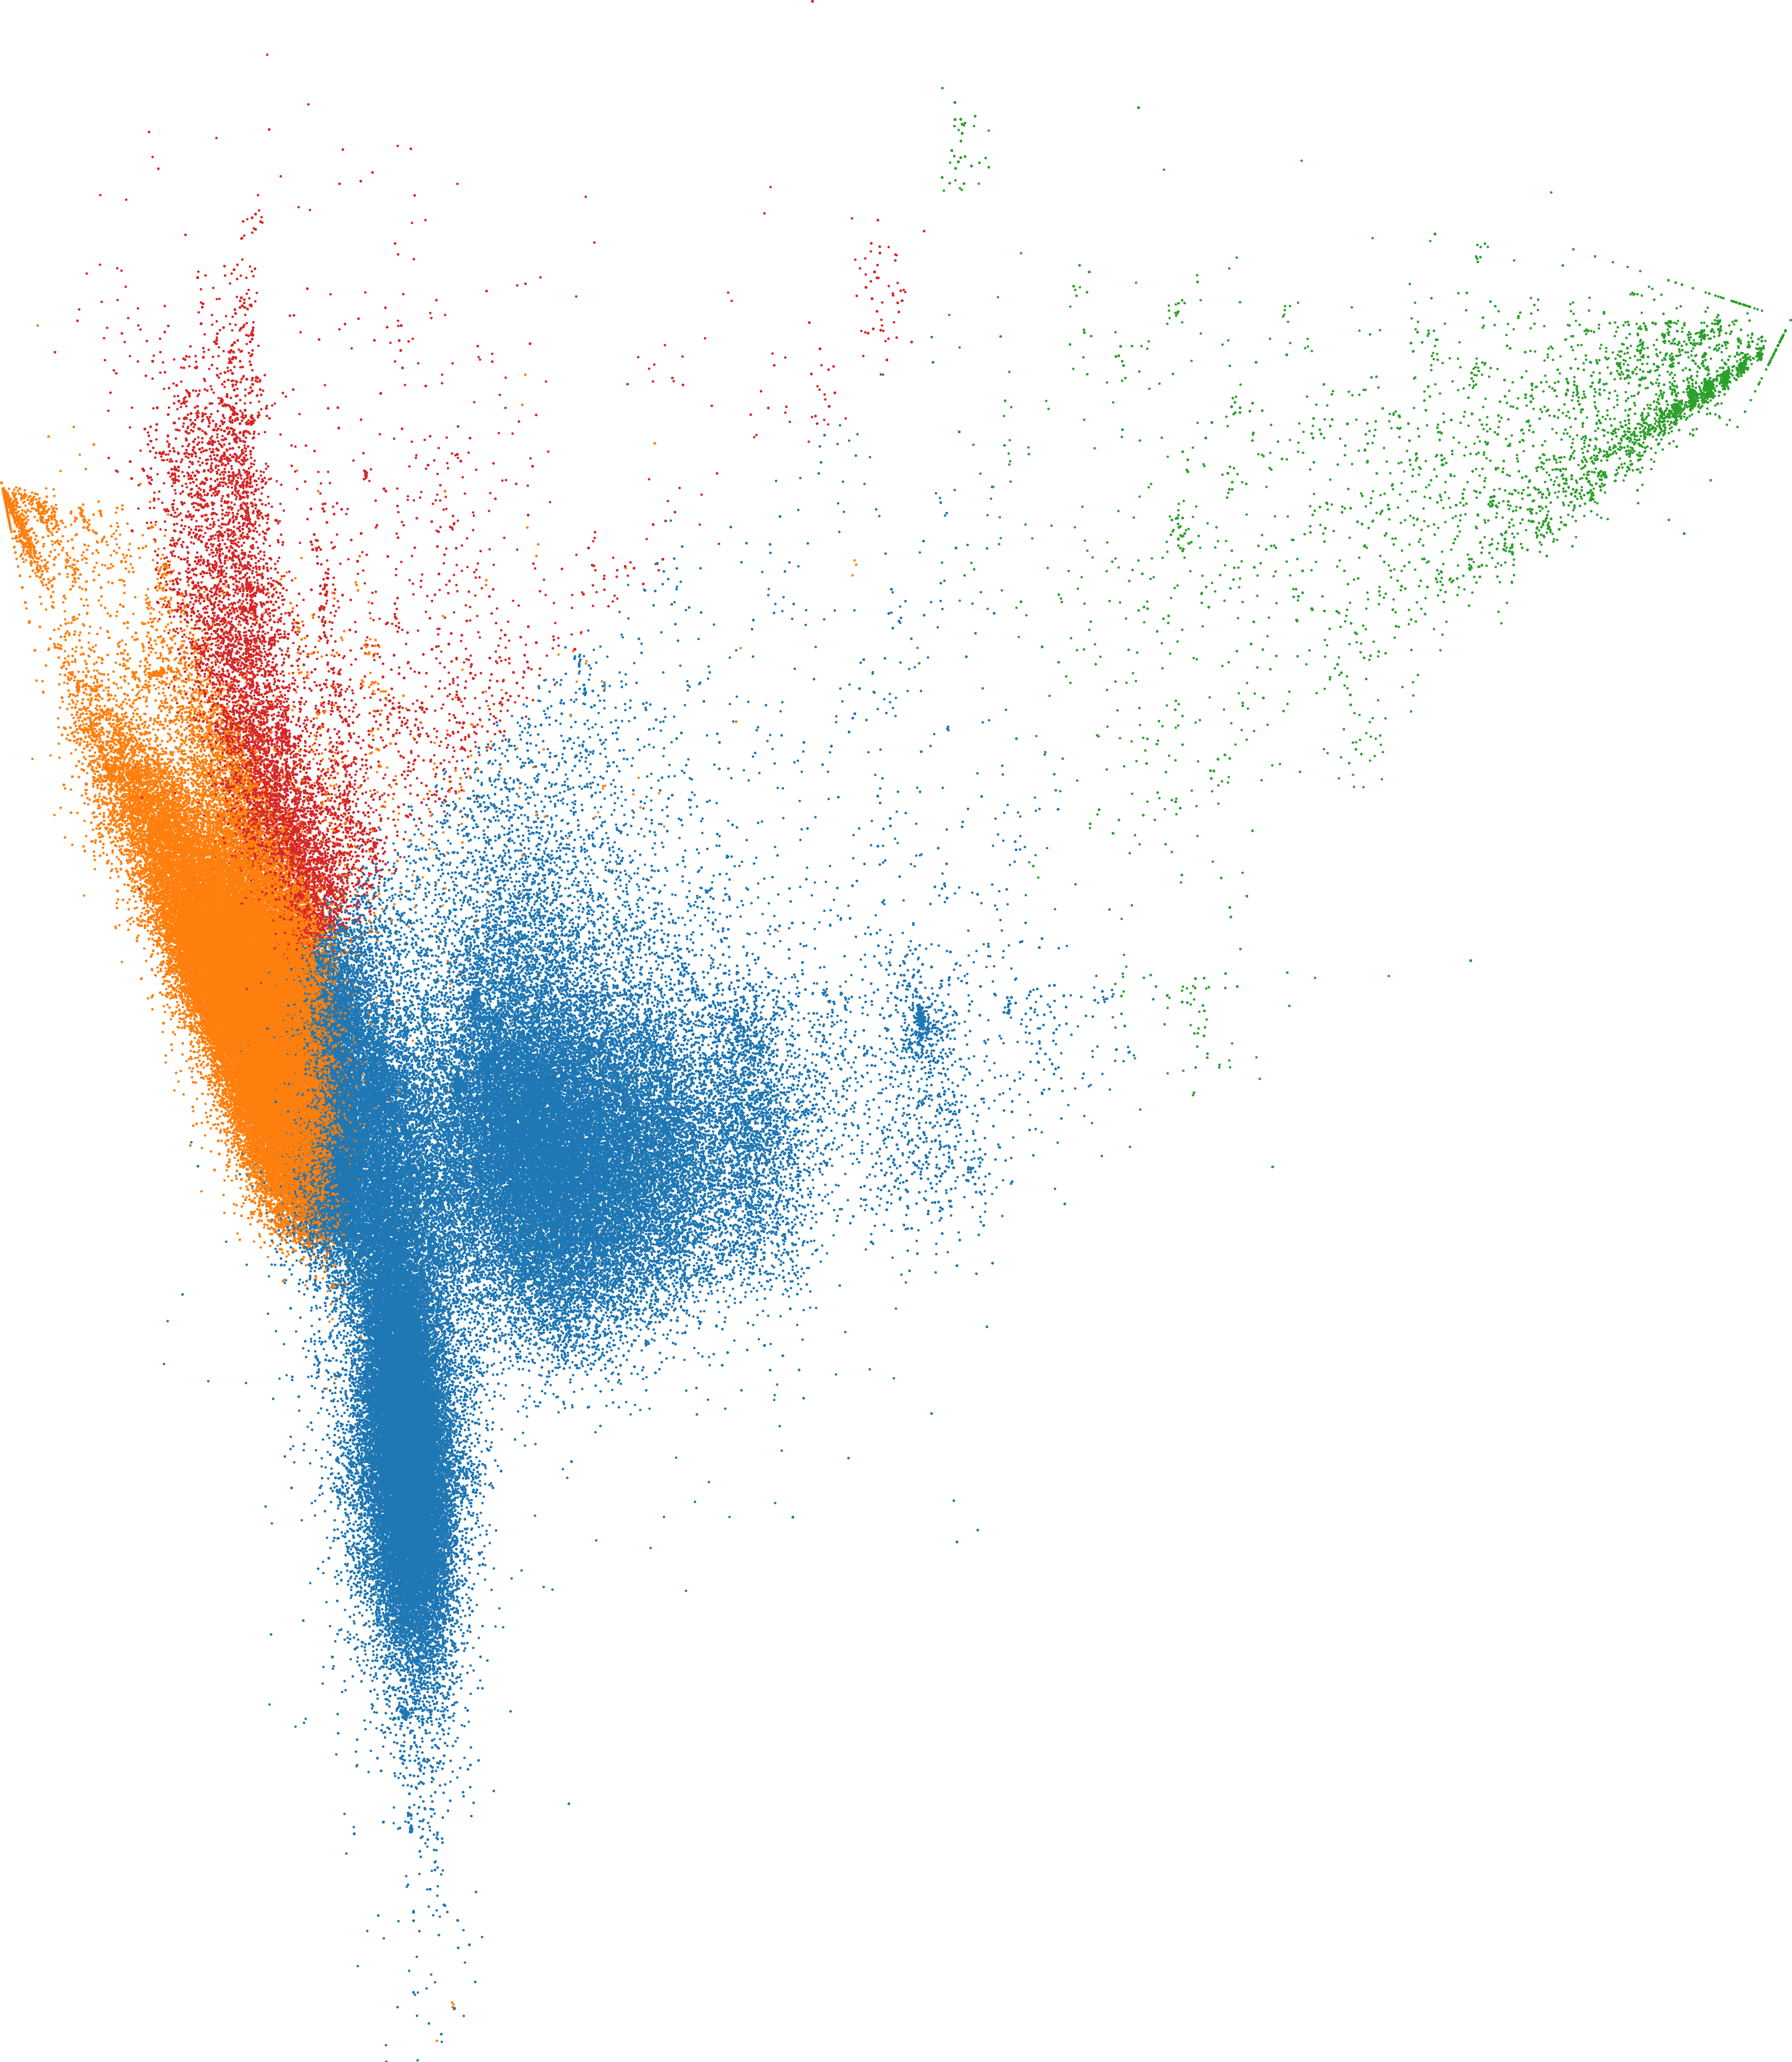
\includegraphics[interpolate=true,width=3.174167in,height=3.652500in]{figures/2d_cluster_marginals-img0.png}}%
\end{pgfscope}%
\begin{pgfscope}%
\pgfpathrectangle{\pgfqpoint{0.692593in}{0.499691in}}{\pgfqpoint{3.617974in}{3.662560in}}%
\pgfusepath{clip}%
\pgfsetbuttcap%
\pgfsetroundjoin%
\definecolor{currentfill}{rgb}{0.121569,0.466667,0.705882}%
\pgfsetfillcolor{currentfill}%
\pgfsetlinewidth{1.003750pt}%
\definecolor{currentstroke}{rgb}{0.121569,0.466667,0.705882}%
\pgfsetstrokecolor{currentstroke}%
\pgfsetdash{}{0pt}%
\pgfsys@defobject{currentmarker}{\pgfqpoint{-0.041667in}{-0.041667in}}{\pgfqpoint{0.041667in}{0.041667in}}{%
\pgfpathmoveto{\pgfqpoint{0.000000in}{-0.041667in}}%
\pgfpathcurveto{\pgfqpoint{0.011050in}{-0.041667in}}{\pgfqpoint{0.021649in}{-0.037276in}}{\pgfqpoint{0.029463in}{-0.029463in}}%
\pgfpathcurveto{\pgfqpoint{0.037276in}{-0.021649in}}{\pgfqpoint{0.041667in}{-0.011050in}}{\pgfqpoint{0.041667in}{0.000000in}}%
\pgfpathcurveto{\pgfqpoint{0.041667in}{0.011050in}}{\pgfqpoint{0.037276in}{0.021649in}}{\pgfqpoint{0.029463in}{0.029463in}}%
\pgfpathcurveto{\pgfqpoint{0.021649in}{0.037276in}}{\pgfqpoint{0.011050in}{0.041667in}}{\pgfqpoint{0.000000in}{0.041667in}}%
\pgfpathcurveto{\pgfqpoint{-0.011050in}{0.041667in}}{\pgfqpoint{-0.021649in}{0.037276in}}{\pgfqpoint{-0.029463in}{0.029463in}}%
\pgfpathcurveto{\pgfqpoint{-0.037276in}{0.021649in}}{\pgfqpoint{-0.041667in}{0.011050in}}{\pgfqpoint{-0.041667in}{0.000000in}}%
\pgfpathcurveto{\pgfqpoint{-0.041667in}{-0.011050in}}{\pgfqpoint{-0.037276in}{-0.021649in}}{\pgfqpoint{-0.029463in}{-0.029463in}}%
\pgfpathcurveto{\pgfqpoint{-0.021649in}{-0.037276in}}{\pgfqpoint{-0.011050in}{-0.041667in}}{\pgfqpoint{0.000000in}{-0.041667in}}%
\pgfpathclose%
\pgfusepath{stroke,fill}%
}%
\end{pgfscope}%
\begin{pgfscope}%
\pgfpathrectangle{\pgfqpoint{0.692593in}{0.499691in}}{\pgfqpoint{3.617974in}{3.662560in}}%
\pgfusepath{clip}%
\pgfsetbuttcap%
\pgfsetroundjoin%
\definecolor{currentfill}{rgb}{1.000000,0.498039,0.054902}%
\pgfsetfillcolor{currentfill}%
\pgfsetlinewidth{1.003750pt}%
\definecolor{currentstroke}{rgb}{1.000000,0.498039,0.054902}%
\pgfsetstrokecolor{currentstroke}%
\pgfsetdash{}{0pt}%
\pgfsys@defobject{currentmarker}{\pgfqpoint{-0.041667in}{-0.041667in}}{\pgfqpoint{0.041667in}{0.041667in}}{%
\pgfpathmoveto{\pgfqpoint{0.000000in}{-0.041667in}}%
\pgfpathcurveto{\pgfqpoint{0.011050in}{-0.041667in}}{\pgfqpoint{0.021649in}{-0.037276in}}{\pgfqpoint{0.029463in}{-0.029463in}}%
\pgfpathcurveto{\pgfqpoint{0.037276in}{-0.021649in}}{\pgfqpoint{0.041667in}{-0.011050in}}{\pgfqpoint{0.041667in}{0.000000in}}%
\pgfpathcurveto{\pgfqpoint{0.041667in}{0.011050in}}{\pgfqpoint{0.037276in}{0.021649in}}{\pgfqpoint{0.029463in}{0.029463in}}%
\pgfpathcurveto{\pgfqpoint{0.021649in}{0.037276in}}{\pgfqpoint{0.011050in}{0.041667in}}{\pgfqpoint{0.000000in}{0.041667in}}%
\pgfpathcurveto{\pgfqpoint{-0.011050in}{0.041667in}}{\pgfqpoint{-0.021649in}{0.037276in}}{\pgfqpoint{-0.029463in}{0.029463in}}%
\pgfpathcurveto{\pgfqpoint{-0.037276in}{0.021649in}}{\pgfqpoint{-0.041667in}{0.011050in}}{\pgfqpoint{-0.041667in}{0.000000in}}%
\pgfpathcurveto{\pgfqpoint{-0.041667in}{-0.011050in}}{\pgfqpoint{-0.037276in}{-0.021649in}}{\pgfqpoint{-0.029463in}{-0.029463in}}%
\pgfpathcurveto{\pgfqpoint{-0.021649in}{-0.037276in}}{\pgfqpoint{-0.011050in}{-0.041667in}}{\pgfqpoint{0.000000in}{-0.041667in}}%
\pgfpathclose%
\pgfusepath{stroke,fill}%
}%
\end{pgfscope}%
\begin{pgfscope}%
\pgfpathrectangle{\pgfqpoint{0.692593in}{0.499691in}}{\pgfqpoint{3.617974in}{3.662560in}}%
\pgfusepath{clip}%
\pgfsetbuttcap%
\pgfsetroundjoin%
\definecolor{currentfill}{rgb}{0.172549,0.627451,0.172549}%
\pgfsetfillcolor{currentfill}%
\pgfsetlinewidth{1.003750pt}%
\definecolor{currentstroke}{rgb}{0.172549,0.627451,0.172549}%
\pgfsetstrokecolor{currentstroke}%
\pgfsetdash{}{0pt}%
\pgfsys@defobject{currentmarker}{\pgfqpoint{-0.041667in}{-0.041667in}}{\pgfqpoint{0.041667in}{0.041667in}}{%
\pgfpathmoveto{\pgfqpoint{0.000000in}{-0.041667in}}%
\pgfpathcurveto{\pgfqpoint{0.011050in}{-0.041667in}}{\pgfqpoint{0.021649in}{-0.037276in}}{\pgfqpoint{0.029463in}{-0.029463in}}%
\pgfpathcurveto{\pgfqpoint{0.037276in}{-0.021649in}}{\pgfqpoint{0.041667in}{-0.011050in}}{\pgfqpoint{0.041667in}{0.000000in}}%
\pgfpathcurveto{\pgfqpoint{0.041667in}{0.011050in}}{\pgfqpoint{0.037276in}{0.021649in}}{\pgfqpoint{0.029463in}{0.029463in}}%
\pgfpathcurveto{\pgfqpoint{0.021649in}{0.037276in}}{\pgfqpoint{0.011050in}{0.041667in}}{\pgfqpoint{0.000000in}{0.041667in}}%
\pgfpathcurveto{\pgfqpoint{-0.011050in}{0.041667in}}{\pgfqpoint{-0.021649in}{0.037276in}}{\pgfqpoint{-0.029463in}{0.029463in}}%
\pgfpathcurveto{\pgfqpoint{-0.037276in}{0.021649in}}{\pgfqpoint{-0.041667in}{0.011050in}}{\pgfqpoint{-0.041667in}{0.000000in}}%
\pgfpathcurveto{\pgfqpoint{-0.041667in}{-0.011050in}}{\pgfqpoint{-0.037276in}{-0.021649in}}{\pgfqpoint{-0.029463in}{-0.029463in}}%
\pgfpathcurveto{\pgfqpoint{-0.021649in}{-0.037276in}}{\pgfqpoint{-0.011050in}{-0.041667in}}{\pgfqpoint{0.000000in}{-0.041667in}}%
\pgfpathclose%
\pgfusepath{stroke,fill}%
}%
\end{pgfscope}%
\begin{pgfscope}%
\pgfpathrectangle{\pgfqpoint{0.692593in}{0.499691in}}{\pgfqpoint{3.617974in}{3.662560in}}%
\pgfusepath{clip}%
\pgfsetbuttcap%
\pgfsetroundjoin%
\definecolor{currentfill}{rgb}{0.839216,0.152941,0.156863}%
\pgfsetfillcolor{currentfill}%
\pgfsetlinewidth{1.003750pt}%
\definecolor{currentstroke}{rgb}{0.839216,0.152941,0.156863}%
\pgfsetstrokecolor{currentstroke}%
\pgfsetdash{}{0pt}%
\pgfsys@defobject{currentmarker}{\pgfqpoint{-0.041667in}{-0.041667in}}{\pgfqpoint{0.041667in}{0.041667in}}{%
\pgfpathmoveto{\pgfqpoint{0.000000in}{-0.041667in}}%
\pgfpathcurveto{\pgfqpoint{0.011050in}{-0.041667in}}{\pgfqpoint{0.021649in}{-0.037276in}}{\pgfqpoint{0.029463in}{-0.029463in}}%
\pgfpathcurveto{\pgfqpoint{0.037276in}{-0.021649in}}{\pgfqpoint{0.041667in}{-0.011050in}}{\pgfqpoint{0.041667in}{0.000000in}}%
\pgfpathcurveto{\pgfqpoint{0.041667in}{0.011050in}}{\pgfqpoint{0.037276in}{0.021649in}}{\pgfqpoint{0.029463in}{0.029463in}}%
\pgfpathcurveto{\pgfqpoint{0.021649in}{0.037276in}}{\pgfqpoint{0.011050in}{0.041667in}}{\pgfqpoint{0.000000in}{0.041667in}}%
\pgfpathcurveto{\pgfqpoint{-0.011050in}{0.041667in}}{\pgfqpoint{-0.021649in}{0.037276in}}{\pgfqpoint{-0.029463in}{0.029463in}}%
\pgfpathcurveto{\pgfqpoint{-0.037276in}{0.021649in}}{\pgfqpoint{-0.041667in}{0.011050in}}{\pgfqpoint{-0.041667in}{0.000000in}}%
\pgfpathcurveto{\pgfqpoint{-0.041667in}{-0.011050in}}{\pgfqpoint{-0.037276in}{-0.021649in}}{\pgfqpoint{-0.029463in}{-0.029463in}}%
\pgfpathcurveto{\pgfqpoint{-0.021649in}{-0.037276in}}{\pgfqpoint{-0.011050in}{-0.041667in}}{\pgfqpoint{0.000000in}{-0.041667in}}%
\pgfpathclose%
\pgfusepath{stroke,fill}%
}%
\end{pgfscope}%
\begin{pgfscope}%
\pgfpathrectangle{\pgfqpoint{0.692593in}{0.499691in}}{\pgfqpoint{3.617974in}{3.662560in}}%
\pgfusepath{clip}%
\pgfsetbuttcap%
\pgfsetroundjoin%
\definecolor{currentfill}{rgb}{0.000000,0.000000,0.000000}%
\pgfsetfillcolor{currentfill}%
\pgfsetlinewidth{0.000000pt}%
\definecolor{currentstroke}{rgb}{1.000000,1.000000,1.000000}%
\pgfsetstrokecolor{currentstroke}%
\pgfsetdash{}{0pt}%
\pgfsys@defobject{currentmarker}{\pgfqpoint{-0.049105in}{-0.049105in}}{\pgfqpoint{0.049105in}{0.049105in}}{%
\pgfpathmoveto{\pgfqpoint{-0.024552in}{-0.049105in}}%
\pgfpathlineto{\pgfqpoint{0.000000in}{-0.024552in}}%
\pgfpathlineto{\pgfqpoint{0.024552in}{-0.049105in}}%
\pgfpathlineto{\pgfqpoint{0.049105in}{-0.024552in}}%
\pgfpathlineto{\pgfqpoint{0.024552in}{0.000000in}}%
\pgfpathlineto{\pgfqpoint{0.049105in}{0.024552in}}%
\pgfpathlineto{\pgfqpoint{0.024552in}{0.049105in}}%
\pgfpathlineto{\pgfqpoint{0.000000in}{0.024552in}}%
\pgfpathlineto{\pgfqpoint{-0.024552in}{0.049105in}}%
\pgfpathlineto{\pgfqpoint{-0.049105in}{0.024552in}}%
\pgfpathlineto{\pgfqpoint{-0.024552in}{0.000000in}}%
\pgfpathlineto{\pgfqpoint{-0.049105in}{-0.024552in}}%
\pgfpathclose%
\pgfusepath{fill}%
}%
\begin{pgfscope}%
\pgfsys@transformshift{1.709481in}{2.038882in}%
\pgfsys@useobject{currentmarker}{}%
\end{pgfscope}%
\begin{pgfscope}%
\pgfsys@transformshift{1.299571in}{2.489760in}%
\pgfsys@useobject{currentmarker}{}%
\end{pgfscope}%
\begin{pgfscope}%
\pgfsys@transformshift{3.657412in}{3.368882in}%
\pgfsys@useobject{currentmarker}{}%
\end{pgfscope}%
\begin{pgfscope}%
\pgfsys@transformshift{1.296028in}{3.069458in}%
\pgfsys@useobject{currentmarker}{}%
\end{pgfscope}%
\end{pgfscope}%
\begin{pgfscope}%
\pgfpathrectangle{\pgfqpoint{0.692593in}{0.499691in}}{\pgfqpoint{3.617974in}{3.662560in}}%
\pgfusepath{clip}%
\pgfsetrectcap%
\pgfsetroundjoin%
\pgfsetlinewidth{0.803000pt}%
\definecolor{currentstroke}{rgb}{0.690196,0.690196,0.690196}%
\pgfsetstrokecolor{currentstroke}%
\pgfsetdash{}{0pt}%
\pgfpathmoveto{\pgfqpoint{0.815808in}{0.499691in}}%
\pgfpathlineto{\pgfqpoint{0.815808in}{4.162251in}}%
\pgfusepath{stroke}%
\end{pgfscope}%
\begin{pgfscope}%
\pgfsetbuttcap%
\pgfsetroundjoin%
\definecolor{currentfill}{rgb}{0.000000,0.000000,0.000000}%
\pgfsetfillcolor{currentfill}%
\pgfsetlinewidth{0.803000pt}%
\definecolor{currentstroke}{rgb}{0.000000,0.000000,0.000000}%
\pgfsetstrokecolor{currentstroke}%
\pgfsetdash{}{0pt}%
\pgfsys@defobject{currentmarker}{\pgfqpoint{0.000000in}{-0.048611in}}{\pgfqpoint{0.000000in}{0.000000in}}{%
\pgfpathmoveto{\pgfqpoint{0.000000in}{0.000000in}}%
\pgfpathlineto{\pgfqpoint{0.000000in}{-0.048611in}}%
\pgfusepath{stroke,fill}%
}%
\begin{pgfscope}%
\pgfsys@transformshift{0.815808in}{0.499691in}%
\pgfsys@useobject{currentmarker}{}%
\end{pgfscope}%
\end{pgfscope}%
\begin{pgfscope}%
\definecolor{textcolor}{rgb}{0.000000,0.000000,0.000000}%
\pgfsetstrokecolor{textcolor}%
\pgfsetfillcolor{textcolor}%
\pgftext[x=0.815808in,y=0.402469in,,top]{\color{textcolor}\rmfamily\fontsize{10.000000}{12.000000}\selectfont \(\displaystyle {-100}\)}%
\end{pgfscope}%
\begin{pgfscope}%
\pgfpathrectangle{\pgfqpoint{0.692593in}{0.499691in}}{\pgfqpoint{3.617974in}{3.662560in}}%
\pgfusepath{clip}%
\pgfsetrectcap%
\pgfsetroundjoin%
\pgfsetlinewidth{0.803000pt}%
\definecolor{currentstroke}{rgb}{0.690196,0.690196,0.690196}%
\pgfsetstrokecolor{currentstroke}%
\pgfsetdash{}{0pt}%
\pgfpathmoveto{\pgfqpoint{1.477714in}{0.499691in}}%
\pgfpathlineto{\pgfqpoint{1.477714in}{4.162251in}}%
\pgfusepath{stroke}%
\end{pgfscope}%
\begin{pgfscope}%
\pgfsetbuttcap%
\pgfsetroundjoin%
\definecolor{currentfill}{rgb}{0.000000,0.000000,0.000000}%
\pgfsetfillcolor{currentfill}%
\pgfsetlinewidth{0.803000pt}%
\definecolor{currentstroke}{rgb}{0.000000,0.000000,0.000000}%
\pgfsetstrokecolor{currentstroke}%
\pgfsetdash{}{0pt}%
\pgfsys@defobject{currentmarker}{\pgfqpoint{0.000000in}{-0.048611in}}{\pgfqpoint{0.000000in}{0.000000in}}{%
\pgfpathmoveto{\pgfqpoint{0.000000in}{0.000000in}}%
\pgfpathlineto{\pgfqpoint{0.000000in}{-0.048611in}}%
\pgfusepath{stroke,fill}%
}%
\begin{pgfscope}%
\pgfsys@transformshift{1.477714in}{0.499691in}%
\pgfsys@useobject{currentmarker}{}%
\end{pgfscope}%
\end{pgfscope}%
\begin{pgfscope}%
\definecolor{textcolor}{rgb}{0.000000,0.000000,0.000000}%
\pgfsetstrokecolor{textcolor}%
\pgfsetfillcolor{textcolor}%
\pgftext[x=1.477714in,y=0.402469in,,top]{\color{textcolor}\rmfamily\fontsize{10.000000}{12.000000}\selectfont \(\displaystyle {0}\)}%
\end{pgfscope}%
\begin{pgfscope}%
\pgfpathrectangle{\pgfqpoint{0.692593in}{0.499691in}}{\pgfqpoint{3.617974in}{3.662560in}}%
\pgfusepath{clip}%
\pgfsetrectcap%
\pgfsetroundjoin%
\pgfsetlinewidth{0.803000pt}%
\definecolor{currentstroke}{rgb}{0.690196,0.690196,0.690196}%
\pgfsetstrokecolor{currentstroke}%
\pgfsetdash{}{0pt}%
\pgfpathmoveto{\pgfqpoint{2.139620in}{0.499691in}}%
\pgfpathlineto{\pgfqpoint{2.139620in}{4.162251in}}%
\pgfusepath{stroke}%
\end{pgfscope}%
\begin{pgfscope}%
\pgfsetbuttcap%
\pgfsetroundjoin%
\definecolor{currentfill}{rgb}{0.000000,0.000000,0.000000}%
\pgfsetfillcolor{currentfill}%
\pgfsetlinewidth{0.803000pt}%
\definecolor{currentstroke}{rgb}{0.000000,0.000000,0.000000}%
\pgfsetstrokecolor{currentstroke}%
\pgfsetdash{}{0pt}%
\pgfsys@defobject{currentmarker}{\pgfqpoint{0.000000in}{-0.048611in}}{\pgfqpoint{0.000000in}{0.000000in}}{%
\pgfpathmoveto{\pgfqpoint{0.000000in}{0.000000in}}%
\pgfpathlineto{\pgfqpoint{0.000000in}{-0.048611in}}%
\pgfusepath{stroke,fill}%
}%
\begin{pgfscope}%
\pgfsys@transformshift{2.139620in}{0.499691in}%
\pgfsys@useobject{currentmarker}{}%
\end{pgfscope}%
\end{pgfscope}%
\begin{pgfscope}%
\definecolor{textcolor}{rgb}{0.000000,0.000000,0.000000}%
\pgfsetstrokecolor{textcolor}%
\pgfsetfillcolor{textcolor}%
\pgftext[x=2.139620in,y=0.402469in,,top]{\color{textcolor}\rmfamily\fontsize{10.000000}{12.000000}\selectfont \(\displaystyle {100}\)}%
\end{pgfscope}%
\begin{pgfscope}%
\pgfpathrectangle{\pgfqpoint{0.692593in}{0.499691in}}{\pgfqpoint{3.617974in}{3.662560in}}%
\pgfusepath{clip}%
\pgfsetrectcap%
\pgfsetroundjoin%
\pgfsetlinewidth{0.803000pt}%
\definecolor{currentstroke}{rgb}{0.690196,0.690196,0.690196}%
\pgfsetstrokecolor{currentstroke}%
\pgfsetdash{}{0pt}%
\pgfpathmoveto{\pgfqpoint{2.801526in}{0.499691in}}%
\pgfpathlineto{\pgfqpoint{2.801526in}{4.162251in}}%
\pgfusepath{stroke}%
\end{pgfscope}%
\begin{pgfscope}%
\pgfsetbuttcap%
\pgfsetroundjoin%
\definecolor{currentfill}{rgb}{0.000000,0.000000,0.000000}%
\pgfsetfillcolor{currentfill}%
\pgfsetlinewidth{0.803000pt}%
\definecolor{currentstroke}{rgb}{0.000000,0.000000,0.000000}%
\pgfsetstrokecolor{currentstroke}%
\pgfsetdash{}{0pt}%
\pgfsys@defobject{currentmarker}{\pgfqpoint{0.000000in}{-0.048611in}}{\pgfqpoint{0.000000in}{0.000000in}}{%
\pgfpathmoveto{\pgfqpoint{0.000000in}{0.000000in}}%
\pgfpathlineto{\pgfqpoint{0.000000in}{-0.048611in}}%
\pgfusepath{stroke,fill}%
}%
\begin{pgfscope}%
\pgfsys@transformshift{2.801526in}{0.499691in}%
\pgfsys@useobject{currentmarker}{}%
\end{pgfscope}%
\end{pgfscope}%
\begin{pgfscope}%
\definecolor{textcolor}{rgb}{0.000000,0.000000,0.000000}%
\pgfsetstrokecolor{textcolor}%
\pgfsetfillcolor{textcolor}%
\pgftext[x=2.801526in,y=0.402469in,,top]{\color{textcolor}\rmfamily\fontsize{10.000000}{12.000000}\selectfont \(\displaystyle {200}\)}%
\end{pgfscope}%
\begin{pgfscope}%
\pgfpathrectangle{\pgfqpoint{0.692593in}{0.499691in}}{\pgfqpoint{3.617974in}{3.662560in}}%
\pgfusepath{clip}%
\pgfsetrectcap%
\pgfsetroundjoin%
\pgfsetlinewidth{0.803000pt}%
\definecolor{currentstroke}{rgb}{0.690196,0.690196,0.690196}%
\pgfsetstrokecolor{currentstroke}%
\pgfsetdash{}{0pt}%
\pgfpathmoveto{\pgfqpoint{3.463432in}{0.499691in}}%
\pgfpathlineto{\pgfqpoint{3.463432in}{4.162251in}}%
\pgfusepath{stroke}%
\end{pgfscope}%
\begin{pgfscope}%
\pgfsetbuttcap%
\pgfsetroundjoin%
\definecolor{currentfill}{rgb}{0.000000,0.000000,0.000000}%
\pgfsetfillcolor{currentfill}%
\pgfsetlinewidth{0.803000pt}%
\definecolor{currentstroke}{rgb}{0.000000,0.000000,0.000000}%
\pgfsetstrokecolor{currentstroke}%
\pgfsetdash{}{0pt}%
\pgfsys@defobject{currentmarker}{\pgfqpoint{0.000000in}{-0.048611in}}{\pgfqpoint{0.000000in}{0.000000in}}{%
\pgfpathmoveto{\pgfqpoint{0.000000in}{0.000000in}}%
\pgfpathlineto{\pgfqpoint{0.000000in}{-0.048611in}}%
\pgfusepath{stroke,fill}%
}%
\begin{pgfscope}%
\pgfsys@transformshift{3.463432in}{0.499691in}%
\pgfsys@useobject{currentmarker}{}%
\end{pgfscope}%
\end{pgfscope}%
\begin{pgfscope}%
\definecolor{textcolor}{rgb}{0.000000,0.000000,0.000000}%
\pgfsetstrokecolor{textcolor}%
\pgfsetfillcolor{textcolor}%
\pgftext[x=3.463432in,y=0.402469in,,top]{\color{textcolor}\rmfamily\fontsize{10.000000}{12.000000}\selectfont \(\displaystyle {300}\)}%
\end{pgfscope}%
\begin{pgfscope}%
\pgfpathrectangle{\pgfqpoint{0.692593in}{0.499691in}}{\pgfqpoint{3.617974in}{3.662560in}}%
\pgfusepath{clip}%
\pgfsetrectcap%
\pgfsetroundjoin%
\pgfsetlinewidth{0.803000pt}%
\definecolor{currentstroke}{rgb}{0.690196,0.690196,0.690196}%
\pgfsetstrokecolor{currentstroke}%
\pgfsetdash{}{0pt}%
\pgfpathmoveto{\pgfqpoint{4.125338in}{0.499691in}}%
\pgfpathlineto{\pgfqpoint{4.125338in}{4.162251in}}%
\pgfusepath{stroke}%
\end{pgfscope}%
\begin{pgfscope}%
\pgfsetbuttcap%
\pgfsetroundjoin%
\definecolor{currentfill}{rgb}{0.000000,0.000000,0.000000}%
\pgfsetfillcolor{currentfill}%
\pgfsetlinewidth{0.803000pt}%
\definecolor{currentstroke}{rgb}{0.000000,0.000000,0.000000}%
\pgfsetstrokecolor{currentstroke}%
\pgfsetdash{}{0pt}%
\pgfsys@defobject{currentmarker}{\pgfqpoint{0.000000in}{-0.048611in}}{\pgfqpoint{0.000000in}{0.000000in}}{%
\pgfpathmoveto{\pgfqpoint{0.000000in}{0.000000in}}%
\pgfpathlineto{\pgfqpoint{0.000000in}{-0.048611in}}%
\pgfusepath{stroke,fill}%
}%
\begin{pgfscope}%
\pgfsys@transformshift{4.125338in}{0.499691in}%
\pgfsys@useobject{currentmarker}{}%
\end{pgfscope}%
\end{pgfscope}%
\begin{pgfscope}%
\definecolor{textcolor}{rgb}{0.000000,0.000000,0.000000}%
\pgfsetstrokecolor{textcolor}%
\pgfsetfillcolor{textcolor}%
\pgftext[x=4.125338in,y=0.402469in,,top]{\color{textcolor}\rmfamily\fontsize{10.000000}{12.000000}\selectfont \(\displaystyle {400}\)}%
\end{pgfscope}%
\begin{pgfscope}%
\definecolor{textcolor}{rgb}{0.000000,0.000000,0.000000}%
\pgfsetstrokecolor{textcolor}%
\pgfsetfillcolor{textcolor}%
\pgftext[x=2.501580in,y=0.223457in,,top]{\color{textcolor}\rmfamily\fontsize{10.000000}{12.000000}\selectfont PC1}%
\end{pgfscope}%
\begin{pgfscope}%
\pgfpathrectangle{\pgfqpoint{0.692593in}{0.499691in}}{\pgfqpoint{3.617974in}{3.662560in}}%
\pgfusepath{clip}%
\pgfsetrectcap%
\pgfsetroundjoin%
\pgfsetlinewidth{0.803000pt}%
\definecolor{currentstroke}{rgb}{0.690196,0.690196,0.690196}%
\pgfsetstrokecolor{currentstroke}%
\pgfsetdash{}{0pt}%
\pgfpathmoveto{\pgfqpoint{0.692593in}{0.499691in}}%
\pgfpathlineto{\pgfqpoint{4.310567in}{0.499691in}}%
\pgfusepath{stroke}%
\end{pgfscope}%
\begin{pgfscope}%
\pgfsetbuttcap%
\pgfsetroundjoin%
\definecolor{currentfill}{rgb}{0.000000,0.000000,0.000000}%
\pgfsetfillcolor{currentfill}%
\pgfsetlinewidth{0.803000pt}%
\definecolor{currentstroke}{rgb}{0.000000,0.000000,0.000000}%
\pgfsetstrokecolor{currentstroke}%
\pgfsetdash{}{0pt}%
\pgfsys@defobject{currentmarker}{\pgfqpoint{-0.048611in}{0.000000in}}{\pgfqpoint{0.000000in}{0.000000in}}{%
\pgfpathmoveto{\pgfqpoint{0.000000in}{0.000000in}}%
\pgfpathlineto{\pgfqpoint{-0.048611in}{0.000000in}}%
\pgfusepath{stroke,fill}%
}%
\begin{pgfscope}%
\pgfsys@transformshift{0.692593in}{0.499691in}%
\pgfsys@useobject{currentmarker}{}%
\end{pgfscope}%
\end{pgfscope}%
\begin{pgfscope}%
\definecolor{textcolor}{rgb}{0.000000,0.000000,0.000000}%
\pgfsetstrokecolor{textcolor}%
\pgfsetfillcolor{textcolor}%
\pgftext[x=0.279012in, y=0.451466in, left, base]{\color{textcolor}\rmfamily\fontsize{10.000000}{12.000000}\selectfont \(\displaystyle {-200}\)}%
\end{pgfscope}%
\begin{pgfscope}%
\pgfpathrectangle{\pgfqpoint{0.692593in}{0.499691in}}{\pgfqpoint{3.617974in}{3.662560in}}%
\pgfusepath{clip}%
\pgfsetrectcap%
\pgfsetroundjoin%
\pgfsetlinewidth{0.803000pt}%
\definecolor{currentstroke}{rgb}{0.690196,0.690196,0.690196}%
\pgfsetstrokecolor{currentstroke}%
\pgfsetdash{}{0pt}%
\pgfpathmoveto{\pgfqpoint{0.692593in}{1.022914in}}%
\pgfpathlineto{\pgfqpoint{4.310567in}{1.022914in}}%
\pgfusepath{stroke}%
\end{pgfscope}%
\begin{pgfscope}%
\pgfsetbuttcap%
\pgfsetroundjoin%
\definecolor{currentfill}{rgb}{0.000000,0.000000,0.000000}%
\pgfsetfillcolor{currentfill}%
\pgfsetlinewidth{0.803000pt}%
\definecolor{currentstroke}{rgb}{0.000000,0.000000,0.000000}%
\pgfsetstrokecolor{currentstroke}%
\pgfsetdash{}{0pt}%
\pgfsys@defobject{currentmarker}{\pgfqpoint{-0.048611in}{0.000000in}}{\pgfqpoint{0.000000in}{0.000000in}}{%
\pgfpathmoveto{\pgfqpoint{0.000000in}{0.000000in}}%
\pgfpathlineto{\pgfqpoint{-0.048611in}{0.000000in}}%
\pgfusepath{stroke,fill}%
}%
\begin{pgfscope}%
\pgfsys@transformshift{0.692593in}{1.022914in}%
\pgfsys@useobject{currentmarker}{}%
\end{pgfscope}%
\end{pgfscope}%
\begin{pgfscope}%
\definecolor{textcolor}{rgb}{0.000000,0.000000,0.000000}%
\pgfsetstrokecolor{textcolor}%
\pgfsetfillcolor{textcolor}%
\pgftext[x=0.279012in, y=0.974689in, left, base]{\color{textcolor}\rmfamily\fontsize{10.000000}{12.000000}\selectfont \(\displaystyle {-150}\)}%
\end{pgfscope}%
\begin{pgfscope}%
\pgfpathrectangle{\pgfqpoint{0.692593in}{0.499691in}}{\pgfqpoint{3.617974in}{3.662560in}}%
\pgfusepath{clip}%
\pgfsetrectcap%
\pgfsetroundjoin%
\pgfsetlinewidth{0.803000pt}%
\definecolor{currentstroke}{rgb}{0.690196,0.690196,0.690196}%
\pgfsetstrokecolor{currentstroke}%
\pgfsetdash{}{0pt}%
\pgfpathmoveto{\pgfqpoint{0.692593in}{1.546137in}}%
\pgfpathlineto{\pgfqpoint{4.310567in}{1.546137in}}%
\pgfusepath{stroke}%
\end{pgfscope}%
\begin{pgfscope}%
\pgfsetbuttcap%
\pgfsetroundjoin%
\definecolor{currentfill}{rgb}{0.000000,0.000000,0.000000}%
\pgfsetfillcolor{currentfill}%
\pgfsetlinewidth{0.803000pt}%
\definecolor{currentstroke}{rgb}{0.000000,0.000000,0.000000}%
\pgfsetstrokecolor{currentstroke}%
\pgfsetdash{}{0pt}%
\pgfsys@defobject{currentmarker}{\pgfqpoint{-0.048611in}{0.000000in}}{\pgfqpoint{0.000000in}{0.000000in}}{%
\pgfpathmoveto{\pgfqpoint{0.000000in}{0.000000in}}%
\pgfpathlineto{\pgfqpoint{-0.048611in}{0.000000in}}%
\pgfusepath{stroke,fill}%
}%
\begin{pgfscope}%
\pgfsys@transformshift{0.692593in}{1.546137in}%
\pgfsys@useobject{currentmarker}{}%
\end{pgfscope}%
\end{pgfscope}%
\begin{pgfscope}%
\definecolor{textcolor}{rgb}{0.000000,0.000000,0.000000}%
\pgfsetstrokecolor{textcolor}%
\pgfsetfillcolor{textcolor}%
\pgftext[x=0.279012in, y=1.497912in, left, base]{\color{textcolor}\rmfamily\fontsize{10.000000}{12.000000}\selectfont \(\displaystyle {-100}\)}%
\end{pgfscope}%
\begin{pgfscope}%
\pgfpathrectangle{\pgfqpoint{0.692593in}{0.499691in}}{\pgfqpoint{3.617974in}{3.662560in}}%
\pgfusepath{clip}%
\pgfsetrectcap%
\pgfsetroundjoin%
\pgfsetlinewidth{0.803000pt}%
\definecolor{currentstroke}{rgb}{0.690196,0.690196,0.690196}%
\pgfsetstrokecolor{currentstroke}%
\pgfsetdash{}{0pt}%
\pgfpathmoveto{\pgfqpoint{0.692593in}{2.069360in}}%
\pgfpathlineto{\pgfqpoint{4.310567in}{2.069360in}}%
\pgfusepath{stroke}%
\end{pgfscope}%
\begin{pgfscope}%
\pgfsetbuttcap%
\pgfsetroundjoin%
\definecolor{currentfill}{rgb}{0.000000,0.000000,0.000000}%
\pgfsetfillcolor{currentfill}%
\pgfsetlinewidth{0.803000pt}%
\definecolor{currentstroke}{rgb}{0.000000,0.000000,0.000000}%
\pgfsetstrokecolor{currentstroke}%
\pgfsetdash{}{0pt}%
\pgfsys@defobject{currentmarker}{\pgfqpoint{-0.048611in}{0.000000in}}{\pgfqpoint{0.000000in}{0.000000in}}{%
\pgfpathmoveto{\pgfqpoint{0.000000in}{0.000000in}}%
\pgfpathlineto{\pgfqpoint{-0.048611in}{0.000000in}}%
\pgfusepath{stroke,fill}%
}%
\begin{pgfscope}%
\pgfsys@transformshift{0.692593in}{2.069360in}%
\pgfsys@useobject{currentmarker}{}%
\end{pgfscope}%
\end{pgfscope}%
\begin{pgfscope}%
\definecolor{textcolor}{rgb}{0.000000,0.000000,0.000000}%
\pgfsetstrokecolor{textcolor}%
\pgfsetfillcolor{textcolor}%
\pgftext[x=0.348457in, y=2.021134in, left, base]{\color{textcolor}\rmfamily\fontsize{10.000000}{12.000000}\selectfont \(\displaystyle {-50}\)}%
\end{pgfscope}%
\begin{pgfscope}%
\pgfpathrectangle{\pgfqpoint{0.692593in}{0.499691in}}{\pgfqpoint{3.617974in}{3.662560in}}%
\pgfusepath{clip}%
\pgfsetrectcap%
\pgfsetroundjoin%
\pgfsetlinewidth{0.803000pt}%
\definecolor{currentstroke}{rgb}{0.690196,0.690196,0.690196}%
\pgfsetstrokecolor{currentstroke}%
\pgfsetdash{}{0pt}%
\pgfpathmoveto{\pgfqpoint{0.692593in}{2.592583in}}%
\pgfpathlineto{\pgfqpoint{4.310567in}{2.592583in}}%
\pgfusepath{stroke}%
\end{pgfscope}%
\begin{pgfscope}%
\pgfsetbuttcap%
\pgfsetroundjoin%
\definecolor{currentfill}{rgb}{0.000000,0.000000,0.000000}%
\pgfsetfillcolor{currentfill}%
\pgfsetlinewidth{0.803000pt}%
\definecolor{currentstroke}{rgb}{0.000000,0.000000,0.000000}%
\pgfsetstrokecolor{currentstroke}%
\pgfsetdash{}{0pt}%
\pgfsys@defobject{currentmarker}{\pgfqpoint{-0.048611in}{0.000000in}}{\pgfqpoint{0.000000in}{0.000000in}}{%
\pgfpathmoveto{\pgfqpoint{0.000000in}{0.000000in}}%
\pgfpathlineto{\pgfqpoint{-0.048611in}{0.000000in}}%
\pgfusepath{stroke,fill}%
}%
\begin{pgfscope}%
\pgfsys@transformshift{0.692593in}{2.592583in}%
\pgfsys@useobject{currentmarker}{}%
\end{pgfscope}%
\end{pgfscope}%
\begin{pgfscope}%
\definecolor{textcolor}{rgb}{0.000000,0.000000,0.000000}%
\pgfsetstrokecolor{textcolor}%
\pgfsetfillcolor{textcolor}%
\pgftext[x=0.525927in, y=2.544357in, left, base]{\color{textcolor}\rmfamily\fontsize{10.000000}{12.000000}\selectfont \(\displaystyle {0}\)}%
\end{pgfscope}%
\begin{pgfscope}%
\pgfpathrectangle{\pgfqpoint{0.692593in}{0.499691in}}{\pgfqpoint{3.617974in}{3.662560in}}%
\pgfusepath{clip}%
\pgfsetrectcap%
\pgfsetroundjoin%
\pgfsetlinewidth{0.803000pt}%
\definecolor{currentstroke}{rgb}{0.690196,0.690196,0.690196}%
\pgfsetstrokecolor{currentstroke}%
\pgfsetdash{}{0pt}%
\pgfpathmoveto{\pgfqpoint{0.692593in}{3.115805in}}%
\pgfpathlineto{\pgfqpoint{4.310567in}{3.115805in}}%
\pgfusepath{stroke}%
\end{pgfscope}%
\begin{pgfscope}%
\pgfsetbuttcap%
\pgfsetroundjoin%
\definecolor{currentfill}{rgb}{0.000000,0.000000,0.000000}%
\pgfsetfillcolor{currentfill}%
\pgfsetlinewidth{0.803000pt}%
\definecolor{currentstroke}{rgb}{0.000000,0.000000,0.000000}%
\pgfsetstrokecolor{currentstroke}%
\pgfsetdash{}{0pt}%
\pgfsys@defobject{currentmarker}{\pgfqpoint{-0.048611in}{0.000000in}}{\pgfqpoint{0.000000in}{0.000000in}}{%
\pgfpathmoveto{\pgfqpoint{0.000000in}{0.000000in}}%
\pgfpathlineto{\pgfqpoint{-0.048611in}{0.000000in}}%
\pgfusepath{stroke,fill}%
}%
\begin{pgfscope}%
\pgfsys@transformshift{0.692593in}{3.115805in}%
\pgfsys@useobject{currentmarker}{}%
\end{pgfscope}%
\end{pgfscope}%
\begin{pgfscope}%
\definecolor{textcolor}{rgb}{0.000000,0.000000,0.000000}%
\pgfsetstrokecolor{textcolor}%
\pgfsetfillcolor{textcolor}%
\pgftext[x=0.456482in, y=3.067580in, left, base]{\color{textcolor}\rmfamily\fontsize{10.000000}{12.000000}\selectfont \(\displaystyle {50}\)}%
\end{pgfscope}%
\begin{pgfscope}%
\pgfpathrectangle{\pgfqpoint{0.692593in}{0.499691in}}{\pgfqpoint{3.617974in}{3.662560in}}%
\pgfusepath{clip}%
\pgfsetrectcap%
\pgfsetroundjoin%
\pgfsetlinewidth{0.803000pt}%
\definecolor{currentstroke}{rgb}{0.690196,0.690196,0.690196}%
\pgfsetstrokecolor{currentstroke}%
\pgfsetdash{}{0pt}%
\pgfpathmoveto{\pgfqpoint{0.692593in}{3.639028in}}%
\pgfpathlineto{\pgfqpoint{4.310567in}{3.639028in}}%
\pgfusepath{stroke}%
\end{pgfscope}%
\begin{pgfscope}%
\pgfsetbuttcap%
\pgfsetroundjoin%
\definecolor{currentfill}{rgb}{0.000000,0.000000,0.000000}%
\pgfsetfillcolor{currentfill}%
\pgfsetlinewidth{0.803000pt}%
\definecolor{currentstroke}{rgb}{0.000000,0.000000,0.000000}%
\pgfsetstrokecolor{currentstroke}%
\pgfsetdash{}{0pt}%
\pgfsys@defobject{currentmarker}{\pgfqpoint{-0.048611in}{0.000000in}}{\pgfqpoint{0.000000in}{0.000000in}}{%
\pgfpathmoveto{\pgfqpoint{0.000000in}{0.000000in}}%
\pgfpathlineto{\pgfqpoint{-0.048611in}{0.000000in}}%
\pgfusepath{stroke,fill}%
}%
\begin{pgfscope}%
\pgfsys@transformshift{0.692593in}{3.639028in}%
\pgfsys@useobject{currentmarker}{}%
\end{pgfscope}%
\end{pgfscope}%
\begin{pgfscope}%
\definecolor{textcolor}{rgb}{0.000000,0.000000,0.000000}%
\pgfsetstrokecolor{textcolor}%
\pgfsetfillcolor{textcolor}%
\pgftext[x=0.387037in, y=3.590803in, left, base]{\color{textcolor}\rmfamily\fontsize{10.000000}{12.000000}\selectfont \(\displaystyle {100}\)}%
\end{pgfscope}%
\begin{pgfscope}%
\pgfpathrectangle{\pgfqpoint{0.692593in}{0.499691in}}{\pgfqpoint{3.617974in}{3.662560in}}%
\pgfusepath{clip}%
\pgfsetrectcap%
\pgfsetroundjoin%
\pgfsetlinewidth{0.803000pt}%
\definecolor{currentstroke}{rgb}{0.690196,0.690196,0.690196}%
\pgfsetstrokecolor{currentstroke}%
\pgfsetdash{}{0pt}%
\pgfpathmoveto{\pgfqpoint{0.692593in}{4.162251in}}%
\pgfpathlineto{\pgfqpoint{4.310567in}{4.162251in}}%
\pgfusepath{stroke}%
\end{pgfscope}%
\begin{pgfscope}%
\pgfsetbuttcap%
\pgfsetroundjoin%
\definecolor{currentfill}{rgb}{0.000000,0.000000,0.000000}%
\pgfsetfillcolor{currentfill}%
\pgfsetlinewidth{0.803000pt}%
\definecolor{currentstroke}{rgb}{0.000000,0.000000,0.000000}%
\pgfsetstrokecolor{currentstroke}%
\pgfsetdash{}{0pt}%
\pgfsys@defobject{currentmarker}{\pgfqpoint{-0.048611in}{0.000000in}}{\pgfqpoint{0.000000in}{0.000000in}}{%
\pgfpathmoveto{\pgfqpoint{0.000000in}{0.000000in}}%
\pgfpathlineto{\pgfqpoint{-0.048611in}{0.000000in}}%
\pgfusepath{stroke,fill}%
}%
\begin{pgfscope}%
\pgfsys@transformshift{0.692593in}{4.162251in}%
\pgfsys@useobject{currentmarker}{}%
\end{pgfscope}%
\end{pgfscope}%
\begin{pgfscope}%
\definecolor{textcolor}{rgb}{0.000000,0.000000,0.000000}%
\pgfsetstrokecolor{textcolor}%
\pgfsetfillcolor{textcolor}%
\pgftext[x=0.387037in, y=4.114026in, left, base]{\color{textcolor}\rmfamily\fontsize{10.000000}{12.000000}\selectfont \(\displaystyle {150}\)}%
\end{pgfscope}%
\begin{pgfscope}%
\definecolor{textcolor}{rgb}{0.000000,0.000000,0.000000}%
\pgfsetstrokecolor{textcolor}%
\pgfsetfillcolor{textcolor}%
\pgftext[x=0.223457in,y=2.330971in,,bottom,rotate=90.000000]{\color{textcolor}\rmfamily\fontsize{10.000000}{12.000000}\selectfont PC2}%
\end{pgfscope}%
\begin{pgfscope}%
\pgfsetrectcap%
\pgfsetmiterjoin%
\pgfsetlinewidth{0.803000pt}%
\definecolor{currentstroke}{rgb}{0.000000,0.000000,0.000000}%
\pgfsetstrokecolor{currentstroke}%
\pgfsetdash{}{0pt}%
\pgfpathmoveto{\pgfqpoint{0.692593in}{0.499691in}}%
\pgfpathlineto{\pgfqpoint{0.692593in}{4.162251in}}%
\pgfusepath{stroke}%
\end{pgfscope}%
\begin{pgfscope}%
\pgfsetrectcap%
\pgfsetmiterjoin%
\pgfsetlinewidth{0.803000pt}%
\definecolor{currentstroke}{rgb}{0.000000,0.000000,0.000000}%
\pgfsetstrokecolor{currentstroke}%
\pgfsetdash{}{0pt}%
\pgfpathmoveto{\pgfqpoint{0.692593in}{0.499691in}}%
\pgfpathlineto{\pgfqpoint{4.310567in}{0.499691in}}%
\pgfusepath{stroke}%
\end{pgfscope}%
\begin{pgfscope}%
\pgfsetbuttcap%
\pgfsetmiterjoin%
\definecolor{currentfill}{rgb}{1.000000,1.000000,1.000000}%
\pgfsetfillcolor{currentfill}%
\pgfsetfillopacity{0.800000}%
\pgfsetlinewidth{1.003750pt}%
\definecolor{currentstroke}{rgb}{0.800000,0.800000,0.800000}%
\pgfsetstrokecolor{currentstroke}%
\pgfsetstrokeopacity{0.800000}%
\pgfsetdash{}{0pt}%
\pgfpathmoveto{\pgfqpoint{3.212187in}{0.569136in}}%
\pgfpathlineto{\pgfqpoint{4.213345in}{0.569136in}}%
\pgfpathquadraticcurveto{\pgfqpoint{4.241123in}{0.569136in}}{\pgfqpoint{4.241123in}{0.596913in}}%
\pgfpathlineto{\pgfqpoint{4.241123in}{1.551388in}}%
\pgfpathquadraticcurveto{\pgfqpoint{4.241123in}{1.579166in}}{\pgfqpoint{4.213345in}{1.579166in}}%
\pgfpathlineto{\pgfqpoint{3.212187in}{1.579166in}}%
\pgfpathquadraticcurveto{\pgfqpoint{3.184409in}{1.579166in}}{\pgfqpoint{3.184409in}{1.551388in}}%
\pgfpathlineto{\pgfqpoint{3.184409in}{0.596913in}}%
\pgfpathquadraticcurveto{\pgfqpoint{3.184409in}{0.569136in}}{\pgfqpoint{3.212187in}{0.569136in}}%
\pgfpathclose%
\pgfusepath{stroke,fill}%
\end{pgfscope}%
\begin{pgfscope}%
\pgfsetbuttcap%
\pgfsetroundjoin%
\definecolor{currentfill}{rgb}{0.121569,0.466667,0.705882}%
\pgfsetfillcolor{currentfill}%
\pgfsetlinewidth{1.003750pt}%
\definecolor{currentstroke}{rgb}{0.121569,0.466667,0.705882}%
\pgfsetstrokecolor{currentstroke}%
\pgfsetdash{}{0pt}%
\pgfsys@defobject{currentmarker}{\pgfqpoint{-0.041667in}{-0.041667in}}{\pgfqpoint{0.041667in}{0.041667in}}{%
\pgfpathmoveto{\pgfqpoint{0.000000in}{-0.041667in}}%
\pgfpathcurveto{\pgfqpoint{0.011050in}{-0.041667in}}{\pgfqpoint{0.021649in}{-0.037276in}}{\pgfqpoint{0.029463in}{-0.029463in}}%
\pgfpathcurveto{\pgfqpoint{0.037276in}{-0.021649in}}{\pgfqpoint{0.041667in}{-0.011050in}}{\pgfqpoint{0.041667in}{0.000000in}}%
\pgfpathcurveto{\pgfqpoint{0.041667in}{0.011050in}}{\pgfqpoint{0.037276in}{0.021649in}}{\pgfqpoint{0.029463in}{0.029463in}}%
\pgfpathcurveto{\pgfqpoint{0.021649in}{0.037276in}}{\pgfqpoint{0.011050in}{0.041667in}}{\pgfqpoint{0.000000in}{0.041667in}}%
\pgfpathcurveto{\pgfqpoint{-0.011050in}{0.041667in}}{\pgfqpoint{-0.021649in}{0.037276in}}{\pgfqpoint{-0.029463in}{0.029463in}}%
\pgfpathcurveto{\pgfqpoint{-0.037276in}{0.021649in}}{\pgfqpoint{-0.041667in}{0.011050in}}{\pgfqpoint{-0.041667in}{0.000000in}}%
\pgfpathcurveto{\pgfqpoint{-0.041667in}{-0.011050in}}{\pgfqpoint{-0.037276in}{-0.021649in}}{\pgfqpoint{-0.029463in}{-0.029463in}}%
\pgfpathcurveto{\pgfqpoint{-0.021649in}{-0.037276in}}{\pgfqpoint{-0.011050in}{-0.041667in}}{\pgfqpoint{0.000000in}{-0.041667in}}%
\pgfpathclose%
\pgfusepath{stroke,fill}%
}%
\begin{pgfscope}%
\pgfsys@transformshift{3.378853in}{1.462847in}%
\pgfsys@useobject{currentmarker}{}%
\end{pgfscope}%
\end{pgfscope}%
\begin{pgfscope}%
\definecolor{textcolor}{rgb}{0.000000,0.000000,0.000000}%
\pgfsetstrokecolor{textcolor}%
\pgfsetfillcolor{textcolor}%
\pgftext[x=3.628853in,y=1.426388in,left,base]{\color{textcolor}\rmfamily\fontsize{10.000000}{12.000000}\selectfont Cluster 0}%
\end{pgfscope}%
\begin{pgfscope}%
\pgfsetbuttcap%
\pgfsetroundjoin%
\definecolor{currentfill}{rgb}{1.000000,0.498039,0.054902}%
\pgfsetfillcolor{currentfill}%
\pgfsetlinewidth{1.003750pt}%
\definecolor{currentstroke}{rgb}{1.000000,0.498039,0.054902}%
\pgfsetstrokecolor{currentstroke}%
\pgfsetdash{}{0pt}%
\pgfsys@defobject{currentmarker}{\pgfqpoint{-0.041667in}{-0.041667in}}{\pgfqpoint{0.041667in}{0.041667in}}{%
\pgfpathmoveto{\pgfqpoint{0.000000in}{-0.041667in}}%
\pgfpathcurveto{\pgfqpoint{0.011050in}{-0.041667in}}{\pgfqpoint{0.021649in}{-0.037276in}}{\pgfqpoint{0.029463in}{-0.029463in}}%
\pgfpathcurveto{\pgfqpoint{0.037276in}{-0.021649in}}{\pgfqpoint{0.041667in}{-0.011050in}}{\pgfqpoint{0.041667in}{0.000000in}}%
\pgfpathcurveto{\pgfqpoint{0.041667in}{0.011050in}}{\pgfqpoint{0.037276in}{0.021649in}}{\pgfqpoint{0.029463in}{0.029463in}}%
\pgfpathcurveto{\pgfqpoint{0.021649in}{0.037276in}}{\pgfqpoint{0.011050in}{0.041667in}}{\pgfqpoint{0.000000in}{0.041667in}}%
\pgfpathcurveto{\pgfqpoint{-0.011050in}{0.041667in}}{\pgfqpoint{-0.021649in}{0.037276in}}{\pgfqpoint{-0.029463in}{0.029463in}}%
\pgfpathcurveto{\pgfqpoint{-0.037276in}{0.021649in}}{\pgfqpoint{-0.041667in}{0.011050in}}{\pgfqpoint{-0.041667in}{0.000000in}}%
\pgfpathcurveto{\pgfqpoint{-0.041667in}{-0.011050in}}{\pgfqpoint{-0.037276in}{-0.021649in}}{\pgfqpoint{-0.029463in}{-0.029463in}}%
\pgfpathcurveto{\pgfqpoint{-0.021649in}{-0.037276in}}{\pgfqpoint{-0.011050in}{-0.041667in}}{\pgfqpoint{0.000000in}{-0.041667in}}%
\pgfpathclose%
\pgfusepath{stroke,fill}%
}%
\begin{pgfscope}%
\pgfsys@transformshift{3.378853in}{1.269174in}%
\pgfsys@useobject{currentmarker}{}%
\end{pgfscope}%
\end{pgfscope}%
\begin{pgfscope}%
\definecolor{textcolor}{rgb}{0.000000,0.000000,0.000000}%
\pgfsetstrokecolor{textcolor}%
\pgfsetfillcolor{textcolor}%
\pgftext[x=3.628853in,y=1.232716in,left,base]{\color{textcolor}\rmfamily\fontsize{10.000000}{12.000000}\selectfont Cluster 1}%
\end{pgfscope}%
\begin{pgfscope}%
\pgfsetbuttcap%
\pgfsetroundjoin%
\definecolor{currentfill}{rgb}{0.172549,0.627451,0.172549}%
\pgfsetfillcolor{currentfill}%
\pgfsetlinewidth{1.003750pt}%
\definecolor{currentstroke}{rgb}{0.172549,0.627451,0.172549}%
\pgfsetstrokecolor{currentstroke}%
\pgfsetdash{}{0pt}%
\pgfsys@defobject{currentmarker}{\pgfqpoint{-0.041667in}{-0.041667in}}{\pgfqpoint{0.041667in}{0.041667in}}{%
\pgfpathmoveto{\pgfqpoint{0.000000in}{-0.041667in}}%
\pgfpathcurveto{\pgfqpoint{0.011050in}{-0.041667in}}{\pgfqpoint{0.021649in}{-0.037276in}}{\pgfqpoint{0.029463in}{-0.029463in}}%
\pgfpathcurveto{\pgfqpoint{0.037276in}{-0.021649in}}{\pgfqpoint{0.041667in}{-0.011050in}}{\pgfqpoint{0.041667in}{0.000000in}}%
\pgfpathcurveto{\pgfqpoint{0.041667in}{0.011050in}}{\pgfqpoint{0.037276in}{0.021649in}}{\pgfqpoint{0.029463in}{0.029463in}}%
\pgfpathcurveto{\pgfqpoint{0.021649in}{0.037276in}}{\pgfqpoint{0.011050in}{0.041667in}}{\pgfqpoint{0.000000in}{0.041667in}}%
\pgfpathcurveto{\pgfqpoint{-0.011050in}{0.041667in}}{\pgfqpoint{-0.021649in}{0.037276in}}{\pgfqpoint{-0.029463in}{0.029463in}}%
\pgfpathcurveto{\pgfqpoint{-0.037276in}{0.021649in}}{\pgfqpoint{-0.041667in}{0.011050in}}{\pgfqpoint{-0.041667in}{0.000000in}}%
\pgfpathcurveto{\pgfqpoint{-0.041667in}{-0.011050in}}{\pgfqpoint{-0.037276in}{-0.021649in}}{\pgfqpoint{-0.029463in}{-0.029463in}}%
\pgfpathcurveto{\pgfqpoint{-0.021649in}{-0.037276in}}{\pgfqpoint{-0.011050in}{-0.041667in}}{\pgfqpoint{0.000000in}{-0.041667in}}%
\pgfpathclose%
\pgfusepath{stroke,fill}%
}%
\begin{pgfscope}%
\pgfsys@transformshift{3.378853in}{1.075501in}%
\pgfsys@useobject{currentmarker}{}%
\end{pgfscope}%
\end{pgfscope}%
\begin{pgfscope}%
\definecolor{textcolor}{rgb}{0.000000,0.000000,0.000000}%
\pgfsetstrokecolor{textcolor}%
\pgfsetfillcolor{textcolor}%
\pgftext[x=3.628853in,y=1.039043in,left,base]{\color{textcolor}\rmfamily\fontsize{10.000000}{12.000000}\selectfont Cluster 2}%
\end{pgfscope}%
\begin{pgfscope}%
\pgfsetbuttcap%
\pgfsetroundjoin%
\definecolor{currentfill}{rgb}{0.839216,0.152941,0.156863}%
\pgfsetfillcolor{currentfill}%
\pgfsetlinewidth{1.003750pt}%
\definecolor{currentstroke}{rgb}{0.839216,0.152941,0.156863}%
\pgfsetstrokecolor{currentstroke}%
\pgfsetdash{}{0pt}%
\pgfsys@defobject{currentmarker}{\pgfqpoint{-0.041667in}{-0.041667in}}{\pgfqpoint{0.041667in}{0.041667in}}{%
\pgfpathmoveto{\pgfqpoint{0.000000in}{-0.041667in}}%
\pgfpathcurveto{\pgfqpoint{0.011050in}{-0.041667in}}{\pgfqpoint{0.021649in}{-0.037276in}}{\pgfqpoint{0.029463in}{-0.029463in}}%
\pgfpathcurveto{\pgfqpoint{0.037276in}{-0.021649in}}{\pgfqpoint{0.041667in}{-0.011050in}}{\pgfqpoint{0.041667in}{0.000000in}}%
\pgfpathcurveto{\pgfqpoint{0.041667in}{0.011050in}}{\pgfqpoint{0.037276in}{0.021649in}}{\pgfqpoint{0.029463in}{0.029463in}}%
\pgfpathcurveto{\pgfqpoint{0.021649in}{0.037276in}}{\pgfqpoint{0.011050in}{0.041667in}}{\pgfqpoint{0.000000in}{0.041667in}}%
\pgfpathcurveto{\pgfqpoint{-0.011050in}{0.041667in}}{\pgfqpoint{-0.021649in}{0.037276in}}{\pgfqpoint{-0.029463in}{0.029463in}}%
\pgfpathcurveto{\pgfqpoint{-0.037276in}{0.021649in}}{\pgfqpoint{-0.041667in}{0.011050in}}{\pgfqpoint{-0.041667in}{0.000000in}}%
\pgfpathcurveto{\pgfqpoint{-0.041667in}{-0.011050in}}{\pgfqpoint{-0.037276in}{-0.021649in}}{\pgfqpoint{-0.029463in}{-0.029463in}}%
\pgfpathcurveto{\pgfqpoint{-0.021649in}{-0.037276in}}{\pgfqpoint{-0.011050in}{-0.041667in}}{\pgfqpoint{0.000000in}{-0.041667in}}%
\pgfpathclose%
\pgfusepath{stroke,fill}%
}%
\begin{pgfscope}%
\pgfsys@transformshift{3.378853in}{0.881828in}%
\pgfsys@useobject{currentmarker}{}%
\end{pgfscope}%
\end{pgfscope}%
\begin{pgfscope}%
\definecolor{textcolor}{rgb}{0.000000,0.000000,0.000000}%
\pgfsetstrokecolor{textcolor}%
\pgfsetfillcolor{textcolor}%
\pgftext[x=3.628853in,y=0.845370in,left,base]{\color{textcolor}\rmfamily\fontsize{10.000000}{12.000000}\selectfont Cluster 3}%
\end{pgfscope}%
\begin{pgfscope}%
\pgfsetbuttcap%
\pgfsetroundjoin%
\definecolor{currentfill}{rgb}{0.000000,0.000000,0.000000}%
\pgfsetfillcolor{currentfill}%
\pgfsetlinewidth{0.000000pt}%
\definecolor{currentstroke}{rgb}{1.000000,1.000000,1.000000}%
\pgfsetstrokecolor{currentstroke}%
\pgfsetdash{}{0pt}%
\pgfsys@defobject{currentmarker}{\pgfqpoint{-0.049105in}{-0.049105in}}{\pgfqpoint{0.049105in}{0.049105in}}{%
\pgfpathmoveto{\pgfqpoint{-0.024552in}{-0.049105in}}%
\pgfpathlineto{\pgfqpoint{0.000000in}{-0.024552in}}%
\pgfpathlineto{\pgfqpoint{0.024552in}{-0.049105in}}%
\pgfpathlineto{\pgfqpoint{0.049105in}{-0.024552in}}%
\pgfpathlineto{\pgfqpoint{0.024552in}{0.000000in}}%
\pgfpathlineto{\pgfqpoint{0.049105in}{0.024552in}}%
\pgfpathlineto{\pgfqpoint{0.024552in}{0.049105in}}%
\pgfpathlineto{\pgfqpoint{0.000000in}{0.024552in}}%
\pgfpathlineto{\pgfqpoint{-0.024552in}{0.049105in}}%
\pgfpathlineto{\pgfqpoint{-0.049105in}{0.024552in}}%
\pgfpathlineto{\pgfqpoint{-0.024552in}{0.000000in}}%
\pgfpathlineto{\pgfqpoint{-0.049105in}{-0.024552in}}%
\pgfpathclose%
\pgfusepath{fill}%
}%
\begin{pgfscope}%
\pgfsys@transformshift{3.378853in}{0.688156in}%
\pgfsys@useobject{currentmarker}{}%
\end{pgfscope}%
\end{pgfscope}%
\begin{pgfscope}%
\definecolor{textcolor}{rgb}{0.000000,0.000000,0.000000}%
\pgfsetstrokecolor{textcolor}%
\pgfsetfillcolor{textcolor}%
\pgftext[x=3.628853in,y=0.651697in,left,base]{\color{textcolor}\rmfamily\fontsize{10.000000}{12.000000}\selectfont Centroid}%
\end{pgfscope}%
\begin{pgfscope}%
\pgfsetbuttcap%
\pgfsetmiterjoin%
\definecolor{currentfill}{rgb}{1.000000,1.000000,1.000000}%
\pgfsetfillcolor{currentfill}%
\pgfsetlinewidth{0.000000pt}%
\definecolor{currentstroke}{rgb}{0.000000,0.000000,0.000000}%
\pgfsetstrokecolor{currentstroke}%
\pgfsetstrokeopacity{0.000000}%
\pgfsetdash{}{0pt}%
\pgfpathmoveto{\pgfqpoint{0.692593in}{4.288546in}}%
\pgfpathlineto{\pgfqpoint{4.310567in}{4.288546in}}%
\pgfpathlineto{\pgfqpoint{4.310567in}{4.920022in}}%
\pgfpathlineto{\pgfqpoint{0.692593in}{4.920022in}}%
\pgfpathclose%
\pgfusepath{fill}%
\end{pgfscope}%
\begin{pgfscope}%
\pgfpathrectangle{\pgfqpoint{0.692593in}{4.288546in}}{\pgfqpoint{3.617974in}{0.631476in}}%
\pgfusepath{clip}%
\pgfsetbuttcap%
\pgfsetroundjoin%
\definecolor{currentfill}{rgb}{0.839216,0.152941,0.156863}%
\pgfsetfillcolor{currentfill}%
\pgfsetfillopacity{0.200000}%
\pgfsetlinewidth{1.003750pt}%
\definecolor{currentstroke}{rgb}{0.839216,0.152941,0.156863}%
\pgfsetstrokecolor{currentstroke}%
\pgfsetdash{}{0pt}%
\pgfsys@defobject{currentmarker}{\pgfqpoint{0.956917in}{4.288546in}}{\pgfqpoint{2.528925in}{4.889952in}}{%
\pgfpathmoveto{\pgfqpoint{0.956917in}{4.288547in}}%
\pgfpathlineto{\pgfqpoint{0.956917in}{4.288546in}}%
\pgfpathlineto{\pgfqpoint{0.964817in}{4.288546in}}%
\pgfpathlineto{\pgfqpoint{0.972716in}{4.288546in}}%
\pgfpathlineto{\pgfqpoint{0.980616in}{4.288546in}}%
\pgfpathlineto{\pgfqpoint{0.988515in}{4.288546in}}%
\pgfpathlineto{\pgfqpoint{0.996415in}{4.288546in}}%
\pgfpathlineto{\pgfqpoint{1.004315in}{4.288546in}}%
\pgfpathlineto{\pgfqpoint{1.012214in}{4.288546in}}%
\pgfpathlineto{\pgfqpoint{1.020114in}{4.288546in}}%
\pgfpathlineto{\pgfqpoint{1.028013in}{4.288546in}}%
\pgfpathlineto{\pgfqpoint{1.035913in}{4.288546in}}%
\pgfpathlineto{\pgfqpoint{1.043812in}{4.288546in}}%
\pgfpathlineto{\pgfqpoint{1.051712in}{4.288546in}}%
\pgfpathlineto{\pgfqpoint{1.059611in}{4.288546in}}%
\pgfpathlineto{\pgfqpoint{1.067511in}{4.288546in}}%
\pgfpathlineto{\pgfqpoint{1.075410in}{4.288546in}}%
\pgfpathlineto{\pgfqpoint{1.083310in}{4.288546in}}%
\pgfpathlineto{\pgfqpoint{1.091209in}{4.288546in}}%
\pgfpathlineto{\pgfqpoint{1.099109in}{4.288546in}}%
\pgfpathlineto{\pgfqpoint{1.107008in}{4.288546in}}%
\pgfpathlineto{\pgfqpoint{1.114908in}{4.288546in}}%
\pgfpathlineto{\pgfqpoint{1.122808in}{4.288546in}}%
\pgfpathlineto{\pgfqpoint{1.130707in}{4.288546in}}%
\pgfpathlineto{\pgfqpoint{1.138607in}{4.288546in}}%
\pgfpathlineto{\pgfqpoint{1.146506in}{4.288546in}}%
\pgfpathlineto{\pgfqpoint{1.154406in}{4.288546in}}%
\pgfpathlineto{\pgfqpoint{1.162305in}{4.288546in}}%
\pgfpathlineto{\pgfqpoint{1.170205in}{4.288546in}}%
\pgfpathlineto{\pgfqpoint{1.178104in}{4.288546in}}%
\pgfpathlineto{\pgfqpoint{1.186004in}{4.288546in}}%
\pgfpathlineto{\pgfqpoint{1.193903in}{4.288546in}}%
\pgfpathlineto{\pgfqpoint{1.201803in}{4.288546in}}%
\pgfpathlineto{\pgfqpoint{1.209702in}{4.288546in}}%
\pgfpathlineto{\pgfqpoint{1.217602in}{4.288546in}}%
\pgfpathlineto{\pgfqpoint{1.225502in}{4.288546in}}%
\pgfpathlineto{\pgfqpoint{1.233401in}{4.288546in}}%
\pgfpathlineto{\pgfqpoint{1.241301in}{4.288546in}}%
\pgfpathlineto{\pgfqpoint{1.249200in}{4.288546in}}%
\pgfpathlineto{\pgfqpoint{1.257100in}{4.288546in}}%
\pgfpathlineto{\pgfqpoint{1.264999in}{4.288546in}}%
\pgfpathlineto{\pgfqpoint{1.272899in}{4.288546in}}%
\pgfpathlineto{\pgfqpoint{1.280798in}{4.288546in}}%
\pgfpathlineto{\pgfqpoint{1.288698in}{4.288546in}}%
\pgfpathlineto{\pgfqpoint{1.296597in}{4.288546in}}%
\pgfpathlineto{\pgfqpoint{1.304497in}{4.288546in}}%
\pgfpathlineto{\pgfqpoint{1.312396in}{4.288546in}}%
\pgfpathlineto{\pgfqpoint{1.320296in}{4.288546in}}%
\pgfpathlineto{\pgfqpoint{1.328195in}{4.288546in}}%
\pgfpathlineto{\pgfqpoint{1.336095in}{4.288546in}}%
\pgfpathlineto{\pgfqpoint{1.343995in}{4.288546in}}%
\pgfpathlineto{\pgfqpoint{1.351894in}{4.288546in}}%
\pgfpathlineto{\pgfqpoint{1.359794in}{4.288546in}}%
\pgfpathlineto{\pgfqpoint{1.367693in}{4.288546in}}%
\pgfpathlineto{\pgfqpoint{1.375593in}{4.288546in}}%
\pgfpathlineto{\pgfqpoint{1.383492in}{4.288546in}}%
\pgfpathlineto{\pgfqpoint{1.391392in}{4.288546in}}%
\pgfpathlineto{\pgfqpoint{1.399291in}{4.288546in}}%
\pgfpathlineto{\pgfqpoint{1.407191in}{4.288546in}}%
\pgfpathlineto{\pgfqpoint{1.415090in}{4.288546in}}%
\pgfpathlineto{\pgfqpoint{1.422990in}{4.288546in}}%
\pgfpathlineto{\pgfqpoint{1.430889in}{4.288546in}}%
\pgfpathlineto{\pgfqpoint{1.438789in}{4.288546in}}%
\pgfpathlineto{\pgfqpoint{1.446688in}{4.288546in}}%
\pgfpathlineto{\pgfqpoint{1.454588in}{4.288546in}}%
\pgfpathlineto{\pgfqpoint{1.462488in}{4.288546in}}%
\pgfpathlineto{\pgfqpoint{1.470387in}{4.288546in}}%
\pgfpathlineto{\pgfqpoint{1.478287in}{4.288546in}}%
\pgfpathlineto{\pgfqpoint{1.486186in}{4.288546in}}%
\pgfpathlineto{\pgfqpoint{1.494086in}{4.288546in}}%
\pgfpathlineto{\pgfqpoint{1.501985in}{4.288546in}}%
\pgfpathlineto{\pgfqpoint{1.509885in}{4.288546in}}%
\pgfpathlineto{\pgfqpoint{1.517784in}{4.288546in}}%
\pgfpathlineto{\pgfqpoint{1.525684in}{4.288546in}}%
\pgfpathlineto{\pgfqpoint{1.533583in}{4.288546in}}%
\pgfpathlineto{\pgfqpoint{1.541483in}{4.288546in}}%
\pgfpathlineto{\pgfqpoint{1.549382in}{4.288546in}}%
\pgfpathlineto{\pgfqpoint{1.557282in}{4.288546in}}%
\pgfpathlineto{\pgfqpoint{1.565181in}{4.288546in}}%
\pgfpathlineto{\pgfqpoint{1.573081in}{4.288546in}}%
\pgfpathlineto{\pgfqpoint{1.580981in}{4.288546in}}%
\pgfpathlineto{\pgfqpoint{1.588880in}{4.288546in}}%
\pgfpathlineto{\pgfqpoint{1.596780in}{4.288546in}}%
\pgfpathlineto{\pgfqpoint{1.604679in}{4.288546in}}%
\pgfpathlineto{\pgfqpoint{1.612579in}{4.288546in}}%
\pgfpathlineto{\pgfqpoint{1.620478in}{4.288546in}}%
\pgfpathlineto{\pgfqpoint{1.628378in}{4.288546in}}%
\pgfpathlineto{\pgfqpoint{1.636277in}{4.288546in}}%
\pgfpathlineto{\pgfqpoint{1.644177in}{4.288546in}}%
\pgfpathlineto{\pgfqpoint{1.652076in}{4.288546in}}%
\pgfpathlineto{\pgfqpoint{1.659976in}{4.288546in}}%
\pgfpathlineto{\pgfqpoint{1.667875in}{4.288546in}}%
\pgfpathlineto{\pgfqpoint{1.675775in}{4.288546in}}%
\pgfpathlineto{\pgfqpoint{1.683675in}{4.288546in}}%
\pgfpathlineto{\pgfqpoint{1.691574in}{4.288546in}}%
\pgfpathlineto{\pgfqpoint{1.699474in}{4.288546in}}%
\pgfpathlineto{\pgfqpoint{1.707373in}{4.288546in}}%
\pgfpathlineto{\pgfqpoint{1.715273in}{4.288546in}}%
\pgfpathlineto{\pgfqpoint{1.723172in}{4.288546in}}%
\pgfpathlineto{\pgfqpoint{1.731072in}{4.288546in}}%
\pgfpathlineto{\pgfqpoint{1.738971in}{4.288546in}}%
\pgfpathlineto{\pgfqpoint{1.746871in}{4.288546in}}%
\pgfpathlineto{\pgfqpoint{1.754770in}{4.288546in}}%
\pgfpathlineto{\pgfqpoint{1.762670in}{4.288546in}}%
\pgfpathlineto{\pgfqpoint{1.770569in}{4.288546in}}%
\pgfpathlineto{\pgfqpoint{1.778469in}{4.288546in}}%
\pgfpathlineto{\pgfqpoint{1.786368in}{4.288546in}}%
\pgfpathlineto{\pgfqpoint{1.794268in}{4.288546in}}%
\pgfpathlineto{\pgfqpoint{1.802168in}{4.288546in}}%
\pgfpathlineto{\pgfqpoint{1.810067in}{4.288546in}}%
\pgfpathlineto{\pgfqpoint{1.817967in}{4.288546in}}%
\pgfpathlineto{\pgfqpoint{1.825866in}{4.288546in}}%
\pgfpathlineto{\pgfqpoint{1.833766in}{4.288546in}}%
\pgfpathlineto{\pgfqpoint{1.841665in}{4.288546in}}%
\pgfpathlineto{\pgfqpoint{1.849565in}{4.288546in}}%
\pgfpathlineto{\pgfqpoint{1.857464in}{4.288546in}}%
\pgfpathlineto{\pgfqpoint{1.865364in}{4.288546in}}%
\pgfpathlineto{\pgfqpoint{1.873263in}{4.288546in}}%
\pgfpathlineto{\pgfqpoint{1.881163in}{4.288546in}}%
\pgfpathlineto{\pgfqpoint{1.889062in}{4.288546in}}%
\pgfpathlineto{\pgfqpoint{1.896962in}{4.288546in}}%
\pgfpathlineto{\pgfqpoint{1.904861in}{4.288546in}}%
\pgfpathlineto{\pgfqpoint{1.912761in}{4.288546in}}%
\pgfpathlineto{\pgfqpoint{1.920661in}{4.288546in}}%
\pgfpathlineto{\pgfqpoint{1.928560in}{4.288546in}}%
\pgfpathlineto{\pgfqpoint{1.936460in}{4.288546in}}%
\pgfpathlineto{\pgfqpoint{1.944359in}{4.288546in}}%
\pgfpathlineto{\pgfqpoint{1.952259in}{4.288546in}}%
\pgfpathlineto{\pgfqpoint{1.960158in}{4.288546in}}%
\pgfpathlineto{\pgfqpoint{1.968058in}{4.288546in}}%
\pgfpathlineto{\pgfqpoint{1.975957in}{4.288546in}}%
\pgfpathlineto{\pgfqpoint{1.983857in}{4.288546in}}%
\pgfpathlineto{\pgfqpoint{1.991756in}{4.288546in}}%
\pgfpathlineto{\pgfqpoint{1.999656in}{4.288546in}}%
\pgfpathlineto{\pgfqpoint{2.007555in}{4.288546in}}%
\pgfpathlineto{\pgfqpoint{2.015455in}{4.288546in}}%
\pgfpathlineto{\pgfqpoint{2.023354in}{4.288546in}}%
\pgfpathlineto{\pgfqpoint{2.031254in}{4.288546in}}%
\pgfpathlineto{\pgfqpoint{2.039154in}{4.288546in}}%
\pgfpathlineto{\pgfqpoint{2.047053in}{4.288546in}}%
\pgfpathlineto{\pgfqpoint{2.054953in}{4.288546in}}%
\pgfpathlineto{\pgfqpoint{2.062852in}{4.288546in}}%
\pgfpathlineto{\pgfqpoint{2.070752in}{4.288546in}}%
\pgfpathlineto{\pgfqpoint{2.078651in}{4.288546in}}%
\pgfpathlineto{\pgfqpoint{2.086551in}{4.288546in}}%
\pgfpathlineto{\pgfqpoint{2.094450in}{4.288546in}}%
\pgfpathlineto{\pgfqpoint{2.102350in}{4.288546in}}%
\pgfpathlineto{\pgfqpoint{2.110249in}{4.288546in}}%
\pgfpathlineto{\pgfqpoint{2.118149in}{4.288546in}}%
\pgfpathlineto{\pgfqpoint{2.126048in}{4.288546in}}%
\pgfpathlineto{\pgfqpoint{2.133948in}{4.288546in}}%
\pgfpathlineto{\pgfqpoint{2.141848in}{4.288546in}}%
\pgfpathlineto{\pgfqpoint{2.149747in}{4.288546in}}%
\pgfpathlineto{\pgfqpoint{2.157647in}{4.288546in}}%
\pgfpathlineto{\pgfqpoint{2.165546in}{4.288546in}}%
\pgfpathlineto{\pgfqpoint{2.173446in}{4.288546in}}%
\pgfpathlineto{\pgfqpoint{2.181345in}{4.288546in}}%
\pgfpathlineto{\pgfqpoint{2.189245in}{4.288546in}}%
\pgfpathlineto{\pgfqpoint{2.197144in}{4.288546in}}%
\pgfpathlineto{\pgfqpoint{2.205044in}{4.288546in}}%
\pgfpathlineto{\pgfqpoint{2.212943in}{4.288546in}}%
\pgfpathlineto{\pgfqpoint{2.220843in}{4.288546in}}%
\pgfpathlineto{\pgfqpoint{2.228742in}{4.288546in}}%
\pgfpathlineto{\pgfqpoint{2.236642in}{4.288546in}}%
\pgfpathlineto{\pgfqpoint{2.244541in}{4.288546in}}%
\pgfpathlineto{\pgfqpoint{2.252441in}{4.288546in}}%
\pgfpathlineto{\pgfqpoint{2.260341in}{4.288546in}}%
\pgfpathlineto{\pgfqpoint{2.268240in}{4.288546in}}%
\pgfpathlineto{\pgfqpoint{2.276140in}{4.288546in}}%
\pgfpathlineto{\pgfqpoint{2.284039in}{4.288546in}}%
\pgfpathlineto{\pgfqpoint{2.291939in}{4.288546in}}%
\pgfpathlineto{\pgfqpoint{2.299838in}{4.288546in}}%
\pgfpathlineto{\pgfqpoint{2.307738in}{4.288546in}}%
\pgfpathlineto{\pgfqpoint{2.315637in}{4.288546in}}%
\pgfpathlineto{\pgfqpoint{2.323537in}{4.288546in}}%
\pgfpathlineto{\pgfqpoint{2.331436in}{4.288546in}}%
\pgfpathlineto{\pgfqpoint{2.339336in}{4.288546in}}%
\pgfpathlineto{\pgfqpoint{2.347235in}{4.288546in}}%
\pgfpathlineto{\pgfqpoint{2.355135in}{4.288546in}}%
\pgfpathlineto{\pgfqpoint{2.363034in}{4.288546in}}%
\pgfpathlineto{\pgfqpoint{2.370934in}{4.288546in}}%
\pgfpathlineto{\pgfqpoint{2.378834in}{4.288546in}}%
\pgfpathlineto{\pgfqpoint{2.386733in}{4.288546in}}%
\pgfpathlineto{\pgfqpoint{2.394633in}{4.288546in}}%
\pgfpathlineto{\pgfqpoint{2.402532in}{4.288546in}}%
\pgfpathlineto{\pgfqpoint{2.410432in}{4.288546in}}%
\pgfpathlineto{\pgfqpoint{2.418331in}{4.288546in}}%
\pgfpathlineto{\pgfqpoint{2.426231in}{4.288546in}}%
\pgfpathlineto{\pgfqpoint{2.434130in}{4.288546in}}%
\pgfpathlineto{\pgfqpoint{2.442030in}{4.288546in}}%
\pgfpathlineto{\pgfqpoint{2.449929in}{4.288546in}}%
\pgfpathlineto{\pgfqpoint{2.457829in}{4.288546in}}%
\pgfpathlineto{\pgfqpoint{2.465728in}{4.288546in}}%
\pgfpathlineto{\pgfqpoint{2.473628in}{4.288546in}}%
\pgfpathlineto{\pgfqpoint{2.481527in}{4.288546in}}%
\pgfpathlineto{\pgfqpoint{2.489427in}{4.288546in}}%
\pgfpathlineto{\pgfqpoint{2.497327in}{4.288546in}}%
\pgfpathlineto{\pgfqpoint{2.505226in}{4.288546in}}%
\pgfpathlineto{\pgfqpoint{2.513126in}{4.288546in}}%
\pgfpathlineto{\pgfqpoint{2.521025in}{4.288546in}}%
\pgfpathlineto{\pgfqpoint{2.528925in}{4.288546in}}%
\pgfpathlineto{\pgfqpoint{2.528925in}{4.288547in}}%
\pgfpathlineto{\pgfqpoint{2.528925in}{4.288547in}}%
\pgfpathlineto{\pgfqpoint{2.521025in}{4.288551in}}%
\pgfpathlineto{\pgfqpoint{2.513126in}{4.288562in}}%
\pgfpathlineto{\pgfqpoint{2.505226in}{4.288553in}}%
\pgfpathlineto{\pgfqpoint{2.497327in}{4.288561in}}%
\pgfpathlineto{\pgfqpoint{2.489427in}{4.288585in}}%
\pgfpathlineto{\pgfqpoint{2.481527in}{4.288738in}}%
\pgfpathlineto{\pgfqpoint{2.473628in}{4.289086in}}%
\pgfpathlineto{\pgfqpoint{2.465728in}{4.288840in}}%
\pgfpathlineto{\pgfqpoint{2.457829in}{4.288667in}}%
\pgfpathlineto{\pgfqpoint{2.449929in}{4.288641in}}%
\pgfpathlineto{\pgfqpoint{2.442030in}{4.288686in}}%
\pgfpathlineto{\pgfqpoint{2.434130in}{4.288871in}}%
\pgfpathlineto{\pgfqpoint{2.426231in}{4.289008in}}%
\pgfpathlineto{\pgfqpoint{2.418331in}{4.289062in}}%
\pgfpathlineto{\pgfqpoint{2.410432in}{4.289257in}}%
\pgfpathlineto{\pgfqpoint{2.402532in}{4.288833in}}%
\pgfpathlineto{\pgfqpoint{2.394633in}{4.288591in}}%
\pgfpathlineto{\pgfqpoint{2.386733in}{4.288568in}}%
\pgfpathlineto{\pgfqpoint{2.378834in}{4.288556in}}%
\pgfpathlineto{\pgfqpoint{2.370934in}{4.288554in}}%
\pgfpathlineto{\pgfqpoint{2.363034in}{4.288577in}}%
\pgfpathlineto{\pgfqpoint{2.355135in}{4.288680in}}%
\pgfpathlineto{\pgfqpoint{2.347235in}{4.288781in}}%
\pgfpathlineto{\pgfqpoint{2.339336in}{4.288724in}}%
\pgfpathlineto{\pgfqpoint{2.331436in}{4.288709in}}%
\pgfpathlineto{\pgfqpoint{2.323537in}{4.288727in}}%
\pgfpathlineto{\pgfqpoint{2.315637in}{4.288715in}}%
\pgfpathlineto{\pgfqpoint{2.307738in}{4.288650in}}%
\pgfpathlineto{\pgfqpoint{2.299838in}{4.288561in}}%
\pgfpathlineto{\pgfqpoint{2.291939in}{4.288547in}}%
\pgfpathlineto{\pgfqpoint{2.284039in}{4.288549in}}%
\pgfpathlineto{\pgfqpoint{2.276140in}{4.288563in}}%
\pgfpathlineto{\pgfqpoint{2.268240in}{4.288580in}}%
\pgfpathlineto{\pgfqpoint{2.260341in}{4.288560in}}%
\pgfpathlineto{\pgfqpoint{2.252441in}{4.288569in}}%
\pgfpathlineto{\pgfqpoint{2.244541in}{4.288595in}}%
\pgfpathlineto{\pgfqpoint{2.236642in}{4.288590in}}%
\pgfpathlineto{\pgfqpoint{2.228742in}{4.288585in}}%
\pgfpathlineto{\pgfqpoint{2.220843in}{4.288577in}}%
\pgfpathlineto{\pgfqpoint{2.212943in}{4.288570in}}%
\pgfpathlineto{\pgfqpoint{2.205044in}{4.288566in}}%
\pgfpathlineto{\pgfqpoint{2.197144in}{4.288551in}}%
\pgfpathlineto{\pgfqpoint{2.189245in}{4.288547in}}%
\pgfpathlineto{\pgfqpoint{2.181345in}{4.288548in}}%
\pgfpathlineto{\pgfqpoint{2.173446in}{4.288556in}}%
\pgfpathlineto{\pgfqpoint{2.165546in}{4.288558in}}%
\pgfpathlineto{\pgfqpoint{2.157647in}{4.288553in}}%
\pgfpathlineto{\pgfqpoint{2.149747in}{4.288567in}}%
\pgfpathlineto{\pgfqpoint{2.141848in}{4.288570in}}%
\pgfpathlineto{\pgfqpoint{2.133948in}{4.288563in}}%
\pgfpathlineto{\pgfqpoint{2.126048in}{4.288560in}}%
\pgfpathlineto{\pgfqpoint{2.118149in}{4.288564in}}%
\pgfpathlineto{\pgfqpoint{2.110249in}{4.288554in}}%
\pgfpathlineto{\pgfqpoint{2.102350in}{4.288547in}}%
\pgfpathlineto{\pgfqpoint{2.094450in}{4.288556in}}%
\pgfpathlineto{\pgfqpoint{2.086551in}{4.288588in}}%
\pgfpathlineto{\pgfqpoint{2.078651in}{4.288593in}}%
\pgfpathlineto{\pgfqpoint{2.070752in}{4.288621in}}%
\pgfpathlineto{\pgfqpoint{2.062852in}{4.288617in}}%
\pgfpathlineto{\pgfqpoint{2.054953in}{4.288753in}}%
\pgfpathlineto{\pgfqpoint{2.047053in}{4.288770in}}%
\pgfpathlineto{\pgfqpoint{2.039154in}{4.288637in}}%
\pgfpathlineto{\pgfqpoint{2.031254in}{4.288635in}}%
\pgfpathlineto{\pgfqpoint{2.023354in}{4.288598in}}%
\pgfpathlineto{\pgfqpoint{2.015455in}{4.288601in}}%
\pgfpathlineto{\pgfqpoint{2.007555in}{4.288588in}}%
\pgfpathlineto{\pgfqpoint{1.999656in}{4.288621in}}%
\pgfpathlineto{\pgfqpoint{1.991756in}{4.288671in}}%
\pgfpathlineto{\pgfqpoint{1.983857in}{4.288817in}}%
\pgfpathlineto{\pgfqpoint{1.975957in}{4.288670in}}%
\pgfpathlineto{\pgfqpoint{1.968058in}{4.288596in}}%
\pgfpathlineto{\pgfqpoint{1.960158in}{4.288583in}}%
\pgfpathlineto{\pgfqpoint{1.952259in}{4.288585in}}%
\pgfpathlineto{\pgfqpoint{1.944359in}{4.288589in}}%
\pgfpathlineto{\pgfqpoint{1.936460in}{4.288614in}}%
\pgfpathlineto{\pgfqpoint{1.928560in}{4.288879in}}%
\pgfpathlineto{\pgfqpoint{1.920661in}{4.289400in}}%
\pgfpathlineto{\pgfqpoint{1.912761in}{4.289091in}}%
\pgfpathlineto{\pgfqpoint{1.904861in}{4.288665in}}%
\pgfpathlineto{\pgfqpoint{1.896962in}{4.288695in}}%
\pgfpathlineto{\pgfqpoint{1.889062in}{4.288664in}}%
\pgfpathlineto{\pgfqpoint{1.881163in}{4.288568in}}%
\pgfpathlineto{\pgfqpoint{1.873263in}{4.288581in}}%
\pgfpathlineto{\pgfqpoint{1.865364in}{4.288596in}}%
\pgfpathlineto{\pgfqpoint{1.857464in}{4.288609in}}%
\pgfpathlineto{\pgfqpoint{1.849565in}{4.288595in}}%
\pgfpathlineto{\pgfqpoint{1.841665in}{4.288598in}}%
\pgfpathlineto{\pgfqpoint{1.833766in}{4.288652in}}%
\pgfpathlineto{\pgfqpoint{1.825866in}{4.288734in}}%
\pgfpathlineto{\pgfqpoint{1.817967in}{4.288842in}}%
\pgfpathlineto{\pgfqpoint{1.810067in}{4.288952in}}%
\pgfpathlineto{\pgfqpoint{1.802168in}{4.288789in}}%
\pgfpathlineto{\pgfqpoint{1.794268in}{4.288770in}}%
\pgfpathlineto{\pgfqpoint{1.786368in}{4.288771in}}%
\pgfpathlineto{\pgfqpoint{1.778469in}{4.288854in}}%
\pgfpathlineto{\pgfqpoint{1.770569in}{4.289114in}}%
\pgfpathlineto{\pgfqpoint{1.762670in}{4.288935in}}%
\pgfpathlineto{\pgfqpoint{1.754770in}{4.288837in}}%
\pgfpathlineto{\pgfqpoint{1.746871in}{4.288951in}}%
\pgfpathlineto{\pgfqpoint{1.738971in}{4.288863in}}%
\pgfpathlineto{\pgfqpoint{1.731072in}{4.288711in}}%
\pgfpathlineto{\pgfqpoint{1.723172in}{4.288823in}}%
\pgfpathlineto{\pgfqpoint{1.715273in}{4.289059in}}%
\pgfpathlineto{\pgfqpoint{1.707373in}{4.289136in}}%
\pgfpathlineto{\pgfqpoint{1.699474in}{4.289239in}}%
\pgfpathlineto{\pgfqpoint{1.691574in}{4.289587in}}%
\pgfpathlineto{\pgfqpoint{1.683675in}{4.289495in}}%
\pgfpathlineto{\pgfqpoint{1.675775in}{4.289289in}}%
\pgfpathlineto{\pgfqpoint{1.667875in}{4.289172in}}%
\pgfpathlineto{\pgfqpoint{1.659976in}{4.289055in}}%
\pgfpathlineto{\pgfqpoint{1.652076in}{4.289253in}}%
\pgfpathlineto{\pgfqpoint{1.644177in}{4.289218in}}%
\pgfpathlineto{\pgfqpoint{1.636277in}{4.289501in}}%
\pgfpathlineto{\pgfqpoint{1.628378in}{4.289487in}}%
\pgfpathlineto{\pgfqpoint{1.620478in}{4.289398in}}%
\pgfpathlineto{\pgfqpoint{1.612579in}{4.289174in}}%
\pgfpathlineto{\pgfqpoint{1.604679in}{4.289049in}}%
\pgfpathlineto{\pgfqpoint{1.596780in}{4.289142in}}%
\pgfpathlineto{\pgfqpoint{1.588880in}{4.289396in}}%
\pgfpathlineto{\pgfqpoint{1.580981in}{4.289621in}}%
\pgfpathlineto{\pgfqpoint{1.573081in}{4.289432in}}%
\pgfpathlineto{\pgfqpoint{1.565181in}{4.289828in}}%
\pgfpathlineto{\pgfqpoint{1.557282in}{4.291439in}}%
\pgfpathlineto{\pgfqpoint{1.549382in}{4.292957in}}%
\pgfpathlineto{\pgfqpoint{1.541483in}{4.294257in}}%
\pgfpathlineto{\pgfqpoint{1.533583in}{4.291407in}}%
\pgfpathlineto{\pgfqpoint{1.525684in}{4.290567in}}%
\pgfpathlineto{\pgfqpoint{1.517784in}{4.291285in}}%
\pgfpathlineto{\pgfqpoint{1.509885in}{4.290640in}}%
\pgfpathlineto{\pgfqpoint{1.501985in}{4.290667in}}%
\pgfpathlineto{\pgfqpoint{1.494086in}{4.291933in}}%
\pgfpathlineto{\pgfqpoint{1.486186in}{4.292932in}}%
\pgfpathlineto{\pgfqpoint{1.478287in}{4.294231in}}%
\pgfpathlineto{\pgfqpoint{1.470387in}{4.294053in}}%
\pgfpathlineto{\pgfqpoint{1.462488in}{4.294652in}}%
\pgfpathlineto{\pgfqpoint{1.454588in}{4.295031in}}%
\pgfpathlineto{\pgfqpoint{1.446688in}{4.294625in}}%
\pgfpathlineto{\pgfqpoint{1.438789in}{4.294641in}}%
\pgfpathlineto{\pgfqpoint{1.430889in}{4.294446in}}%
\pgfpathlineto{\pgfqpoint{1.422990in}{4.295008in}}%
\pgfpathlineto{\pgfqpoint{1.415090in}{4.296965in}}%
\pgfpathlineto{\pgfqpoint{1.407191in}{4.317223in}}%
\pgfpathlineto{\pgfqpoint{1.399291in}{4.404267in}}%
\pgfpathlineto{\pgfqpoint{1.391392in}{4.392589in}}%
\pgfpathlineto{\pgfqpoint{1.383492in}{4.418593in}}%
\pgfpathlineto{\pgfqpoint{1.375593in}{4.502849in}}%
\pgfpathlineto{\pgfqpoint{1.367693in}{4.367258in}}%
\pgfpathlineto{\pgfqpoint{1.359794in}{4.377806in}}%
\pgfpathlineto{\pgfqpoint{1.351894in}{4.487849in}}%
\pgfpathlineto{\pgfqpoint{1.343995in}{4.401699in}}%
\pgfpathlineto{\pgfqpoint{1.336095in}{4.398504in}}%
\pgfpathlineto{\pgfqpoint{1.328195in}{4.686576in}}%
\pgfpathlineto{\pgfqpoint{1.320296in}{4.889952in}}%
\pgfpathlineto{\pgfqpoint{1.312396in}{4.878744in}}%
\pgfpathlineto{\pgfqpoint{1.304497in}{4.701972in}}%
\pgfpathlineto{\pgfqpoint{1.296597in}{4.618352in}}%
\pgfpathlineto{\pgfqpoint{1.288698in}{4.575554in}}%
\pgfpathlineto{\pgfqpoint{1.280798in}{4.427909in}}%
\pgfpathlineto{\pgfqpoint{1.272899in}{4.452644in}}%
\pgfpathlineto{\pgfqpoint{1.264999in}{4.519691in}}%
\pgfpathlineto{\pgfqpoint{1.257100in}{4.479086in}}%
\pgfpathlineto{\pgfqpoint{1.249200in}{4.396778in}}%
\pgfpathlineto{\pgfqpoint{1.241301in}{4.401731in}}%
\pgfpathlineto{\pgfqpoint{1.233401in}{4.580031in}}%
\pgfpathlineto{\pgfqpoint{1.225502in}{4.689461in}}%
\pgfpathlineto{\pgfqpoint{1.217602in}{4.522899in}}%
\pgfpathlineto{\pgfqpoint{1.209702in}{4.374831in}}%
\pgfpathlineto{\pgfqpoint{1.201803in}{4.367680in}}%
\pgfpathlineto{\pgfqpoint{1.193903in}{4.443693in}}%
\pgfpathlineto{\pgfqpoint{1.186004in}{4.368198in}}%
\pgfpathlineto{\pgfqpoint{1.178104in}{4.302906in}}%
\pgfpathlineto{\pgfqpoint{1.170205in}{4.295218in}}%
\pgfpathlineto{\pgfqpoint{1.162305in}{4.293993in}}%
\pgfpathlineto{\pgfqpoint{1.154406in}{4.293923in}}%
\pgfpathlineto{\pgfqpoint{1.146506in}{4.292230in}}%
\pgfpathlineto{\pgfqpoint{1.138607in}{4.316536in}}%
\pgfpathlineto{\pgfqpoint{1.130707in}{4.340882in}}%
\pgfpathlineto{\pgfqpoint{1.122808in}{4.301561in}}%
\pgfpathlineto{\pgfqpoint{1.114908in}{4.289508in}}%
\pgfpathlineto{\pgfqpoint{1.107008in}{4.289072in}}%
\pgfpathlineto{\pgfqpoint{1.099109in}{4.288731in}}%
\pgfpathlineto{\pgfqpoint{1.091209in}{4.288612in}}%
\pgfpathlineto{\pgfqpoint{1.083310in}{4.288626in}}%
\pgfpathlineto{\pgfqpoint{1.075410in}{4.288608in}}%
\pgfpathlineto{\pgfqpoint{1.067511in}{4.288600in}}%
\pgfpathlineto{\pgfqpoint{1.059611in}{4.288586in}}%
\pgfpathlineto{\pgfqpoint{1.051712in}{4.288571in}}%
\pgfpathlineto{\pgfqpoint{1.043812in}{4.288551in}}%
\pgfpathlineto{\pgfqpoint{1.035913in}{4.288550in}}%
\pgfpathlineto{\pgfqpoint{1.028013in}{4.288555in}}%
\pgfpathlineto{\pgfqpoint{1.020114in}{4.288560in}}%
\pgfpathlineto{\pgfqpoint{1.012214in}{4.288567in}}%
\pgfpathlineto{\pgfqpoint{1.004315in}{4.288551in}}%
\pgfpathlineto{\pgfqpoint{0.996415in}{4.288547in}}%
\pgfpathlineto{\pgfqpoint{0.988515in}{4.288547in}}%
\pgfpathlineto{\pgfqpoint{0.980616in}{4.288555in}}%
\pgfpathlineto{\pgfqpoint{0.972716in}{4.288569in}}%
\pgfpathlineto{\pgfqpoint{0.964817in}{4.288553in}}%
\pgfpathlineto{\pgfqpoint{0.956917in}{4.288547in}}%
\pgfpathclose%
\pgfusepath{stroke,fill}%
}%
\begin{pgfscope}%
\pgfsys@transformshift{0.000000in}{0.000000in}%
\pgfsys@useobject{currentmarker}{}%
\end{pgfscope}%
\end{pgfscope}%
\begin{pgfscope}%
\pgfpathrectangle{\pgfqpoint{0.692593in}{4.288546in}}{\pgfqpoint{3.617974in}{0.631476in}}%
\pgfusepath{clip}%
\pgfsetbuttcap%
\pgfsetroundjoin%
\definecolor{currentfill}{rgb}{0.172549,0.627451,0.172549}%
\pgfsetfillcolor{currentfill}%
\pgfsetfillopacity{0.200000}%
\pgfsetlinewidth{1.003750pt}%
\definecolor{currentstroke}{rgb}{0.172549,0.627451,0.172549}%
\pgfsetstrokecolor{currentstroke}%
\pgfsetdash{}{0pt}%
\pgfsys@defobject{currentmarker}{\pgfqpoint{2.402607in}{4.288546in}}{\pgfqpoint{4.146114in}{4.301008in}}{%
\pgfpathmoveto{\pgfqpoint{2.402607in}{4.288546in}}%
\pgfpathlineto{\pgfqpoint{2.402607in}{4.288546in}}%
\pgfpathlineto{\pgfqpoint{2.411368in}{4.288546in}}%
\pgfpathlineto{\pgfqpoint{2.420129in}{4.288546in}}%
\pgfpathlineto{\pgfqpoint{2.428891in}{4.288546in}}%
\pgfpathlineto{\pgfqpoint{2.437652in}{4.288546in}}%
\pgfpathlineto{\pgfqpoint{2.446413in}{4.288546in}}%
\pgfpathlineto{\pgfqpoint{2.455175in}{4.288546in}}%
\pgfpathlineto{\pgfqpoint{2.463936in}{4.288546in}}%
\pgfpathlineto{\pgfqpoint{2.472697in}{4.288546in}}%
\pgfpathlineto{\pgfqpoint{2.481459in}{4.288546in}}%
\pgfpathlineto{\pgfqpoint{2.490220in}{4.288546in}}%
\pgfpathlineto{\pgfqpoint{2.498981in}{4.288546in}}%
\pgfpathlineto{\pgfqpoint{2.507743in}{4.288546in}}%
\pgfpathlineto{\pgfqpoint{2.516504in}{4.288546in}}%
\pgfpathlineto{\pgfqpoint{2.525265in}{4.288546in}}%
\pgfpathlineto{\pgfqpoint{2.534027in}{4.288546in}}%
\pgfpathlineto{\pgfqpoint{2.542788in}{4.288546in}}%
\pgfpathlineto{\pgfqpoint{2.551549in}{4.288546in}}%
\pgfpathlineto{\pgfqpoint{2.560311in}{4.288546in}}%
\pgfpathlineto{\pgfqpoint{2.569072in}{4.288546in}}%
\pgfpathlineto{\pgfqpoint{2.577833in}{4.288546in}}%
\pgfpathlineto{\pgfqpoint{2.586595in}{4.288546in}}%
\pgfpathlineto{\pgfqpoint{2.595356in}{4.288546in}}%
\pgfpathlineto{\pgfqpoint{2.604117in}{4.288546in}}%
\pgfpathlineto{\pgfqpoint{2.612879in}{4.288546in}}%
\pgfpathlineto{\pgfqpoint{2.621640in}{4.288546in}}%
\pgfpathlineto{\pgfqpoint{2.630401in}{4.288546in}}%
\pgfpathlineto{\pgfqpoint{2.639163in}{4.288546in}}%
\pgfpathlineto{\pgfqpoint{2.647924in}{4.288546in}}%
\pgfpathlineto{\pgfqpoint{2.656686in}{4.288546in}}%
\pgfpathlineto{\pgfqpoint{2.665447in}{4.288546in}}%
\pgfpathlineto{\pgfqpoint{2.674208in}{4.288546in}}%
\pgfpathlineto{\pgfqpoint{2.682970in}{4.288546in}}%
\pgfpathlineto{\pgfqpoint{2.691731in}{4.288546in}}%
\pgfpathlineto{\pgfqpoint{2.700492in}{4.288546in}}%
\pgfpathlineto{\pgfqpoint{2.709254in}{4.288546in}}%
\pgfpathlineto{\pgfqpoint{2.718015in}{4.288546in}}%
\pgfpathlineto{\pgfqpoint{2.726776in}{4.288546in}}%
\pgfpathlineto{\pgfqpoint{2.735538in}{4.288546in}}%
\pgfpathlineto{\pgfqpoint{2.744299in}{4.288546in}}%
\pgfpathlineto{\pgfqpoint{2.753060in}{4.288546in}}%
\pgfpathlineto{\pgfqpoint{2.761822in}{4.288546in}}%
\pgfpathlineto{\pgfqpoint{2.770583in}{4.288546in}}%
\pgfpathlineto{\pgfqpoint{2.779344in}{4.288546in}}%
\pgfpathlineto{\pgfqpoint{2.788106in}{4.288546in}}%
\pgfpathlineto{\pgfqpoint{2.796867in}{4.288546in}}%
\pgfpathlineto{\pgfqpoint{2.805628in}{4.288546in}}%
\pgfpathlineto{\pgfqpoint{2.814390in}{4.288546in}}%
\pgfpathlineto{\pgfqpoint{2.823151in}{4.288546in}}%
\pgfpathlineto{\pgfqpoint{2.831912in}{4.288546in}}%
\pgfpathlineto{\pgfqpoint{2.840674in}{4.288546in}}%
\pgfpathlineto{\pgfqpoint{2.849435in}{4.288546in}}%
\pgfpathlineto{\pgfqpoint{2.858196in}{4.288546in}}%
\pgfpathlineto{\pgfqpoint{2.866958in}{4.288546in}}%
\pgfpathlineto{\pgfqpoint{2.875719in}{4.288546in}}%
\pgfpathlineto{\pgfqpoint{2.884480in}{4.288546in}}%
\pgfpathlineto{\pgfqpoint{2.893242in}{4.288546in}}%
\pgfpathlineto{\pgfqpoint{2.902003in}{4.288546in}}%
\pgfpathlineto{\pgfqpoint{2.910764in}{4.288546in}}%
\pgfpathlineto{\pgfqpoint{2.919526in}{4.288546in}}%
\pgfpathlineto{\pgfqpoint{2.928287in}{4.288546in}}%
\pgfpathlineto{\pgfqpoint{2.937049in}{4.288546in}}%
\pgfpathlineto{\pgfqpoint{2.945810in}{4.288546in}}%
\pgfpathlineto{\pgfqpoint{2.954571in}{4.288546in}}%
\pgfpathlineto{\pgfqpoint{2.963333in}{4.288546in}}%
\pgfpathlineto{\pgfqpoint{2.972094in}{4.288546in}}%
\pgfpathlineto{\pgfqpoint{2.980855in}{4.288546in}}%
\pgfpathlineto{\pgfqpoint{2.989617in}{4.288546in}}%
\pgfpathlineto{\pgfqpoint{2.998378in}{4.288546in}}%
\pgfpathlineto{\pgfqpoint{3.007139in}{4.288546in}}%
\pgfpathlineto{\pgfqpoint{3.015901in}{4.288546in}}%
\pgfpathlineto{\pgfqpoint{3.024662in}{4.288546in}}%
\pgfpathlineto{\pgfqpoint{3.033423in}{4.288546in}}%
\pgfpathlineto{\pgfqpoint{3.042185in}{4.288546in}}%
\pgfpathlineto{\pgfqpoint{3.050946in}{4.288546in}}%
\pgfpathlineto{\pgfqpoint{3.059707in}{4.288546in}}%
\pgfpathlineto{\pgfqpoint{3.068469in}{4.288546in}}%
\pgfpathlineto{\pgfqpoint{3.077230in}{4.288546in}}%
\pgfpathlineto{\pgfqpoint{3.085991in}{4.288546in}}%
\pgfpathlineto{\pgfqpoint{3.094753in}{4.288546in}}%
\pgfpathlineto{\pgfqpoint{3.103514in}{4.288546in}}%
\pgfpathlineto{\pgfqpoint{3.112275in}{4.288546in}}%
\pgfpathlineto{\pgfqpoint{3.121037in}{4.288546in}}%
\pgfpathlineto{\pgfqpoint{3.129798in}{4.288546in}}%
\pgfpathlineto{\pgfqpoint{3.138559in}{4.288546in}}%
\pgfpathlineto{\pgfqpoint{3.147321in}{4.288546in}}%
\pgfpathlineto{\pgfqpoint{3.156082in}{4.288546in}}%
\pgfpathlineto{\pgfqpoint{3.164843in}{4.288546in}}%
\pgfpathlineto{\pgfqpoint{3.173605in}{4.288546in}}%
\pgfpathlineto{\pgfqpoint{3.182366in}{4.288546in}}%
\pgfpathlineto{\pgfqpoint{3.191127in}{4.288546in}}%
\pgfpathlineto{\pgfqpoint{3.199889in}{4.288546in}}%
\pgfpathlineto{\pgfqpoint{3.208650in}{4.288546in}}%
\pgfpathlineto{\pgfqpoint{3.217411in}{4.288546in}}%
\pgfpathlineto{\pgfqpoint{3.226173in}{4.288546in}}%
\pgfpathlineto{\pgfqpoint{3.234934in}{4.288546in}}%
\pgfpathlineto{\pgfqpoint{3.243696in}{4.288546in}}%
\pgfpathlineto{\pgfqpoint{3.252457in}{4.288546in}}%
\pgfpathlineto{\pgfqpoint{3.261218in}{4.288546in}}%
\pgfpathlineto{\pgfqpoint{3.269980in}{4.288546in}}%
\pgfpathlineto{\pgfqpoint{3.278741in}{4.288546in}}%
\pgfpathlineto{\pgfqpoint{3.287502in}{4.288546in}}%
\pgfpathlineto{\pgfqpoint{3.296264in}{4.288546in}}%
\pgfpathlineto{\pgfqpoint{3.305025in}{4.288546in}}%
\pgfpathlineto{\pgfqpoint{3.313786in}{4.288546in}}%
\pgfpathlineto{\pgfqpoint{3.322548in}{4.288546in}}%
\pgfpathlineto{\pgfqpoint{3.331309in}{4.288546in}}%
\pgfpathlineto{\pgfqpoint{3.340070in}{4.288546in}}%
\pgfpathlineto{\pgfqpoint{3.348832in}{4.288546in}}%
\pgfpathlineto{\pgfqpoint{3.357593in}{4.288546in}}%
\pgfpathlineto{\pgfqpoint{3.366354in}{4.288546in}}%
\pgfpathlineto{\pgfqpoint{3.375116in}{4.288546in}}%
\pgfpathlineto{\pgfqpoint{3.383877in}{4.288546in}}%
\pgfpathlineto{\pgfqpoint{3.392638in}{4.288546in}}%
\pgfpathlineto{\pgfqpoint{3.401400in}{4.288546in}}%
\pgfpathlineto{\pgfqpoint{3.410161in}{4.288546in}}%
\pgfpathlineto{\pgfqpoint{3.418922in}{4.288546in}}%
\pgfpathlineto{\pgfqpoint{3.427684in}{4.288546in}}%
\pgfpathlineto{\pgfqpoint{3.436445in}{4.288546in}}%
\pgfpathlineto{\pgfqpoint{3.445206in}{4.288546in}}%
\pgfpathlineto{\pgfqpoint{3.453968in}{4.288546in}}%
\pgfpathlineto{\pgfqpoint{3.462729in}{4.288546in}}%
\pgfpathlineto{\pgfqpoint{3.471490in}{4.288546in}}%
\pgfpathlineto{\pgfqpoint{3.480252in}{4.288546in}}%
\pgfpathlineto{\pgfqpoint{3.489013in}{4.288546in}}%
\pgfpathlineto{\pgfqpoint{3.497774in}{4.288546in}}%
\pgfpathlineto{\pgfqpoint{3.506536in}{4.288546in}}%
\pgfpathlineto{\pgfqpoint{3.515297in}{4.288546in}}%
\pgfpathlineto{\pgfqpoint{3.524059in}{4.288546in}}%
\pgfpathlineto{\pgfqpoint{3.532820in}{4.288546in}}%
\pgfpathlineto{\pgfqpoint{3.541581in}{4.288546in}}%
\pgfpathlineto{\pgfqpoint{3.550343in}{4.288546in}}%
\pgfpathlineto{\pgfqpoint{3.559104in}{4.288546in}}%
\pgfpathlineto{\pgfqpoint{3.567865in}{4.288546in}}%
\pgfpathlineto{\pgfqpoint{3.576627in}{4.288546in}}%
\pgfpathlineto{\pgfqpoint{3.585388in}{4.288546in}}%
\pgfpathlineto{\pgfqpoint{3.594149in}{4.288546in}}%
\pgfpathlineto{\pgfqpoint{3.602911in}{4.288546in}}%
\pgfpathlineto{\pgfqpoint{3.611672in}{4.288546in}}%
\pgfpathlineto{\pgfqpoint{3.620433in}{4.288546in}}%
\pgfpathlineto{\pgfqpoint{3.629195in}{4.288546in}}%
\pgfpathlineto{\pgfqpoint{3.637956in}{4.288546in}}%
\pgfpathlineto{\pgfqpoint{3.646717in}{4.288546in}}%
\pgfpathlineto{\pgfqpoint{3.655479in}{4.288546in}}%
\pgfpathlineto{\pgfqpoint{3.664240in}{4.288546in}}%
\pgfpathlineto{\pgfqpoint{3.673001in}{4.288546in}}%
\pgfpathlineto{\pgfqpoint{3.681763in}{4.288546in}}%
\pgfpathlineto{\pgfqpoint{3.690524in}{4.288546in}}%
\pgfpathlineto{\pgfqpoint{3.699285in}{4.288546in}}%
\pgfpathlineto{\pgfqpoint{3.708047in}{4.288546in}}%
\pgfpathlineto{\pgfqpoint{3.716808in}{4.288546in}}%
\pgfpathlineto{\pgfqpoint{3.725569in}{4.288546in}}%
\pgfpathlineto{\pgfqpoint{3.734331in}{4.288546in}}%
\pgfpathlineto{\pgfqpoint{3.743092in}{4.288546in}}%
\pgfpathlineto{\pgfqpoint{3.751853in}{4.288546in}}%
\pgfpathlineto{\pgfqpoint{3.760615in}{4.288546in}}%
\pgfpathlineto{\pgfqpoint{3.769376in}{4.288546in}}%
\pgfpathlineto{\pgfqpoint{3.778137in}{4.288546in}}%
\pgfpathlineto{\pgfqpoint{3.786899in}{4.288546in}}%
\pgfpathlineto{\pgfqpoint{3.795660in}{4.288546in}}%
\pgfpathlineto{\pgfqpoint{3.804421in}{4.288546in}}%
\pgfpathlineto{\pgfqpoint{3.813183in}{4.288546in}}%
\pgfpathlineto{\pgfqpoint{3.821944in}{4.288546in}}%
\pgfpathlineto{\pgfqpoint{3.830706in}{4.288546in}}%
\pgfpathlineto{\pgfqpoint{3.839467in}{4.288546in}}%
\pgfpathlineto{\pgfqpoint{3.848228in}{4.288546in}}%
\pgfpathlineto{\pgfqpoint{3.856990in}{4.288546in}}%
\pgfpathlineto{\pgfqpoint{3.865751in}{4.288546in}}%
\pgfpathlineto{\pgfqpoint{3.874512in}{4.288546in}}%
\pgfpathlineto{\pgfqpoint{3.883274in}{4.288546in}}%
\pgfpathlineto{\pgfqpoint{3.892035in}{4.288546in}}%
\pgfpathlineto{\pgfqpoint{3.900796in}{4.288546in}}%
\pgfpathlineto{\pgfqpoint{3.909558in}{4.288546in}}%
\pgfpathlineto{\pgfqpoint{3.918319in}{4.288546in}}%
\pgfpathlineto{\pgfqpoint{3.927080in}{4.288546in}}%
\pgfpathlineto{\pgfqpoint{3.935842in}{4.288546in}}%
\pgfpathlineto{\pgfqpoint{3.944603in}{4.288546in}}%
\pgfpathlineto{\pgfqpoint{3.953364in}{4.288546in}}%
\pgfpathlineto{\pgfqpoint{3.962126in}{4.288546in}}%
\pgfpathlineto{\pgfqpoint{3.970887in}{4.288546in}}%
\pgfpathlineto{\pgfqpoint{3.979648in}{4.288546in}}%
\pgfpathlineto{\pgfqpoint{3.988410in}{4.288546in}}%
\pgfpathlineto{\pgfqpoint{3.997171in}{4.288546in}}%
\pgfpathlineto{\pgfqpoint{4.005932in}{4.288546in}}%
\pgfpathlineto{\pgfqpoint{4.014694in}{4.288546in}}%
\pgfpathlineto{\pgfqpoint{4.023455in}{4.288546in}}%
\pgfpathlineto{\pgfqpoint{4.032216in}{4.288546in}}%
\pgfpathlineto{\pgfqpoint{4.040978in}{4.288546in}}%
\pgfpathlineto{\pgfqpoint{4.049739in}{4.288546in}}%
\pgfpathlineto{\pgfqpoint{4.058500in}{4.288546in}}%
\pgfpathlineto{\pgfqpoint{4.067262in}{4.288546in}}%
\pgfpathlineto{\pgfqpoint{4.076023in}{4.288546in}}%
\pgfpathlineto{\pgfqpoint{4.084784in}{4.288546in}}%
\pgfpathlineto{\pgfqpoint{4.093546in}{4.288546in}}%
\pgfpathlineto{\pgfqpoint{4.102307in}{4.288546in}}%
\pgfpathlineto{\pgfqpoint{4.111069in}{4.288546in}}%
\pgfpathlineto{\pgfqpoint{4.119830in}{4.288546in}}%
\pgfpathlineto{\pgfqpoint{4.128591in}{4.288546in}}%
\pgfpathlineto{\pgfqpoint{4.137353in}{4.288546in}}%
\pgfpathlineto{\pgfqpoint{4.146114in}{4.288546in}}%
\pgfpathlineto{\pgfqpoint{4.146114in}{4.288548in}}%
\pgfpathlineto{\pgfqpoint{4.146114in}{4.288548in}}%
\pgfpathlineto{\pgfqpoint{4.137353in}{4.288551in}}%
\pgfpathlineto{\pgfqpoint{4.128591in}{4.288557in}}%
\pgfpathlineto{\pgfqpoint{4.119830in}{4.288569in}}%
\pgfpathlineto{\pgfqpoint{4.111069in}{4.288592in}}%
\pgfpathlineto{\pgfqpoint{4.102307in}{4.288633in}}%
\pgfpathlineto{\pgfqpoint{4.093546in}{4.288702in}}%
\pgfpathlineto{\pgfqpoint{4.084784in}{4.288811in}}%
\pgfpathlineto{\pgfqpoint{4.076023in}{4.288972in}}%
\pgfpathlineto{\pgfqpoint{4.067262in}{4.289201in}}%
\pgfpathlineto{\pgfqpoint{4.058500in}{4.289515in}}%
\pgfpathlineto{\pgfqpoint{4.049739in}{4.289933in}}%
\pgfpathlineto{\pgfqpoint{4.040978in}{4.290477in}}%
\pgfpathlineto{\pgfqpoint{4.032216in}{4.291169in}}%
\pgfpathlineto{\pgfqpoint{4.023455in}{4.292032in}}%
\pgfpathlineto{\pgfqpoint{4.014694in}{4.293074in}}%
\pgfpathlineto{\pgfqpoint{4.005932in}{4.294284in}}%
\pgfpathlineto{\pgfqpoint{3.997171in}{4.295618in}}%
\pgfpathlineto{\pgfqpoint{3.988410in}{4.297001in}}%
\pgfpathlineto{\pgfqpoint{3.979648in}{4.298327in}}%
\pgfpathlineto{\pgfqpoint{3.970887in}{4.299476in}}%
\pgfpathlineto{\pgfqpoint{3.962126in}{4.300343in}}%
\pgfpathlineto{\pgfqpoint{3.953364in}{4.300858in}}%
\pgfpathlineto{\pgfqpoint{3.944603in}{4.301008in}}%
\pgfpathlineto{\pgfqpoint{3.935842in}{4.300851in}}%
\pgfpathlineto{\pgfqpoint{3.927080in}{4.300499in}}%
\pgfpathlineto{\pgfqpoint{3.918319in}{4.300097in}}%
\pgfpathlineto{\pgfqpoint{3.909558in}{4.299778in}}%
\pgfpathlineto{\pgfqpoint{3.900796in}{4.299625in}}%
\pgfpathlineto{\pgfqpoint{3.892035in}{4.299645in}}%
\pgfpathlineto{\pgfqpoint{3.883274in}{4.299762in}}%
\pgfpathlineto{\pgfqpoint{3.874512in}{4.299850in}}%
\pgfpathlineto{\pgfqpoint{3.865751in}{4.299777in}}%
\pgfpathlineto{\pgfqpoint{3.856990in}{4.299453in}}%
\pgfpathlineto{\pgfqpoint{3.848228in}{4.298866in}}%
\pgfpathlineto{\pgfqpoint{3.839467in}{4.298081in}}%
\pgfpathlineto{\pgfqpoint{3.830706in}{4.297224in}}%
\pgfpathlineto{\pgfqpoint{3.821944in}{4.296441in}}%
\pgfpathlineto{\pgfqpoint{3.813183in}{4.295857in}}%
\pgfpathlineto{\pgfqpoint{3.804421in}{4.295544in}}%
\pgfpathlineto{\pgfqpoint{3.795660in}{4.295503in}}%
\pgfpathlineto{\pgfqpoint{3.786899in}{4.295656in}}%
\pgfpathlineto{\pgfqpoint{3.778137in}{4.295873in}}%
\pgfpathlineto{\pgfqpoint{3.769376in}{4.296001in}}%
\pgfpathlineto{\pgfqpoint{3.760615in}{4.295912in}}%
\pgfpathlineto{\pgfqpoint{3.751853in}{4.295537in}}%
\pgfpathlineto{\pgfqpoint{3.743092in}{4.294887in}}%
\pgfpathlineto{\pgfqpoint{3.734331in}{4.294042in}}%
\pgfpathlineto{\pgfqpoint{3.725569in}{4.293120in}}%
\pgfpathlineto{\pgfqpoint{3.716808in}{4.292235in}}%
\pgfpathlineto{\pgfqpoint{3.708047in}{4.291471in}}%
\pgfpathlineto{\pgfqpoint{3.699285in}{4.290864in}}%
\pgfpathlineto{\pgfqpoint{3.690524in}{4.290411in}}%
\pgfpathlineto{\pgfqpoint{3.681763in}{4.290084in}}%
\pgfpathlineto{\pgfqpoint{3.673001in}{4.289849in}}%
\pgfpathlineto{\pgfqpoint{3.664240in}{4.289676in}}%
\pgfpathlineto{\pgfqpoint{3.655479in}{4.289546in}}%
\pgfpathlineto{\pgfqpoint{3.646717in}{4.289452in}}%
\pgfpathlineto{\pgfqpoint{3.637956in}{4.289393in}}%
\pgfpathlineto{\pgfqpoint{3.629195in}{4.289376in}}%
\pgfpathlineto{\pgfqpoint{3.620433in}{4.289415in}}%
\pgfpathlineto{\pgfqpoint{3.611672in}{4.289533in}}%
\pgfpathlineto{\pgfqpoint{3.602911in}{4.289766in}}%
\pgfpathlineto{\pgfqpoint{3.594149in}{4.290162in}}%
\pgfpathlineto{\pgfqpoint{3.585388in}{4.290771in}}%
\pgfpathlineto{\pgfqpoint{3.576627in}{4.291633in}}%
\pgfpathlineto{\pgfqpoint{3.567865in}{4.292756in}}%
\pgfpathlineto{\pgfqpoint{3.559104in}{4.294097in}}%
\pgfpathlineto{\pgfqpoint{3.550343in}{4.295560in}}%
\pgfpathlineto{\pgfqpoint{3.541581in}{4.297008in}}%
\pgfpathlineto{\pgfqpoint{3.532820in}{4.298295in}}%
\pgfpathlineto{\pgfqpoint{3.524059in}{4.299305in}}%
\pgfpathlineto{\pgfqpoint{3.515297in}{4.299970in}}%
\pgfpathlineto{\pgfqpoint{3.506536in}{4.300276in}}%
\pgfpathlineto{\pgfqpoint{3.497774in}{4.300238in}}%
\pgfpathlineto{\pgfqpoint{3.489013in}{4.299883in}}%
\pgfpathlineto{\pgfqpoint{3.480252in}{4.299233in}}%
\pgfpathlineto{\pgfqpoint{3.471490in}{4.298317in}}%
\pgfpathlineto{\pgfqpoint{3.462729in}{4.297189in}}%
\pgfpathlineto{\pgfqpoint{3.453968in}{4.295938in}}%
\pgfpathlineto{\pgfqpoint{3.445206in}{4.294685in}}%
\pgfpathlineto{\pgfqpoint{3.436445in}{4.293563in}}%
\pgfpathlineto{\pgfqpoint{3.427684in}{4.292684in}}%
\pgfpathlineto{\pgfqpoint{3.418922in}{4.292116in}}%
\pgfpathlineto{\pgfqpoint{3.410161in}{4.291878in}}%
\pgfpathlineto{\pgfqpoint{3.401400in}{4.291941in}}%
\pgfpathlineto{\pgfqpoint{3.392638in}{4.292247in}}%
\pgfpathlineto{\pgfqpoint{3.383877in}{4.292717in}}%
\pgfpathlineto{\pgfqpoint{3.375116in}{4.293261in}}%
\pgfpathlineto{\pgfqpoint{3.366354in}{4.293784in}}%
\pgfpathlineto{\pgfqpoint{3.357593in}{4.294189in}}%
\pgfpathlineto{\pgfqpoint{3.348832in}{4.294388in}}%
\pgfpathlineto{\pgfqpoint{3.340070in}{4.294323in}}%
\pgfpathlineto{\pgfqpoint{3.331309in}{4.293980in}}%
\pgfpathlineto{\pgfqpoint{3.322548in}{4.293397in}}%
\pgfpathlineto{\pgfqpoint{3.313786in}{4.292657in}}%
\pgfpathlineto{\pgfqpoint{3.305025in}{4.291864in}}%
\pgfpathlineto{\pgfqpoint{3.296264in}{4.291118in}}%
\pgfpathlineto{\pgfqpoint{3.287502in}{4.290495in}}%
\pgfpathlineto{\pgfqpoint{3.278741in}{4.290035in}}%
\pgfpathlineto{\pgfqpoint{3.269980in}{4.289749in}}%
\pgfpathlineto{\pgfqpoint{3.261218in}{4.289625in}}%
\pgfpathlineto{\pgfqpoint{3.252457in}{4.289639in}}%
\pgfpathlineto{\pgfqpoint{3.243696in}{4.289761in}}%
\pgfpathlineto{\pgfqpoint{3.234934in}{4.289953in}}%
\pgfpathlineto{\pgfqpoint{3.226173in}{4.290172in}}%
\pgfpathlineto{\pgfqpoint{3.217411in}{4.290369in}}%
\pgfpathlineto{\pgfqpoint{3.208650in}{4.290498in}}%
\pgfpathlineto{\pgfqpoint{3.199889in}{4.290527in}}%
\pgfpathlineto{\pgfqpoint{3.191127in}{4.290443in}}%
\pgfpathlineto{\pgfqpoint{3.182366in}{4.290262in}}%
\pgfpathlineto{\pgfqpoint{3.173605in}{4.290014in}}%
\pgfpathlineto{\pgfqpoint{3.164843in}{4.289741in}}%
\pgfpathlineto{\pgfqpoint{3.156082in}{4.289482in}}%
\pgfpathlineto{\pgfqpoint{3.147321in}{4.289265in}}%
\pgfpathlineto{\pgfqpoint{3.138559in}{4.289103in}}%
\pgfpathlineto{\pgfqpoint{3.129798in}{4.288996in}}%
\pgfpathlineto{\pgfqpoint{3.121037in}{4.288938in}}%
\pgfpathlineto{\pgfqpoint{3.112275in}{4.288917in}}%
\pgfpathlineto{\pgfqpoint{3.103514in}{4.288924in}}%
\pgfpathlineto{\pgfqpoint{3.094753in}{4.288946in}}%
\pgfpathlineto{\pgfqpoint{3.085991in}{4.288977in}}%
\pgfpathlineto{\pgfqpoint{3.077230in}{4.289009in}}%
\pgfpathlineto{\pgfqpoint{3.068469in}{4.289036in}}%
\pgfpathlineto{\pgfqpoint{3.059707in}{4.289055in}}%
\pgfpathlineto{\pgfqpoint{3.050946in}{4.289065in}}%
\pgfpathlineto{\pgfqpoint{3.042185in}{4.289066in}}%
\pgfpathlineto{\pgfqpoint{3.033423in}{4.289061in}}%
\pgfpathlineto{\pgfqpoint{3.024662in}{4.289054in}}%
\pgfpathlineto{\pgfqpoint{3.015901in}{4.289049in}}%
\pgfpathlineto{\pgfqpoint{3.007139in}{4.289048in}}%
\pgfpathlineto{\pgfqpoint{2.998378in}{4.289050in}}%
\pgfpathlineto{\pgfqpoint{2.989617in}{4.289053in}}%
\pgfpathlineto{\pgfqpoint{2.980855in}{4.289053in}}%
\pgfpathlineto{\pgfqpoint{2.972094in}{4.289046in}}%
\pgfpathlineto{\pgfqpoint{2.963333in}{4.289029in}}%
\pgfpathlineto{\pgfqpoint{2.954571in}{4.289002in}}%
\pgfpathlineto{\pgfqpoint{2.945810in}{4.288967in}}%
\pgfpathlineto{\pgfqpoint{2.937049in}{4.288927in}}%
\pgfpathlineto{\pgfqpoint{2.928287in}{4.288888in}}%
\pgfpathlineto{\pgfqpoint{2.919526in}{4.288853in}}%
\pgfpathlineto{\pgfqpoint{2.910764in}{4.288825in}}%
\pgfpathlineto{\pgfqpoint{2.902003in}{4.288804in}}%
\pgfpathlineto{\pgfqpoint{2.893242in}{4.288790in}}%
\pgfpathlineto{\pgfqpoint{2.884480in}{4.288781in}}%
\pgfpathlineto{\pgfqpoint{2.875719in}{4.288774in}}%
\pgfpathlineto{\pgfqpoint{2.866958in}{4.288766in}}%
\pgfpathlineto{\pgfqpoint{2.858196in}{4.288758in}}%
\pgfpathlineto{\pgfqpoint{2.849435in}{4.288748in}}%
\pgfpathlineto{\pgfqpoint{2.840674in}{4.288737in}}%
\pgfpathlineto{\pgfqpoint{2.831912in}{4.288725in}}%
\pgfpathlineto{\pgfqpoint{2.823151in}{4.288714in}}%
\pgfpathlineto{\pgfqpoint{2.814390in}{4.288703in}}%
\pgfpathlineto{\pgfqpoint{2.805628in}{4.288694in}}%
\pgfpathlineto{\pgfqpoint{2.796867in}{4.288685in}}%
\pgfpathlineto{\pgfqpoint{2.788106in}{4.288678in}}%
\pgfpathlineto{\pgfqpoint{2.779344in}{4.288672in}}%
\pgfpathlineto{\pgfqpoint{2.770583in}{4.288666in}}%
\pgfpathlineto{\pgfqpoint{2.761822in}{4.288662in}}%
\pgfpathlineto{\pgfqpoint{2.753060in}{4.288660in}}%
\pgfpathlineto{\pgfqpoint{2.744299in}{4.288658in}}%
\pgfpathlineto{\pgfqpoint{2.735538in}{4.288657in}}%
\pgfpathlineto{\pgfqpoint{2.726776in}{4.288656in}}%
\pgfpathlineto{\pgfqpoint{2.718015in}{4.288655in}}%
\pgfpathlineto{\pgfqpoint{2.709254in}{4.288654in}}%
\pgfpathlineto{\pgfqpoint{2.700492in}{4.288653in}}%
\pgfpathlineto{\pgfqpoint{2.691731in}{4.288652in}}%
\pgfpathlineto{\pgfqpoint{2.682970in}{4.288651in}}%
\pgfpathlineto{\pgfqpoint{2.674208in}{4.288653in}}%
\pgfpathlineto{\pgfqpoint{2.665447in}{4.288658in}}%
\pgfpathlineto{\pgfqpoint{2.656686in}{4.288670in}}%
\pgfpathlineto{\pgfqpoint{2.647924in}{4.288691in}}%
\pgfpathlineto{\pgfqpoint{2.639163in}{4.288725in}}%
\pgfpathlineto{\pgfqpoint{2.630401in}{4.288778in}}%
\pgfpathlineto{\pgfqpoint{2.621640in}{4.288851in}}%
\pgfpathlineto{\pgfqpoint{2.612879in}{4.288941in}}%
\pgfpathlineto{\pgfqpoint{2.604117in}{4.289044in}}%
\pgfpathlineto{\pgfqpoint{2.595356in}{4.289145in}}%
\pgfpathlineto{\pgfqpoint{2.586595in}{4.289230in}}%
\pgfpathlineto{\pgfqpoint{2.577833in}{4.289282in}}%
\pgfpathlineto{\pgfqpoint{2.569072in}{4.289291in}}%
\pgfpathlineto{\pgfqpoint{2.560311in}{4.289255in}}%
\pgfpathlineto{\pgfqpoint{2.551549in}{4.289177in}}%
\pgfpathlineto{\pgfqpoint{2.542788in}{4.289073in}}%
\pgfpathlineto{\pgfqpoint{2.534027in}{4.288959in}}%
\pgfpathlineto{\pgfqpoint{2.525265in}{4.288849in}}%
\pgfpathlineto{\pgfqpoint{2.516504in}{4.288755in}}%
\pgfpathlineto{\pgfqpoint{2.507743in}{4.288681in}}%
\pgfpathlineto{\pgfqpoint{2.498981in}{4.288629in}}%
\pgfpathlineto{\pgfqpoint{2.490220in}{4.288594in}}%
\pgfpathlineto{\pgfqpoint{2.481459in}{4.288573in}}%
\pgfpathlineto{\pgfqpoint{2.472697in}{4.288560in}}%
\pgfpathlineto{\pgfqpoint{2.463936in}{4.288554in}}%
\pgfpathlineto{\pgfqpoint{2.455175in}{4.288550in}}%
\pgfpathlineto{\pgfqpoint{2.446413in}{4.288548in}}%
\pgfpathlineto{\pgfqpoint{2.437652in}{4.288547in}}%
\pgfpathlineto{\pgfqpoint{2.428891in}{4.288547in}}%
\pgfpathlineto{\pgfqpoint{2.420129in}{4.288547in}}%
\pgfpathlineto{\pgfqpoint{2.411368in}{4.288547in}}%
\pgfpathlineto{\pgfqpoint{2.402607in}{4.288546in}}%
\pgfpathclose%
\pgfusepath{stroke,fill}%
}%
\begin{pgfscope}%
\pgfsys@transformshift{0.000000in}{0.000000in}%
\pgfsys@useobject{currentmarker}{}%
\end{pgfscope}%
\end{pgfscope}%
\begin{pgfscope}%
\pgfpathrectangle{\pgfqpoint{0.692593in}{4.288546in}}{\pgfqpoint{3.617974in}{0.631476in}}%
\pgfusepath{clip}%
\pgfsetbuttcap%
\pgfsetroundjoin%
\definecolor{currentfill}{rgb}{1.000000,0.498039,0.054902}%
\pgfsetfillcolor{currentfill}%
\pgfsetfillopacity{0.200000}%
\pgfsetlinewidth{1.003750pt}%
\definecolor{currentstroke}{rgb}{1.000000,0.498039,0.054902}%
\pgfsetstrokecolor{currentstroke}%
\pgfsetdash{}{0pt}%
\pgfsys@defobject{currentmarker}{\pgfqpoint{0.857047in}{4.288546in}}{\pgfqpoint{2.413795in}{4.622715in}}{%
\pgfpathmoveto{\pgfqpoint{0.857047in}{4.288548in}}%
\pgfpathlineto{\pgfqpoint{0.857047in}{4.288546in}}%
\pgfpathlineto{\pgfqpoint{0.864870in}{4.288546in}}%
\pgfpathlineto{\pgfqpoint{0.872693in}{4.288546in}}%
\pgfpathlineto{\pgfqpoint{0.880515in}{4.288546in}}%
\pgfpathlineto{\pgfqpoint{0.888338in}{4.288546in}}%
\pgfpathlineto{\pgfqpoint{0.896161in}{4.288546in}}%
\pgfpathlineto{\pgfqpoint{0.903984in}{4.288546in}}%
\pgfpathlineto{\pgfqpoint{0.911807in}{4.288546in}}%
\pgfpathlineto{\pgfqpoint{0.919630in}{4.288546in}}%
\pgfpathlineto{\pgfqpoint{0.927453in}{4.288546in}}%
\pgfpathlineto{\pgfqpoint{0.935275in}{4.288546in}}%
\pgfpathlineto{\pgfqpoint{0.943098in}{4.288546in}}%
\pgfpathlineto{\pgfqpoint{0.950921in}{4.288546in}}%
\pgfpathlineto{\pgfqpoint{0.958744in}{4.288546in}}%
\pgfpathlineto{\pgfqpoint{0.966567in}{4.288546in}}%
\pgfpathlineto{\pgfqpoint{0.974390in}{4.288546in}}%
\pgfpathlineto{\pgfqpoint{0.982213in}{4.288546in}}%
\pgfpathlineto{\pgfqpoint{0.990035in}{4.288546in}}%
\pgfpathlineto{\pgfqpoint{0.997858in}{4.288546in}}%
\pgfpathlineto{\pgfqpoint{1.005681in}{4.288546in}}%
\pgfpathlineto{\pgfqpoint{1.013504in}{4.288546in}}%
\pgfpathlineto{\pgfqpoint{1.021327in}{4.288546in}}%
\pgfpathlineto{\pgfqpoint{1.029150in}{4.288546in}}%
\pgfpathlineto{\pgfqpoint{1.036973in}{4.288546in}}%
\pgfpathlineto{\pgfqpoint{1.044795in}{4.288546in}}%
\pgfpathlineto{\pgfqpoint{1.052618in}{4.288546in}}%
\pgfpathlineto{\pgfqpoint{1.060441in}{4.288546in}}%
\pgfpathlineto{\pgfqpoint{1.068264in}{4.288546in}}%
\pgfpathlineto{\pgfqpoint{1.076087in}{4.288546in}}%
\pgfpathlineto{\pgfqpoint{1.083910in}{4.288546in}}%
\pgfpathlineto{\pgfqpoint{1.091733in}{4.288546in}}%
\pgfpathlineto{\pgfqpoint{1.099555in}{4.288546in}}%
\pgfpathlineto{\pgfqpoint{1.107378in}{4.288546in}}%
\pgfpathlineto{\pgfqpoint{1.115201in}{4.288546in}}%
\pgfpathlineto{\pgfqpoint{1.123024in}{4.288546in}}%
\pgfpathlineto{\pgfqpoint{1.130847in}{4.288546in}}%
\pgfpathlineto{\pgfqpoint{1.138670in}{4.288546in}}%
\pgfpathlineto{\pgfqpoint{1.146493in}{4.288546in}}%
\pgfpathlineto{\pgfqpoint{1.154315in}{4.288546in}}%
\pgfpathlineto{\pgfqpoint{1.162138in}{4.288546in}}%
\pgfpathlineto{\pgfqpoint{1.169961in}{4.288546in}}%
\pgfpathlineto{\pgfqpoint{1.177784in}{4.288546in}}%
\pgfpathlineto{\pgfqpoint{1.185607in}{4.288546in}}%
\pgfpathlineto{\pgfqpoint{1.193430in}{4.288546in}}%
\pgfpathlineto{\pgfqpoint{1.201253in}{4.288546in}}%
\pgfpathlineto{\pgfqpoint{1.209075in}{4.288546in}}%
\pgfpathlineto{\pgfqpoint{1.216898in}{4.288546in}}%
\pgfpathlineto{\pgfqpoint{1.224721in}{4.288546in}}%
\pgfpathlineto{\pgfqpoint{1.232544in}{4.288546in}}%
\pgfpathlineto{\pgfqpoint{1.240367in}{4.288546in}}%
\pgfpathlineto{\pgfqpoint{1.248190in}{4.288546in}}%
\pgfpathlineto{\pgfqpoint{1.256013in}{4.288546in}}%
\pgfpathlineto{\pgfqpoint{1.263835in}{4.288546in}}%
\pgfpathlineto{\pgfqpoint{1.271658in}{4.288546in}}%
\pgfpathlineto{\pgfqpoint{1.279481in}{4.288546in}}%
\pgfpathlineto{\pgfqpoint{1.287304in}{4.288546in}}%
\pgfpathlineto{\pgfqpoint{1.295127in}{4.288546in}}%
\pgfpathlineto{\pgfqpoint{1.302950in}{4.288546in}}%
\pgfpathlineto{\pgfqpoint{1.310773in}{4.288546in}}%
\pgfpathlineto{\pgfqpoint{1.318595in}{4.288546in}}%
\pgfpathlineto{\pgfqpoint{1.326418in}{4.288546in}}%
\pgfpathlineto{\pgfqpoint{1.334241in}{4.288546in}}%
\pgfpathlineto{\pgfqpoint{1.342064in}{4.288546in}}%
\pgfpathlineto{\pgfqpoint{1.349887in}{4.288546in}}%
\pgfpathlineto{\pgfqpoint{1.357710in}{4.288546in}}%
\pgfpathlineto{\pgfqpoint{1.365533in}{4.288546in}}%
\pgfpathlineto{\pgfqpoint{1.373355in}{4.288546in}}%
\pgfpathlineto{\pgfqpoint{1.381178in}{4.288546in}}%
\pgfpathlineto{\pgfqpoint{1.389001in}{4.288546in}}%
\pgfpathlineto{\pgfqpoint{1.396824in}{4.288546in}}%
\pgfpathlineto{\pgfqpoint{1.404647in}{4.288546in}}%
\pgfpathlineto{\pgfqpoint{1.412470in}{4.288546in}}%
\pgfpathlineto{\pgfqpoint{1.420293in}{4.288546in}}%
\pgfpathlineto{\pgfqpoint{1.428115in}{4.288546in}}%
\pgfpathlineto{\pgfqpoint{1.435938in}{4.288546in}}%
\pgfpathlineto{\pgfqpoint{1.443761in}{4.288546in}}%
\pgfpathlineto{\pgfqpoint{1.451584in}{4.288546in}}%
\pgfpathlineto{\pgfqpoint{1.459407in}{4.288546in}}%
\pgfpathlineto{\pgfqpoint{1.467230in}{4.288546in}}%
\pgfpathlineto{\pgfqpoint{1.475053in}{4.288546in}}%
\pgfpathlineto{\pgfqpoint{1.482875in}{4.288546in}}%
\pgfpathlineto{\pgfqpoint{1.490698in}{4.288546in}}%
\pgfpathlineto{\pgfqpoint{1.498521in}{4.288546in}}%
\pgfpathlineto{\pgfqpoint{1.506344in}{4.288546in}}%
\pgfpathlineto{\pgfqpoint{1.514167in}{4.288546in}}%
\pgfpathlineto{\pgfqpoint{1.521990in}{4.288546in}}%
\pgfpathlineto{\pgfqpoint{1.529813in}{4.288546in}}%
\pgfpathlineto{\pgfqpoint{1.537635in}{4.288546in}}%
\pgfpathlineto{\pgfqpoint{1.545458in}{4.288546in}}%
\pgfpathlineto{\pgfqpoint{1.553281in}{4.288546in}}%
\pgfpathlineto{\pgfqpoint{1.561104in}{4.288546in}}%
\pgfpathlineto{\pgfqpoint{1.568927in}{4.288546in}}%
\pgfpathlineto{\pgfqpoint{1.576750in}{4.288546in}}%
\pgfpathlineto{\pgfqpoint{1.584573in}{4.288546in}}%
\pgfpathlineto{\pgfqpoint{1.592395in}{4.288546in}}%
\pgfpathlineto{\pgfqpoint{1.600218in}{4.288546in}}%
\pgfpathlineto{\pgfqpoint{1.608041in}{4.288546in}}%
\pgfpathlineto{\pgfqpoint{1.615864in}{4.288546in}}%
\pgfpathlineto{\pgfqpoint{1.623687in}{4.288546in}}%
\pgfpathlineto{\pgfqpoint{1.631510in}{4.288546in}}%
\pgfpathlineto{\pgfqpoint{1.639333in}{4.288546in}}%
\pgfpathlineto{\pgfqpoint{1.647155in}{4.288546in}}%
\pgfpathlineto{\pgfqpoint{1.654978in}{4.288546in}}%
\pgfpathlineto{\pgfqpoint{1.662801in}{4.288546in}}%
\pgfpathlineto{\pgfqpoint{1.670624in}{4.288546in}}%
\pgfpathlineto{\pgfqpoint{1.678447in}{4.288546in}}%
\pgfpathlineto{\pgfqpoint{1.686270in}{4.288546in}}%
\pgfpathlineto{\pgfqpoint{1.694093in}{4.288546in}}%
\pgfpathlineto{\pgfqpoint{1.701915in}{4.288546in}}%
\pgfpathlineto{\pgfqpoint{1.709738in}{4.288546in}}%
\pgfpathlineto{\pgfqpoint{1.717561in}{4.288546in}}%
\pgfpathlineto{\pgfqpoint{1.725384in}{4.288546in}}%
\pgfpathlineto{\pgfqpoint{1.733207in}{4.288546in}}%
\pgfpathlineto{\pgfqpoint{1.741030in}{4.288546in}}%
\pgfpathlineto{\pgfqpoint{1.748853in}{4.288546in}}%
\pgfpathlineto{\pgfqpoint{1.756675in}{4.288546in}}%
\pgfpathlineto{\pgfqpoint{1.764498in}{4.288546in}}%
\pgfpathlineto{\pgfqpoint{1.772321in}{4.288546in}}%
\pgfpathlineto{\pgfqpoint{1.780144in}{4.288546in}}%
\pgfpathlineto{\pgfqpoint{1.787967in}{4.288546in}}%
\pgfpathlineto{\pgfqpoint{1.795790in}{4.288546in}}%
\pgfpathlineto{\pgfqpoint{1.803613in}{4.288546in}}%
\pgfpathlineto{\pgfqpoint{1.811435in}{4.288546in}}%
\pgfpathlineto{\pgfqpoint{1.819258in}{4.288546in}}%
\pgfpathlineto{\pgfqpoint{1.827081in}{4.288546in}}%
\pgfpathlineto{\pgfqpoint{1.834904in}{4.288546in}}%
\pgfpathlineto{\pgfqpoint{1.842727in}{4.288546in}}%
\pgfpathlineto{\pgfqpoint{1.850550in}{4.288546in}}%
\pgfpathlineto{\pgfqpoint{1.858372in}{4.288546in}}%
\pgfpathlineto{\pgfqpoint{1.866195in}{4.288546in}}%
\pgfpathlineto{\pgfqpoint{1.874018in}{4.288546in}}%
\pgfpathlineto{\pgfqpoint{1.881841in}{4.288546in}}%
\pgfpathlineto{\pgfqpoint{1.889664in}{4.288546in}}%
\pgfpathlineto{\pgfqpoint{1.897487in}{4.288546in}}%
\pgfpathlineto{\pgfqpoint{1.905310in}{4.288546in}}%
\pgfpathlineto{\pgfqpoint{1.913132in}{4.288546in}}%
\pgfpathlineto{\pgfqpoint{1.920955in}{4.288546in}}%
\pgfpathlineto{\pgfqpoint{1.928778in}{4.288546in}}%
\pgfpathlineto{\pgfqpoint{1.936601in}{4.288546in}}%
\pgfpathlineto{\pgfqpoint{1.944424in}{4.288546in}}%
\pgfpathlineto{\pgfqpoint{1.952247in}{4.288546in}}%
\pgfpathlineto{\pgfqpoint{1.960070in}{4.288546in}}%
\pgfpathlineto{\pgfqpoint{1.967892in}{4.288546in}}%
\pgfpathlineto{\pgfqpoint{1.975715in}{4.288546in}}%
\pgfpathlineto{\pgfqpoint{1.983538in}{4.288546in}}%
\pgfpathlineto{\pgfqpoint{1.991361in}{4.288546in}}%
\pgfpathlineto{\pgfqpoint{1.999184in}{4.288546in}}%
\pgfpathlineto{\pgfqpoint{2.007007in}{4.288546in}}%
\pgfpathlineto{\pgfqpoint{2.014830in}{4.288546in}}%
\pgfpathlineto{\pgfqpoint{2.022652in}{4.288546in}}%
\pgfpathlineto{\pgfqpoint{2.030475in}{4.288546in}}%
\pgfpathlineto{\pgfqpoint{2.038298in}{4.288546in}}%
\pgfpathlineto{\pgfqpoint{2.046121in}{4.288546in}}%
\pgfpathlineto{\pgfqpoint{2.053944in}{4.288546in}}%
\pgfpathlineto{\pgfqpoint{2.061767in}{4.288546in}}%
\pgfpathlineto{\pgfqpoint{2.069590in}{4.288546in}}%
\pgfpathlineto{\pgfqpoint{2.077412in}{4.288546in}}%
\pgfpathlineto{\pgfqpoint{2.085235in}{4.288546in}}%
\pgfpathlineto{\pgfqpoint{2.093058in}{4.288546in}}%
\pgfpathlineto{\pgfqpoint{2.100881in}{4.288546in}}%
\pgfpathlineto{\pgfqpoint{2.108704in}{4.288546in}}%
\pgfpathlineto{\pgfqpoint{2.116527in}{4.288546in}}%
\pgfpathlineto{\pgfqpoint{2.124350in}{4.288546in}}%
\pgfpathlineto{\pgfqpoint{2.132172in}{4.288546in}}%
\pgfpathlineto{\pgfqpoint{2.139995in}{4.288546in}}%
\pgfpathlineto{\pgfqpoint{2.147818in}{4.288546in}}%
\pgfpathlineto{\pgfqpoint{2.155641in}{4.288546in}}%
\pgfpathlineto{\pgfqpoint{2.163464in}{4.288546in}}%
\pgfpathlineto{\pgfqpoint{2.171287in}{4.288546in}}%
\pgfpathlineto{\pgfqpoint{2.179110in}{4.288546in}}%
\pgfpathlineto{\pgfqpoint{2.186932in}{4.288546in}}%
\pgfpathlineto{\pgfqpoint{2.194755in}{4.288546in}}%
\pgfpathlineto{\pgfqpoint{2.202578in}{4.288546in}}%
\pgfpathlineto{\pgfqpoint{2.210401in}{4.288546in}}%
\pgfpathlineto{\pgfqpoint{2.218224in}{4.288546in}}%
\pgfpathlineto{\pgfqpoint{2.226047in}{4.288546in}}%
\pgfpathlineto{\pgfqpoint{2.233870in}{4.288546in}}%
\pgfpathlineto{\pgfqpoint{2.241692in}{4.288546in}}%
\pgfpathlineto{\pgfqpoint{2.249515in}{4.288546in}}%
\pgfpathlineto{\pgfqpoint{2.257338in}{4.288546in}}%
\pgfpathlineto{\pgfqpoint{2.265161in}{4.288546in}}%
\pgfpathlineto{\pgfqpoint{2.272984in}{4.288546in}}%
\pgfpathlineto{\pgfqpoint{2.280807in}{4.288546in}}%
\pgfpathlineto{\pgfqpoint{2.288630in}{4.288546in}}%
\pgfpathlineto{\pgfqpoint{2.296452in}{4.288546in}}%
\pgfpathlineto{\pgfqpoint{2.304275in}{4.288546in}}%
\pgfpathlineto{\pgfqpoint{2.312098in}{4.288546in}}%
\pgfpathlineto{\pgfqpoint{2.319921in}{4.288546in}}%
\pgfpathlineto{\pgfqpoint{2.327744in}{4.288546in}}%
\pgfpathlineto{\pgfqpoint{2.335567in}{4.288546in}}%
\pgfpathlineto{\pgfqpoint{2.343390in}{4.288546in}}%
\pgfpathlineto{\pgfqpoint{2.351212in}{4.288546in}}%
\pgfpathlineto{\pgfqpoint{2.359035in}{4.288546in}}%
\pgfpathlineto{\pgfqpoint{2.366858in}{4.288546in}}%
\pgfpathlineto{\pgfqpoint{2.374681in}{4.288546in}}%
\pgfpathlineto{\pgfqpoint{2.382504in}{4.288546in}}%
\pgfpathlineto{\pgfqpoint{2.390327in}{4.288546in}}%
\pgfpathlineto{\pgfqpoint{2.398150in}{4.288546in}}%
\pgfpathlineto{\pgfqpoint{2.405972in}{4.288546in}}%
\pgfpathlineto{\pgfqpoint{2.413795in}{4.288546in}}%
\pgfpathlineto{\pgfqpoint{2.413795in}{4.288547in}}%
\pgfpathlineto{\pgfqpoint{2.413795in}{4.288547in}}%
\pgfpathlineto{\pgfqpoint{2.405972in}{4.288548in}}%
\pgfpathlineto{\pgfqpoint{2.398150in}{4.288555in}}%
\pgfpathlineto{\pgfqpoint{2.390327in}{4.288562in}}%
\pgfpathlineto{\pgfqpoint{2.382504in}{4.288557in}}%
\pgfpathlineto{\pgfqpoint{2.374681in}{4.288549in}}%
\pgfpathlineto{\pgfqpoint{2.366858in}{4.288547in}}%
\pgfpathlineto{\pgfqpoint{2.359035in}{4.288546in}}%
\pgfpathlineto{\pgfqpoint{2.351212in}{4.288546in}}%
\pgfpathlineto{\pgfqpoint{2.343390in}{4.288546in}}%
\pgfpathlineto{\pgfqpoint{2.335567in}{4.288546in}}%
\pgfpathlineto{\pgfqpoint{2.327744in}{4.288546in}}%
\pgfpathlineto{\pgfqpoint{2.319921in}{4.288546in}}%
\pgfpathlineto{\pgfqpoint{2.312098in}{4.288546in}}%
\pgfpathlineto{\pgfqpoint{2.304275in}{4.288546in}}%
\pgfpathlineto{\pgfqpoint{2.296452in}{4.288546in}}%
\pgfpathlineto{\pgfqpoint{2.288630in}{4.288546in}}%
\pgfpathlineto{\pgfqpoint{2.280807in}{4.288546in}}%
\pgfpathlineto{\pgfqpoint{2.272984in}{4.288547in}}%
\pgfpathlineto{\pgfqpoint{2.265161in}{4.288548in}}%
\pgfpathlineto{\pgfqpoint{2.257338in}{4.288551in}}%
\pgfpathlineto{\pgfqpoint{2.249515in}{4.288551in}}%
\pgfpathlineto{\pgfqpoint{2.241692in}{4.288548in}}%
\pgfpathlineto{\pgfqpoint{2.233870in}{4.288547in}}%
\pgfpathlineto{\pgfqpoint{2.226047in}{4.288546in}}%
\pgfpathlineto{\pgfqpoint{2.218224in}{4.288546in}}%
\pgfpathlineto{\pgfqpoint{2.210401in}{4.288546in}}%
\pgfpathlineto{\pgfqpoint{2.202578in}{4.288547in}}%
\pgfpathlineto{\pgfqpoint{2.194755in}{4.288554in}}%
\pgfpathlineto{\pgfqpoint{2.186932in}{4.288573in}}%
\pgfpathlineto{\pgfqpoint{2.179110in}{4.288583in}}%
\pgfpathlineto{\pgfqpoint{2.171287in}{4.288564in}}%
\pgfpathlineto{\pgfqpoint{2.163464in}{4.288549in}}%
\pgfpathlineto{\pgfqpoint{2.155641in}{4.288547in}}%
\pgfpathlineto{\pgfqpoint{2.147818in}{4.288546in}}%
\pgfpathlineto{\pgfqpoint{2.139995in}{4.288546in}}%
\pgfpathlineto{\pgfqpoint{2.132172in}{4.288546in}}%
\pgfpathlineto{\pgfqpoint{2.124350in}{4.288546in}}%
\pgfpathlineto{\pgfqpoint{2.116527in}{4.288546in}}%
\pgfpathlineto{\pgfqpoint{2.108704in}{4.288546in}}%
\pgfpathlineto{\pgfqpoint{2.100881in}{4.288546in}}%
\pgfpathlineto{\pgfqpoint{2.093058in}{4.288546in}}%
\pgfpathlineto{\pgfqpoint{2.085235in}{4.288546in}}%
\pgfpathlineto{\pgfqpoint{2.077412in}{4.288546in}}%
\pgfpathlineto{\pgfqpoint{2.069590in}{4.288547in}}%
\pgfpathlineto{\pgfqpoint{2.061767in}{4.288549in}}%
\pgfpathlineto{\pgfqpoint{2.053944in}{4.288555in}}%
\pgfpathlineto{\pgfqpoint{2.046121in}{4.288563in}}%
\pgfpathlineto{\pgfqpoint{2.038298in}{4.288573in}}%
\pgfpathlineto{\pgfqpoint{2.030475in}{4.288565in}}%
\pgfpathlineto{\pgfqpoint{2.022652in}{4.288553in}}%
\pgfpathlineto{\pgfqpoint{2.014830in}{4.288555in}}%
\pgfpathlineto{\pgfqpoint{2.007007in}{4.288560in}}%
\pgfpathlineto{\pgfqpoint{1.999184in}{4.288557in}}%
\pgfpathlineto{\pgfqpoint{1.991361in}{4.288554in}}%
\pgfpathlineto{\pgfqpoint{1.983538in}{4.288553in}}%
\pgfpathlineto{\pgfqpoint{1.975715in}{4.288549in}}%
\pgfpathlineto{\pgfqpoint{1.967892in}{4.288547in}}%
\pgfpathlineto{\pgfqpoint{1.960070in}{4.288550in}}%
\pgfpathlineto{\pgfqpoint{1.952247in}{4.288564in}}%
\pgfpathlineto{\pgfqpoint{1.944424in}{4.288577in}}%
\pgfpathlineto{\pgfqpoint{1.936601in}{4.288571in}}%
\pgfpathlineto{\pgfqpoint{1.928778in}{4.288560in}}%
\pgfpathlineto{\pgfqpoint{1.920955in}{4.288557in}}%
\pgfpathlineto{\pgfqpoint{1.913132in}{4.288563in}}%
\pgfpathlineto{\pgfqpoint{1.905310in}{4.288567in}}%
\pgfpathlineto{\pgfqpoint{1.897487in}{4.288568in}}%
\pgfpathlineto{\pgfqpoint{1.889664in}{4.288568in}}%
\pgfpathlineto{\pgfqpoint{1.881841in}{4.288566in}}%
\pgfpathlineto{\pgfqpoint{1.874018in}{4.288558in}}%
\pgfpathlineto{\pgfqpoint{1.866195in}{4.288554in}}%
\pgfpathlineto{\pgfqpoint{1.858372in}{4.288552in}}%
\pgfpathlineto{\pgfqpoint{1.850550in}{4.288560in}}%
\pgfpathlineto{\pgfqpoint{1.842727in}{4.288583in}}%
\pgfpathlineto{\pgfqpoint{1.834904in}{4.288597in}}%
\pgfpathlineto{\pgfqpoint{1.827081in}{4.288606in}}%
\pgfpathlineto{\pgfqpoint{1.819258in}{4.288594in}}%
\pgfpathlineto{\pgfqpoint{1.811435in}{4.288599in}}%
\pgfpathlineto{\pgfqpoint{1.803613in}{4.288628in}}%
\pgfpathlineto{\pgfqpoint{1.795790in}{4.288611in}}%
\pgfpathlineto{\pgfqpoint{1.787967in}{4.288568in}}%
\pgfpathlineto{\pgfqpoint{1.780144in}{4.288551in}}%
\pgfpathlineto{\pgfqpoint{1.772321in}{4.288558in}}%
\pgfpathlineto{\pgfqpoint{1.764498in}{4.288570in}}%
\pgfpathlineto{\pgfqpoint{1.756675in}{4.288567in}}%
\pgfpathlineto{\pgfqpoint{1.748853in}{4.288593in}}%
\pgfpathlineto{\pgfqpoint{1.741030in}{4.288687in}}%
\pgfpathlineto{\pgfqpoint{1.733207in}{4.289020in}}%
\pgfpathlineto{\pgfqpoint{1.725384in}{4.289692in}}%
\pgfpathlineto{\pgfqpoint{1.717561in}{4.289535in}}%
\pgfpathlineto{\pgfqpoint{1.709738in}{4.288847in}}%
\pgfpathlineto{\pgfqpoint{1.701915in}{4.288635in}}%
\pgfpathlineto{\pgfqpoint{1.694093in}{4.288646in}}%
\pgfpathlineto{\pgfqpoint{1.686270in}{4.288640in}}%
\pgfpathlineto{\pgfqpoint{1.678447in}{4.288643in}}%
\pgfpathlineto{\pgfqpoint{1.670624in}{4.288707in}}%
\pgfpathlineto{\pgfqpoint{1.662801in}{4.288733in}}%
\pgfpathlineto{\pgfqpoint{1.654978in}{4.288668in}}%
\pgfpathlineto{\pgfqpoint{1.647155in}{4.288647in}}%
\pgfpathlineto{\pgfqpoint{1.639333in}{4.288681in}}%
\pgfpathlineto{\pgfqpoint{1.631510in}{4.288819in}}%
\pgfpathlineto{\pgfqpoint{1.623687in}{4.288876in}}%
\pgfpathlineto{\pgfqpoint{1.615864in}{4.288706in}}%
\pgfpathlineto{\pgfqpoint{1.608041in}{4.288621in}}%
\pgfpathlineto{\pgfqpoint{1.600218in}{4.288618in}}%
\pgfpathlineto{\pgfqpoint{1.592395in}{4.288631in}}%
\pgfpathlineto{\pgfqpoint{1.584573in}{4.288683in}}%
\pgfpathlineto{\pgfqpoint{1.576750in}{4.288733in}}%
\pgfpathlineto{\pgfqpoint{1.568927in}{4.288743in}}%
\pgfpathlineto{\pgfqpoint{1.561104in}{4.288773in}}%
\pgfpathlineto{\pgfqpoint{1.553281in}{4.289107in}}%
\pgfpathlineto{\pgfqpoint{1.545458in}{4.289679in}}%
\pgfpathlineto{\pgfqpoint{1.537635in}{4.289644in}}%
\pgfpathlineto{\pgfqpoint{1.529813in}{4.289328in}}%
\pgfpathlineto{\pgfqpoint{1.521990in}{4.289141in}}%
\pgfpathlineto{\pgfqpoint{1.514167in}{4.289229in}}%
\pgfpathlineto{\pgfqpoint{1.506344in}{4.289745in}}%
\pgfpathlineto{\pgfqpoint{1.498521in}{4.290941in}}%
\pgfpathlineto{\pgfqpoint{1.490698in}{4.292961in}}%
\pgfpathlineto{\pgfqpoint{1.482875in}{4.296347in}}%
\pgfpathlineto{\pgfqpoint{1.475053in}{4.304140in}}%
\pgfpathlineto{\pgfqpoint{1.467230in}{4.315813in}}%
\pgfpathlineto{\pgfqpoint{1.459407in}{4.337105in}}%
\pgfpathlineto{\pgfqpoint{1.451584in}{4.385398in}}%
\pgfpathlineto{\pgfqpoint{1.443761in}{4.421252in}}%
\pgfpathlineto{\pgfqpoint{1.435938in}{4.411248in}}%
\pgfpathlineto{\pgfqpoint{1.428115in}{4.430893in}}%
\pgfpathlineto{\pgfqpoint{1.420293in}{4.490092in}}%
\pgfpathlineto{\pgfqpoint{1.412470in}{4.515735in}}%
\pgfpathlineto{\pgfqpoint{1.404647in}{4.523634in}}%
\pgfpathlineto{\pgfqpoint{1.396824in}{4.574998in}}%
\pgfpathlineto{\pgfqpoint{1.389001in}{4.594198in}}%
\pgfpathlineto{\pgfqpoint{1.381178in}{4.549139in}}%
\pgfpathlineto{\pgfqpoint{1.373355in}{4.539062in}}%
\pgfpathlineto{\pgfqpoint{1.365533in}{4.580410in}}%
\pgfpathlineto{\pgfqpoint{1.357710in}{4.576886in}}%
\pgfpathlineto{\pgfqpoint{1.349887in}{4.543136in}}%
\pgfpathlineto{\pgfqpoint{1.342064in}{4.500012in}}%
\pgfpathlineto{\pgfqpoint{1.334241in}{4.485790in}}%
\pgfpathlineto{\pgfqpoint{1.326418in}{4.486919in}}%
\pgfpathlineto{\pgfqpoint{1.318595in}{4.464474in}}%
\pgfpathlineto{\pgfqpoint{1.310773in}{4.453336in}}%
\pgfpathlineto{\pgfqpoint{1.302950in}{4.503300in}}%
\pgfpathlineto{\pgfqpoint{1.295127in}{4.561815in}}%
\pgfpathlineto{\pgfqpoint{1.287304in}{4.599441in}}%
\pgfpathlineto{\pgfqpoint{1.279481in}{4.622715in}}%
\pgfpathlineto{\pgfqpoint{1.271658in}{4.597314in}}%
\pgfpathlineto{\pgfqpoint{1.263835in}{4.564358in}}%
\pgfpathlineto{\pgfqpoint{1.256013in}{4.522059in}}%
\pgfpathlineto{\pgfqpoint{1.248190in}{4.483007in}}%
\pgfpathlineto{\pgfqpoint{1.240367in}{4.450390in}}%
\pgfpathlineto{\pgfqpoint{1.232544in}{4.397043in}}%
\pgfpathlineto{\pgfqpoint{1.224721in}{4.376700in}}%
\pgfpathlineto{\pgfqpoint{1.216898in}{4.385249in}}%
\pgfpathlineto{\pgfqpoint{1.209075in}{4.388597in}}%
\pgfpathlineto{\pgfqpoint{1.201253in}{4.355697in}}%
\pgfpathlineto{\pgfqpoint{1.193430in}{4.330188in}}%
\pgfpathlineto{\pgfqpoint{1.185607in}{4.321383in}}%
\pgfpathlineto{\pgfqpoint{1.177784in}{4.316664in}}%
\pgfpathlineto{\pgfqpoint{1.169961in}{4.318207in}}%
\pgfpathlineto{\pgfqpoint{1.162138in}{4.320474in}}%
\pgfpathlineto{\pgfqpoint{1.154315in}{4.319376in}}%
\pgfpathlineto{\pgfqpoint{1.146493in}{4.319654in}}%
\pgfpathlineto{\pgfqpoint{1.138670in}{4.319970in}}%
\pgfpathlineto{\pgfqpoint{1.130847in}{4.335055in}}%
\pgfpathlineto{\pgfqpoint{1.123024in}{4.427135in}}%
\pgfpathlineto{\pgfqpoint{1.115201in}{4.554453in}}%
\pgfpathlineto{\pgfqpoint{1.107378in}{4.508331in}}%
\pgfpathlineto{\pgfqpoint{1.099555in}{4.401760in}}%
\pgfpathlineto{\pgfqpoint{1.091733in}{4.367293in}}%
\pgfpathlineto{\pgfqpoint{1.083910in}{4.325937in}}%
\pgfpathlineto{\pgfqpoint{1.076087in}{4.300717in}}%
\pgfpathlineto{\pgfqpoint{1.068264in}{4.296921in}}%
\pgfpathlineto{\pgfqpoint{1.060441in}{4.295375in}}%
\pgfpathlineto{\pgfqpoint{1.052618in}{4.294465in}}%
\pgfpathlineto{\pgfqpoint{1.044795in}{4.294408in}}%
\pgfpathlineto{\pgfqpoint{1.036973in}{4.294663in}}%
\pgfpathlineto{\pgfqpoint{1.029150in}{4.294688in}}%
\pgfpathlineto{\pgfqpoint{1.021327in}{4.294621in}}%
\pgfpathlineto{\pgfqpoint{1.013504in}{4.293914in}}%
\pgfpathlineto{\pgfqpoint{1.005681in}{4.292339in}}%
\pgfpathlineto{\pgfqpoint{0.997858in}{4.291364in}}%
\pgfpathlineto{\pgfqpoint{0.990035in}{4.290826in}}%
\pgfpathlineto{\pgfqpoint{0.982213in}{4.290446in}}%
\pgfpathlineto{\pgfqpoint{0.974390in}{4.290262in}}%
\pgfpathlineto{\pgfqpoint{0.966567in}{4.290111in}}%
\pgfpathlineto{\pgfqpoint{0.958744in}{4.290627in}}%
\pgfpathlineto{\pgfqpoint{0.950921in}{4.291728in}}%
\pgfpathlineto{\pgfqpoint{0.943098in}{4.293254in}}%
\pgfpathlineto{\pgfqpoint{0.935275in}{4.294364in}}%
\pgfpathlineto{\pgfqpoint{0.927453in}{4.293532in}}%
\pgfpathlineto{\pgfqpoint{0.919630in}{4.292178in}}%
\pgfpathlineto{\pgfqpoint{0.911807in}{4.291461in}}%
\pgfpathlineto{\pgfqpoint{0.903984in}{4.291057in}}%
\pgfpathlineto{\pgfqpoint{0.896161in}{4.291179in}}%
\pgfpathlineto{\pgfqpoint{0.888338in}{4.291351in}}%
\pgfpathlineto{\pgfqpoint{0.880515in}{4.290254in}}%
\pgfpathlineto{\pgfqpoint{0.872693in}{4.289001in}}%
\pgfpathlineto{\pgfqpoint{0.864870in}{4.288595in}}%
\pgfpathlineto{\pgfqpoint{0.857047in}{4.288548in}}%
\pgfpathclose%
\pgfusepath{stroke,fill}%
}%
\begin{pgfscope}%
\pgfsys@transformshift{0.000000in}{0.000000in}%
\pgfsys@useobject{currentmarker}{}%
\end{pgfscope}%
\end{pgfscope}%
\begin{pgfscope}%
\pgfpathrectangle{\pgfqpoint{0.692593in}{4.288546in}}{\pgfqpoint{3.617974in}{0.631476in}}%
\pgfusepath{clip}%
\pgfsetbuttcap%
\pgfsetroundjoin%
\definecolor{currentfill}{rgb}{0.121569,0.466667,0.705882}%
\pgfsetfillcolor{currentfill}%
\pgfsetfillopacity{0.200000}%
\pgfsetlinewidth{1.003750pt}%
\definecolor{currentstroke}{rgb}{0.121569,0.466667,0.705882}%
\pgfsetstrokecolor{currentstroke}%
\pgfsetdash{}{0pt}%
\pgfsys@defobject{currentmarker}{\pgfqpoint{1.107920in}{4.288546in}}{\pgfqpoint{2.976801in}{4.406685in}}{%
\pgfpathmoveto{\pgfqpoint{1.107920in}{4.288546in}}%
\pgfpathlineto{\pgfqpoint{1.107920in}{4.288546in}}%
\pgfpathlineto{\pgfqpoint{1.117312in}{4.288546in}}%
\pgfpathlineto{\pgfqpoint{1.126703in}{4.288546in}}%
\pgfpathlineto{\pgfqpoint{1.136094in}{4.288546in}}%
\pgfpathlineto{\pgfqpoint{1.145486in}{4.288546in}}%
\pgfpathlineto{\pgfqpoint{1.154877in}{4.288546in}}%
\pgfpathlineto{\pgfqpoint{1.164268in}{4.288546in}}%
\pgfpathlineto{\pgfqpoint{1.173660in}{4.288546in}}%
\pgfpathlineto{\pgfqpoint{1.183051in}{4.288546in}}%
\pgfpathlineto{\pgfqpoint{1.192442in}{4.288546in}}%
\pgfpathlineto{\pgfqpoint{1.201834in}{4.288546in}}%
\pgfpathlineto{\pgfqpoint{1.211225in}{4.288546in}}%
\pgfpathlineto{\pgfqpoint{1.220616in}{4.288546in}}%
\pgfpathlineto{\pgfqpoint{1.230008in}{4.288546in}}%
\pgfpathlineto{\pgfqpoint{1.239399in}{4.288546in}}%
\pgfpathlineto{\pgfqpoint{1.248791in}{4.288546in}}%
\pgfpathlineto{\pgfqpoint{1.258182in}{4.288546in}}%
\pgfpathlineto{\pgfqpoint{1.267573in}{4.288546in}}%
\pgfpathlineto{\pgfqpoint{1.276965in}{4.288546in}}%
\pgfpathlineto{\pgfqpoint{1.286356in}{4.288546in}}%
\pgfpathlineto{\pgfqpoint{1.295747in}{4.288546in}}%
\pgfpathlineto{\pgfqpoint{1.305139in}{4.288546in}}%
\pgfpathlineto{\pgfqpoint{1.314530in}{4.288546in}}%
\pgfpathlineto{\pgfqpoint{1.323921in}{4.288546in}}%
\pgfpathlineto{\pgfqpoint{1.333313in}{4.288546in}}%
\pgfpathlineto{\pgfqpoint{1.342704in}{4.288546in}}%
\pgfpathlineto{\pgfqpoint{1.352096in}{4.288546in}}%
\pgfpathlineto{\pgfqpoint{1.361487in}{4.288546in}}%
\pgfpathlineto{\pgfqpoint{1.370878in}{4.288546in}}%
\pgfpathlineto{\pgfqpoint{1.380270in}{4.288546in}}%
\pgfpathlineto{\pgfqpoint{1.389661in}{4.288546in}}%
\pgfpathlineto{\pgfqpoint{1.399052in}{4.288546in}}%
\pgfpathlineto{\pgfqpoint{1.408444in}{4.288546in}}%
\pgfpathlineto{\pgfqpoint{1.417835in}{4.288546in}}%
\pgfpathlineto{\pgfqpoint{1.427226in}{4.288546in}}%
\pgfpathlineto{\pgfqpoint{1.436618in}{4.288546in}}%
\pgfpathlineto{\pgfqpoint{1.446009in}{4.288546in}}%
\pgfpathlineto{\pgfqpoint{1.455401in}{4.288546in}}%
\pgfpathlineto{\pgfqpoint{1.464792in}{4.288546in}}%
\pgfpathlineto{\pgfqpoint{1.474183in}{4.288546in}}%
\pgfpathlineto{\pgfqpoint{1.483575in}{4.288546in}}%
\pgfpathlineto{\pgfqpoint{1.492966in}{4.288546in}}%
\pgfpathlineto{\pgfqpoint{1.502357in}{4.288546in}}%
\pgfpathlineto{\pgfqpoint{1.511749in}{4.288546in}}%
\pgfpathlineto{\pgfqpoint{1.521140in}{4.288546in}}%
\pgfpathlineto{\pgfqpoint{1.530531in}{4.288546in}}%
\pgfpathlineto{\pgfqpoint{1.539923in}{4.288546in}}%
\pgfpathlineto{\pgfqpoint{1.549314in}{4.288546in}}%
\pgfpathlineto{\pgfqpoint{1.558706in}{4.288546in}}%
\pgfpathlineto{\pgfqpoint{1.568097in}{4.288546in}}%
\pgfpathlineto{\pgfqpoint{1.577488in}{4.288546in}}%
\pgfpathlineto{\pgfqpoint{1.586880in}{4.288546in}}%
\pgfpathlineto{\pgfqpoint{1.596271in}{4.288546in}}%
\pgfpathlineto{\pgfqpoint{1.605662in}{4.288546in}}%
\pgfpathlineto{\pgfqpoint{1.615054in}{4.288546in}}%
\pgfpathlineto{\pgfqpoint{1.624445in}{4.288546in}}%
\pgfpathlineto{\pgfqpoint{1.633836in}{4.288546in}}%
\pgfpathlineto{\pgfqpoint{1.643228in}{4.288546in}}%
\pgfpathlineto{\pgfqpoint{1.652619in}{4.288546in}}%
\pgfpathlineto{\pgfqpoint{1.662010in}{4.288546in}}%
\pgfpathlineto{\pgfqpoint{1.671402in}{4.288546in}}%
\pgfpathlineto{\pgfqpoint{1.680793in}{4.288546in}}%
\pgfpathlineto{\pgfqpoint{1.690185in}{4.288546in}}%
\pgfpathlineto{\pgfqpoint{1.699576in}{4.288546in}}%
\pgfpathlineto{\pgfqpoint{1.708967in}{4.288546in}}%
\pgfpathlineto{\pgfqpoint{1.718359in}{4.288546in}}%
\pgfpathlineto{\pgfqpoint{1.727750in}{4.288546in}}%
\pgfpathlineto{\pgfqpoint{1.737141in}{4.288546in}}%
\pgfpathlineto{\pgfqpoint{1.746533in}{4.288546in}}%
\pgfpathlineto{\pgfqpoint{1.755924in}{4.288546in}}%
\pgfpathlineto{\pgfqpoint{1.765315in}{4.288546in}}%
\pgfpathlineto{\pgfqpoint{1.774707in}{4.288546in}}%
\pgfpathlineto{\pgfqpoint{1.784098in}{4.288546in}}%
\pgfpathlineto{\pgfqpoint{1.793490in}{4.288546in}}%
\pgfpathlineto{\pgfqpoint{1.802881in}{4.288546in}}%
\pgfpathlineto{\pgfqpoint{1.812272in}{4.288546in}}%
\pgfpathlineto{\pgfqpoint{1.821664in}{4.288546in}}%
\pgfpathlineto{\pgfqpoint{1.831055in}{4.288546in}}%
\pgfpathlineto{\pgfqpoint{1.840446in}{4.288546in}}%
\pgfpathlineto{\pgfqpoint{1.849838in}{4.288546in}}%
\pgfpathlineto{\pgfqpoint{1.859229in}{4.288546in}}%
\pgfpathlineto{\pgfqpoint{1.868620in}{4.288546in}}%
\pgfpathlineto{\pgfqpoint{1.878012in}{4.288546in}}%
\pgfpathlineto{\pgfqpoint{1.887403in}{4.288546in}}%
\pgfpathlineto{\pgfqpoint{1.896795in}{4.288546in}}%
\pgfpathlineto{\pgfqpoint{1.906186in}{4.288546in}}%
\pgfpathlineto{\pgfqpoint{1.915577in}{4.288546in}}%
\pgfpathlineto{\pgfqpoint{1.924969in}{4.288546in}}%
\pgfpathlineto{\pgfqpoint{1.934360in}{4.288546in}}%
\pgfpathlineto{\pgfqpoint{1.943751in}{4.288546in}}%
\pgfpathlineto{\pgfqpoint{1.953143in}{4.288546in}}%
\pgfpathlineto{\pgfqpoint{1.962534in}{4.288546in}}%
\pgfpathlineto{\pgfqpoint{1.971925in}{4.288546in}}%
\pgfpathlineto{\pgfqpoint{1.981317in}{4.288546in}}%
\pgfpathlineto{\pgfqpoint{1.990708in}{4.288546in}}%
\pgfpathlineto{\pgfqpoint{2.000099in}{4.288546in}}%
\pgfpathlineto{\pgfqpoint{2.009491in}{4.288546in}}%
\pgfpathlineto{\pgfqpoint{2.018882in}{4.288546in}}%
\pgfpathlineto{\pgfqpoint{2.028274in}{4.288546in}}%
\pgfpathlineto{\pgfqpoint{2.037665in}{4.288546in}}%
\pgfpathlineto{\pgfqpoint{2.047056in}{4.288546in}}%
\pgfpathlineto{\pgfqpoint{2.056448in}{4.288546in}}%
\pgfpathlineto{\pgfqpoint{2.065839in}{4.288546in}}%
\pgfpathlineto{\pgfqpoint{2.075230in}{4.288546in}}%
\pgfpathlineto{\pgfqpoint{2.084622in}{4.288546in}}%
\pgfpathlineto{\pgfqpoint{2.094013in}{4.288546in}}%
\pgfpathlineto{\pgfqpoint{2.103404in}{4.288546in}}%
\pgfpathlineto{\pgfqpoint{2.112796in}{4.288546in}}%
\pgfpathlineto{\pgfqpoint{2.122187in}{4.288546in}}%
\pgfpathlineto{\pgfqpoint{2.131579in}{4.288546in}}%
\pgfpathlineto{\pgfqpoint{2.140970in}{4.288546in}}%
\pgfpathlineto{\pgfqpoint{2.150361in}{4.288546in}}%
\pgfpathlineto{\pgfqpoint{2.159753in}{4.288546in}}%
\pgfpathlineto{\pgfqpoint{2.169144in}{4.288546in}}%
\pgfpathlineto{\pgfqpoint{2.178535in}{4.288546in}}%
\pgfpathlineto{\pgfqpoint{2.187927in}{4.288546in}}%
\pgfpathlineto{\pgfqpoint{2.197318in}{4.288546in}}%
\pgfpathlineto{\pgfqpoint{2.206709in}{4.288546in}}%
\pgfpathlineto{\pgfqpoint{2.216101in}{4.288546in}}%
\pgfpathlineto{\pgfqpoint{2.225492in}{4.288546in}}%
\pgfpathlineto{\pgfqpoint{2.234884in}{4.288546in}}%
\pgfpathlineto{\pgfqpoint{2.244275in}{4.288546in}}%
\pgfpathlineto{\pgfqpoint{2.253666in}{4.288546in}}%
\pgfpathlineto{\pgfqpoint{2.263058in}{4.288546in}}%
\pgfpathlineto{\pgfqpoint{2.272449in}{4.288546in}}%
\pgfpathlineto{\pgfqpoint{2.281840in}{4.288546in}}%
\pgfpathlineto{\pgfqpoint{2.291232in}{4.288546in}}%
\pgfpathlineto{\pgfqpoint{2.300623in}{4.288546in}}%
\pgfpathlineto{\pgfqpoint{2.310014in}{4.288546in}}%
\pgfpathlineto{\pgfqpoint{2.319406in}{4.288546in}}%
\pgfpathlineto{\pgfqpoint{2.328797in}{4.288546in}}%
\pgfpathlineto{\pgfqpoint{2.338188in}{4.288546in}}%
\pgfpathlineto{\pgfqpoint{2.347580in}{4.288546in}}%
\pgfpathlineto{\pgfqpoint{2.356971in}{4.288546in}}%
\pgfpathlineto{\pgfqpoint{2.366363in}{4.288546in}}%
\pgfpathlineto{\pgfqpoint{2.375754in}{4.288546in}}%
\pgfpathlineto{\pgfqpoint{2.385145in}{4.288546in}}%
\pgfpathlineto{\pgfqpoint{2.394537in}{4.288546in}}%
\pgfpathlineto{\pgfqpoint{2.403928in}{4.288546in}}%
\pgfpathlineto{\pgfqpoint{2.413319in}{4.288546in}}%
\pgfpathlineto{\pgfqpoint{2.422711in}{4.288546in}}%
\pgfpathlineto{\pgfqpoint{2.432102in}{4.288546in}}%
\pgfpathlineto{\pgfqpoint{2.441493in}{4.288546in}}%
\pgfpathlineto{\pgfqpoint{2.450885in}{4.288546in}}%
\pgfpathlineto{\pgfqpoint{2.460276in}{4.288546in}}%
\pgfpathlineto{\pgfqpoint{2.469668in}{4.288546in}}%
\pgfpathlineto{\pgfqpoint{2.479059in}{4.288546in}}%
\pgfpathlineto{\pgfqpoint{2.488450in}{4.288546in}}%
\pgfpathlineto{\pgfqpoint{2.497842in}{4.288546in}}%
\pgfpathlineto{\pgfqpoint{2.507233in}{4.288546in}}%
\pgfpathlineto{\pgfqpoint{2.516624in}{4.288546in}}%
\pgfpathlineto{\pgfqpoint{2.526016in}{4.288546in}}%
\pgfpathlineto{\pgfqpoint{2.535407in}{4.288546in}}%
\pgfpathlineto{\pgfqpoint{2.544798in}{4.288546in}}%
\pgfpathlineto{\pgfqpoint{2.554190in}{4.288546in}}%
\pgfpathlineto{\pgfqpoint{2.563581in}{4.288546in}}%
\pgfpathlineto{\pgfqpoint{2.572973in}{4.288546in}}%
\pgfpathlineto{\pgfqpoint{2.582364in}{4.288546in}}%
\pgfpathlineto{\pgfqpoint{2.591755in}{4.288546in}}%
\pgfpathlineto{\pgfqpoint{2.601147in}{4.288546in}}%
\pgfpathlineto{\pgfqpoint{2.610538in}{4.288546in}}%
\pgfpathlineto{\pgfqpoint{2.619929in}{4.288546in}}%
\pgfpathlineto{\pgfqpoint{2.629321in}{4.288546in}}%
\pgfpathlineto{\pgfqpoint{2.638712in}{4.288546in}}%
\pgfpathlineto{\pgfqpoint{2.648103in}{4.288546in}}%
\pgfpathlineto{\pgfqpoint{2.657495in}{4.288546in}}%
\pgfpathlineto{\pgfqpoint{2.666886in}{4.288546in}}%
\pgfpathlineto{\pgfqpoint{2.676278in}{4.288546in}}%
\pgfpathlineto{\pgfqpoint{2.685669in}{4.288546in}}%
\pgfpathlineto{\pgfqpoint{2.695060in}{4.288546in}}%
\pgfpathlineto{\pgfqpoint{2.704452in}{4.288546in}}%
\pgfpathlineto{\pgfqpoint{2.713843in}{4.288546in}}%
\pgfpathlineto{\pgfqpoint{2.723234in}{4.288546in}}%
\pgfpathlineto{\pgfqpoint{2.732626in}{4.288546in}}%
\pgfpathlineto{\pgfqpoint{2.742017in}{4.288546in}}%
\pgfpathlineto{\pgfqpoint{2.751408in}{4.288546in}}%
\pgfpathlineto{\pgfqpoint{2.760800in}{4.288546in}}%
\pgfpathlineto{\pgfqpoint{2.770191in}{4.288546in}}%
\pgfpathlineto{\pgfqpoint{2.779582in}{4.288546in}}%
\pgfpathlineto{\pgfqpoint{2.788974in}{4.288546in}}%
\pgfpathlineto{\pgfqpoint{2.798365in}{4.288546in}}%
\pgfpathlineto{\pgfqpoint{2.807757in}{4.288546in}}%
\pgfpathlineto{\pgfqpoint{2.817148in}{4.288546in}}%
\pgfpathlineto{\pgfqpoint{2.826539in}{4.288546in}}%
\pgfpathlineto{\pgfqpoint{2.835931in}{4.288546in}}%
\pgfpathlineto{\pgfqpoint{2.845322in}{4.288546in}}%
\pgfpathlineto{\pgfqpoint{2.854713in}{4.288546in}}%
\pgfpathlineto{\pgfqpoint{2.864105in}{4.288546in}}%
\pgfpathlineto{\pgfqpoint{2.873496in}{4.288546in}}%
\pgfpathlineto{\pgfqpoint{2.882887in}{4.288546in}}%
\pgfpathlineto{\pgfqpoint{2.892279in}{4.288546in}}%
\pgfpathlineto{\pgfqpoint{2.901670in}{4.288546in}}%
\pgfpathlineto{\pgfqpoint{2.911062in}{4.288546in}}%
\pgfpathlineto{\pgfqpoint{2.920453in}{4.288546in}}%
\pgfpathlineto{\pgfqpoint{2.929844in}{4.288546in}}%
\pgfpathlineto{\pgfqpoint{2.939236in}{4.288546in}}%
\pgfpathlineto{\pgfqpoint{2.948627in}{4.288546in}}%
\pgfpathlineto{\pgfqpoint{2.958018in}{4.288546in}}%
\pgfpathlineto{\pgfqpoint{2.967410in}{4.288546in}}%
\pgfpathlineto{\pgfqpoint{2.976801in}{4.288546in}}%
\pgfpathlineto{\pgfqpoint{2.976801in}{4.288546in}}%
\pgfpathlineto{\pgfqpoint{2.976801in}{4.288546in}}%
\pgfpathlineto{\pgfqpoint{2.967410in}{4.288547in}}%
\pgfpathlineto{\pgfqpoint{2.958018in}{4.288547in}}%
\pgfpathlineto{\pgfqpoint{2.948627in}{4.288548in}}%
\pgfpathlineto{\pgfqpoint{2.939236in}{4.288549in}}%
\pgfpathlineto{\pgfqpoint{2.929844in}{4.288551in}}%
\pgfpathlineto{\pgfqpoint{2.920453in}{4.288553in}}%
\pgfpathlineto{\pgfqpoint{2.911062in}{4.288557in}}%
\pgfpathlineto{\pgfqpoint{2.901670in}{4.288564in}}%
\pgfpathlineto{\pgfqpoint{2.892279in}{4.288575in}}%
\pgfpathlineto{\pgfqpoint{2.882887in}{4.288590in}}%
\pgfpathlineto{\pgfqpoint{2.873496in}{4.288607in}}%
\pgfpathlineto{\pgfqpoint{2.864105in}{4.288622in}}%
\pgfpathlineto{\pgfqpoint{2.854713in}{4.288635in}}%
\pgfpathlineto{\pgfqpoint{2.845322in}{4.288643in}}%
\pgfpathlineto{\pgfqpoint{2.835931in}{4.288649in}}%
\pgfpathlineto{\pgfqpoint{2.826539in}{4.288651in}}%
\pgfpathlineto{\pgfqpoint{2.817148in}{4.288647in}}%
\pgfpathlineto{\pgfqpoint{2.807757in}{4.288640in}}%
\pgfpathlineto{\pgfqpoint{2.798365in}{4.288635in}}%
\pgfpathlineto{\pgfqpoint{2.788974in}{4.288642in}}%
\pgfpathlineto{\pgfqpoint{2.779582in}{4.288670in}}%
\pgfpathlineto{\pgfqpoint{2.770191in}{4.288717in}}%
\pgfpathlineto{\pgfqpoint{2.760800in}{4.288774in}}%
\pgfpathlineto{\pgfqpoint{2.751408in}{4.288826in}}%
\pgfpathlineto{\pgfqpoint{2.742017in}{4.288864in}}%
\pgfpathlineto{\pgfqpoint{2.732626in}{4.288890in}}%
\pgfpathlineto{\pgfqpoint{2.723234in}{4.288910in}}%
\pgfpathlineto{\pgfqpoint{2.713843in}{4.288931in}}%
\pgfpathlineto{\pgfqpoint{2.704452in}{4.288966in}}%
\pgfpathlineto{\pgfqpoint{2.695060in}{4.289039in}}%
\pgfpathlineto{\pgfqpoint{2.685669in}{4.289173in}}%
\pgfpathlineto{\pgfqpoint{2.676278in}{4.289359in}}%
\pgfpathlineto{\pgfqpoint{2.666886in}{4.289559in}}%
\pgfpathlineto{\pgfqpoint{2.657495in}{4.289785in}}%
\pgfpathlineto{\pgfqpoint{2.648103in}{4.290175in}}%
\pgfpathlineto{\pgfqpoint{2.638712in}{4.290920in}}%
\pgfpathlineto{\pgfqpoint{2.629321in}{4.292001in}}%
\pgfpathlineto{\pgfqpoint{2.619929in}{4.293014in}}%
\pgfpathlineto{\pgfqpoint{2.610538in}{4.293405in}}%
\pgfpathlineto{\pgfqpoint{2.601147in}{4.292982in}}%
\pgfpathlineto{\pgfqpoint{2.591755in}{4.292147in}}%
\pgfpathlineto{\pgfqpoint{2.582364in}{4.291592in}}%
\pgfpathlineto{\pgfqpoint{2.572973in}{4.291831in}}%
\pgfpathlineto{\pgfqpoint{2.563581in}{4.292971in}}%
\pgfpathlineto{\pgfqpoint{2.554190in}{4.294712in}}%
\pgfpathlineto{\pgfqpoint{2.544798in}{4.296493in}}%
\pgfpathlineto{\pgfqpoint{2.535407in}{4.297809in}}%
\pgfpathlineto{\pgfqpoint{2.526016in}{4.298506in}}%
\pgfpathlineto{\pgfqpoint{2.516624in}{4.298691in}}%
\pgfpathlineto{\pgfqpoint{2.507233in}{4.298418in}}%
\pgfpathlineto{\pgfqpoint{2.497842in}{4.297670in}}%
\pgfpathlineto{\pgfqpoint{2.488450in}{4.296620in}}%
\pgfpathlineto{\pgfqpoint{2.479059in}{4.295613in}}%
\pgfpathlineto{\pgfqpoint{2.469668in}{4.294807in}}%
\pgfpathlineto{\pgfqpoint{2.460276in}{4.294035in}}%
\pgfpathlineto{\pgfqpoint{2.450885in}{4.293086in}}%
\pgfpathlineto{\pgfqpoint{2.441493in}{4.292006in}}%
\pgfpathlineto{\pgfqpoint{2.432102in}{4.291035in}}%
\pgfpathlineto{\pgfqpoint{2.422711in}{4.290365in}}%
\pgfpathlineto{\pgfqpoint{2.413319in}{4.290006in}}%
\pgfpathlineto{\pgfqpoint{2.403928in}{4.289845in}}%
\pgfpathlineto{\pgfqpoint{2.394537in}{4.289764in}}%
\pgfpathlineto{\pgfqpoint{2.385145in}{4.289694in}}%
\pgfpathlineto{\pgfqpoint{2.375754in}{4.289623in}}%
\pgfpathlineto{\pgfqpoint{2.366363in}{4.289574in}}%
\pgfpathlineto{\pgfqpoint{2.356971in}{4.289581in}}%
\pgfpathlineto{\pgfqpoint{2.347580in}{4.289670in}}%
\pgfpathlineto{\pgfqpoint{2.338188in}{4.289848in}}%
\pgfpathlineto{\pgfqpoint{2.328797in}{4.290135in}}%
\pgfpathlineto{\pgfqpoint{2.319406in}{4.290560in}}%
\pgfpathlineto{\pgfqpoint{2.310014in}{4.291109in}}%
\pgfpathlineto{\pgfqpoint{2.300623in}{4.291679in}}%
\pgfpathlineto{\pgfqpoint{2.291232in}{4.292137in}}%
\pgfpathlineto{\pgfqpoint{2.281840in}{4.292443in}}%
\pgfpathlineto{\pgfqpoint{2.272449in}{4.292696in}}%
\pgfpathlineto{\pgfqpoint{2.263058in}{4.293022in}}%
\pgfpathlineto{\pgfqpoint{2.253666in}{4.293475in}}%
\pgfpathlineto{\pgfqpoint{2.244275in}{4.294066in}}%
\pgfpathlineto{\pgfqpoint{2.234884in}{4.294857in}}%
\pgfpathlineto{\pgfqpoint{2.225492in}{4.295918in}}%
\pgfpathlineto{\pgfqpoint{2.216101in}{4.297168in}}%
\pgfpathlineto{\pgfqpoint{2.206709in}{4.298300in}}%
\pgfpathlineto{\pgfqpoint{2.197318in}{4.298950in}}%
\pgfpathlineto{\pgfqpoint{2.187927in}{4.298982in}}%
\pgfpathlineto{\pgfqpoint{2.178535in}{4.298580in}}%
\pgfpathlineto{\pgfqpoint{2.169144in}{4.298051in}}%
\pgfpathlineto{\pgfqpoint{2.159753in}{4.297569in}}%
\pgfpathlineto{\pgfqpoint{2.150361in}{4.297137in}}%
\pgfpathlineto{\pgfqpoint{2.140970in}{4.296749in}}%
\pgfpathlineto{\pgfqpoint{2.131579in}{4.296525in}}%
\pgfpathlineto{\pgfqpoint{2.122187in}{4.296639in}}%
\pgfpathlineto{\pgfqpoint{2.112796in}{4.297173in}}%
\pgfpathlineto{\pgfqpoint{2.103404in}{4.298024in}}%
\pgfpathlineto{\pgfqpoint{2.094013in}{4.298952in}}%
\pgfpathlineto{\pgfqpoint{2.084622in}{4.299728in}}%
\pgfpathlineto{\pgfqpoint{2.075230in}{4.300308in}}%
\pgfpathlineto{\pgfqpoint{2.065839in}{4.300827in}}%
\pgfpathlineto{\pgfqpoint{2.056448in}{4.301415in}}%
\pgfpathlineto{\pgfqpoint{2.047056in}{4.302059in}}%
\pgfpathlineto{\pgfqpoint{2.037665in}{4.302680in}}%
\pgfpathlineto{\pgfqpoint{2.028274in}{4.303311in}}%
\pgfpathlineto{\pgfqpoint{2.018882in}{4.304183in}}%
\pgfpathlineto{\pgfqpoint{2.009491in}{4.305652in}}%
\pgfpathlineto{\pgfqpoint{2.000099in}{4.307924in}}%
\pgfpathlineto{\pgfqpoint{1.990708in}{4.310699in}}%
\pgfpathlineto{\pgfqpoint{1.981317in}{4.313159in}}%
\pgfpathlineto{\pgfqpoint{1.971925in}{4.314541in}}%
\pgfpathlineto{\pgfqpoint{1.962534in}{4.314759in}}%
\pgfpathlineto{\pgfqpoint{1.953143in}{4.314404in}}%
\pgfpathlineto{\pgfqpoint{1.943751in}{4.314225in}}%
\pgfpathlineto{\pgfqpoint{1.934360in}{4.314670in}}%
\pgfpathlineto{\pgfqpoint{1.924969in}{4.315766in}}%
\pgfpathlineto{\pgfqpoint{1.915577in}{4.317240in}}%
\pgfpathlineto{\pgfqpoint{1.906186in}{4.318786in}}%
\pgfpathlineto{\pgfqpoint{1.896795in}{4.320317in}}%
\pgfpathlineto{\pgfqpoint{1.887403in}{4.321985in}}%
\pgfpathlineto{\pgfqpoint{1.878012in}{4.323983in}}%
\pgfpathlineto{\pgfqpoint{1.868620in}{4.326295in}}%
\pgfpathlineto{\pgfqpoint{1.859229in}{4.328646in}}%
\pgfpathlineto{\pgfqpoint{1.849838in}{4.330717in}}%
\pgfpathlineto{\pgfqpoint{1.840446in}{4.332391in}}%
\pgfpathlineto{\pgfqpoint{1.831055in}{4.333715in}}%
\pgfpathlineto{\pgfqpoint{1.821664in}{4.334740in}}%
\pgfpathlineto{\pgfqpoint{1.812272in}{4.335433in}}%
\pgfpathlineto{\pgfqpoint{1.802881in}{4.335609in}}%
\pgfpathlineto{\pgfqpoint{1.793490in}{4.334910in}}%
\pgfpathlineto{\pgfqpoint{1.784098in}{4.333134in}}%
\pgfpathlineto{\pgfqpoint{1.774707in}{4.330618in}}%
\pgfpathlineto{\pgfqpoint{1.765315in}{4.328102in}}%
\pgfpathlineto{\pgfqpoint{1.755924in}{4.326158in}}%
\pgfpathlineto{\pgfqpoint{1.746533in}{4.324856in}}%
\pgfpathlineto{\pgfqpoint{1.737141in}{4.323823in}}%
\pgfpathlineto{\pgfqpoint{1.727750in}{4.322569in}}%
\pgfpathlineto{\pgfqpoint{1.718359in}{4.320962in}}%
\pgfpathlineto{\pgfqpoint{1.708967in}{4.319535in}}%
\pgfpathlineto{\pgfqpoint{1.699576in}{4.319221in}}%
\pgfpathlineto{\pgfqpoint{1.690185in}{4.320823in}}%
\pgfpathlineto{\pgfqpoint{1.680793in}{4.324883in}}%
\pgfpathlineto{\pgfqpoint{1.671402in}{4.331935in}}%
\pgfpathlineto{\pgfqpoint{1.662010in}{4.342335in}}%
\pgfpathlineto{\pgfqpoint{1.652619in}{4.355447in}}%
\pgfpathlineto{\pgfqpoint{1.643228in}{4.369272in}}%
\pgfpathlineto{\pgfqpoint{1.633836in}{4.381552in}}%
\pgfpathlineto{\pgfqpoint{1.624445in}{4.391306in}}%
\pgfpathlineto{\pgfqpoint{1.615054in}{4.398793in}}%
\pgfpathlineto{\pgfqpoint{1.605662in}{4.404122in}}%
\pgfpathlineto{\pgfqpoint{1.596271in}{4.406685in}}%
\pgfpathlineto{\pgfqpoint{1.586880in}{4.406104in}}%
\pgfpathlineto{\pgfqpoint{1.577488in}{4.403080in}}%
\pgfpathlineto{\pgfqpoint{1.568097in}{4.398962in}}%
\pgfpathlineto{\pgfqpoint{1.558706in}{4.394549in}}%
\pgfpathlineto{\pgfqpoint{1.549314in}{4.389346in}}%
\pgfpathlineto{\pgfqpoint{1.539923in}{4.382196in}}%
\pgfpathlineto{\pgfqpoint{1.530531in}{4.373111in}}%
\pgfpathlineto{\pgfqpoint{1.521140in}{4.364467in}}%
\pgfpathlineto{\pgfqpoint{1.511749in}{4.359843in}}%
\pgfpathlineto{\pgfqpoint{1.502357in}{4.361182in}}%
\pgfpathlineto{\pgfqpoint{1.492966in}{4.366868in}}%
\pgfpathlineto{\pgfqpoint{1.483575in}{4.372585in}}%
\pgfpathlineto{\pgfqpoint{1.474183in}{4.374394in}}%
\pgfpathlineto{\pgfqpoint{1.464792in}{4.371320in}}%
\pgfpathlineto{\pgfqpoint{1.455401in}{4.365084in}}%
\pgfpathlineto{\pgfqpoint{1.446009in}{4.357625in}}%
\pgfpathlineto{\pgfqpoint{1.436618in}{4.349335in}}%
\pgfpathlineto{\pgfqpoint{1.427226in}{4.339652in}}%
\pgfpathlineto{\pgfqpoint{1.417835in}{4.328649in}}%
\pgfpathlineto{\pgfqpoint{1.408444in}{4.317537in}}%
\pgfpathlineto{\pgfqpoint{1.399052in}{4.307869in}}%
\pgfpathlineto{\pgfqpoint{1.389661in}{4.300582in}}%
\pgfpathlineto{\pgfqpoint{1.380270in}{4.295722in}}%
\pgfpathlineto{\pgfqpoint{1.370878in}{4.292770in}}%
\pgfpathlineto{\pgfqpoint{1.361487in}{4.291079in}}%
\pgfpathlineto{\pgfqpoint{1.352096in}{4.290118in}}%
\pgfpathlineto{\pgfqpoint{1.342704in}{4.289542in}}%
\pgfpathlineto{\pgfqpoint{1.333313in}{4.289167in}}%
\pgfpathlineto{\pgfqpoint{1.323921in}{4.288914in}}%
\pgfpathlineto{\pgfqpoint{1.314530in}{4.288750in}}%
\pgfpathlineto{\pgfqpoint{1.305139in}{4.288652in}}%
\pgfpathlineto{\pgfqpoint{1.295747in}{4.288598in}}%
\pgfpathlineto{\pgfqpoint{1.286356in}{4.288571in}}%
\pgfpathlineto{\pgfqpoint{1.276965in}{4.288559in}}%
\pgfpathlineto{\pgfqpoint{1.267573in}{4.288554in}}%
\pgfpathlineto{\pgfqpoint{1.258182in}{4.288553in}}%
\pgfpathlineto{\pgfqpoint{1.248791in}{4.288555in}}%
\pgfpathlineto{\pgfqpoint{1.239399in}{4.288557in}}%
\pgfpathlineto{\pgfqpoint{1.230008in}{4.288560in}}%
\pgfpathlineto{\pgfqpoint{1.220616in}{4.288561in}}%
\pgfpathlineto{\pgfqpoint{1.211225in}{4.288561in}}%
\pgfpathlineto{\pgfqpoint{1.201834in}{4.288559in}}%
\pgfpathlineto{\pgfqpoint{1.192442in}{4.288557in}}%
\pgfpathlineto{\pgfqpoint{1.183051in}{4.288555in}}%
\pgfpathlineto{\pgfqpoint{1.173660in}{4.288554in}}%
\pgfpathlineto{\pgfqpoint{1.164268in}{4.288552in}}%
\pgfpathlineto{\pgfqpoint{1.154877in}{4.288550in}}%
\pgfpathlineto{\pgfqpoint{1.145486in}{4.288549in}}%
\pgfpathlineto{\pgfqpoint{1.136094in}{4.288547in}}%
\pgfpathlineto{\pgfqpoint{1.126703in}{4.288547in}}%
\pgfpathlineto{\pgfqpoint{1.117312in}{4.288547in}}%
\pgfpathlineto{\pgfqpoint{1.107920in}{4.288546in}}%
\pgfpathclose%
\pgfusepath{stroke,fill}%
}%
\begin{pgfscope}%
\pgfsys@transformshift{0.000000in}{0.000000in}%
\pgfsys@useobject{currentmarker}{}%
\end{pgfscope}%
\end{pgfscope}%
\begin{pgfscope}%
\pgfsetbuttcap%
\pgfsetroundjoin%
\definecolor{currentfill}{rgb}{0.000000,0.000000,0.000000}%
\pgfsetfillcolor{currentfill}%
\pgfsetlinewidth{0.803000pt}%
\definecolor{currentstroke}{rgb}{0.000000,0.000000,0.000000}%
\pgfsetstrokecolor{currentstroke}%
\pgfsetdash{}{0pt}%
\pgfsys@defobject{currentmarker}{\pgfqpoint{0.000000in}{-0.048611in}}{\pgfqpoint{0.000000in}{0.000000in}}{%
\pgfpathmoveto{\pgfqpoint{0.000000in}{0.000000in}}%
\pgfpathlineto{\pgfqpoint{0.000000in}{-0.048611in}}%
\pgfusepath{stroke,fill}%
}%
\begin{pgfscope}%
\pgfsys@transformshift{0.815808in}{4.288546in}%
\pgfsys@useobject{currentmarker}{}%
\end{pgfscope}%
\end{pgfscope}%
\begin{pgfscope}%
\pgfsetbuttcap%
\pgfsetroundjoin%
\definecolor{currentfill}{rgb}{0.000000,0.000000,0.000000}%
\pgfsetfillcolor{currentfill}%
\pgfsetlinewidth{0.803000pt}%
\definecolor{currentstroke}{rgb}{0.000000,0.000000,0.000000}%
\pgfsetstrokecolor{currentstroke}%
\pgfsetdash{}{0pt}%
\pgfsys@defobject{currentmarker}{\pgfqpoint{0.000000in}{-0.048611in}}{\pgfqpoint{0.000000in}{0.000000in}}{%
\pgfpathmoveto{\pgfqpoint{0.000000in}{0.000000in}}%
\pgfpathlineto{\pgfqpoint{0.000000in}{-0.048611in}}%
\pgfusepath{stroke,fill}%
}%
\begin{pgfscope}%
\pgfsys@transformshift{1.477714in}{4.288546in}%
\pgfsys@useobject{currentmarker}{}%
\end{pgfscope}%
\end{pgfscope}%
\begin{pgfscope}%
\pgfsetbuttcap%
\pgfsetroundjoin%
\definecolor{currentfill}{rgb}{0.000000,0.000000,0.000000}%
\pgfsetfillcolor{currentfill}%
\pgfsetlinewidth{0.803000pt}%
\definecolor{currentstroke}{rgb}{0.000000,0.000000,0.000000}%
\pgfsetstrokecolor{currentstroke}%
\pgfsetdash{}{0pt}%
\pgfsys@defobject{currentmarker}{\pgfqpoint{0.000000in}{-0.048611in}}{\pgfqpoint{0.000000in}{0.000000in}}{%
\pgfpathmoveto{\pgfqpoint{0.000000in}{0.000000in}}%
\pgfpathlineto{\pgfqpoint{0.000000in}{-0.048611in}}%
\pgfusepath{stroke,fill}%
}%
\begin{pgfscope}%
\pgfsys@transformshift{2.139620in}{4.288546in}%
\pgfsys@useobject{currentmarker}{}%
\end{pgfscope}%
\end{pgfscope}%
\begin{pgfscope}%
\pgfsetbuttcap%
\pgfsetroundjoin%
\definecolor{currentfill}{rgb}{0.000000,0.000000,0.000000}%
\pgfsetfillcolor{currentfill}%
\pgfsetlinewidth{0.803000pt}%
\definecolor{currentstroke}{rgb}{0.000000,0.000000,0.000000}%
\pgfsetstrokecolor{currentstroke}%
\pgfsetdash{}{0pt}%
\pgfsys@defobject{currentmarker}{\pgfqpoint{0.000000in}{-0.048611in}}{\pgfqpoint{0.000000in}{0.000000in}}{%
\pgfpathmoveto{\pgfqpoint{0.000000in}{0.000000in}}%
\pgfpathlineto{\pgfqpoint{0.000000in}{-0.048611in}}%
\pgfusepath{stroke,fill}%
}%
\begin{pgfscope}%
\pgfsys@transformshift{2.801526in}{4.288546in}%
\pgfsys@useobject{currentmarker}{}%
\end{pgfscope}%
\end{pgfscope}%
\begin{pgfscope}%
\pgfsetbuttcap%
\pgfsetroundjoin%
\definecolor{currentfill}{rgb}{0.000000,0.000000,0.000000}%
\pgfsetfillcolor{currentfill}%
\pgfsetlinewidth{0.803000pt}%
\definecolor{currentstroke}{rgb}{0.000000,0.000000,0.000000}%
\pgfsetstrokecolor{currentstroke}%
\pgfsetdash{}{0pt}%
\pgfsys@defobject{currentmarker}{\pgfqpoint{0.000000in}{-0.048611in}}{\pgfqpoint{0.000000in}{0.000000in}}{%
\pgfpathmoveto{\pgfqpoint{0.000000in}{0.000000in}}%
\pgfpathlineto{\pgfqpoint{0.000000in}{-0.048611in}}%
\pgfusepath{stroke,fill}%
}%
\begin{pgfscope}%
\pgfsys@transformshift{3.463432in}{4.288546in}%
\pgfsys@useobject{currentmarker}{}%
\end{pgfscope}%
\end{pgfscope}%
\begin{pgfscope}%
\pgfsetbuttcap%
\pgfsetroundjoin%
\definecolor{currentfill}{rgb}{0.000000,0.000000,0.000000}%
\pgfsetfillcolor{currentfill}%
\pgfsetlinewidth{0.803000pt}%
\definecolor{currentstroke}{rgb}{0.000000,0.000000,0.000000}%
\pgfsetstrokecolor{currentstroke}%
\pgfsetdash{}{0pt}%
\pgfsys@defobject{currentmarker}{\pgfqpoint{0.000000in}{-0.048611in}}{\pgfqpoint{0.000000in}{0.000000in}}{%
\pgfpathmoveto{\pgfqpoint{0.000000in}{0.000000in}}%
\pgfpathlineto{\pgfqpoint{0.000000in}{-0.048611in}}%
\pgfusepath{stroke,fill}%
}%
\begin{pgfscope}%
\pgfsys@transformshift{4.125338in}{4.288546in}%
\pgfsys@useobject{currentmarker}{}%
\end{pgfscope}%
\end{pgfscope}%
\begin{pgfscope}%
\pgfsetrectcap%
\pgfsetmiterjoin%
\pgfsetlinewidth{0.803000pt}%
\definecolor{currentstroke}{rgb}{0.000000,0.000000,0.000000}%
\pgfsetstrokecolor{currentstroke}%
\pgfsetdash{}{0pt}%
\pgfpathmoveto{\pgfqpoint{0.692593in}{4.288546in}}%
\pgfpathlineto{\pgfqpoint{4.310567in}{4.288546in}}%
\pgfusepath{stroke}%
\end{pgfscope}%
\begin{pgfscope}%
\pgfsetbuttcap%
\pgfsetmiterjoin%
\definecolor{currentfill}{rgb}{1.000000,1.000000,1.000000}%
\pgfsetfillcolor{currentfill}%
\pgfsetlinewidth{0.000000pt}%
\definecolor{currentstroke}{rgb}{0.000000,0.000000,0.000000}%
\pgfsetstrokecolor{currentstroke}%
\pgfsetstrokeopacity{0.000000}%
\pgfsetdash{}{0pt}%
\pgfpathmoveto{\pgfqpoint{4.435325in}{0.499691in}}%
\pgfpathlineto{\pgfqpoint{5.059114in}{0.499691in}}%
\pgfpathlineto{\pgfqpoint{5.059114in}{4.162251in}}%
\pgfpathlineto{\pgfqpoint{4.435325in}{4.162251in}}%
\pgfpathclose%
\pgfusepath{fill}%
\end{pgfscope}%
\begin{pgfscope}%
\pgfpathrectangle{\pgfqpoint{4.435325in}{0.499691in}}{\pgfqpoint{0.623789in}{3.662560in}}%
\pgfusepath{clip}%
\pgfsetbuttcap%
\pgfsetroundjoin%
\definecolor{currentfill}{rgb}{0.839216,0.152941,0.156863}%
\pgfsetfillcolor{currentfill}%
\pgfsetfillopacity{0.200000}%
\pgfsetlinewidth{1.003750pt}%
\definecolor{currentstroke}{rgb}{0.839216,0.152941,0.156863}%
\pgfsetstrokecolor{currentstroke}%
\pgfsetdash{}{0pt}%
\pgfsys@defobject{currentmarker}{\pgfqpoint{4.435325in}{2.345439in}}{\pgfqpoint{4.860339in}{5.903994in}}{%
\pgfpathmoveto{\pgfqpoint{4.435331in}{2.345439in}}%
\pgfpathlineto{\pgfqpoint{4.435325in}{2.345439in}}%
\pgfpathlineto{\pgfqpoint{4.435325in}{2.363321in}}%
\pgfpathlineto{\pgfqpoint{4.435325in}{2.381203in}}%
\pgfpathlineto{\pgfqpoint{4.435325in}{2.399086in}}%
\pgfpathlineto{\pgfqpoint{4.435325in}{2.416968in}}%
\pgfpathlineto{\pgfqpoint{4.435325in}{2.434850in}}%
\pgfpathlineto{\pgfqpoint{4.435325in}{2.452732in}}%
\pgfpathlineto{\pgfqpoint{4.435325in}{2.470614in}}%
\pgfpathlineto{\pgfqpoint{4.435325in}{2.488497in}}%
\pgfpathlineto{\pgfqpoint{4.435325in}{2.506379in}}%
\pgfpathlineto{\pgfqpoint{4.435325in}{2.524261in}}%
\pgfpathlineto{\pgfqpoint{4.435325in}{2.542143in}}%
\pgfpathlineto{\pgfqpoint{4.435325in}{2.560025in}}%
\pgfpathlineto{\pgfqpoint{4.435325in}{2.577907in}}%
\pgfpathlineto{\pgfqpoint{4.435325in}{2.595790in}}%
\pgfpathlineto{\pgfqpoint{4.435325in}{2.613672in}}%
\pgfpathlineto{\pgfqpoint{4.435325in}{2.631554in}}%
\pgfpathlineto{\pgfqpoint{4.435325in}{2.649436in}}%
\pgfpathlineto{\pgfqpoint{4.435325in}{2.667318in}}%
\pgfpathlineto{\pgfqpoint{4.435325in}{2.685201in}}%
\pgfpathlineto{\pgfqpoint{4.435325in}{2.703083in}}%
\pgfpathlineto{\pgfqpoint{4.435325in}{2.720965in}}%
\pgfpathlineto{\pgfqpoint{4.435325in}{2.738847in}}%
\pgfpathlineto{\pgfqpoint{4.435325in}{2.756729in}}%
\pgfpathlineto{\pgfqpoint{4.435325in}{2.774612in}}%
\pgfpathlineto{\pgfqpoint{4.435325in}{2.792494in}}%
\pgfpathlineto{\pgfqpoint{4.435325in}{2.810376in}}%
\pgfpathlineto{\pgfqpoint{4.435325in}{2.828258in}}%
\pgfpathlineto{\pgfqpoint{4.435325in}{2.846140in}}%
\pgfpathlineto{\pgfqpoint{4.435325in}{2.864022in}}%
\pgfpathlineto{\pgfqpoint{4.435325in}{2.881905in}}%
\pgfpathlineto{\pgfqpoint{4.435325in}{2.899787in}}%
\pgfpathlineto{\pgfqpoint{4.435325in}{2.917669in}}%
\pgfpathlineto{\pgfqpoint{4.435325in}{2.935551in}}%
\pgfpathlineto{\pgfqpoint{4.435325in}{2.953433in}}%
\pgfpathlineto{\pgfqpoint{4.435325in}{2.971316in}}%
\pgfpathlineto{\pgfqpoint{4.435325in}{2.989198in}}%
\pgfpathlineto{\pgfqpoint{4.435325in}{3.007080in}}%
\pgfpathlineto{\pgfqpoint{4.435325in}{3.024962in}}%
\pgfpathlineto{\pgfqpoint{4.435325in}{3.042844in}}%
\pgfpathlineto{\pgfqpoint{4.435325in}{3.060727in}}%
\pgfpathlineto{\pgfqpoint{4.435325in}{3.078609in}}%
\pgfpathlineto{\pgfqpoint{4.435325in}{3.096491in}}%
\pgfpathlineto{\pgfqpoint{4.435325in}{3.114373in}}%
\pgfpathlineto{\pgfqpoint{4.435325in}{3.132255in}}%
\pgfpathlineto{\pgfqpoint{4.435325in}{3.150137in}}%
\pgfpathlineto{\pgfqpoint{4.435325in}{3.168020in}}%
\pgfpathlineto{\pgfqpoint{4.435325in}{3.185902in}}%
\pgfpathlineto{\pgfqpoint{4.435325in}{3.203784in}}%
\pgfpathlineto{\pgfqpoint{4.435325in}{3.221666in}}%
\pgfpathlineto{\pgfqpoint{4.435325in}{3.239548in}}%
\pgfpathlineto{\pgfqpoint{4.435325in}{3.257431in}}%
\pgfpathlineto{\pgfqpoint{4.435325in}{3.275313in}}%
\pgfpathlineto{\pgfqpoint{4.435325in}{3.293195in}}%
\pgfpathlineto{\pgfqpoint{4.435325in}{3.311077in}}%
\pgfpathlineto{\pgfqpoint{4.435325in}{3.328959in}}%
\pgfpathlineto{\pgfqpoint{4.435325in}{3.346842in}}%
\pgfpathlineto{\pgfqpoint{4.435325in}{3.364724in}}%
\pgfpathlineto{\pgfqpoint{4.435325in}{3.382606in}}%
\pgfpathlineto{\pgfqpoint{4.435325in}{3.400488in}}%
\pgfpathlineto{\pgfqpoint{4.435325in}{3.418370in}}%
\pgfpathlineto{\pgfqpoint{4.435325in}{3.436252in}}%
\pgfpathlineto{\pgfqpoint{4.435325in}{3.454135in}}%
\pgfpathlineto{\pgfqpoint{4.435325in}{3.472017in}}%
\pgfpathlineto{\pgfqpoint{4.435325in}{3.489899in}}%
\pgfpathlineto{\pgfqpoint{4.435325in}{3.507781in}}%
\pgfpathlineto{\pgfqpoint{4.435325in}{3.525663in}}%
\pgfpathlineto{\pgfqpoint{4.435325in}{3.543546in}}%
\pgfpathlineto{\pgfqpoint{4.435325in}{3.561428in}}%
\pgfpathlineto{\pgfqpoint{4.435325in}{3.579310in}}%
\pgfpathlineto{\pgfqpoint{4.435325in}{3.597192in}}%
\pgfpathlineto{\pgfqpoint{4.435325in}{3.615074in}}%
\pgfpathlineto{\pgfqpoint{4.435325in}{3.632956in}}%
\pgfpathlineto{\pgfqpoint{4.435325in}{3.650839in}}%
\pgfpathlineto{\pgfqpoint{4.435325in}{3.668721in}}%
\pgfpathlineto{\pgfqpoint{4.435325in}{3.686603in}}%
\pgfpathlineto{\pgfqpoint{4.435325in}{3.704485in}}%
\pgfpathlineto{\pgfqpoint{4.435325in}{3.722367in}}%
\pgfpathlineto{\pgfqpoint{4.435325in}{3.740250in}}%
\pgfpathlineto{\pgfqpoint{4.435325in}{3.758132in}}%
\pgfpathlineto{\pgfqpoint{4.435325in}{3.776014in}}%
\pgfpathlineto{\pgfqpoint{4.435325in}{3.793896in}}%
\pgfpathlineto{\pgfqpoint{4.435325in}{3.811778in}}%
\pgfpathlineto{\pgfqpoint{4.435325in}{3.829661in}}%
\pgfpathlineto{\pgfqpoint{4.435325in}{3.847543in}}%
\pgfpathlineto{\pgfqpoint{4.435325in}{3.865425in}}%
\pgfpathlineto{\pgfqpoint{4.435325in}{3.883307in}}%
\pgfpathlineto{\pgfqpoint{4.435325in}{3.901189in}}%
\pgfpathlineto{\pgfqpoint{4.435325in}{3.919071in}}%
\pgfpathlineto{\pgfqpoint{4.435325in}{3.936954in}}%
\pgfpathlineto{\pgfqpoint{4.435325in}{3.954836in}}%
\pgfpathlineto{\pgfqpoint{4.435325in}{3.972718in}}%
\pgfpathlineto{\pgfqpoint{4.435325in}{3.990600in}}%
\pgfpathlineto{\pgfqpoint{4.435325in}{4.008482in}}%
\pgfpathlineto{\pgfqpoint{4.435325in}{4.026365in}}%
\pgfpathlineto{\pgfqpoint{4.435325in}{4.044247in}}%
\pgfpathlineto{\pgfqpoint{4.435325in}{4.062129in}}%
\pgfpathlineto{\pgfqpoint{4.435325in}{4.080011in}}%
\pgfpathlineto{\pgfqpoint{4.435325in}{4.097893in}}%
\pgfpathlineto{\pgfqpoint{4.435325in}{4.115776in}}%
\pgfpathlineto{\pgfqpoint{4.435325in}{4.133658in}}%
\pgfpathlineto{\pgfqpoint{4.435325in}{4.151540in}}%
\pgfpathlineto{\pgfqpoint{4.435325in}{4.169422in}}%
\pgfpathlineto{\pgfqpoint{4.435325in}{4.187304in}}%
\pgfpathlineto{\pgfqpoint{4.435325in}{4.205186in}}%
\pgfpathlineto{\pgfqpoint{4.435325in}{4.223069in}}%
\pgfpathlineto{\pgfqpoint{4.435325in}{4.240951in}}%
\pgfpathlineto{\pgfqpoint{4.435325in}{4.258833in}}%
\pgfpathlineto{\pgfqpoint{4.435325in}{4.276715in}}%
\pgfpathlineto{\pgfqpoint{4.435325in}{4.294597in}}%
\pgfpathlineto{\pgfqpoint{4.435325in}{4.312480in}}%
\pgfpathlineto{\pgfqpoint{4.435325in}{4.330362in}}%
\pgfpathlineto{\pgfqpoint{4.435325in}{4.348244in}}%
\pgfpathlineto{\pgfqpoint{4.435325in}{4.366126in}}%
\pgfpathlineto{\pgfqpoint{4.435325in}{4.384008in}}%
\pgfpathlineto{\pgfqpoint{4.435325in}{4.401891in}}%
\pgfpathlineto{\pgfqpoint{4.435325in}{4.419773in}}%
\pgfpathlineto{\pgfqpoint{4.435325in}{4.437655in}}%
\pgfpathlineto{\pgfqpoint{4.435325in}{4.455537in}}%
\pgfpathlineto{\pgfqpoint{4.435325in}{4.473419in}}%
\pgfpathlineto{\pgfqpoint{4.435325in}{4.491301in}}%
\pgfpathlineto{\pgfqpoint{4.435325in}{4.509184in}}%
\pgfpathlineto{\pgfqpoint{4.435325in}{4.527066in}}%
\pgfpathlineto{\pgfqpoint{4.435325in}{4.544948in}}%
\pgfpathlineto{\pgfqpoint{4.435325in}{4.562830in}}%
\pgfpathlineto{\pgfqpoint{4.435325in}{4.580712in}}%
\pgfpathlineto{\pgfqpoint{4.435325in}{4.598595in}}%
\pgfpathlineto{\pgfqpoint{4.435325in}{4.616477in}}%
\pgfpathlineto{\pgfqpoint{4.435325in}{4.634359in}}%
\pgfpathlineto{\pgfqpoint{4.435325in}{4.652241in}}%
\pgfpathlineto{\pgfqpoint{4.435325in}{4.670123in}}%
\pgfpathlineto{\pgfqpoint{4.435325in}{4.688006in}}%
\pgfpathlineto{\pgfqpoint{4.435325in}{4.705888in}}%
\pgfpathlineto{\pgfqpoint{4.435325in}{4.723770in}}%
\pgfpathlineto{\pgfqpoint{4.435325in}{4.741652in}}%
\pgfpathlineto{\pgfqpoint{4.435325in}{4.759534in}}%
\pgfpathlineto{\pgfqpoint{4.435325in}{4.777416in}}%
\pgfpathlineto{\pgfqpoint{4.435325in}{4.795299in}}%
\pgfpathlineto{\pgfqpoint{4.435325in}{4.813181in}}%
\pgfpathlineto{\pgfqpoint{4.435325in}{4.831063in}}%
\pgfpathlineto{\pgfqpoint{4.435325in}{4.848945in}}%
\pgfpathlineto{\pgfqpoint{4.435325in}{4.866827in}}%
\pgfpathlineto{\pgfqpoint{4.435325in}{4.884710in}}%
\pgfpathlineto{\pgfqpoint{4.435325in}{4.902592in}}%
\pgfpathlineto{\pgfqpoint{4.435325in}{4.920474in}}%
\pgfpathlineto{\pgfqpoint{4.435325in}{4.938356in}}%
\pgfpathlineto{\pgfqpoint{4.435325in}{4.956238in}}%
\pgfpathlineto{\pgfqpoint{4.435325in}{4.974120in}}%
\pgfpathlineto{\pgfqpoint{4.435325in}{4.992003in}}%
\pgfpathlineto{\pgfqpoint{4.435325in}{5.009885in}}%
\pgfpathlineto{\pgfqpoint{4.435325in}{5.027767in}}%
\pgfpathlineto{\pgfqpoint{4.435325in}{5.045649in}}%
\pgfpathlineto{\pgfqpoint{4.435325in}{5.063531in}}%
\pgfpathlineto{\pgfqpoint{4.435325in}{5.081414in}}%
\pgfpathlineto{\pgfqpoint{4.435325in}{5.099296in}}%
\pgfpathlineto{\pgfqpoint{4.435325in}{5.117178in}}%
\pgfpathlineto{\pgfqpoint{4.435325in}{5.135060in}}%
\pgfpathlineto{\pgfqpoint{4.435325in}{5.152942in}}%
\pgfpathlineto{\pgfqpoint{4.435325in}{5.170825in}}%
\pgfpathlineto{\pgfqpoint{4.435325in}{5.188707in}}%
\pgfpathlineto{\pgfqpoint{4.435325in}{5.206589in}}%
\pgfpathlineto{\pgfqpoint{4.435325in}{5.224471in}}%
\pgfpathlineto{\pgfqpoint{4.435325in}{5.242353in}}%
\pgfpathlineto{\pgfqpoint{4.435325in}{5.260235in}}%
\pgfpathlineto{\pgfqpoint{4.435325in}{5.278118in}}%
\pgfpathlineto{\pgfqpoint{4.435325in}{5.296000in}}%
\pgfpathlineto{\pgfqpoint{4.435325in}{5.313882in}}%
\pgfpathlineto{\pgfqpoint{4.435325in}{5.331764in}}%
\pgfpathlineto{\pgfqpoint{4.435325in}{5.349646in}}%
\pgfpathlineto{\pgfqpoint{4.435325in}{5.367529in}}%
\pgfpathlineto{\pgfqpoint{4.435325in}{5.385411in}}%
\pgfpathlineto{\pgfqpoint{4.435325in}{5.403293in}}%
\pgfpathlineto{\pgfqpoint{4.435325in}{5.421175in}}%
\pgfpathlineto{\pgfqpoint{4.435325in}{5.439057in}}%
\pgfpathlineto{\pgfqpoint{4.435325in}{5.456940in}}%
\pgfpathlineto{\pgfqpoint{4.435325in}{5.474822in}}%
\pgfpathlineto{\pgfqpoint{4.435325in}{5.492704in}}%
\pgfpathlineto{\pgfqpoint{4.435325in}{5.510586in}}%
\pgfpathlineto{\pgfqpoint{4.435325in}{5.528468in}}%
\pgfpathlineto{\pgfqpoint{4.435325in}{5.546350in}}%
\pgfpathlineto{\pgfqpoint{4.435325in}{5.564233in}}%
\pgfpathlineto{\pgfqpoint{4.435325in}{5.582115in}}%
\pgfpathlineto{\pgfqpoint{4.435325in}{5.599997in}}%
\pgfpathlineto{\pgfqpoint{4.435325in}{5.617879in}}%
\pgfpathlineto{\pgfqpoint{4.435325in}{5.635761in}}%
\pgfpathlineto{\pgfqpoint{4.435325in}{5.653644in}}%
\pgfpathlineto{\pgfqpoint{4.435325in}{5.671526in}}%
\pgfpathlineto{\pgfqpoint{4.435325in}{5.689408in}}%
\pgfpathlineto{\pgfqpoint{4.435325in}{5.707290in}}%
\pgfpathlineto{\pgfqpoint{4.435325in}{5.725172in}}%
\pgfpathlineto{\pgfqpoint{4.435325in}{5.743055in}}%
\pgfpathlineto{\pgfqpoint{4.435325in}{5.760937in}}%
\pgfpathlineto{\pgfqpoint{4.435325in}{5.778819in}}%
\pgfpathlineto{\pgfqpoint{4.435325in}{5.796701in}}%
\pgfpathlineto{\pgfqpoint{4.435325in}{5.814583in}}%
\pgfpathlineto{\pgfqpoint{4.435325in}{5.832465in}}%
\pgfpathlineto{\pgfqpoint{4.435325in}{5.850348in}}%
\pgfpathlineto{\pgfqpoint{4.435325in}{5.868230in}}%
\pgfpathlineto{\pgfqpoint{4.435325in}{5.886112in}}%
\pgfpathlineto{\pgfqpoint{4.435325in}{5.903994in}}%
\pgfpathlineto{\pgfqpoint{4.435325in}{5.903994in}}%
\pgfpathlineto{\pgfqpoint{4.435325in}{5.903994in}}%
\pgfpathlineto{\pgfqpoint{4.435327in}{5.886112in}}%
\pgfpathlineto{\pgfqpoint{4.435334in}{5.868230in}}%
\pgfpathlineto{\pgfqpoint{4.435341in}{5.850348in}}%
\pgfpathlineto{\pgfqpoint{4.435336in}{5.832465in}}%
\pgfpathlineto{\pgfqpoint{4.435330in}{5.814583in}}%
\pgfpathlineto{\pgfqpoint{4.435335in}{5.796701in}}%
\pgfpathlineto{\pgfqpoint{4.435341in}{5.778819in}}%
\pgfpathlineto{\pgfqpoint{4.435335in}{5.760937in}}%
\pgfpathlineto{\pgfqpoint{4.435327in}{5.743055in}}%
\pgfpathlineto{\pgfqpoint{4.435325in}{5.725172in}}%
\pgfpathlineto{\pgfqpoint{4.435325in}{5.707290in}}%
\pgfpathlineto{\pgfqpoint{4.435325in}{5.689408in}}%
\pgfpathlineto{\pgfqpoint{4.435325in}{5.671526in}}%
\pgfpathlineto{\pgfqpoint{4.435325in}{5.653644in}}%
\pgfpathlineto{\pgfqpoint{4.435325in}{5.635761in}}%
\pgfpathlineto{\pgfqpoint{4.435325in}{5.617879in}}%
\pgfpathlineto{\pgfqpoint{4.435325in}{5.599997in}}%
\pgfpathlineto{\pgfqpoint{4.435325in}{5.582115in}}%
\pgfpathlineto{\pgfqpoint{4.435325in}{5.564233in}}%
\pgfpathlineto{\pgfqpoint{4.435325in}{5.546350in}}%
\pgfpathlineto{\pgfqpoint{4.435325in}{5.528468in}}%
\pgfpathlineto{\pgfqpoint{4.435325in}{5.510586in}}%
\pgfpathlineto{\pgfqpoint{4.435325in}{5.492704in}}%
\pgfpathlineto{\pgfqpoint{4.435327in}{5.474822in}}%
\pgfpathlineto{\pgfqpoint{4.435334in}{5.456940in}}%
\pgfpathlineto{\pgfqpoint{4.435341in}{5.439057in}}%
\pgfpathlineto{\pgfqpoint{4.435336in}{5.421175in}}%
\pgfpathlineto{\pgfqpoint{4.435328in}{5.403293in}}%
\pgfpathlineto{\pgfqpoint{4.435326in}{5.385411in}}%
\pgfpathlineto{\pgfqpoint{4.435331in}{5.367529in}}%
\pgfpathlineto{\pgfqpoint{4.435345in}{5.349646in}}%
\pgfpathlineto{\pgfqpoint{4.435362in}{5.331764in}}%
\pgfpathlineto{\pgfqpoint{4.435369in}{5.313882in}}%
\pgfpathlineto{\pgfqpoint{4.435352in}{5.296000in}}%
\pgfpathlineto{\pgfqpoint{4.435333in}{5.278118in}}%
\pgfpathlineto{\pgfqpoint{4.435326in}{5.260235in}}%
\pgfpathlineto{\pgfqpoint{4.435325in}{5.242353in}}%
\pgfpathlineto{\pgfqpoint{4.435325in}{5.224471in}}%
\pgfpathlineto{\pgfqpoint{4.435325in}{5.206589in}}%
\pgfpathlineto{\pgfqpoint{4.435325in}{5.188707in}}%
\pgfpathlineto{\pgfqpoint{4.435325in}{5.170825in}}%
\pgfpathlineto{\pgfqpoint{4.435325in}{5.152942in}}%
\pgfpathlineto{\pgfqpoint{4.435325in}{5.135060in}}%
\pgfpathlineto{\pgfqpoint{4.435325in}{5.117178in}}%
\pgfpathlineto{\pgfqpoint{4.435325in}{5.099296in}}%
\pgfpathlineto{\pgfqpoint{4.435325in}{5.081414in}}%
\pgfpathlineto{\pgfqpoint{4.435325in}{5.063531in}}%
\pgfpathlineto{\pgfqpoint{4.435325in}{5.045649in}}%
\pgfpathlineto{\pgfqpoint{4.435327in}{5.027767in}}%
\pgfpathlineto{\pgfqpoint{4.435335in}{5.009885in}}%
\pgfpathlineto{\pgfqpoint{4.435341in}{4.992003in}}%
\pgfpathlineto{\pgfqpoint{4.435335in}{4.974120in}}%
\pgfpathlineto{\pgfqpoint{4.435327in}{4.956238in}}%
\pgfpathlineto{\pgfqpoint{4.435325in}{4.938356in}}%
\pgfpathlineto{\pgfqpoint{4.435325in}{4.920474in}}%
\pgfpathlineto{\pgfqpoint{4.435325in}{4.902592in}}%
\pgfpathlineto{\pgfqpoint{4.435325in}{4.884710in}}%
\pgfpathlineto{\pgfqpoint{4.435325in}{4.866827in}}%
\pgfpathlineto{\pgfqpoint{4.435325in}{4.848945in}}%
\pgfpathlineto{\pgfqpoint{4.435325in}{4.831063in}}%
\pgfpathlineto{\pgfqpoint{4.435325in}{4.813181in}}%
\pgfpathlineto{\pgfqpoint{4.435325in}{4.795299in}}%
\pgfpathlineto{\pgfqpoint{4.435325in}{4.777416in}}%
\pgfpathlineto{\pgfqpoint{4.435327in}{4.759534in}}%
\pgfpathlineto{\pgfqpoint{4.435345in}{4.741652in}}%
\pgfpathlineto{\pgfqpoint{4.435389in}{4.723770in}}%
\pgfpathlineto{\pgfqpoint{4.435402in}{4.705888in}}%
\pgfpathlineto{\pgfqpoint{4.435361in}{4.688006in}}%
\pgfpathlineto{\pgfqpoint{4.435331in}{4.670123in}}%
\pgfpathlineto{\pgfqpoint{4.435327in}{4.652241in}}%
\pgfpathlineto{\pgfqpoint{4.435330in}{4.634359in}}%
\pgfpathlineto{\pgfqpoint{4.435334in}{4.616477in}}%
\pgfpathlineto{\pgfqpoint{4.435333in}{4.598595in}}%
\pgfpathlineto{\pgfqpoint{4.435333in}{4.580712in}}%
\pgfpathlineto{\pgfqpoint{4.435332in}{4.562830in}}%
\pgfpathlineto{\pgfqpoint{4.435327in}{4.544948in}}%
\pgfpathlineto{\pgfqpoint{4.435325in}{4.527066in}}%
\pgfpathlineto{\pgfqpoint{4.435325in}{4.509184in}}%
\pgfpathlineto{\pgfqpoint{4.435325in}{4.491301in}}%
\pgfpathlineto{\pgfqpoint{4.435325in}{4.473419in}}%
\pgfpathlineto{\pgfqpoint{4.435325in}{4.455537in}}%
\pgfpathlineto{\pgfqpoint{4.435325in}{4.437655in}}%
\pgfpathlineto{\pgfqpoint{4.435325in}{4.419773in}}%
\pgfpathlineto{\pgfqpoint{4.435325in}{4.401891in}}%
\pgfpathlineto{\pgfqpoint{4.435325in}{4.384008in}}%
\pgfpathlineto{\pgfqpoint{4.435325in}{4.366126in}}%
\pgfpathlineto{\pgfqpoint{4.435325in}{4.348244in}}%
\pgfpathlineto{\pgfqpoint{4.435325in}{4.330362in}}%
\pgfpathlineto{\pgfqpoint{4.435325in}{4.312480in}}%
\pgfpathlineto{\pgfqpoint{4.435325in}{4.294597in}}%
\pgfpathlineto{\pgfqpoint{4.435325in}{4.276715in}}%
\pgfpathlineto{\pgfqpoint{4.435325in}{4.258833in}}%
\pgfpathlineto{\pgfqpoint{4.435325in}{4.240951in}}%
\pgfpathlineto{\pgfqpoint{4.435325in}{4.223069in}}%
\pgfpathlineto{\pgfqpoint{4.435326in}{4.205186in}}%
\pgfpathlineto{\pgfqpoint{4.435334in}{4.187304in}}%
\pgfpathlineto{\pgfqpoint{4.435366in}{4.169422in}}%
\pgfpathlineto{\pgfqpoint{4.435398in}{4.151540in}}%
\pgfpathlineto{\pgfqpoint{4.435374in}{4.133658in}}%
\pgfpathlineto{\pgfqpoint{4.435337in}{4.115776in}}%
\pgfpathlineto{\pgfqpoint{4.435327in}{4.097893in}}%
\pgfpathlineto{\pgfqpoint{4.435328in}{4.080011in}}%
\pgfpathlineto{\pgfqpoint{4.435333in}{4.062129in}}%
\pgfpathlineto{\pgfqpoint{4.435332in}{4.044247in}}%
\pgfpathlineto{\pgfqpoint{4.435327in}{4.026365in}}%
\pgfpathlineto{\pgfqpoint{4.435326in}{4.008482in}}%
\pgfpathlineto{\pgfqpoint{4.435329in}{3.990600in}}%
\pgfpathlineto{\pgfqpoint{4.435334in}{3.972718in}}%
\pgfpathlineto{\pgfqpoint{4.435341in}{3.954836in}}%
\pgfpathlineto{\pgfqpoint{4.435365in}{3.936954in}}%
\pgfpathlineto{\pgfqpoint{4.435395in}{3.919071in}}%
\pgfpathlineto{\pgfqpoint{4.435408in}{3.901189in}}%
\pgfpathlineto{\pgfqpoint{4.435408in}{3.883307in}}%
\pgfpathlineto{\pgfqpoint{4.435410in}{3.865425in}}%
\pgfpathlineto{\pgfqpoint{4.435435in}{3.847543in}}%
\pgfpathlineto{\pgfqpoint{4.435450in}{3.829661in}}%
\pgfpathlineto{\pgfqpoint{4.435449in}{3.811778in}}%
\pgfpathlineto{\pgfqpoint{4.435489in}{3.793896in}}%
\pgfpathlineto{\pgfqpoint{4.435600in}{3.776014in}}%
\pgfpathlineto{\pgfqpoint{4.435655in}{3.758132in}}%
\pgfpathlineto{\pgfqpoint{4.435613in}{3.740250in}}%
\pgfpathlineto{\pgfqpoint{4.435625in}{3.722367in}}%
\pgfpathlineto{\pgfqpoint{4.435909in}{3.704485in}}%
\pgfpathlineto{\pgfqpoint{4.437255in}{3.686603in}}%
\pgfpathlineto{\pgfqpoint{4.440193in}{3.668721in}}%
\pgfpathlineto{\pgfqpoint{4.445309in}{3.650839in}}%
\pgfpathlineto{\pgfqpoint{4.455853in}{3.632956in}}%
\pgfpathlineto{\pgfqpoint{4.464103in}{3.615074in}}%
\pgfpathlineto{\pgfqpoint{4.468945in}{3.597192in}}%
\pgfpathlineto{\pgfqpoint{4.492337in}{3.579310in}}%
\pgfpathlineto{\pgfqpoint{4.515881in}{3.561428in}}%
\pgfpathlineto{\pgfqpoint{4.500551in}{3.543546in}}%
\pgfpathlineto{\pgfqpoint{4.468441in}{3.525663in}}%
\pgfpathlineto{\pgfqpoint{4.448636in}{3.507781in}}%
\pgfpathlineto{\pgfqpoint{4.446180in}{3.489899in}}%
\pgfpathlineto{\pgfqpoint{4.466890in}{3.472017in}}%
\pgfpathlineto{\pgfqpoint{4.526996in}{3.454135in}}%
\pgfpathlineto{\pgfqpoint{4.600839in}{3.436252in}}%
\pgfpathlineto{\pgfqpoint{4.641456in}{3.418370in}}%
\pgfpathlineto{\pgfqpoint{4.685507in}{3.400488in}}%
\pgfpathlineto{\pgfqpoint{4.702993in}{3.382606in}}%
\pgfpathlineto{\pgfqpoint{4.653729in}{3.364724in}}%
\pgfpathlineto{\pgfqpoint{4.648789in}{3.346842in}}%
\pgfpathlineto{\pgfqpoint{4.715855in}{3.328959in}}%
\pgfpathlineto{\pgfqpoint{4.780411in}{3.311077in}}%
\pgfpathlineto{\pgfqpoint{4.753712in}{3.293195in}}%
\pgfpathlineto{\pgfqpoint{4.667501in}{3.275313in}}%
\pgfpathlineto{\pgfqpoint{4.571488in}{3.257431in}}%
\pgfpathlineto{\pgfqpoint{4.519784in}{3.239548in}}%
\pgfpathlineto{\pgfqpoint{4.539534in}{3.221666in}}%
\pgfpathlineto{\pgfqpoint{4.574730in}{3.203784in}}%
\pgfpathlineto{\pgfqpoint{4.542259in}{3.185902in}}%
\pgfpathlineto{\pgfqpoint{4.518889in}{3.168020in}}%
\pgfpathlineto{\pgfqpoint{4.577192in}{3.150137in}}%
\pgfpathlineto{\pgfqpoint{4.641573in}{3.132255in}}%
\pgfpathlineto{\pgfqpoint{4.646243in}{3.114373in}}%
\pgfpathlineto{\pgfqpoint{4.643943in}{3.096491in}}%
\pgfpathlineto{\pgfqpoint{4.715895in}{3.078609in}}%
\pgfpathlineto{\pgfqpoint{4.732323in}{3.060727in}}%
\pgfpathlineto{\pgfqpoint{4.660424in}{3.042844in}}%
\pgfpathlineto{\pgfqpoint{4.725479in}{3.024962in}}%
\pgfpathlineto{\pgfqpoint{4.860339in}{3.007080in}}%
\pgfpathlineto{\pgfqpoint{4.801525in}{2.989198in}}%
\pgfpathlineto{\pgfqpoint{4.683489in}{2.971316in}}%
\pgfpathlineto{\pgfqpoint{4.671567in}{2.953433in}}%
\pgfpathlineto{\pgfqpoint{4.630258in}{2.935551in}}%
\pgfpathlineto{\pgfqpoint{4.551843in}{2.917669in}}%
\pgfpathlineto{\pgfqpoint{4.516057in}{2.899787in}}%
\pgfpathlineto{\pgfqpoint{4.562386in}{2.881905in}}%
\pgfpathlineto{\pgfqpoint{4.698196in}{2.864022in}}%
\pgfpathlineto{\pgfqpoint{4.769644in}{2.846140in}}%
\pgfpathlineto{\pgfqpoint{4.704726in}{2.828258in}}%
\pgfpathlineto{\pgfqpoint{4.680963in}{2.810376in}}%
\pgfpathlineto{\pgfqpoint{4.683802in}{2.792494in}}%
\pgfpathlineto{\pgfqpoint{4.620930in}{2.774612in}}%
\pgfpathlineto{\pgfqpoint{4.556218in}{2.756729in}}%
\pgfpathlineto{\pgfqpoint{4.551608in}{2.738847in}}%
\pgfpathlineto{\pgfqpoint{4.613813in}{2.720965in}}%
\pgfpathlineto{\pgfqpoint{4.674127in}{2.703083in}}%
\pgfpathlineto{\pgfqpoint{4.663377in}{2.685201in}}%
\pgfpathlineto{\pgfqpoint{4.587760in}{2.667318in}}%
\pgfpathlineto{\pgfqpoint{4.505628in}{2.649436in}}%
\pgfpathlineto{\pgfqpoint{4.466249in}{2.631554in}}%
\pgfpathlineto{\pgfqpoint{4.452658in}{2.613672in}}%
\pgfpathlineto{\pgfqpoint{4.450631in}{2.595790in}}%
\pgfpathlineto{\pgfqpoint{4.452259in}{2.577907in}}%
\pgfpathlineto{\pgfqpoint{4.452531in}{2.560025in}}%
\pgfpathlineto{\pgfqpoint{4.449864in}{2.542143in}}%
\pgfpathlineto{\pgfqpoint{4.445418in}{2.524261in}}%
\pgfpathlineto{\pgfqpoint{4.441969in}{2.506379in}}%
\pgfpathlineto{\pgfqpoint{4.439622in}{2.488497in}}%
\pgfpathlineto{\pgfqpoint{4.437888in}{2.470614in}}%
\pgfpathlineto{\pgfqpoint{4.436867in}{2.452732in}}%
\pgfpathlineto{\pgfqpoint{4.436652in}{2.434850in}}%
\pgfpathlineto{\pgfqpoint{4.437027in}{2.416968in}}%
\pgfpathlineto{\pgfqpoint{4.436772in}{2.399086in}}%
\pgfpathlineto{\pgfqpoint{4.435887in}{2.381203in}}%
\pgfpathlineto{\pgfqpoint{4.435418in}{2.363321in}}%
\pgfpathlineto{\pgfqpoint{4.435331in}{2.345439in}}%
\pgfpathclose%
\pgfusepath{stroke,fill}%
}%
\begin{pgfscope}%
\pgfsys@transformshift{0.000000in}{0.000000in}%
\pgfsys@useobject{currentmarker}{}%
\end{pgfscope}%
\end{pgfscope}%
\begin{pgfscope}%
\pgfpathrectangle{\pgfqpoint{4.435325in}{0.499691in}}{\pgfqpoint{0.623789in}{3.662560in}}%
\pgfusepath{clip}%
\pgfsetbuttcap%
\pgfsetroundjoin%
\definecolor{currentfill}{rgb}{0.172549,0.627451,0.172549}%
\pgfsetfillcolor{currentfill}%
\pgfsetfillopacity{0.200000}%
\pgfsetlinewidth{1.003750pt}%
\definecolor{currentstroke}{rgb}{0.172549,0.627451,0.172549}%
\pgfsetstrokecolor{currentstroke}%
\pgfsetdash{}{0pt}%
\pgfsys@defobject{currentmarker}{\pgfqpoint{4.435325in}{2.007872in}}{\pgfqpoint{4.521063in}{4.074050in}}{%
\pgfpathmoveto{\pgfqpoint{4.435325in}{2.007872in}}%
\pgfpathlineto{\pgfqpoint{4.435325in}{2.007872in}}%
\pgfpathlineto{\pgfqpoint{4.435325in}{2.018255in}}%
\pgfpathlineto{\pgfqpoint{4.435325in}{2.028638in}}%
\pgfpathlineto{\pgfqpoint{4.435325in}{2.039020in}}%
\pgfpathlineto{\pgfqpoint{4.435325in}{2.049403in}}%
\pgfpathlineto{\pgfqpoint{4.435325in}{2.059786in}}%
\pgfpathlineto{\pgfqpoint{4.435325in}{2.070169in}}%
\pgfpathlineto{\pgfqpoint{4.435325in}{2.080552in}}%
\pgfpathlineto{\pgfqpoint{4.435325in}{2.090934in}}%
\pgfpathlineto{\pgfqpoint{4.435325in}{2.101317in}}%
\pgfpathlineto{\pgfqpoint{4.435325in}{2.111700in}}%
\pgfpathlineto{\pgfqpoint{4.435325in}{2.122083in}}%
\pgfpathlineto{\pgfqpoint{4.435325in}{2.132466in}}%
\pgfpathlineto{\pgfqpoint{4.435325in}{2.142848in}}%
\pgfpathlineto{\pgfqpoint{4.435325in}{2.153231in}}%
\pgfpathlineto{\pgfqpoint{4.435325in}{2.163614in}}%
\pgfpathlineto{\pgfqpoint{4.435325in}{2.173997in}}%
\pgfpathlineto{\pgfqpoint{4.435325in}{2.184380in}}%
\pgfpathlineto{\pgfqpoint{4.435325in}{2.194762in}}%
\pgfpathlineto{\pgfqpoint{4.435325in}{2.205145in}}%
\pgfpathlineto{\pgfqpoint{4.435325in}{2.215528in}}%
\pgfpathlineto{\pgfqpoint{4.435325in}{2.225911in}}%
\pgfpathlineto{\pgfqpoint{4.435325in}{2.236294in}}%
\pgfpathlineto{\pgfqpoint{4.435325in}{2.246676in}}%
\pgfpathlineto{\pgfqpoint{4.435325in}{2.257059in}}%
\pgfpathlineto{\pgfqpoint{4.435325in}{2.267442in}}%
\pgfpathlineto{\pgfqpoint{4.435325in}{2.277825in}}%
\pgfpathlineto{\pgfqpoint{4.435325in}{2.288208in}}%
\pgfpathlineto{\pgfqpoint{4.435325in}{2.298590in}}%
\pgfpathlineto{\pgfqpoint{4.435325in}{2.308973in}}%
\pgfpathlineto{\pgfqpoint{4.435325in}{2.319356in}}%
\pgfpathlineto{\pgfqpoint{4.435325in}{2.329739in}}%
\pgfpathlineto{\pgfqpoint{4.435325in}{2.340122in}}%
\pgfpathlineto{\pgfqpoint{4.435325in}{2.350505in}}%
\pgfpathlineto{\pgfqpoint{4.435325in}{2.360887in}}%
\pgfpathlineto{\pgfqpoint{4.435325in}{2.371270in}}%
\pgfpathlineto{\pgfqpoint{4.435325in}{2.381653in}}%
\pgfpathlineto{\pgfqpoint{4.435325in}{2.392036in}}%
\pgfpathlineto{\pgfqpoint{4.435325in}{2.402419in}}%
\pgfpathlineto{\pgfqpoint{4.435325in}{2.412801in}}%
\pgfpathlineto{\pgfqpoint{4.435325in}{2.423184in}}%
\pgfpathlineto{\pgfqpoint{4.435325in}{2.433567in}}%
\pgfpathlineto{\pgfqpoint{4.435325in}{2.443950in}}%
\pgfpathlineto{\pgfqpoint{4.435325in}{2.454333in}}%
\pgfpathlineto{\pgfqpoint{4.435325in}{2.464715in}}%
\pgfpathlineto{\pgfqpoint{4.435325in}{2.475098in}}%
\pgfpathlineto{\pgfqpoint{4.435325in}{2.485481in}}%
\pgfpathlineto{\pgfqpoint{4.435325in}{2.495864in}}%
\pgfpathlineto{\pgfqpoint{4.435325in}{2.506247in}}%
\pgfpathlineto{\pgfqpoint{4.435325in}{2.516629in}}%
\pgfpathlineto{\pgfqpoint{4.435325in}{2.527012in}}%
\pgfpathlineto{\pgfqpoint{4.435325in}{2.537395in}}%
\pgfpathlineto{\pgfqpoint{4.435325in}{2.547778in}}%
\pgfpathlineto{\pgfqpoint{4.435325in}{2.558161in}}%
\pgfpathlineto{\pgfqpoint{4.435325in}{2.568543in}}%
\pgfpathlineto{\pgfqpoint{4.435325in}{2.578926in}}%
\pgfpathlineto{\pgfqpoint{4.435325in}{2.589309in}}%
\pgfpathlineto{\pgfqpoint{4.435325in}{2.599692in}}%
\pgfpathlineto{\pgfqpoint{4.435325in}{2.610075in}}%
\pgfpathlineto{\pgfqpoint{4.435325in}{2.620457in}}%
\pgfpathlineto{\pgfqpoint{4.435325in}{2.630840in}}%
\pgfpathlineto{\pgfqpoint{4.435325in}{2.641223in}}%
\pgfpathlineto{\pgfqpoint{4.435325in}{2.651606in}}%
\pgfpathlineto{\pgfqpoint{4.435325in}{2.661989in}}%
\pgfpathlineto{\pgfqpoint{4.435325in}{2.672372in}}%
\pgfpathlineto{\pgfqpoint{4.435325in}{2.682754in}}%
\pgfpathlineto{\pgfqpoint{4.435325in}{2.693137in}}%
\pgfpathlineto{\pgfqpoint{4.435325in}{2.703520in}}%
\pgfpathlineto{\pgfqpoint{4.435325in}{2.713903in}}%
\pgfpathlineto{\pgfqpoint{4.435325in}{2.724286in}}%
\pgfpathlineto{\pgfqpoint{4.435325in}{2.734668in}}%
\pgfpathlineto{\pgfqpoint{4.435325in}{2.745051in}}%
\pgfpathlineto{\pgfqpoint{4.435325in}{2.755434in}}%
\pgfpathlineto{\pgfqpoint{4.435325in}{2.765817in}}%
\pgfpathlineto{\pgfqpoint{4.435325in}{2.776200in}}%
\pgfpathlineto{\pgfqpoint{4.435325in}{2.786582in}}%
\pgfpathlineto{\pgfqpoint{4.435325in}{2.796965in}}%
\pgfpathlineto{\pgfqpoint{4.435325in}{2.807348in}}%
\pgfpathlineto{\pgfqpoint{4.435325in}{2.817731in}}%
\pgfpathlineto{\pgfqpoint{4.435325in}{2.828114in}}%
\pgfpathlineto{\pgfqpoint{4.435325in}{2.838496in}}%
\pgfpathlineto{\pgfqpoint{4.435325in}{2.848879in}}%
\pgfpathlineto{\pgfqpoint{4.435325in}{2.859262in}}%
\pgfpathlineto{\pgfqpoint{4.435325in}{2.869645in}}%
\pgfpathlineto{\pgfqpoint{4.435325in}{2.880028in}}%
\pgfpathlineto{\pgfqpoint{4.435325in}{2.890410in}}%
\pgfpathlineto{\pgfqpoint{4.435325in}{2.900793in}}%
\pgfpathlineto{\pgfqpoint{4.435325in}{2.911176in}}%
\pgfpathlineto{\pgfqpoint{4.435325in}{2.921559in}}%
\pgfpathlineto{\pgfqpoint{4.435325in}{2.931942in}}%
\pgfpathlineto{\pgfqpoint{4.435325in}{2.942324in}}%
\pgfpathlineto{\pgfqpoint{4.435325in}{2.952707in}}%
\pgfpathlineto{\pgfqpoint{4.435325in}{2.963090in}}%
\pgfpathlineto{\pgfqpoint{4.435325in}{2.973473in}}%
\pgfpathlineto{\pgfqpoint{4.435325in}{2.983856in}}%
\pgfpathlineto{\pgfqpoint{4.435325in}{2.994239in}}%
\pgfpathlineto{\pgfqpoint{4.435325in}{3.004621in}}%
\pgfpathlineto{\pgfqpoint{4.435325in}{3.015004in}}%
\pgfpathlineto{\pgfqpoint{4.435325in}{3.025387in}}%
\pgfpathlineto{\pgfqpoint{4.435325in}{3.035770in}}%
\pgfpathlineto{\pgfqpoint{4.435325in}{3.046153in}}%
\pgfpathlineto{\pgfqpoint{4.435325in}{3.056535in}}%
\pgfpathlineto{\pgfqpoint{4.435325in}{3.066918in}}%
\pgfpathlineto{\pgfqpoint{4.435325in}{3.077301in}}%
\pgfpathlineto{\pgfqpoint{4.435325in}{3.087684in}}%
\pgfpathlineto{\pgfqpoint{4.435325in}{3.098067in}}%
\pgfpathlineto{\pgfqpoint{4.435325in}{3.108449in}}%
\pgfpathlineto{\pgfqpoint{4.435325in}{3.118832in}}%
\pgfpathlineto{\pgfqpoint{4.435325in}{3.129215in}}%
\pgfpathlineto{\pgfqpoint{4.435325in}{3.139598in}}%
\pgfpathlineto{\pgfqpoint{4.435325in}{3.149981in}}%
\pgfpathlineto{\pgfqpoint{4.435325in}{3.160363in}}%
\pgfpathlineto{\pgfqpoint{4.435325in}{3.170746in}}%
\pgfpathlineto{\pgfqpoint{4.435325in}{3.181129in}}%
\pgfpathlineto{\pgfqpoint{4.435325in}{3.191512in}}%
\pgfpathlineto{\pgfqpoint{4.435325in}{3.201895in}}%
\pgfpathlineto{\pgfqpoint{4.435325in}{3.212277in}}%
\pgfpathlineto{\pgfqpoint{4.435325in}{3.222660in}}%
\pgfpathlineto{\pgfqpoint{4.435325in}{3.233043in}}%
\pgfpathlineto{\pgfqpoint{4.435325in}{3.243426in}}%
\pgfpathlineto{\pgfqpoint{4.435325in}{3.253809in}}%
\pgfpathlineto{\pgfqpoint{4.435325in}{3.264191in}}%
\pgfpathlineto{\pgfqpoint{4.435325in}{3.274574in}}%
\pgfpathlineto{\pgfqpoint{4.435325in}{3.284957in}}%
\pgfpathlineto{\pgfqpoint{4.435325in}{3.295340in}}%
\pgfpathlineto{\pgfqpoint{4.435325in}{3.305723in}}%
\pgfpathlineto{\pgfqpoint{4.435325in}{3.316105in}}%
\pgfpathlineto{\pgfqpoint{4.435325in}{3.326488in}}%
\pgfpathlineto{\pgfqpoint{4.435325in}{3.336871in}}%
\pgfpathlineto{\pgfqpoint{4.435325in}{3.347254in}}%
\pgfpathlineto{\pgfqpoint{4.435325in}{3.357637in}}%
\pgfpathlineto{\pgfqpoint{4.435325in}{3.368020in}}%
\pgfpathlineto{\pgfqpoint{4.435325in}{3.378402in}}%
\pgfpathlineto{\pgfqpoint{4.435325in}{3.388785in}}%
\pgfpathlineto{\pgfqpoint{4.435325in}{3.399168in}}%
\pgfpathlineto{\pgfqpoint{4.435325in}{3.409551in}}%
\pgfpathlineto{\pgfqpoint{4.435325in}{3.419934in}}%
\pgfpathlineto{\pgfqpoint{4.435325in}{3.430316in}}%
\pgfpathlineto{\pgfqpoint{4.435325in}{3.440699in}}%
\pgfpathlineto{\pgfqpoint{4.435325in}{3.451082in}}%
\pgfpathlineto{\pgfqpoint{4.435325in}{3.461465in}}%
\pgfpathlineto{\pgfqpoint{4.435325in}{3.471848in}}%
\pgfpathlineto{\pgfqpoint{4.435325in}{3.482230in}}%
\pgfpathlineto{\pgfqpoint{4.435325in}{3.492613in}}%
\pgfpathlineto{\pgfqpoint{4.435325in}{3.502996in}}%
\pgfpathlineto{\pgfqpoint{4.435325in}{3.513379in}}%
\pgfpathlineto{\pgfqpoint{4.435325in}{3.523762in}}%
\pgfpathlineto{\pgfqpoint{4.435325in}{3.534144in}}%
\pgfpathlineto{\pgfqpoint{4.435325in}{3.544527in}}%
\pgfpathlineto{\pgfqpoint{4.435325in}{3.554910in}}%
\pgfpathlineto{\pgfqpoint{4.435325in}{3.565293in}}%
\pgfpathlineto{\pgfqpoint{4.435325in}{3.575676in}}%
\pgfpathlineto{\pgfqpoint{4.435325in}{3.586058in}}%
\pgfpathlineto{\pgfqpoint{4.435325in}{3.596441in}}%
\pgfpathlineto{\pgfqpoint{4.435325in}{3.606824in}}%
\pgfpathlineto{\pgfqpoint{4.435325in}{3.617207in}}%
\pgfpathlineto{\pgfqpoint{4.435325in}{3.627590in}}%
\pgfpathlineto{\pgfqpoint{4.435325in}{3.637972in}}%
\pgfpathlineto{\pgfqpoint{4.435325in}{3.648355in}}%
\pgfpathlineto{\pgfqpoint{4.435325in}{3.658738in}}%
\pgfpathlineto{\pgfqpoint{4.435325in}{3.669121in}}%
\pgfpathlineto{\pgfqpoint{4.435325in}{3.679504in}}%
\pgfpathlineto{\pgfqpoint{4.435325in}{3.689887in}}%
\pgfpathlineto{\pgfqpoint{4.435325in}{3.700269in}}%
\pgfpathlineto{\pgfqpoint{4.435325in}{3.710652in}}%
\pgfpathlineto{\pgfqpoint{4.435325in}{3.721035in}}%
\pgfpathlineto{\pgfqpoint{4.435325in}{3.731418in}}%
\pgfpathlineto{\pgfqpoint{4.435325in}{3.741801in}}%
\pgfpathlineto{\pgfqpoint{4.435325in}{3.752183in}}%
\pgfpathlineto{\pgfqpoint{4.435325in}{3.762566in}}%
\pgfpathlineto{\pgfqpoint{4.435325in}{3.772949in}}%
\pgfpathlineto{\pgfqpoint{4.435325in}{3.783332in}}%
\pgfpathlineto{\pgfqpoint{4.435325in}{3.793715in}}%
\pgfpathlineto{\pgfqpoint{4.435325in}{3.804097in}}%
\pgfpathlineto{\pgfqpoint{4.435325in}{3.814480in}}%
\pgfpathlineto{\pgfqpoint{4.435325in}{3.824863in}}%
\pgfpathlineto{\pgfqpoint{4.435325in}{3.835246in}}%
\pgfpathlineto{\pgfqpoint{4.435325in}{3.845629in}}%
\pgfpathlineto{\pgfqpoint{4.435325in}{3.856011in}}%
\pgfpathlineto{\pgfqpoint{4.435325in}{3.866394in}}%
\pgfpathlineto{\pgfqpoint{4.435325in}{3.876777in}}%
\pgfpathlineto{\pgfqpoint{4.435325in}{3.887160in}}%
\pgfpathlineto{\pgfqpoint{4.435325in}{3.897543in}}%
\pgfpathlineto{\pgfqpoint{4.435325in}{3.907925in}}%
\pgfpathlineto{\pgfqpoint{4.435325in}{3.918308in}}%
\pgfpathlineto{\pgfqpoint{4.435325in}{3.928691in}}%
\pgfpathlineto{\pgfqpoint{4.435325in}{3.939074in}}%
\pgfpathlineto{\pgfqpoint{4.435325in}{3.949457in}}%
\pgfpathlineto{\pgfqpoint{4.435325in}{3.959839in}}%
\pgfpathlineto{\pgfqpoint{4.435325in}{3.970222in}}%
\pgfpathlineto{\pgfqpoint{4.435325in}{3.980605in}}%
\pgfpathlineto{\pgfqpoint{4.435325in}{3.990988in}}%
\pgfpathlineto{\pgfqpoint{4.435325in}{4.001371in}}%
\pgfpathlineto{\pgfqpoint{4.435325in}{4.011754in}}%
\pgfpathlineto{\pgfqpoint{4.435325in}{4.022136in}}%
\pgfpathlineto{\pgfqpoint{4.435325in}{4.032519in}}%
\pgfpathlineto{\pgfqpoint{4.435325in}{4.042902in}}%
\pgfpathlineto{\pgfqpoint{4.435325in}{4.053285in}}%
\pgfpathlineto{\pgfqpoint{4.435325in}{4.063668in}}%
\pgfpathlineto{\pgfqpoint{4.435325in}{4.074050in}}%
\pgfpathlineto{\pgfqpoint{4.435325in}{4.074050in}}%
\pgfpathlineto{\pgfqpoint{4.435325in}{4.074050in}}%
\pgfpathlineto{\pgfqpoint{4.435327in}{4.063668in}}%
\pgfpathlineto{\pgfqpoint{4.435331in}{4.053285in}}%
\pgfpathlineto{\pgfqpoint{4.435345in}{4.042902in}}%
\pgfpathlineto{\pgfqpoint{4.435381in}{4.032519in}}%
\pgfpathlineto{\pgfqpoint{4.435460in}{4.022136in}}%
\pgfpathlineto{\pgfqpoint{4.435609in}{4.011754in}}%
\pgfpathlineto{\pgfqpoint{4.435848in}{4.001371in}}%
\pgfpathlineto{\pgfqpoint{4.436177in}{3.990988in}}%
\pgfpathlineto{\pgfqpoint{4.436560in}{3.980605in}}%
\pgfpathlineto{\pgfqpoint{4.436936in}{3.970222in}}%
\pgfpathlineto{\pgfqpoint{4.437228in}{3.959839in}}%
\pgfpathlineto{\pgfqpoint{4.437370in}{3.949457in}}%
\pgfpathlineto{\pgfqpoint{4.437329in}{3.939074in}}%
\pgfpathlineto{\pgfqpoint{4.437124in}{3.928691in}}%
\pgfpathlineto{\pgfqpoint{4.436830in}{3.918308in}}%
\pgfpathlineto{\pgfqpoint{4.436548in}{3.907925in}}%
\pgfpathlineto{\pgfqpoint{4.436355in}{3.897543in}}%
\pgfpathlineto{\pgfqpoint{4.436270in}{3.887160in}}%
\pgfpathlineto{\pgfqpoint{4.436253in}{3.876777in}}%
\pgfpathlineto{\pgfqpoint{4.436238in}{3.866394in}}%
\pgfpathlineto{\pgfqpoint{4.436176in}{3.856011in}}%
\pgfpathlineto{\pgfqpoint{4.436057in}{3.845629in}}%
\pgfpathlineto{\pgfqpoint{4.435901in}{3.835246in}}%
\pgfpathlineto{\pgfqpoint{4.435741in}{3.824863in}}%
\pgfpathlineto{\pgfqpoint{4.435606in}{3.814480in}}%
\pgfpathlineto{\pgfqpoint{4.435513in}{3.804097in}}%
\pgfpathlineto{\pgfqpoint{4.435473in}{3.793715in}}%
\pgfpathlineto{\pgfqpoint{4.435494in}{3.783332in}}%
\pgfpathlineto{\pgfqpoint{4.435577in}{3.772949in}}%
\pgfpathlineto{\pgfqpoint{4.435707in}{3.762566in}}%
\pgfpathlineto{\pgfqpoint{4.435844in}{3.752183in}}%
\pgfpathlineto{\pgfqpoint{4.435943in}{3.741801in}}%
\pgfpathlineto{\pgfqpoint{4.435969in}{3.731418in}}%
\pgfpathlineto{\pgfqpoint{4.435927in}{3.721035in}}%
\pgfpathlineto{\pgfqpoint{4.435850in}{3.710652in}}%
\pgfpathlineto{\pgfqpoint{4.435784in}{3.700269in}}%
\pgfpathlineto{\pgfqpoint{4.435763in}{3.689887in}}%
\pgfpathlineto{\pgfqpoint{4.435812in}{3.679504in}}%
\pgfpathlineto{\pgfqpoint{4.435952in}{3.669121in}}%
\pgfpathlineto{\pgfqpoint{4.436210in}{3.658738in}}%
\pgfpathlineto{\pgfqpoint{4.436598in}{3.648355in}}%
\pgfpathlineto{\pgfqpoint{4.437095in}{3.637972in}}%
\pgfpathlineto{\pgfqpoint{4.437647in}{3.627590in}}%
\pgfpathlineto{\pgfqpoint{4.438219in}{3.617207in}}%
\pgfpathlineto{\pgfqpoint{4.438872in}{3.606824in}}%
\pgfpathlineto{\pgfqpoint{4.439820in}{3.596441in}}%
\pgfpathlineto{\pgfqpoint{4.441432in}{3.586058in}}%
\pgfpathlineto{\pgfqpoint{4.444209in}{3.575676in}}%
\pgfpathlineto{\pgfqpoint{4.448750in}{3.565293in}}%
\pgfpathlineto{\pgfqpoint{4.455607in}{3.554910in}}%
\pgfpathlineto{\pgfqpoint{4.464891in}{3.544527in}}%
\pgfpathlineto{\pgfqpoint{4.475775in}{3.534144in}}%
\pgfpathlineto{\pgfqpoint{4.486456in}{3.523762in}}%
\pgfpathlineto{\pgfqpoint{4.495027in}{3.513379in}}%
\pgfpathlineto{\pgfqpoint{4.500789in}{3.502996in}}%
\pgfpathlineto{\pgfqpoint{4.504720in}{3.492613in}}%
\pgfpathlineto{\pgfqpoint{4.508449in}{3.482230in}}%
\pgfpathlineto{\pgfqpoint{4.512736in}{3.471848in}}%
\pgfpathlineto{\pgfqpoint{4.516987in}{3.461465in}}%
\pgfpathlineto{\pgfqpoint{4.520044in}{3.451082in}}%
\pgfpathlineto{\pgfqpoint{4.521063in}{3.440699in}}%
\pgfpathlineto{\pgfqpoint{4.519661in}{3.430316in}}%
\pgfpathlineto{\pgfqpoint{4.515705in}{3.419934in}}%
\pgfpathlineto{\pgfqpoint{4.509363in}{3.409551in}}%
\pgfpathlineto{\pgfqpoint{4.501216in}{3.399168in}}%
\pgfpathlineto{\pgfqpoint{4.492080in}{3.388785in}}%
\pgfpathlineto{\pgfqpoint{4.482684in}{3.378402in}}%
\pgfpathlineto{\pgfqpoint{4.473628in}{3.368020in}}%
\pgfpathlineto{\pgfqpoint{4.465510in}{3.357637in}}%
\pgfpathlineto{\pgfqpoint{4.458919in}{3.347254in}}%
\pgfpathlineto{\pgfqpoint{4.454366in}{3.336871in}}%
\pgfpathlineto{\pgfqpoint{4.452405in}{3.326488in}}%
\pgfpathlineto{\pgfqpoint{4.453753in}{3.316105in}}%
\pgfpathlineto{\pgfqpoint{4.458941in}{3.305723in}}%
\pgfpathlineto{\pgfqpoint{4.467482in}{3.295340in}}%
\pgfpathlineto{\pgfqpoint{4.477233in}{3.284957in}}%
\pgfpathlineto{\pgfqpoint{4.484827in}{3.274574in}}%
\pgfpathlineto{\pgfqpoint{4.487214in}{3.264191in}}%
\pgfpathlineto{\pgfqpoint{4.483315in}{3.253809in}}%
\pgfpathlineto{\pgfqpoint{4.474532in}{3.243426in}}%
\pgfpathlineto{\pgfqpoint{4.463794in}{3.233043in}}%
\pgfpathlineto{\pgfqpoint{4.453944in}{3.222660in}}%
\pgfpathlineto{\pgfqpoint{4.446596in}{3.212277in}}%
\pgfpathlineto{\pgfqpoint{4.441974in}{3.201895in}}%
\pgfpathlineto{\pgfqpoint{4.439447in}{3.191512in}}%
\pgfpathlineto{\pgfqpoint{4.438192in}{3.181129in}}%
\pgfpathlineto{\pgfqpoint{4.437584in}{3.170746in}}%
\pgfpathlineto{\pgfqpoint{4.437278in}{3.160363in}}%
\pgfpathlineto{\pgfqpoint{4.437130in}{3.149981in}}%
\pgfpathlineto{\pgfqpoint{4.437088in}{3.139598in}}%
\pgfpathlineto{\pgfqpoint{4.437128in}{3.129215in}}%
\pgfpathlineto{\pgfqpoint{4.437237in}{3.118832in}}%
\pgfpathlineto{\pgfqpoint{4.437399in}{3.108449in}}%
\pgfpathlineto{\pgfqpoint{4.437586in}{3.098067in}}%
\pgfpathlineto{\pgfqpoint{4.437736in}{3.087684in}}%
\pgfpathlineto{\pgfqpoint{4.437767in}{3.077301in}}%
\pgfpathlineto{\pgfqpoint{4.437620in}{3.066918in}}%
\pgfpathlineto{\pgfqpoint{4.437313in}{3.056535in}}%
\pgfpathlineto{\pgfqpoint{4.436931in}{3.046153in}}%
\pgfpathlineto{\pgfqpoint{4.436582in}{3.035770in}}%
\pgfpathlineto{\pgfqpoint{4.436333in}{3.025387in}}%
\pgfpathlineto{\pgfqpoint{4.436190in}{3.015004in}}%
\pgfpathlineto{\pgfqpoint{4.436114in}{3.004621in}}%
\pgfpathlineto{\pgfqpoint{4.436057in}{2.994239in}}%
\pgfpathlineto{\pgfqpoint{4.435990in}{2.983856in}}%
\pgfpathlineto{\pgfqpoint{4.435912in}{2.973473in}}%
\pgfpathlineto{\pgfqpoint{4.435838in}{2.963090in}}%
\pgfpathlineto{\pgfqpoint{4.435784in}{2.952707in}}%
\pgfpathlineto{\pgfqpoint{4.435759in}{2.942324in}}%
\pgfpathlineto{\pgfqpoint{4.435757in}{2.931942in}}%
\pgfpathlineto{\pgfqpoint{4.435764in}{2.921559in}}%
\pgfpathlineto{\pgfqpoint{4.435764in}{2.911176in}}%
\pgfpathlineto{\pgfqpoint{4.435751in}{2.900793in}}%
\pgfpathlineto{\pgfqpoint{4.435731in}{2.890410in}}%
\pgfpathlineto{\pgfqpoint{4.435716in}{2.880028in}}%
\pgfpathlineto{\pgfqpoint{4.435722in}{2.869645in}}%
\pgfpathlineto{\pgfqpoint{4.435754in}{2.859262in}}%
\pgfpathlineto{\pgfqpoint{4.435811in}{2.848879in}}%
\pgfpathlineto{\pgfqpoint{4.435881in}{2.838496in}}%
\pgfpathlineto{\pgfqpoint{4.435950in}{2.828114in}}%
\pgfpathlineto{\pgfqpoint{4.435997in}{2.817731in}}%
\pgfpathlineto{\pgfqpoint{4.436008in}{2.807348in}}%
\pgfpathlineto{\pgfqpoint{4.435977in}{2.796965in}}%
\pgfpathlineto{\pgfqpoint{4.435910in}{2.786582in}}%
\pgfpathlineto{\pgfqpoint{4.435826in}{2.776200in}}%
\pgfpathlineto{\pgfqpoint{4.435744in}{2.765817in}}%
\pgfpathlineto{\pgfqpoint{4.435680in}{2.755434in}}%
\pgfpathlineto{\pgfqpoint{4.435639in}{2.745051in}}%
\pgfpathlineto{\pgfqpoint{4.435617in}{2.734668in}}%
\pgfpathlineto{\pgfqpoint{4.435608in}{2.724286in}}%
\pgfpathlineto{\pgfqpoint{4.435605in}{2.713903in}}%
\pgfpathlineto{\pgfqpoint{4.435604in}{2.703520in}}%
\pgfpathlineto{\pgfqpoint{4.435600in}{2.693137in}}%
\pgfpathlineto{\pgfqpoint{4.435589in}{2.682754in}}%
\pgfpathlineto{\pgfqpoint{4.435567in}{2.672372in}}%
\pgfpathlineto{\pgfqpoint{4.435534in}{2.661989in}}%
\pgfpathlineto{\pgfqpoint{4.435498in}{2.651606in}}%
\pgfpathlineto{\pgfqpoint{4.435467in}{2.641223in}}%
\pgfpathlineto{\pgfqpoint{4.435446in}{2.630840in}}%
\pgfpathlineto{\pgfqpoint{4.435436in}{2.620457in}}%
\pgfpathlineto{\pgfqpoint{4.435436in}{2.610075in}}%
\pgfpathlineto{\pgfqpoint{4.435442in}{2.599692in}}%
\pgfpathlineto{\pgfqpoint{4.435453in}{2.589309in}}%
\pgfpathlineto{\pgfqpoint{4.435467in}{2.578926in}}%
\pgfpathlineto{\pgfqpoint{4.435481in}{2.568543in}}%
\pgfpathlineto{\pgfqpoint{4.435491in}{2.558161in}}%
\pgfpathlineto{\pgfqpoint{4.435496in}{2.547778in}}%
\pgfpathlineto{\pgfqpoint{4.435510in}{2.537395in}}%
\pgfpathlineto{\pgfqpoint{4.435584in}{2.527012in}}%
\pgfpathlineto{\pgfqpoint{4.435835in}{2.516629in}}%
\pgfpathlineto{\pgfqpoint{4.436465in}{2.506247in}}%
\pgfpathlineto{\pgfqpoint{4.437720in}{2.495864in}}%
\pgfpathlineto{\pgfqpoint{4.439725in}{2.485481in}}%
\pgfpathlineto{\pgfqpoint{4.442260in}{2.475098in}}%
\pgfpathlineto{\pgfqpoint{4.444659in}{2.464715in}}%
\pgfpathlineto{\pgfqpoint{4.446046in}{2.454333in}}%
\pgfpathlineto{\pgfqpoint{4.445847in}{2.443950in}}%
\pgfpathlineto{\pgfqpoint{4.444174in}{2.433567in}}%
\pgfpathlineto{\pgfqpoint{4.441744in}{2.423184in}}%
\pgfpathlineto{\pgfqpoint{4.439400in}{2.412801in}}%
\pgfpathlineto{\pgfqpoint{4.437660in}{2.402419in}}%
\pgfpathlineto{\pgfqpoint{4.436606in}{2.392036in}}%
\pgfpathlineto{\pgfqpoint{4.436057in}{2.381653in}}%
\pgfpathlineto{\pgfqpoint{4.435791in}{2.371270in}}%
\pgfpathlineto{\pgfqpoint{4.435657in}{2.360887in}}%
\pgfpathlineto{\pgfqpoint{4.435582in}{2.350505in}}%
\pgfpathlineto{\pgfqpoint{4.435539in}{2.340122in}}%
\pgfpathlineto{\pgfqpoint{4.435515in}{2.329739in}}%
\pgfpathlineto{\pgfqpoint{4.435500in}{2.319356in}}%
\pgfpathlineto{\pgfqpoint{4.435488in}{2.308973in}}%
\pgfpathlineto{\pgfqpoint{4.435477in}{2.298590in}}%
\pgfpathlineto{\pgfqpoint{4.435468in}{2.288208in}}%
\pgfpathlineto{\pgfqpoint{4.435460in}{2.277825in}}%
\pgfpathlineto{\pgfqpoint{4.435451in}{2.267442in}}%
\pgfpathlineto{\pgfqpoint{4.435439in}{2.257059in}}%
\pgfpathlineto{\pgfqpoint{4.435424in}{2.246676in}}%
\pgfpathlineto{\pgfqpoint{4.435409in}{2.236294in}}%
\pgfpathlineto{\pgfqpoint{4.435394in}{2.225911in}}%
\pgfpathlineto{\pgfqpoint{4.435381in}{2.215528in}}%
\pgfpathlineto{\pgfqpoint{4.435367in}{2.205145in}}%
\pgfpathlineto{\pgfqpoint{4.435354in}{2.194762in}}%
\pgfpathlineto{\pgfqpoint{4.435343in}{2.184380in}}%
\pgfpathlineto{\pgfqpoint{4.435335in}{2.173997in}}%
\pgfpathlineto{\pgfqpoint{4.435330in}{2.163614in}}%
\pgfpathlineto{\pgfqpoint{4.435328in}{2.153231in}}%
\pgfpathlineto{\pgfqpoint{4.435329in}{2.142848in}}%
\pgfpathlineto{\pgfqpoint{4.435333in}{2.132466in}}%
\pgfpathlineto{\pgfqpoint{4.435340in}{2.122083in}}%
\pgfpathlineto{\pgfqpoint{4.435349in}{2.111700in}}%
\pgfpathlineto{\pgfqpoint{4.435358in}{2.101317in}}%
\pgfpathlineto{\pgfqpoint{4.435364in}{2.090934in}}%
\pgfpathlineto{\pgfqpoint{4.435364in}{2.080552in}}%
\pgfpathlineto{\pgfqpoint{4.435358in}{2.070169in}}%
\pgfpathlineto{\pgfqpoint{4.435349in}{2.059786in}}%
\pgfpathlineto{\pgfqpoint{4.435340in}{2.049403in}}%
\pgfpathlineto{\pgfqpoint{4.435333in}{2.039020in}}%
\pgfpathlineto{\pgfqpoint{4.435329in}{2.028638in}}%
\pgfpathlineto{\pgfqpoint{4.435326in}{2.018255in}}%
\pgfpathlineto{\pgfqpoint{4.435325in}{2.007872in}}%
\pgfpathclose%
\pgfusepath{stroke,fill}%
}%
\begin{pgfscope}%
\pgfsys@transformshift{0.000000in}{0.000000in}%
\pgfsys@useobject{currentmarker}{}%
\end{pgfscope}%
\end{pgfscope}%
\begin{pgfscope}%
\pgfpathrectangle{\pgfqpoint{4.435325in}{0.499691in}}{\pgfqpoint{0.623789in}{3.662560in}}%
\pgfusepath{clip}%
\pgfsetbuttcap%
\pgfsetroundjoin%
\definecolor{currentfill}{rgb}{1.000000,0.498039,0.054902}%
\pgfsetfillcolor{currentfill}%
\pgfsetfillopacity{0.200000}%
\pgfsetlinewidth{1.003750pt}%
\definecolor{currentstroke}{rgb}{1.000000,0.498039,0.054902}%
\pgfsetstrokecolor{currentstroke}%
\pgfsetdash{}{0pt}%
\pgfsys@defobject{currentmarker}{\pgfqpoint{4.435325in}{0.485574in}}{\pgfqpoint{5.029409in}{3.627880in}}{%
\pgfpathmoveto{\pgfqpoint{4.435325in}{0.485574in}}%
\pgfpathlineto{\pgfqpoint{4.435325in}{0.485574in}}%
\pgfpathlineto{\pgfqpoint{4.435325in}{0.501365in}}%
\pgfpathlineto{\pgfqpoint{4.435325in}{0.517155in}}%
\pgfpathlineto{\pgfqpoint{4.435325in}{0.532946in}}%
\pgfpathlineto{\pgfqpoint{4.435325in}{0.548736in}}%
\pgfpathlineto{\pgfqpoint{4.435325in}{0.564527in}}%
\pgfpathlineto{\pgfqpoint{4.435325in}{0.580317in}}%
\pgfpathlineto{\pgfqpoint{4.435325in}{0.596108in}}%
\pgfpathlineto{\pgfqpoint{4.435325in}{0.611898in}}%
\pgfpathlineto{\pgfqpoint{4.435325in}{0.627689in}}%
\pgfpathlineto{\pgfqpoint{4.435325in}{0.643479in}}%
\pgfpathlineto{\pgfqpoint{4.435325in}{0.659270in}}%
\pgfpathlineto{\pgfqpoint{4.435325in}{0.675060in}}%
\pgfpathlineto{\pgfqpoint{4.435325in}{0.690851in}}%
\pgfpathlineto{\pgfqpoint{4.435325in}{0.706641in}}%
\pgfpathlineto{\pgfqpoint{4.435325in}{0.722432in}}%
\pgfpathlineto{\pgfqpoint{4.435325in}{0.738222in}}%
\pgfpathlineto{\pgfqpoint{4.435325in}{0.754013in}}%
\pgfpathlineto{\pgfqpoint{4.435325in}{0.769803in}}%
\pgfpathlineto{\pgfqpoint{4.435325in}{0.785594in}}%
\pgfpathlineto{\pgfqpoint{4.435325in}{0.801384in}}%
\pgfpathlineto{\pgfqpoint{4.435325in}{0.817174in}}%
\pgfpathlineto{\pgfqpoint{4.435325in}{0.832965in}}%
\pgfpathlineto{\pgfqpoint{4.435325in}{0.848755in}}%
\pgfpathlineto{\pgfqpoint{4.435325in}{0.864546in}}%
\pgfpathlineto{\pgfqpoint{4.435325in}{0.880336in}}%
\pgfpathlineto{\pgfqpoint{4.435325in}{0.896127in}}%
\pgfpathlineto{\pgfqpoint{4.435325in}{0.911917in}}%
\pgfpathlineto{\pgfqpoint{4.435325in}{0.927708in}}%
\pgfpathlineto{\pgfqpoint{4.435325in}{0.943498in}}%
\pgfpathlineto{\pgfqpoint{4.435325in}{0.959289in}}%
\pgfpathlineto{\pgfqpoint{4.435325in}{0.975079in}}%
\pgfpathlineto{\pgfqpoint{4.435325in}{0.990870in}}%
\pgfpathlineto{\pgfqpoint{4.435325in}{1.006660in}}%
\pgfpathlineto{\pgfqpoint{4.435325in}{1.022451in}}%
\pgfpathlineto{\pgfqpoint{4.435325in}{1.038241in}}%
\pgfpathlineto{\pgfqpoint{4.435325in}{1.054032in}}%
\pgfpathlineto{\pgfqpoint{4.435325in}{1.069822in}}%
\pgfpathlineto{\pgfqpoint{4.435325in}{1.085613in}}%
\pgfpathlineto{\pgfqpoint{4.435325in}{1.101403in}}%
\pgfpathlineto{\pgfqpoint{4.435325in}{1.117194in}}%
\pgfpathlineto{\pgfqpoint{4.435325in}{1.132984in}}%
\pgfpathlineto{\pgfqpoint{4.435325in}{1.148775in}}%
\pgfpathlineto{\pgfqpoint{4.435325in}{1.164565in}}%
\pgfpathlineto{\pgfqpoint{4.435325in}{1.180356in}}%
\pgfpathlineto{\pgfqpoint{4.435325in}{1.196146in}}%
\pgfpathlineto{\pgfqpoint{4.435325in}{1.211937in}}%
\pgfpathlineto{\pgfqpoint{4.435325in}{1.227727in}}%
\pgfpathlineto{\pgfqpoint{4.435325in}{1.243517in}}%
\pgfpathlineto{\pgfqpoint{4.435325in}{1.259308in}}%
\pgfpathlineto{\pgfqpoint{4.435325in}{1.275098in}}%
\pgfpathlineto{\pgfqpoint{4.435325in}{1.290889in}}%
\pgfpathlineto{\pgfqpoint{4.435325in}{1.306679in}}%
\pgfpathlineto{\pgfqpoint{4.435325in}{1.322470in}}%
\pgfpathlineto{\pgfqpoint{4.435325in}{1.338260in}}%
\pgfpathlineto{\pgfqpoint{4.435325in}{1.354051in}}%
\pgfpathlineto{\pgfqpoint{4.435325in}{1.369841in}}%
\pgfpathlineto{\pgfqpoint{4.435325in}{1.385632in}}%
\pgfpathlineto{\pgfqpoint{4.435325in}{1.401422in}}%
\pgfpathlineto{\pgfqpoint{4.435325in}{1.417213in}}%
\pgfpathlineto{\pgfqpoint{4.435325in}{1.433003in}}%
\pgfpathlineto{\pgfqpoint{4.435325in}{1.448794in}}%
\pgfpathlineto{\pgfqpoint{4.435325in}{1.464584in}}%
\pgfpathlineto{\pgfqpoint{4.435325in}{1.480375in}}%
\pgfpathlineto{\pgfqpoint{4.435325in}{1.496165in}}%
\pgfpathlineto{\pgfqpoint{4.435325in}{1.511956in}}%
\pgfpathlineto{\pgfqpoint{4.435325in}{1.527746in}}%
\pgfpathlineto{\pgfqpoint{4.435325in}{1.543537in}}%
\pgfpathlineto{\pgfqpoint{4.435325in}{1.559327in}}%
\pgfpathlineto{\pgfqpoint{4.435325in}{1.575118in}}%
\pgfpathlineto{\pgfqpoint{4.435325in}{1.590908in}}%
\pgfpathlineto{\pgfqpoint{4.435325in}{1.606699in}}%
\pgfpathlineto{\pgfqpoint{4.435325in}{1.622489in}}%
\pgfpathlineto{\pgfqpoint{4.435325in}{1.638280in}}%
\pgfpathlineto{\pgfqpoint{4.435325in}{1.654070in}}%
\pgfpathlineto{\pgfqpoint{4.435325in}{1.669860in}}%
\pgfpathlineto{\pgfqpoint{4.435325in}{1.685651in}}%
\pgfpathlineto{\pgfqpoint{4.435325in}{1.701441in}}%
\pgfpathlineto{\pgfqpoint{4.435325in}{1.717232in}}%
\pgfpathlineto{\pgfqpoint{4.435325in}{1.733022in}}%
\pgfpathlineto{\pgfqpoint{4.435325in}{1.748813in}}%
\pgfpathlineto{\pgfqpoint{4.435325in}{1.764603in}}%
\pgfpathlineto{\pgfqpoint{4.435325in}{1.780394in}}%
\pgfpathlineto{\pgfqpoint{4.435325in}{1.796184in}}%
\pgfpathlineto{\pgfqpoint{4.435325in}{1.811975in}}%
\pgfpathlineto{\pgfqpoint{4.435325in}{1.827765in}}%
\pgfpathlineto{\pgfqpoint{4.435325in}{1.843556in}}%
\pgfpathlineto{\pgfqpoint{4.435325in}{1.859346in}}%
\pgfpathlineto{\pgfqpoint{4.435325in}{1.875137in}}%
\pgfpathlineto{\pgfqpoint{4.435325in}{1.890927in}}%
\pgfpathlineto{\pgfqpoint{4.435325in}{1.906718in}}%
\pgfpathlineto{\pgfqpoint{4.435325in}{1.922508in}}%
\pgfpathlineto{\pgfqpoint{4.435325in}{1.938299in}}%
\pgfpathlineto{\pgfqpoint{4.435325in}{1.954089in}}%
\pgfpathlineto{\pgfqpoint{4.435325in}{1.969880in}}%
\pgfpathlineto{\pgfqpoint{4.435325in}{1.985670in}}%
\pgfpathlineto{\pgfqpoint{4.435325in}{2.001461in}}%
\pgfpathlineto{\pgfqpoint{4.435325in}{2.017251in}}%
\pgfpathlineto{\pgfqpoint{4.435325in}{2.033042in}}%
\pgfpathlineto{\pgfqpoint{4.435325in}{2.048832in}}%
\pgfpathlineto{\pgfqpoint{4.435325in}{2.064622in}}%
\pgfpathlineto{\pgfqpoint{4.435325in}{2.080413in}}%
\pgfpathlineto{\pgfqpoint{4.435325in}{2.096203in}}%
\pgfpathlineto{\pgfqpoint{4.435325in}{2.111994in}}%
\pgfpathlineto{\pgfqpoint{4.435325in}{2.127784in}}%
\pgfpathlineto{\pgfqpoint{4.435325in}{2.143575in}}%
\pgfpathlineto{\pgfqpoint{4.435325in}{2.159365in}}%
\pgfpathlineto{\pgfqpoint{4.435325in}{2.175156in}}%
\pgfpathlineto{\pgfqpoint{4.435325in}{2.190946in}}%
\pgfpathlineto{\pgfqpoint{4.435325in}{2.206737in}}%
\pgfpathlineto{\pgfqpoint{4.435325in}{2.222527in}}%
\pgfpathlineto{\pgfqpoint{4.435325in}{2.238318in}}%
\pgfpathlineto{\pgfqpoint{4.435325in}{2.254108in}}%
\pgfpathlineto{\pgfqpoint{4.435325in}{2.269899in}}%
\pgfpathlineto{\pgfqpoint{4.435325in}{2.285689in}}%
\pgfpathlineto{\pgfqpoint{4.435325in}{2.301480in}}%
\pgfpathlineto{\pgfqpoint{4.435325in}{2.317270in}}%
\pgfpathlineto{\pgfqpoint{4.435325in}{2.333061in}}%
\pgfpathlineto{\pgfqpoint{4.435325in}{2.348851in}}%
\pgfpathlineto{\pgfqpoint{4.435325in}{2.364642in}}%
\pgfpathlineto{\pgfqpoint{4.435325in}{2.380432in}}%
\pgfpathlineto{\pgfqpoint{4.435325in}{2.396223in}}%
\pgfpathlineto{\pgfqpoint{4.435325in}{2.412013in}}%
\pgfpathlineto{\pgfqpoint{4.435325in}{2.427804in}}%
\pgfpathlineto{\pgfqpoint{4.435325in}{2.443594in}}%
\pgfpathlineto{\pgfqpoint{4.435325in}{2.459385in}}%
\pgfpathlineto{\pgfqpoint{4.435325in}{2.475175in}}%
\pgfpathlineto{\pgfqpoint{4.435325in}{2.490965in}}%
\pgfpathlineto{\pgfqpoint{4.435325in}{2.506756in}}%
\pgfpathlineto{\pgfqpoint{4.435325in}{2.522546in}}%
\pgfpathlineto{\pgfqpoint{4.435325in}{2.538337in}}%
\pgfpathlineto{\pgfqpoint{4.435325in}{2.554127in}}%
\pgfpathlineto{\pgfqpoint{4.435325in}{2.569918in}}%
\pgfpathlineto{\pgfqpoint{4.435325in}{2.585708in}}%
\pgfpathlineto{\pgfqpoint{4.435325in}{2.601499in}}%
\pgfpathlineto{\pgfqpoint{4.435325in}{2.617289in}}%
\pgfpathlineto{\pgfqpoint{4.435325in}{2.633080in}}%
\pgfpathlineto{\pgfqpoint{4.435325in}{2.648870in}}%
\pgfpathlineto{\pgfqpoint{4.435325in}{2.664661in}}%
\pgfpathlineto{\pgfqpoint{4.435325in}{2.680451in}}%
\pgfpathlineto{\pgfqpoint{4.435325in}{2.696242in}}%
\pgfpathlineto{\pgfqpoint{4.435325in}{2.712032in}}%
\pgfpathlineto{\pgfqpoint{4.435325in}{2.727823in}}%
\pgfpathlineto{\pgfqpoint{4.435325in}{2.743613in}}%
\pgfpathlineto{\pgfqpoint{4.435325in}{2.759404in}}%
\pgfpathlineto{\pgfqpoint{4.435325in}{2.775194in}}%
\pgfpathlineto{\pgfqpoint{4.435325in}{2.790985in}}%
\pgfpathlineto{\pgfqpoint{4.435325in}{2.806775in}}%
\pgfpathlineto{\pgfqpoint{4.435325in}{2.822566in}}%
\pgfpathlineto{\pgfqpoint{4.435325in}{2.838356in}}%
\pgfpathlineto{\pgfqpoint{4.435325in}{2.854147in}}%
\pgfpathlineto{\pgfqpoint{4.435325in}{2.869937in}}%
\pgfpathlineto{\pgfqpoint{4.435325in}{2.885728in}}%
\pgfpathlineto{\pgfqpoint{4.435325in}{2.901518in}}%
\pgfpathlineto{\pgfqpoint{4.435325in}{2.917308in}}%
\pgfpathlineto{\pgfqpoint{4.435325in}{2.933099in}}%
\pgfpathlineto{\pgfqpoint{4.435325in}{2.948889in}}%
\pgfpathlineto{\pgfqpoint{4.435325in}{2.964680in}}%
\pgfpathlineto{\pgfqpoint{4.435325in}{2.980470in}}%
\pgfpathlineto{\pgfqpoint{4.435325in}{2.996261in}}%
\pgfpathlineto{\pgfqpoint{4.435325in}{3.012051in}}%
\pgfpathlineto{\pgfqpoint{4.435325in}{3.027842in}}%
\pgfpathlineto{\pgfqpoint{4.435325in}{3.043632in}}%
\pgfpathlineto{\pgfqpoint{4.435325in}{3.059423in}}%
\pgfpathlineto{\pgfqpoint{4.435325in}{3.075213in}}%
\pgfpathlineto{\pgfqpoint{4.435325in}{3.091004in}}%
\pgfpathlineto{\pgfqpoint{4.435325in}{3.106794in}}%
\pgfpathlineto{\pgfqpoint{4.435325in}{3.122585in}}%
\pgfpathlineto{\pgfqpoint{4.435325in}{3.138375in}}%
\pgfpathlineto{\pgfqpoint{4.435325in}{3.154166in}}%
\pgfpathlineto{\pgfqpoint{4.435325in}{3.169956in}}%
\pgfpathlineto{\pgfqpoint{4.435325in}{3.185747in}}%
\pgfpathlineto{\pgfqpoint{4.435325in}{3.201537in}}%
\pgfpathlineto{\pgfqpoint{4.435325in}{3.217328in}}%
\pgfpathlineto{\pgfqpoint{4.435325in}{3.233118in}}%
\pgfpathlineto{\pgfqpoint{4.435325in}{3.248909in}}%
\pgfpathlineto{\pgfqpoint{4.435325in}{3.264699in}}%
\pgfpathlineto{\pgfqpoint{4.435325in}{3.280490in}}%
\pgfpathlineto{\pgfqpoint{4.435325in}{3.296280in}}%
\pgfpathlineto{\pgfqpoint{4.435325in}{3.312071in}}%
\pgfpathlineto{\pgfqpoint{4.435325in}{3.327861in}}%
\pgfpathlineto{\pgfqpoint{4.435325in}{3.343651in}}%
\pgfpathlineto{\pgfqpoint{4.435325in}{3.359442in}}%
\pgfpathlineto{\pgfqpoint{4.435325in}{3.375232in}}%
\pgfpathlineto{\pgfqpoint{4.435325in}{3.391023in}}%
\pgfpathlineto{\pgfqpoint{4.435325in}{3.406813in}}%
\pgfpathlineto{\pgfqpoint{4.435325in}{3.422604in}}%
\pgfpathlineto{\pgfqpoint{4.435325in}{3.438394in}}%
\pgfpathlineto{\pgfqpoint{4.435325in}{3.454185in}}%
\pgfpathlineto{\pgfqpoint{4.435325in}{3.469975in}}%
\pgfpathlineto{\pgfqpoint{4.435325in}{3.485766in}}%
\pgfpathlineto{\pgfqpoint{4.435325in}{3.501556in}}%
\pgfpathlineto{\pgfqpoint{4.435325in}{3.517347in}}%
\pgfpathlineto{\pgfqpoint{4.435325in}{3.533137in}}%
\pgfpathlineto{\pgfqpoint{4.435325in}{3.548928in}}%
\pgfpathlineto{\pgfqpoint{4.435325in}{3.564718in}}%
\pgfpathlineto{\pgfqpoint{4.435325in}{3.580509in}}%
\pgfpathlineto{\pgfqpoint{4.435325in}{3.596299in}}%
\pgfpathlineto{\pgfqpoint{4.435325in}{3.612090in}}%
\pgfpathlineto{\pgfqpoint{4.435325in}{3.627880in}}%
\pgfpathlineto{\pgfqpoint{4.435325in}{3.627880in}}%
\pgfpathlineto{\pgfqpoint{4.435325in}{3.627880in}}%
\pgfpathlineto{\pgfqpoint{4.435327in}{3.612090in}}%
\pgfpathlineto{\pgfqpoint{4.435333in}{3.596299in}}%
\pgfpathlineto{\pgfqpoint{4.435341in}{3.580509in}}%
\pgfpathlineto{\pgfqpoint{4.435339in}{3.564718in}}%
\pgfpathlineto{\pgfqpoint{4.435330in}{3.548928in}}%
\pgfpathlineto{\pgfqpoint{4.435326in}{3.533137in}}%
\pgfpathlineto{\pgfqpoint{4.435329in}{3.517347in}}%
\pgfpathlineto{\pgfqpoint{4.435338in}{3.501556in}}%
\pgfpathlineto{\pgfqpoint{4.435342in}{3.485766in}}%
\pgfpathlineto{\pgfqpoint{4.435338in}{3.469975in}}%
\pgfpathlineto{\pgfqpoint{4.435342in}{3.454185in}}%
\pgfpathlineto{\pgfqpoint{4.435351in}{3.438394in}}%
\pgfpathlineto{\pgfqpoint{4.435352in}{3.422604in}}%
\pgfpathlineto{\pgfqpoint{4.435365in}{3.406813in}}%
\pgfpathlineto{\pgfqpoint{4.435421in}{3.391023in}}%
\pgfpathlineto{\pgfqpoint{4.435487in}{3.375232in}}%
\pgfpathlineto{\pgfqpoint{4.435478in}{3.359442in}}%
\pgfpathlineto{\pgfqpoint{4.435415in}{3.343651in}}%
\pgfpathlineto{\pgfqpoint{4.435442in}{3.327861in}}%
\pgfpathlineto{\pgfqpoint{4.435825in}{3.312071in}}%
\pgfpathlineto{\pgfqpoint{4.437155in}{3.296280in}}%
\pgfpathlineto{\pgfqpoint{4.439579in}{3.280490in}}%
\pgfpathlineto{\pgfqpoint{4.441906in}{3.264699in}}%
\pgfpathlineto{\pgfqpoint{4.443103in}{3.248909in}}%
\pgfpathlineto{\pgfqpoint{4.442976in}{3.233118in}}%
\pgfpathlineto{\pgfqpoint{4.441584in}{3.217328in}}%
\pgfpathlineto{\pgfqpoint{4.440098in}{3.201537in}}%
\pgfpathlineto{\pgfqpoint{4.439304in}{3.185747in}}%
\pgfpathlineto{\pgfqpoint{4.438923in}{3.169956in}}%
\pgfpathlineto{\pgfqpoint{4.438930in}{3.154166in}}%
\pgfpathlineto{\pgfqpoint{4.439242in}{3.138375in}}%
\pgfpathlineto{\pgfqpoint{4.439743in}{3.122585in}}%
\pgfpathlineto{\pgfqpoint{4.440251in}{3.106794in}}%
\pgfpathlineto{\pgfqpoint{4.440731in}{3.091004in}}%
\pgfpathlineto{\pgfqpoint{4.442240in}{3.075213in}}%
\pgfpathlineto{\pgfqpoint{4.447347in}{3.059423in}}%
\pgfpathlineto{\pgfqpoint{4.456531in}{3.043632in}}%
\pgfpathlineto{\pgfqpoint{4.470376in}{3.027842in}}%
\pgfpathlineto{\pgfqpoint{4.497063in}{3.012051in}}%
\pgfpathlineto{\pgfqpoint{4.546173in}{2.996261in}}%
\pgfpathlineto{\pgfqpoint{4.677951in}{2.980470in}}%
\pgfpathlineto{\pgfqpoint{4.877554in}{2.964680in}}%
\pgfpathlineto{\pgfqpoint{4.866631in}{2.948889in}}%
\pgfpathlineto{\pgfqpoint{4.667016in}{2.933099in}}%
\pgfpathlineto{\pgfqpoint{4.548455in}{2.917308in}}%
\pgfpathlineto{\pgfqpoint{4.505906in}{2.901518in}}%
\pgfpathlineto{\pgfqpoint{4.497597in}{2.885728in}}%
\pgfpathlineto{\pgfqpoint{4.541382in}{2.869937in}}%
\pgfpathlineto{\pgfqpoint{4.583871in}{2.854147in}}%
\pgfpathlineto{\pgfqpoint{4.560238in}{2.838356in}}%
\pgfpathlineto{\pgfqpoint{4.531431in}{2.822566in}}%
\pgfpathlineto{\pgfqpoint{4.523920in}{2.806775in}}%
\pgfpathlineto{\pgfqpoint{4.505820in}{2.790985in}}%
\pgfpathlineto{\pgfqpoint{4.491911in}{2.775194in}}%
\pgfpathlineto{\pgfqpoint{4.495966in}{2.759404in}}%
\pgfpathlineto{\pgfqpoint{4.503419in}{2.743613in}}%
\pgfpathlineto{\pgfqpoint{4.503820in}{2.727823in}}%
\pgfpathlineto{\pgfqpoint{4.502977in}{2.712032in}}%
\pgfpathlineto{\pgfqpoint{4.501315in}{2.696242in}}%
\pgfpathlineto{\pgfqpoint{4.511144in}{2.680451in}}%
\pgfpathlineto{\pgfqpoint{4.531616in}{2.664661in}}%
\pgfpathlineto{\pgfqpoint{4.545600in}{2.648870in}}%
\pgfpathlineto{\pgfqpoint{4.561677in}{2.633080in}}%
\pgfpathlineto{\pgfqpoint{4.582035in}{2.617289in}}%
\pgfpathlineto{\pgfqpoint{4.603085in}{2.601499in}}%
\pgfpathlineto{\pgfqpoint{4.625289in}{2.585708in}}%
\pgfpathlineto{\pgfqpoint{4.637562in}{2.569918in}}%
\pgfpathlineto{\pgfqpoint{4.686913in}{2.554127in}}%
\pgfpathlineto{\pgfqpoint{4.825328in}{2.538337in}}%
\pgfpathlineto{\pgfqpoint{4.979590in}{2.522546in}}%
\pgfpathlineto{\pgfqpoint{5.029409in}{2.506756in}}%
\pgfpathlineto{\pgfqpoint{4.980141in}{2.490965in}}%
\pgfpathlineto{\pgfqpoint{4.957966in}{2.475175in}}%
\pgfpathlineto{\pgfqpoint{5.016394in}{2.459385in}}%
\pgfpathlineto{\pgfqpoint{5.028567in}{2.443594in}}%
\pgfpathlineto{\pgfqpoint{4.904215in}{2.427804in}}%
\pgfpathlineto{\pgfqpoint{4.778304in}{2.412013in}}%
\pgfpathlineto{\pgfqpoint{4.751218in}{2.396223in}}%
\pgfpathlineto{\pgfqpoint{4.787327in}{2.380432in}}%
\pgfpathlineto{\pgfqpoint{4.812430in}{2.364642in}}%
\pgfpathlineto{\pgfqpoint{4.796128in}{2.348851in}}%
\pgfpathlineto{\pgfqpoint{4.767465in}{2.333061in}}%
\pgfpathlineto{\pgfqpoint{4.759222in}{2.317270in}}%
\pgfpathlineto{\pgfqpoint{4.806911in}{2.301480in}}%
\pgfpathlineto{\pgfqpoint{4.872778in}{2.285689in}}%
\pgfpathlineto{\pgfqpoint{4.864517in}{2.269899in}}%
\pgfpathlineto{\pgfqpoint{4.771419in}{2.254108in}}%
\pgfpathlineto{\pgfqpoint{4.686134in}{2.238318in}}%
\pgfpathlineto{\pgfqpoint{4.655624in}{2.222527in}}%
\pgfpathlineto{\pgfqpoint{4.648894in}{2.206737in}}%
\pgfpathlineto{\pgfqpoint{4.639517in}{2.190946in}}%
\pgfpathlineto{\pgfqpoint{4.621502in}{2.175156in}}%
\pgfpathlineto{\pgfqpoint{4.604674in}{2.159365in}}%
\pgfpathlineto{\pgfqpoint{4.605953in}{2.143575in}}%
\pgfpathlineto{\pgfqpoint{4.616557in}{2.127784in}}%
\pgfpathlineto{\pgfqpoint{4.596236in}{2.111994in}}%
\pgfpathlineto{\pgfqpoint{4.550147in}{2.096203in}}%
\pgfpathlineto{\pgfqpoint{4.512985in}{2.080413in}}%
\pgfpathlineto{\pgfqpoint{4.490540in}{2.064622in}}%
\pgfpathlineto{\pgfqpoint{4.476620in}{2.048832in}}%
\pgfpathlineto{\pgfqpoint{4.466235in}{2.033042in}}%
\pgfpathlineto{\pgfqpoint{4.457615in}{2.017251in}}%
\pgfpathlineto{\pgfqpoint{4.451486in}{2.001461in}}%
\pgfpathlineto{\pgfqpoint{4.447383in}{1.985670in}}%
\pgfpathlineto{\pgfqpoint{4.444063in}{1.969880in}}%
\pgfpathlineto{\pgfqpoint{4.441181in}{1.954089in}}%
\pgfpathlineto{\pgfqpoint{4.438717in}{1.938299in}}%
\pgfpathlineto{\pgfqpoint{4.437037in}{1.922508in}}%
\pgfpathlineto{\pgfqpoint{4.436243in}{1.906718in}}%
\pgfpathlineto{\pgfqpoint{4.436029in}{1.890927in}}%
\pgfpathlineto{\pgfqpoint{4.435911in}{1.875137in}}%
\pgfpathlineto{\pgfqpoint{4.435648in}{1.859346in}}%
\pgfpathlineto{\pgfqpoint{4.435441in}{1.843556in}}%
\pgfpathlineto{\pgfqpoint{4.435369in}{1.827765in}}%
\pgfpathlineto{\pgfqpoint{4.435354in}{1.811975in}}%
\pgfpathlineto{\pgfqpoint{4.435350in}{1.796184in}}%
\pgfpathlineto{\pgfqpoint{4.435344in}{1.780394in}}%
\pgfpathlineto{\pgfqpoint{4.435334in}{1.764603in}}%
\pgfpathlineto{\pgfqpoint{4.435328in}{1.748813in}}%
\pgfpathlineto{\pgfqpoint{4.435333in}{1.733022in}}%
\pgfpathlineto{\pgfqpoint{4.435347in}{1.717232in}}%
\pgfpathlineto{\pgfqpoint{4.435355in}{1.701441in}}%
\pgfpathlineto{\pgfqpoint{4.435347in}{1.685651in}}%
\pgfpathlineto{\pgfqpoint{4.435333in}{1.669860in}}%
\pgfpathlineto{\pgfqpoint{4.435326in}{1.654070in}}%
\pgfpathlineto{\pgfqpoint{4.435325in}{1.638280in}}%
\pgfpathlineto{\pgfqpoint{4.435325in}{1.622489in}}%
\pgfpathlineto{\pgfqpoint{4.435325in}{1.606699in}}%
\pgfpathlineto{\pgfqpoint{4.435325in}{1.590908in}}%
\pgfpathlineto{\pgfqpoint{4.435325in}{1.575118in}}%
\pgfpathlineto{\pgfqpoint{4.435325in}{1.559327in}}%
\pgfpathlineto{\pgfqpoint{4.435325in}{1.543537in}}%
\pgfpathlineto{\pgfqpoint{4.435325in}{1.527746in}}%
\pgfpathlineto{\pgfqpoint{4.435325in}{1.511956in}}%
\pgfpathlineto{\pgfqpoint{4.435325in}{1.496165in}}%
\pgfpathlineto{\pgfqpoint{4.435325in}{1.480375in}}%
\pgfpathlineto{\pgfqpoint{4.435325in}{1.464584in}}%
\pgfpathlineto{\pgfqpoint{4.435325in}{1.448794in}}%
\pgfpathlineto{\pgfqpoint{4.435325in}{1.433003in}}%
\pgfpathlineto{\pgfqpoint{4.435325in}{1.417213in}}%
\pgfpathlineto{\pgfqpoint{4.435325in}{1.401422in}}%
\pgfpathlineto{\pgfqpoint{4.435325in}{1.385632in}}%
\pgfpathlineto{\pgfqpoint{4.435325in}{1.369841in}}%
\pgfpathlineto{\pgfqpoint{4.435325in}{1.354051in}}%
\pgfpathlineto{\pgfqpoint{4.435325in}{1.338260in}}%
\pgfpathlineto{\pgfqpoint{4.435325in}{1.322470in}}%
\pgfpathlineto{\pgfqpoint{4.435325in}{1.306679in}}%
\pgfpathlineto{\pgfqpoint{4.435325in}{1.290889in}}%
\pgfpathlineto{\pgfqpoint{4.435325in}{1.275098in}}%
\pgfpathlineto{\pgfqpoint{4.435325in}{1.259308in}}%
\pgfpathlineto{\pgfqpoint{4.435325in}{1.243517in}}%
\pgfpathlineto{\pgfqpoint{4.435325in}{1.227727in}}%
\pgfpathlineto{\pgfqpoint{4.435325in}{1.211937in}}%
\pgfpathlineto{\pgfqpoint{4.435325in}{1.196146in}}%
\pgfpathlineto{\pgfqpoint{4.435325in}{1.180356in}}%
\pgfpathlineto{\pgfqpoint{4.435325in}{1.164565in}}%
\pgfpathlineto{\pgfqpoint{4.435325in}{1.148775in}}%
\pgfpathlineto{\pgfqpoint{4.435325in}{1.132984in}}%
\pgfpathlineto{\pgfqpoint{4.435325in}{1.117194in}}%
\pgfpathlineto{\pgfqpoint{4.435325in}{1.101403in}}%
\pgfpathlineto{\pgfqpoint{4.435325in}{1.085613in}}%
\pgfpathlineto{\pgfqpoint{4.435325in}{1.069822in}}%
\pgfpathlineto{\pgfqpoint{4.435325in}{1.054032in}}%
\pgfpathlineto{\pgfqpoint{4.435325in}{1.038241in}}%
\pgfpathlineto{\pgfqpoint{4.435325in}{1.022451in}}%
\pgfpathlineto{\pgfqpoint{4.435325in}{1.006660in}}%
\pgfpathlineto{\pgfqpoint{4.435325in}{0.990870in}}%
\pgfpathlineto{\pgfqpoint{4.435325in}{0.975079in}}%
\pgfpathlineto{\pgfqpoint{4.435325in}{0.959289in}}%
\pgfpathlineto{\pgfqpoint{4.435325in}{0.943498in}}%
\pgfpathlineto{\pgfqpoint{4.435325in}{0.927708in}}%
\pgfpathlineto{\pgfqpoint{4.435325in}{0.911917in}}%
\pgfpathlineto{\pgfqpoint{4.435325in}{0.896127in}}%
\pgfpathlineto{\pgfqpoint{4.435325in}{0.880336in}}%
\pgfpathlineto{\pgfqpoint{4.435325in}{0.864546in}}%
\pgfpathlineto{\pgfqpoint{4.435325in}{0.848755in}}%
\pgfpathlineto{\pgfqpoint{4.435325in}{0.832965in}}%
\pgfpathlineto{\pgfqpoint{4.435325in}{0.817174in}}%
\pgfpathlineto{\pgfqpoint{4.435325in}{0.801384in}}%
\pgfpathlineto{\pgfqpoint{4.435325in}{0.785594in}}%
\pgfpathlineto{\pgfqpoint{4.435325in}{0.769803in}}%
\pgfpathlineto{\pgfqpoint{4.435325in}{0.754013in}}%
\pgfpathlineto{\pgfqpoint{4.435325in}{0.738222in}}%
\pgfpathlineto{\pgfqpoint{4.435325in}{0.722432in}}%
\pgfpathlineto{\pgfqpoint{4.435325in}{0.706641in}}%
\pgfpathlineto{\pgfqpoint{4.435325in}{0.690851in}}%
\pgfpathlineto{\pgfqpoint{4.435325in}{0.675060in}}%
\pgfpathlineto{\pgfqpoint{4.435325in}{0.659270in}}%
\pgfpathlineto{\pgfqpoint{4.435327in}{0.643479in}}%
\pgfpathlineto{\pgfqpoint{4.435335in}{0.627689in}}%
\pgfpathlineto{\pgfqpoint{4.435351in}{0.611898in}}%
\pgfpathlineto{\pgfqpoint{4.435357in}{0.596108in}}%
\pgfpathlineto{\pgfqpoint{4.435344in}{0.580317in}}%
\pgfpathlineto{\pgfqpoint{4.435332in}{0.564527in}}%
\pgfpathlineto{\pgfqpoint{4.435332in}{0.548736in}}%
\pgfpathlineto{\pgfqpoint{4.435333in}{0.532946in}}%
\pgfpathlineto{\pgfqpoint{4.435329in}{0.517155in}}%
\pgfpathlineto{\pgfqpoint{4.435326in}{0.501365in}}%
\pgfpathlineto{\pgfqpoint{4.435325in}{0.485574in}}%
\pgfpathclose%
\pgfusepath{stroke,fill}%
}%
\begin{pgfscope}%
\pgfsys@transformshift{0.000000in}{0.000000in}%
\pgfsys@useobject{currentmarker}{}%
\end{pgfscope}%
\end{pgfscope}%
\begin{pgfscope}%
\pgfpathrectangle{\pgfqpoint{4.435325in}{0.499691in}}{\pgfqpoint{0.623789in}{3.662560in}}%
\pgfusepath{clip}%
\pgfsetbuttcap%
\pgfsetroundjoin%
\definecolor{currentfill}{rgb}{0.121569,0.466667,0.705882}%
\pgfsetfillcolor{currentfill}%
\pgfsetfillopacity{0.200000}%
\pgfsetlinewidth{1.003750pt}%
\definecolor{currentstroke}{rgb}{0.121569,0.466667,0.705882}%
\pgfsetstrokecolor{currentstroke}%
\pgfsetdash{}{0pt}%
\pgfsys@defobject{currentmarker}{\pgfqpoint{4.435325in}{-0.385385in}}{\pgfqpoint{4.708519in}{3.633371in}}{%
\pgfpathmoveto{\pgfqpoint{4.435330in}{-0.385385in}}%
\pgfpathlineto{\pgfqpoint{4.435325in}{-0.385385in}}%
\pgfpathlineto{\pgfqpoint{4.435325in}{-0.365190in}}%
\pgfpathlineto{\pgfqpoint{4.435325in}{-0.344995in}}%
\pgfpathlineto{\pgfqpoint{4.435325in}{-0.324800in}}%
\pgfpathlineto{\pgfqpoint{4.435325in}{-0.304606in}}%
\pgfpathlineto{\pgfqpoint{4.435325in}{-0.284411in}}%
\pgfpathlineto{\pgfqpoint{4.435325in}{-0.264216in}}%
\pgfpathlineto{\pgfqpoint{4.435325in}{-0.244021in}}%
\pgfpathlineto{\pgfqpoint{4.435325in}{-0.223827in}}%
\pgfpathlineto{\pgfqpoint{4.435325in}{-0.203632in}}%
\pgfpathlineto{\pgfqpoint{4.435325in}{-0.183437in}}%
\pgfpathlineto{\pgfqpoint{4.435325in}{-0.163242in}}%
\pgfpathlineto{\pgfqpoint{4.435325in}{-0.143048in}}%
\pgfpathlineto{\pgfqpoint{4.435325in}{-0.122853in}}%
\pgfpathlineto{\pgfqpoint{4.435325in}{-0.102658in}}%
\pgfpathlineto{\pgfqpoint{4.435325in}{-0.082463in}}%
\pgfpathlineto{\pgfqpoint{4.435325in}{-0.062268in}}%
\pgfpathlineto{\pgfqpoint{4.435325in}{-0.042074in}}%
\pgfpathlineto{\pgfqpoint{4.435325in}{-0.021879in}}%
\pgfpathlineto{\pgfqpoint{4.435325in}{-0.001684in}}%
\pgfpathlineto{\pgfqpoint{4.435325in}{0.018511in}}%
\pgfpathlineto{\pgfqpoint{4.435325in}{0.038705in}}%
\pgfpathlineto{\pgfqpoint{4.435325in}{0.058900in}}%
\pgfpathlineto{\pgfqpoint{4.435325in}{0.079095in}}%
\pgfpathlineto{\pgfqpoint{4.435325in}{0.099290in}}%
\pgfpathlineto{\pgfqpoint{4.435325in}{0.119484in}}%
\pgfpathlineto{\pgfqpoint{4.435325in}{0.139679in}}%
\pgfpathlineto{\pgfqpoint{4.435325in}{0.159874in}}%
\pgfpathlineto{\pgfqpoint{4.435325in}{0.180069in}}%
\pgfpathlineto{\pgfqpoint{4.435325in}{0.200263in}}%
\pgfpathlineto{\pgfqpoint{4.435325in}{0.220458in}}%
\pgfpathlineto{\pgfqpoint{4.435325in}{0.240653in}}%
\pgfpathlineto{\pgfqpoint{4.435325in}{0.260848in}}%
\pgfpathlineto{\pgfqpoint{4.435325in}{0.281042in}}%
\pgfpathlineto{\pgfqpoint{4.435325in}{0.301237in}}%
\pgfpathlineto{\pgfqpoint{4.435325in}{0.321432in}}%
\pgfpathlineto{\pgfqpoint{4.435325in}{0.341627in}}%
\pgfpathlineto{\pgfqpoint{4.435325in}{0.361821in}}%
\pgfpathlineto{\pgfqpoint{4.435325in}{0.382016in}}%
\pgfpathlineto{\pgfqpoint{4.435325in}{0.402211in}}%
\pgfpathlineto{\pgfqpoint{4.435325in}{0.422406in}}%
\pgfpathlineto{\pgfqpoint{4.435325in}{0.442600in}}%
\pgfpathlineto{\pgfqpoint{4.435325in}{0.462795in}}%
\pgfpathlineto{\pgfqpoint{4.435325in}{0.482990in}}%
\pgfpathlineto{\pgfqpoint{4.435325in}{0.503185in}}%
\pgfpathlineto{\pgfqpoint{4.435325in}{0.523379in}}%
\pgfpathlineto{\pgfqpoint{4.435325in}{0.543574in}}%
\pgfpathlineto{\pgfqpoint{4.435325in}{0.563769in}}%
\pgfpathlineto{\pgfqpoint{4.435325in}{0.583964in}}%
\pgfpathlineto{\pgfqpoint{4.435325in}{0.604158in}}%
\pgfpathlineto{\pgfqpoint{4.435325in}{0.624353in}}%
\pgfpathlineto{\pgfqpoint{4.435325in}{0.644548in}}%
\pgfpathlineto{\pgfqpoint{4.435325in}{0.664743in}}%
\pgfpathlineto{\pgfqpoint{4.435325in}{0.684937in}}%
\pgfpathlineto{\pgfqpoint{4.435325in}{0.705132in}}%
\pgfpathlineto{\pgfqpoint{4.435325in}{0.725327in}}%
\pgfpathlineto{\pgfqpoint{4.435325in}{0.745522in}}%
\pgfpathlineto{\pgfqpoint{4.435325in}{0.765716in}}%
\pgfpathlineto{\pgfqpoint{4.435325in}{0.785911in}}%
\pgfpathlineto{\pgfqpoint{4.435325in}{0.806106in}}%
\pgfpathlineto{\pgfqpoint{4.435325in}{0.826301in}}%
\pgfpathlineto{\pgfqpoint{4.435325in}{0.846495in}}%
\pgfpathlineto{\pgfqpoint{4.435325in}{0.866690in}}%
\pgfpathlineto{\pgfqpoint{4.435325in}{0.886885in}}%
\pgfpathlineto{\pgfqpoint{4.435325in}{0.907080in}}%
\pgfpathlineto{\pgfqpoint{4.435325in}{0.927274in}}%
\pgfpathlineto{\pgfqpoint{4.435325in}{0.947469in}}%
\pgfpathlineto{\pgfqpoint{4.435325in}{0.967664in}}%
\pgfpathlineto{\pgfqpoint{4.435325in}{0.987859in}}%
\pgfpathlineto{\pgfqpoint{4.435325in}{1.008053in}}%
\pgfpathlineto{\pgfqpoint{4.435325in}{1.028248in}}%
\pgfpathlineto{\pgfqpoint{4.435325in}{1.048443in}}%
\pgfpathlineto{\pgfqpoint{4.435325in}{1.068638in}}%
\pgfpathlineto{\pgfqpoint{4.435325in}{1.088832in}}%
\pgfpathlineto{\pgfqpoint{4.435325in}{1.109027in}}%
\pgfpathlineto{\pgfqpoint{4.435325in}{1.129222in}}%
\pgfpathlineto{\pgfqpoint{4.435325in}{1.149417in}}%
\pgfpathlineto{\pgfqpoint{4.435325in}{1.169611in}}%
\pgfpathlineto{\pgfqpoint{4.435325in}{1.189806in}}%
\pgfpathlineto{\pgfqpoint{4.435325in}{1.210001in}}%
\pgfpathlineto{\pgfqpoint{4.435325in}{1.230196in}}%
\pgfpathlineto{\pgfqpoint{4.435325in}{1.250390in}}%
\pgfpathlineto{\pgfqpoint{4.435325in}{1.270585in}}%
\pgfpathlineto{\pgfqpoint{4.435325in}{1.290780in}}%
\pgfpathlineto{\pgfqpoint{4.435325in}{1.310975in}}%
\pgfpathlineto{\pgfqpoint{4.435325in}{1.331169in}}%
\pgfpathlineto{\pgfqpoint{4.435325in}{1.351364in}}%
\pgfpathlineto{\pgfqpoint{4.435325in}{1.371559in}}%
\pgfpathlineto{\pgfqpoint{4.435325in}{1.391754in}}%
\pgfpathlineto{\pgfqpoint{4.435325in}{1.411948in}}%
\pgfpathlineto{\pgfqpoint{4.435325in}{1.432143in}}%
\pgfpathlineto{\pgfqpoint{4.435325in}{1.452338in}}%
\pgfpathlineto{\pgfqpoint{4.435325in}{1.472533in}}%
\pgfpathlineto{\pgfqpoint{4.435325in}{1.492727in}}%
\pgfpathlineto{\pgfqpoint{4.435325in}{1.512922in}}%
\pgfpathlineto{\pgfqpoint{4.435325in}{1.533117in}}%
\pgfpathlineto{\pgfqpoint{4.435325in}{1.553312in}}%
\pgfpathlineto{\pgfqpoint{4.435325in}{1.573506in}}%
\pgfpathlineto{\pgfqpoint{4.435325in}{1.593701in}}%
\pgfpathlineto{\pgfqpoint{4.435325in}{1.613896in}}%
\pgfpathlineto{\pgfqpoint{4.435325in}{1.634091in}}%
\pgfpathlineto{\pgfqpoint{4.435325in}{1.654285in}}%
\pgfpathlineto{\pgfqpoint{4.435325in}{1.674480in}}%
\pgfpathlineto{\pgfqpoint{4.435325in}{1.694675in}}%
\pgfpathlineto{\pgfqpoint{4.435325in}{1.714870in}}%
\pgfpathlineto{\pgfqpoint{4.435325in}{1.735064in}}%
\pgfpathlineto{\pgfqpoint{4.435325in}{1.755259in}}%
\pgfpathlineto{\pgfqpoint{4.435325in}{1.775454in}}%
\pgfpathlineto{\pgfqpoint{4.435325in}{1.795649in}}%
\pgfpathlineto{\pgfqpoint{4.435325in}{1.815843in}}%
\pgfpathlineto{\pgfqpoint{4.435325in}{1.836038in}}%
\pgfpathlineto{\pgfqpoint{4.435325in}{1.856233in}}%
\pgfpathlineto{\pgfqpoint{4.435325in}{1.876428in}}%
\pgfpathlineto{\pgfqpoint{4.435325in}{1.896622in}}%
\pgfpathlineto{\pgfqpoint{4.435325in}{1.916817in}}%
\pgfpathlineto{\pgfqpoint{4.435325in}{1.937012in}}%
\pgfpathlineto{\pgfqpoint{4.435325in}{1.957207in}}%
\pgfpathlineto{\pgfqpoint{4.435325in}{1.977401in}}%
\pgfpathlineto{\pgfqpoint{4.435325in}{1.997596in}}%
\pgfpathlineto{\pgfqpoint{4.435325in}{2.017791in}}%
\pgfpathlineto{\pgfqpoint{4.435325in}{2.037986in}}%
\pgfpathlineto{\pgfqpoint{4.435325in}{2.058180in}}%
\pgfpathlineto{\pgfqpoint{4.435325in}{2.078375in}}%
\pgfpathlineto{\pgfqpoint{4.435325in}{2.098570in}}%
\pgfpathlineto{\pgfqpoint{4.435325in}{2.118765in}}%
\pgfpathlineto{\pgfqpoint{4.435325in}{2.138959in}}%
\pgfpathlineto{\pgfqpoint{4.435325in}{2.159154in}}%
\pgfpathlineto{\pgfqpoint{4.435325in}{2.179349in}}%
\pgfpathlineto{\pgfqpoint{4.435325in}{2.199544in}}%
\pgfpathlineto{\pgfqpoint{4.435325in}{2.219738in}}%
\pgfpathlineto{\pgfqpoint{4.435325in}{2.239933in}}%
\pgfpathlineto{\pgfqpoint{4.435325in}{2.260128in}}%
\pgfpathlineto{\pgfqpoint{4.435325in}{2.280323in}}%
\pgfpathlineto{\pgfqpoint{4.435325in}{2.300517in}}%
\pgfpathlineto{\pgfqpoint{4.435325in}{2.320712in}}%
\pgfpathlineto{\pgfqpoint{4.435325in}{2.340907in}}%
\pgfpathlineto{\pgfqpoint{4.435325in}{2.361102in}}%
\pgfpathlineto{\pgfqpoint{4.435325in}{2.381296in}}%
\pgfpathlineto{\pgfqpoint{4.435325in}{2.401491in}}%
\pgfpathlineto{\pgfqpoint{4.435325in}{2.421686in}}%
\pgfpathlineto{\pgfqpoint{4.435325in}{2.441881in}}%
\pgfpathlineto{\pgfqpoint{4.435325in}{2.462075in}}%
\pgfpathlineto{\pgfqpoint{4.435325in}{2.482270in}}%
\pgfpathlineto{\pgfqpoint{4.435325in}{2.502465in}}%
\pgfpathlineto{\pgfqpoint{4.435325in}{2.522660in}}%
\pgfpathlineto{\pgfqpoint{4.435325in}{2.542854in}}%
\pgfpathlineto{\pgfqpoint{4.435325in}{2.563049in}}%
\pgfpathlineto{\pgfqpoint{4.435325in}{2.583244in}}%
\pgfpathlineto{\pgfqpoint{4.435325in}{2.603439in}}%
\pgfpathlineto{\pgfqpoint{4.435325in}{2.623633in}}%
\pgfpathlineto{\pgfqpoint{4.435325in}{2.643828in}}%
\pgfpathlineto{\pgfqpoint{4.435325in}{2.664023in}}%
\pgfpathlineto{\pgfqpoint{4.435325in}{2.684218in}}%
\pgfpathlineto{\pgfqpoint{4.435325in}{2.704412in}}%
\pgfpathlineto{\pgfqpoint{4.435325in}{2.724607in}}%
\pgfpathlineto{\pgfqpoint{4.435325in}{2.744802in}}%
\pgfpathlineto{\pgfqpoint{4.435325in}{2.764997in}}%
\pgfpathlineto{\pgfqpoint{4.435325in}{2.785191in}}%
\pgfpathlineto{\pgfqpoint{4.435325in}{2.805386in}}%
\pgfpathlineto{\pgfqpoint{4.435325in}{2.825581in}}%
\pgfpathlineto{\pgfqpoint{4.435325in}{2.845776in}}%
\pgfpathlineto{\pgfqpoint{4.435325in}{2.865970in}}%
\pgfpathlineto{\pgfqpoint{4.435325in}{2.886165in}}%
\pgfpathlineto{\pgfqpoint{4.435325in}{2.906360in}}%
\pgfpathlineto{\pgfqpoint{4.435325in}{2.926555in}}%
\pgfpathlineto{\pgfqpoint{4.435325in}{2.946749in}}%
\pgfpathlineto{\pgfqpoint{4.435325in}{2.966944in}}%
\pgfpathlineto{\pgfqpoint{4.435325in}{2.987139in}}%
\pgfpathlineto{\pgfqpoint{4.435325in}{3.007334in}}%
\pgfpathlineto{\pgfqpoint{4.435325in}{3.027528in}}%
\pgfpathlineto{\pgfqpoint{4.435325in}{3.047723in}}%
\pgfpathlineto{\pgfqpoint{4.435325in}{3.067918in}}%
\pgfpathlineto{\pgfqpoint{4.435325in}{3.088113in}}%
\pgfpathlineto{\pgfqpoint{4.435325in}{3.108307in}}%
\pgfpathlineto{\pgfqpoint{4.435325in}{3.128502in}}%
\pgfpathlineto{\pgfqpoint{4.435325in}{3.148697in}}%
\pgfpathlineto{\pgfqpoint{4.435325in}{3.168892in}}%
\pgfpathlineto{\pgfqpoint{4.435325in}{3.189086in}}%
\pgfpathlineto{\pgfqpoint{4.435325in}{3.209281in}}%
\pgfpathlineto{\pgfqpoint{4.435325in}{3.229476in}}%
\pgfpathlineto{\pgfqpoint{4.435325in}{3.249671in}}%
\pgfpathlineto{\pgfqpoint{4.435325in}{3.269865in}}%
\pgfpathlineto{\pgfqpoint{4.435325in}{3.290060in}}%
\pgfpathlineto{\pgfqpoint{4.435325in}{3.310255in}}%
\pgfpathlineto{\pgfqpoint{4.435325in}{3.330450in}}%
\pgfpathlineto{\pgfqpoint{4.435325in}{3.350644in}}%
\pgfpathlineto{\pgfqpoint{4.435325in}{3.370839in}}%
\pgfpathlineto{\pgfqpoint{4.435325in}{3.391034in}}%
\pgfpathlineto{\pgfqpoint{4.435325in}{3.411229in}}%
\pgfpathlineto{\pgfqpoint{4.435325in}{3.431423in}}%
\pgfpathlineto{\pgfqpoint{4.435325in}{3.451618in}}%
\pgfpathlineto{\pgfqpoint{4.435325in}{3.471813in}}%
\pgfpathlineto{\pgfqpoint{4.435325in}{3.492008in}}%
\pgfpathlineto{\pgfqpoint{4.435325in}{3.512202in}}%
\pgfpathlineto{\pgfqpoint{4.435325in}{3.532397in}}%
\pgfpathlineto{\pgfqpoint{4.435325in}{3.552592in}}%
\pgfpathlineto{\pgfqpoint{4.435325in}{3.572787in}}%
\pgfpathlineto{\pgfqpoint{4.435325in}{3.592981in}}%
\pgfpathlineto{\pgfqpoint{4.435325in}{3.613176in}}%
\pgfpathlineto{\pgfqpoint{4.435325in}{3.633371in}}%
\pgfpathlineto{\pgfqpoint{4.435325in}{3.633371in}}%
\pgfpathlineto{\pgfqpoint{4.435325in}{3.633371in}}%
\pgfpathlineto{\pgfqpoint{4.435326in}{3.613176in}}%
\pgfpathlineto{\pgfqpoint{4.435329in}{3.592981in}}%
\pgfpathlineto{\pgfqpoint{4.435335in}{3.572787in}}%
\pgfpathlineto{\pgfqpoint{4.435341in}{3.552592in}}%
\pgfpathlineto{\pgfqpoint{4.435346in}{3.532397in}}%
\pgfpathlineto{\pgfqpoint{4.435349in}{3.512202in}}%
\pgfpathlineto{\pgfqpoint{4.435344in}{3.492008in}}%
\pgfpathlineto{\pgfqpoint{4.435335in}{3.471813in}}%
\pgfpathlineto{\pgfqpoint{4.435330in}{3.451618in}}%
\pgfpathlineto{\pgfqpoint{4.435334in}{3.431423in}}%
\pgfpathlineto{\pgfqpoint{4.435351in}{3.411229in}}%
\pgfpathlineto{\pgfqpoint{4.435376in}{3.391034in}}%
\pgfpathlineto{\pgfqpoint{4.435394in}{3.370839in}}%
\pgfpathlineto{\pgfqpoint{4.435400in}{3.350644in}}%
\pgfpathlineto{\pgfqpoint{4.435399in}{3.330450in}}%
\pgfpathlineto{\pgfqpoint{4.435401in}{3.310255in}}%
\pgfpathlineto{\pgfqpoint{4.435414in}{3.290060in}}%
\pgfpathlineto{\pgfqpoint{4.435448in}{3.269865in}}%
\pgfpathlineto{\pgfqpoint{4.435488in}{3.249671in}}%
\pgfpathlineto{\pgfqpoint{4.435516in}{3.229476in}}%
\pgfpathlineto{\pgfqpoint{4.435567in}{3.209281in}}%
\pgfpathlineto{\pgfqpoint{4.435674in}{3.189086in}}%
\pgfpathlineto{\pgfqpoint{4.435776in}{3.168892in}}%
\pgfpathlineto{\pgfqpoint{4.435792in}{3.148697in}}%
\pgfpathlineto{\pgfqpoint{4.435745in}{3.128502in}}%
\pgfpathlineto{\pgfqpoint{4.435732in}{3.108307in}}%
\pgfpathlineto{\pgfqpoint{4.435774in}{3.088113in}}%
\pgfpathlineto{\pgfqpoint{4.435800in}{3.067918in}}%
\pgfpathlineto{\pgfqpoint{4.435754in}{3.047723in}}%
\pgfpathlineto{\pgfqpoint{4.435699in}{3.027528in}}%
\pgfpathlineto{\pgfqpoint{4.435740in}{3.007334in}}%
\pgfpathlineto{\pgfqpoint{4.435876in}{2.987139in}}%
\pgfpathlineto{\pgfqpoint{4.436061in}{2.966944in}}%
\pgfpathlineto{\pgfqpoint{4.436326in}{2.946749in}}%
\pgfpathlineto{\pgfqpoint{4.436858in}{2.926555in}}%
\pgfpathlineto{\pgfqpoint{4.438267in}{2.906360in}}%
\pgfpathlineto{\pgfqpoint{4.440711in}{2.886165in}}%
\pgfpathlineto{\pgfqpoint{4.442315in}{2.865970in}}%
\pgfpathlineto{\pgfqpoint{4.441615in}{2.845776in}}%
\pgfpathlineto{\pgfqpoint{4.439938in}{2.825581in}}%
\pgfpathlineto{\pgfqpoint{4.438683in}{2.805386in}}%
\pgfpathlineto{\pgfqpoint{4.438110in}{2.785191in}}%
\pgfpathlineto{\pgfqpoint{4.438273in}{2.764997in}}%
\pgfpathlineto{\pgfqpoint{4.439057in}{2.744802in}}%
\pgfpathlineto{\pgfqpoint{4.440049in}{2.724607in}}%
\pgfpathlineto{\pgfqpoint{4.441050in}{2.704412in}}%
\pgfpathlineto{\pgfqpoint{4.442813in}{2.684218in}}%
\pgfpathlineto{\pgfqpoint{4.447378in}{2.664023in}}%
\pgfpathlineto{\pgfqpoint{4.454601in}{2.643828in}}%
\pgfpathlineto{\pgfqpoint{4.458132in}{2.623633in}}%
\pgfpathlineto{\pgfqpoint{4.454843in}{2.603439in}}%
\pgfpathlineto{\pgfqpoint{4.450693in}{2.583244in}}%
\pgfpathlineto{\pgfqpoint{4.450553in}{2.563049in}}%
\pgfpathlineto{\pgfqpoint{4.456178in}{2.542854in}}%
\pgfpathlineto{\pgfqpoint{4.468701in}{2.522660in}}%
\pgfpathlineto{\pgfqpoint{4.487053in}{2.502465in}}%
\pgfpathlineto{\pgfqpoint{4.508745in}{2.482270in}}%
\pgfpathlineto{\pgfqpoint{4.526069in}{2.462075in}}%
\pgfpathlineto{\pgfqpoint{4.532085in}{2.441881in}}%
\pgfpathlineto{\pgfqpoint{4.540622in}{2.421686in}}%
\pgfpathlineto{\pgfqpoint{4.560925in}{2.401491in}}%
\pgfpathlineto{\pgfqpoint{4.574162in}{2.381296in}}%
\pgfpathlineto{\pgfqpoint{4.571166in}{2.361102in}}%
\pgfpathlineto{\pgfqpoint{4.567054in}{2.340907in}}%
\pgfpathlineto{\pgfqpoint{4.575084in}{2.320712in}}%
\pgfpathlineto{\pgfqpoint{4.596754in}{2.300517in}}%
\pgfpathlineto{\pgfqpoint{4.624927in}{2.280323in}}%
\pgfpathlineto{\pgfqpoint{4.649991in}{2.260128in}}%
\pgfpathlineto{\pgfqpoint{4.668077in}{2.239933in}}%
\pgfpathlineto{\pgfqpoint{4.687395in}{2.219738in}}%
\pgfpathlineto{\pgfqpoint{4.707384in}{2.199544in}}%
\pgfpathlineto{\pgfqpoint{4.708519in}{2.179349in}}%
\pgfpathlineto{\pgfqpoint{4.682707in}{2.159154in}}%
\pgfpathlineto{\pgfqpoint{4.646843in}{2.138959in}}%
\pgfpathlineto{\pgfqpoint{4.625048in}{2.118765in}}%
\pgfpathlineto{\pgfqpoint{4.623089in}{2.098570in}}%
\pgfpathlineto{\pgfqpoint{4.624359in}{2.078375in}}%
\pgfpathlineto{\pgfqpoint{4.614699in}{2.058180in}}%
\pgfpathlineto{\pgfqpoint{4.597189in}{2.037986in}}%
\pgfpathlineto{\pgfqpoint{4.579691in}{2.017791in}}%
\pgfpathlineto{\pgfqpoint{4.566871in}{1.997596in}}%
\pgfpathlineto{\pgfqpoint{4.558071in}{1.977401in}}%
\pgfpathlineto{\pgfqpoint{4.546321in}{1.957207in}}%
\pgfpathlineto{\pgfqpoint{4.529004in}{1.937012in}}%
\pgfpathlineto{\pgfqpoint{4.511935in}{1.916817in}}%
\pgfpathlineto{\pgfqpoint{4.499392in}{1.896622in}}%
\pgfpathlineto{\pgfqpoint{4.492384in}{1.876428in}}%
\pgfpathlineto{\pgfqpoint{4.491327in}{1.856233in}}%
\pgfpathlineto{\pgfqpoint{4.493470in}{1.836038in}}%
\pgfpathlineto{\pgfqpoint{4.493839in}{1.815843in}}%
\pgfpathlineto{\pgfqpoint{4.490976in}{1.795649in}}%
\pgfpathlineto{\pgfqpoint{4.487930in}{1.775454in}}%
\pgfpathlineto{\pgfqpoint{4.487759in}{1.755259in}}%
\pgfpathlineto{\pgfqpoint{4.490840in}{1.735064in}}%
\pgfpathlineto{\pgfqpoint{4.495256in}{1.714870in}}%
\pgfpathlineto{\pgfqpoint{4.501134in}{1.694675in}}%
\pgfpathlineto{\pgfqpoint{4.511500in}{1.674480in}}%
\pgfpathlineto{\pgfqpoint{4.522799in}{1.654285in}}%
\pgfpathlineto{\pgfqpoint{4.525132in}{1.634091in}}%
\pgfpathlineto{\pgfqpoint{4.518707in}{1.613896in}}%
\pgfpathlineto{\pgfqpoint{4.511279in}{1.593701in}}%
\pgfpathlineto{\pgfqpoint{4.505807in}{1.573506in}}%
\pgfpathlineto{\pgfqpoint{4.502349in}{1.553312in}}%
\pgfpathlineto{\pgfqpoint{4.501028in}{1.533117in}}%
\pgfpathlineto{\pgfqpoint{4.502974in}{1.512922in}}%
\pgfpathlineto{\pgfqpoint{4.504422in}{1.492727in}}%
\pgfpathlineto{\pgfqpoint{4.498442in}{1.472533in}}%
\pgfpathlineto{\pgfqpoint{4.488467in}{1.452338in}}%
\pgfpathlineto{\pgfqpoint{4.481820in}{1.432143in}}%
\pgfpathlineto{\pgfqpoint{4.478286in}{1.411948in}}%
\pgfpathlineto{\pgfqpoint{4.476510in}{1.391754in}}%
\pgfpathlineto{\pgfqpoint{4.479293in}{1.371559in}}%
\pgfpathlineto{\pgfqpoint{4.483536in}{1.351364in}}%
\pgfpathlineto{\pgfqpoint{4.478463in}{1.331169in}}%
\pgfpathlineto{\pgfqpoint{4.464926in}{1.310975in}}%
\pgfpathlineto{\pgfqpoint{4.453745in}{1.290780in}}%
\pgfpathlineto{\pgfqpoint{4.448097in}{1.270585in}}%
\pgfpathlineto{\pgfqpoint{4.445340in}{1.250390in}}%
\pgfpathlineto{\pgfqpoint{4.443706in}{1.230196in}}%
\pgfpathlineto{\pgfqpoint{4.442567in}{1.210001in}}%
\pgfpathlineto{\pgfqpoint{4.441911in}{1.189806in}}%
\pgfpathlineto{\pgfqpoint{4.442330in}{1.169611in}}%
\pgfpathlineto{\pgfqpoint{4.443898in}{1.149417in}}%
\pgfpathlineto{\pgfqpoint{4.445025in}{1.129222in}}%
\pgfpathlineto{\pgfqpoint{4.443729in}{1.109027in}}%
\pgfpathlineto{\pgfqpoint{4.440623in}{1.088832in}}%
\pgfpathlineto{\pgfqpoint{4.438207in}{1.068638in}}%
\pgfpathlineto{\pgfqpoint{4.437293in}{1.048443in}}%
\pgfpathlineto{\pgfqpoint{4.437007in}{1.028248in}}%
\pgfpathlineto{\pgfqpoint{4.436660in}{1.008053in}}%
\pgfpathlineto{\pgfqpoint{4.436357in}{0.987859in}}%
\pgfpathlineto{\pgfqpoint{4.436535in}{0.967664in}}%
\pgfpathlineto{\pgfqpoint{4.437583in}{0.947469in}}%
\pgfpathlineto{\pgfqpoint{4.439085in}{0.927274in}}%
\pgfpathlineto{\pgfqpoint{4.439384in}{0.907080in}}%
\pgfpathlineto{\pgfqpoint{4.437949in}{0.886885in}}%
\pgfpathlineto{\pgfqpoint{4.436398in}{0.866690in}}%
\pgfpathlineto{\pgfqpoint{4.435766in}{0.846495in}}%
\pgfpathlineto{\pgfqpoint{4.435774in}{0.826301in}}%
\pgfpathlineto{\pgfqpoint{4.436102in}{0.806106in}}%
\pgfpathlineto{\pgfqpoint{4.436634in}{0.785911in}}%
\pgfpathlineto{\pgfqpoint{4.436950in}{0.765716in}}%
\pgfpathlineto{\pgfqpoint{4.436605in}{0.745522in}}%
\pgfpathlineto{\pgfqpoint{4.435970in}{0.725327in}}%
\pgfpathlineto{\pgfqpoint{4.435580in}{0.705132in}}%
\pgfpathlineto{\pgfqpoint{4.435441in}{0.684937in}}%
\pgfpathlineto{\pgfqpoint{4.435412in}{0.664743in}}%
\pgfpathlineto{\pgfqpoint{4.435450in}{0.644548in}}%
\pgfpathlineto{\pgfqpoint{4.435543in}{0.624353in}}%
\pgfpathlineto{\pgfqpoint{4.435624in}{0.604158in}}%
\pgfpathlineto{\pgfqpoint{4.435599in}{0.583964in}}%
\pgfpathlineto{\pgfqpoint{4.435490in}{0.563769in}}%
\pgfpathlineto{\pgfqpoint{4.435406in}{0.543574in}}%
\pgfpathlineto{\pgfqpoint{4.435380in}{0.523379in}}%
\pgfpathlineto{\pgfqpoint{4.435384in}{0.503185in}}%
\pgfpathlineto{\pgfqpoint{4.435393in}{0.482990in}}%
\pgfpathlineto{\pgfqpoint{4.435393in}{0.462795in}}%
\pgfpathlineto{\pgfqpoint{4.435378in}{0.442600in}}%
\pgfpathlineto{\pgfqpoint{4.435363in}{0.422406in}}%
\pgfpathlineto{\pgfqpoint{4.435359in}{0.402211in}}%
\pgfpathlineto{\pgfqpoint{4.435362in}{0.382016in}}%
\pgfpathlineto{\pgfqpoint{4.435370in}{0.361821in}}%
\pgfpathlineto{\pgfqpoint{4.435386in}{0.341627in}}%
\pgfpathlineto{\pgfqpoint{4.435399in}{0.321432in}}%
\pgfpathlineto{\pgfqpoint{4.435391in}{0.301237in}}%
\pgfpathlineto{\pgfqpoint{4.435371in}{0.281042in}}%
\pgfpathlineto{\pgfqpoint{4.435357in}{0.260848in}}%
\pgfpathlineto{\pgfqpoint{4.435348in}{0.240653in}}%
\pgfpathlineto{\pgfqpoint{4.435342in}{0.220458in}}%
\pgfpathlineto{\pgfqpoint{4.435346in}{0.200263in}}%
\pgfpathlineto{\pgfqpoint{4.435348in}{0.180069in}}%
\pgfpathlineto{\pgfqpoint{4.435340in}{0.159874in}}%
\pgfpathlineto{\pgfqpoint{4.435330in}{0.139679in}}%
\pgfpathlineto{\pgfqpoint{4.435326in}{0.119484in}}%
\pgfpathlineto{\pgfqpoint{4.435325in}{0.099290in}}%
\pgfpathlineto{\pgfqpoint{4.435325in}{0.079095in}}%
\pgfpathlineto{\pgfqpoint{4.435325in}{0.058900in}}%
\pgfpathlineto{\pgfqpoint{4.435325in}{0.038705in}}%
\pgfpathlineto{\pgfqpoint{4.435325in}{0.018511in}}%
\pgfpathlineto{\pgfqpoint{4.435325in}{-0.001684in}}%
\pgfpathlineto{\pgfqpoint{4.435325in}{-0.021879in}}%
\pgfpathlineto{\pgfqpoint{4.435325in}{-0.042074in}}%
\pgfpathlineto{\pgfqpoint{4.435325in}{-0.062268in}}%
\pgfpathlineto{\pgfqpoint{4.435325in}{-0.082463in}}%
\pgfpathlineto{\pgfqpoint{4.435325in}{-0.102658in}}%
\pgfpathlineto{\pgfqpoint{4.435325in}{-0.122853in}}%
\pgfpathlineto{\pgfqpoint{4.435325in}{-0.143048in}}%
\pgfpathlineto{\pgfqpoint{4.435325in}{-0.163242in}}%
\pgfpathlineto{\pgfqpoint{4.435325in}{-0.183437in}}%
\pgfpathlineto{\pgfqpoint{4.435325in}{-0.203632in}}%
\pgfpathlineto{\pgfqpoint{4.435328in}{-0.223827in}}%
\pgfpathlineto{\pgfqpoint{4.435350in}{-0.244021in}}%
\pgfpathlineto{\pgfqpoint{4.435446in}{-0.264216in}}%
\pgfpathlineto{\pgfqpoint{4.435651in}{-0.284411in}}%
\pgfpathlineto{\pgfqpoint{4.435805in}{-0.304606in}}%
\pgfpathlineto{\pgfqpoint{4.435711in}{-0.324800in}}%
\pgfpathlineto{\pgfqpoint{4.435495in}{-0.344995in}}%
\pgfpathlineto{\pgfqpoint{4.435366in}{-0.365190in}}%
\pgfpathlineto{\pgfqpoint{4.435330in}{-0.385385in}}%
\pgfpathclose%
\pgfusepath{stroke,fill}%
}%
\begin{pgfscope}%
\pgfsys@transformshift{0.000000in}{0.000000in}%
\pgfsys@useobject{currentmarker}{}%
\end{pgfscope}%
\end{pgfscope}%
\begin{pgfscope}%
\pgfsetbuttcap%
\pgfsetroundjoin%
\definecolor{currentfill}{rgb}{0.000000,0.000000,0.000000}%
\pgfsetfillcolor{currentfill}%
\pgfsetlinewidth{0.803000pt}%
\definecolor{currentstroke}{rgb}{0.000000,0.000000,0.000000}%
\pgfsetstrokecolor{currentstroke}%
\pgfsetdash{}{0pt}%
\pgfsys@defobject{currentmarker}{\pgfqpoint{-0.048611in}{0.000000in}}{\pgfqpoint{0.000000in}{0.000000in}}{%
\pgfpathmoveto{\pgfqpoint{0.000000in}{0.000000in}}%
\pgfpathlineto{\pgfqpoint{-0.048611in}{0.000000in}}%
\pgfusepath{stroke,fill}%
}%
\begin{pgfscope}%
\pgfsys@transformshift{4.435325in}{0.499691in}%
\pgfsys@useobject{currentmarker}{}%
\end{pgfscope}%
\end{pgfscope}%
\begin{pgfscope}%
\pgfsetbuttcap%
\pgfsetroundjoin%
\definecolor{currentfill}{rgb}{0.000000,0.000000,0.000000}%
\pgfsetfillcolor{currentfill}%
\pgfsetlinewidth{0.803000pt}%
\definecolor{currentstroke}{rgb}{0.000000,0.000000,0.000000}%
\pgfsetstrokecolor{currentstroke}%
\pgfsetdash{}{0pt}%
\pgfsys@defobject{currentmarker}{\pgfqpoint{-0.048611in}{0.000000in}}{\pgfqpoint{0.000000in}{0.000000in}}{%
\pgfpathmoveto{\pgfqpoint{0.000000in}{0.000000in}}%
\pgfpathlineto{\pgfqpoint{-0.048611in}{0.000000in}}%
\pgfusepath{stroke,fill}%
}%
\begin{pgfscope}%
\pgfsys@transformshift{4.435325in}{1.022914in}%
\pgfsys@useobject{currentmarker}{}%
\end{pgfscope}%
\end{pgfscope}%
\begin{pgfscope}%
\pgfsetbuttcap%
\pgfsetroundjoin%
\definecolor{currentfill}{rgb}{0.000000,0.000000,0.000000}%
\pgfsetfillcolor{currentfill}%
\pgfsetlinewidth{0.803000pt}%
\definecolor{currentstroke}{rgb}{0.000000,0.000000,0.000000}%
\pgfsetstrokecolor{currentstroke}%
\pgfsetdash{}{0pt}%
\pgfsys@defobject{currentmarker}{\pgfqpoint{-0.048611in}{0.000000in}}{\pgfqpoint{0.000000in}{0.000000in}}{%
\pgfpathmoveto{\pgfqpoint{0.000000in}{0.000000in}}%
\pgfpathlineto{\pgfqpoint{-0.048611in}{0.000000in}}%
\pgfusepath{stroke,fill}%
}%
\begin{pgfscope}%
\pgfsys@transformshift{4.435325in}{1.546137in}%
\pgfsys@useobject{currentmarker}{}%
\end{pgfscope}%
\end{pgfscope}%
\begin{pgfscope}%
\pgfsetbuttcap%
\pgfsetroundjoin%
\definecolor{currentfill}{rgb}{0.000000,0.000000,0.000000}%
\pgfsetfillcolor{currentfill}%
\pgfsetlinewidth{0.803000pt}%
\definecolor{currentstroke}{rgb}{0.000000,0.000000,0.000000}%
\pgfsetstrokecolor{currentstroke}%
\pgfsetdash{}{0pt}%
\pgfsys@defobject{currentmarker}{\pgfqpoint{-0.048611in}{0.000000in}}{\pgfqpoint{0.000000in}{0.000000in}}{%
\pgfpathmoveto{\pgfqpoint{0.000000in}{0.000000in}}%
\pgfpathlineto{\pgfqpoint{-0.048611in}{0.000000in}}%
\pgfusepath{stroke,fill}%
}%
\begin{pgfscope}%
\pgfsys@transformshift{4.435325in}{2.069360in}%
\pgfsys@useobject{currentmarker}{}%
\end{pgfscope}%
\end{pgfscope}%
\begin{pgfscope}%
\pgfsetbuttcap%
\pgfsetroundjoin%
\definecolor{currentfill}{rgb}{0.000000,0.000000,0.000000}%
\pgfsetfillcolor{currentfill}%
\pgfsetlinewidth{0.803000pt}%
\definecolor{currentstroke}{rgb}{0.000000,0.000000,0.000000}%
\pgfsetstrokecolor{currentstroke}%
\pgfsetdash{}{0pt}%
\pgfsys@defobject{currentmarker}{\pgfqpoint{-0.048611in}{0.000000in}}{\pgfqpoint{0.000000in}{0.000000in}}{%
\pgfpathmoveto{\pgfqpoint{0.000000in}{0.000000in}}%
\pgfpathlineto{\pgfqpoint{-0.048611in}{0.000000in}}%
\pgfusepath{stroke,fill}%
}%
\begin{pgfscope}%
\pgfsys@transformshift{4.435325in}{2.592583in}%
\pgfsys@useobject{currentmarker}{}%
\end{pgfscope}%
\end{pgfscope}%
\begin{pgfscope}%
\pgfsetbuttcap%
\pgfsetroundjoin%
\definecolor{currentfill}{rgb}{0.000000,0.000000,0.000000}%
\pgfsetfillcolor{currentfill}%
\pgfsetlinewidth{0.803000pt}%
\definecolor{currentstroke}{rgb}{0.000000,0.000000,0.000000}%
\pgfsetstrokecolor{currentstroke}%
\pgfsetdash{}{0pt}%
\pgfsys@defobject{currentmarker}{\pgfqpoint{-0.048611in}{0.000000in}}{\pgfqpoint{0.000000in}{0.000000in}}{%
\pgfpathmoveto{\pgfqpoint{0.000000in}{0.000000in}}%
\pgfpathlineto{\pgfqpoint{-0.048611in}{0.000000in}}%
\pgfusepath{stroke,fill}%
}%
\begin{pgfscope}%
\pgfsys@transformshift{4.435325in}{3.115805in}%
\pgfsys@useobject{currentmarker}{}%
\end{pgfscope}%
\end{pgfscope}%
\begin{pgfscope}%
\pgfsetbuttcap%
\pgfsetroundjoin%
\definecolor{currentfill}{rgb}{0.000000,0.000000,0.000000}%
\pgfsetfillcolor{currentfill}%
\pgfsetlinewidth{0.803000pt}%
\definecolor{currentstroke}{rgb}{0.000000,0.000000,0.000000}%
\pgfsetstrokecolor{currentstroke}%
\pgfsetdash{}{0pt}%
\pgfsys@defobject{currentmarker}{\pgfqpoint{-0.048611in}{0.000000in}}{\pgfqpoint{0.000000in}{0.000000in}}{%
\pgfpathmoveto{\pgfqpoint{0.000000in}{0.000000in}}%
\pgfpathlineto{\pgfqpoint{-0.048611in}{0.000000in}}%
\pgfusepath{stroke,fill}%
}%
\begin{pgfscope}%
\pgfsys@transformshift{4.435325in}{3.639028in}%
\pgfsys@useobject{currentmarker}{}%
\end{pgfscope}%
\end{pgfscope}%
\begin{pgfscope}%
\pgfsetbuttcap%
\pgfsetroundjoin%
\definecolor{currentfill}{rgb}{0.000000,0.000000,0.000000}%
\pgfsetfillcolor{currentfill}%
\pgfsetlinewidth{0.803000pt}%
\definecolor{currentstroke}{rgb}{0.000000,0.000000,0.000000}%
\pgfsetstrokecolor{currentstroke}%
\pgfsetdash{}{0pt}%
\pgfsys@defobject{currentmarker}{\pgfqpoint{-0.048611in}{0.000000in}}{\pgfqpoint{0.000000in}{0.000000in}}{%
\pgfpathmoveto{\pgfqpoint{0.000000in}{0.000000in}}%
\pgfpathlineto{\pgfqpoint{-0.048611in}{0.000000in}}%
\pgfusepath{stroke,fill}%
}%
\begin{pgfscope}%
\pgfsys@transformshift{4.435325in}{4.162251in}%
\pgfsys@useobject{currentmarker}{}%
\end{pgfscope}%
\end{pgfscope}%
\begin{pgfscope}%
\pgfsetrectcap%
\pgfsetmiterjoin%
\pgfsetlinewidth{0.803000pt}%
\definecolor{currentstroke}{rgb}{0.000000,0.000000,0.000000}%
\pgfsetstrokecolor{currentstroke}%
\pgfsetdash{}{0pt}%
\pgfpathmoveto{\pgfqpoint{4.435325in}{0.499691in}}%
\pgfpathlineto{\pgfqpoint{4.435325in}{4.162251in}}%
\pgfusepath{stroke}%
\end{pgfscope}%
\end{pgfpicture}%
\makeatother%
\endgroup%

    \caption{Histogram \small x of verified \acrshortpl{sc} on Ethereum}
\end{figure}



\begin{figure}[ht]
    \centering
    %% Creator: Matplotlib, PGF backend
%%
%% To include the figure in your LaTeX document, write
%%   \input{<filename>.pgf}
%%
%% Make sure the required packages are loaded in your preamble
%%   \usepackage{pgf}
%%
%% and, on pdftex
%%   \usepackage[utf8]{inputenc}\DeclareUnicodeCharacter{2212}{-}
%%
%% or, on luatex and xetex
%%   \usepackage{unicode-math}
%%
%% Figures using additional raster images can only be included by \input if
%% they are in the same directory as the main LaTeX file. For loading figures
%% from other directories you can use the `import` package
%%   \usepackage{import}
%%
%% and then include the figures with
%%   \import{<path to file>}{<filename>.pgf}
%%
%% Matplotlib used the following preamble
%%
\begingroup%
\makeatletter%
\begin{pgfpicture}%
\pgfpathrectangle{\pgfpointorigin}{\pgfqpoint{4.621007in}{3.063765in}}%
\pgfusepath{use as bounding box, clip}%
\begin{pgfscope}%
\pgfsetbuttcap%
\pgfsetmiterjoin%
\definecolor{currentfill}{rgb}{1.000000,1.000000,1.000000}%
\pgfsetfillcolor{currentfill}%
\pgfsetlinewidth{0.000000pt}%
\definecolor{currentstroke}{rgb}{1.000000,1.000000,1.000000}%
\pgfsetstrokecolor{currentstroke}%
\pgfsetdash{}{0pt}%
\pgfpathmoveto{\pgfqpoint{0.000000in}{0.000000in}}%
\pgfpathlineto{\pgfqpoint{4.621007in}{0.000000in}}%
\pgfpathlineto{\pgfqpoint{4.621007in}{3.063765in}}%
\pgfpathlineto{\pgfqpoint{0.000000in}{3.063765in}}%
\pgfpathclose%
\pgfusepath{fill}%
\end{pgfscope}%
\begin{pgfscope}%
\pgfsetbuttcap%
\pgfsetmiterjoin%
\definecolor{currentfill}{rgb}{1.000000,1.000000,1.000000}%
\pgfsetfillcolor{currentfill}%
\pgfsetlinewidth{0.000000pt}%
\definecolor{currentstroke}{rgb}{0.000000,0.000000,0.000000}%
\pgfsetstrokecolor{currentstroke}%
\pgfsetstrokeopacity{0.000000}%
\pgfsetdash{}{0pt}%
\pgfpathmoveto{\pgfqpoint{0.553704in}{0.499691in}}%
\pgfpathlineto{\pgfqpoint{4.521007in}{0.499691in}}%
\pgfpathlineto{\pgfqpoint{4.521007in}{2.764691in}}%
\pgfpathlineto{\pgfqpoint{0.553704in}{2.764691in}}%
\pgfpathclose%
\pgfusepath{fill}%
\end{pgfscope}%
\begin{pgfscope}%
\pgfpathrectangle{\pgfqpoint{0.553704in}{0.499691in}}{\pgfqpoint{3.967303in}{2.265000in}}%
\pgfusepath{clip}%
\pgfsetrectcap%
\pgfsetroundjoin%
\pgfsetlinewidth{0.803000pt}%
\definecolor{currentstroke}{rgb}{0.690196,0.690196,0.690196}%
\pgfsetstrokecolor{currentstroke}%
\pgfsetdash{}{0pt}%
\pgfpathmoveto{\pgfqpoint{0.734036in}{0.499691in}}%
\pgfpathlineto{\pgfqpoint{0.734036in}{2.764691in}}%
\pgfusepath{stroke}%
\end{pgfscope}%
\begin{pgfscope}%
\pgfsetbuttcap%
\pgfsetroundjoin%
\definecolor{currentfill}{rgb}{0.000000,0.000000,0.000000}%
\pgfsetfillcolor{currentfill}%
\pgfsetlinewidth{0.803000pt}%
\definecolor{currentstroke}{rgb}{0.000000,0.000000,0.000000}%
\pgfsetstrokecolor{currentstroke}%
\pgfsetdash{}{0pt}%
\pgfsys@defobject{currentmarker}{\pgfqpoint{0.000000in}{-0.048611in}}{\pgfqpoint{0.000000in}{0.000000in}}{%
\pgfpathmoveto{\pgfqpoint{0.000000in}{0.000000in}}%
\pgfpathlineto{\pgfqpoint{0.000000in}{-0.048611in}}%
\pgfusepath{stroke,fill}%
}%
\begin{pgfscope}%
\pgfsys@transformshift{0.734036in}{0.499691in}%
\pgfsys@useobject{currentmarker}{}%
\end{pgfscope}%
\end{pgfscope}%
\begin{pgfscope}%
\definecolor{textcolor}{rgb}{0.000000,0.000000,0.000000}%
\pgfsetstrokecolor{textcolor}%
\pgfsetfillcolor{textcolor}%
\pgftext[x=0.734036in,y=0.402469in,,top]{\color{textcolor}\rmfamily\fontsize{10.000000}{12.000000}\selectfont \(\displaystyle {1}\)}%
\end{pgfscope}%
\begin{pgfscope}%
\pgfpathrectangle{\pgfqpoint{0.553704in}{0.499691in}}{\pgfqpoint{3.967303in}{2.265000in}}%
\pgfusepath{clip}%
\pgfsetrectcap%
\pgfsetroundjoin%
\pgfsetlinewidth{0.803000pt}%
\definecolor{currentstroke}{rgb}{0.690196,0.690196,0.690196}%
\pgfsetstrokecolor{currentstroke}%
\pgfsetdash{}{0pt}%
\pgfpathmoveto{\pgfqpoint{1.184866in}{0.499691in}}%
\pgfpathlineto{\pgfqpoint{1.184866in}{2.764691in}}%
\pgfusepath{stroke}%
\end{pgfscope}%
\begin{pgfscope}%
\pgfsetbuttcap%
\pgfsetroundjoin%
\definecolor{currentfill}{rgb}{0.000000,0.000000,0.000000}%
\pgfsetfillcolor{currentfill}%
\pgfsetlinewidth{0.803000pt}%
\definecolor{currentstroke}{rgb}{0.000000,0.000000,0.000000}%
\pgfsetstrokecolor{currentstroke}%
\pgfsetdash{}{0pt}%
\pgfsys@defobject{currentmarker}{\pgfqpoint{0.000000in}{-0.048611in}}{\pgfqpoint{0.000000in}{0.000000in}}{%
\pgfpathmoveto{\pgfqpoint{0.000000in}{0.000000in}}%
\pgfpathlineto{\pgfqpoint{0.000000in}{-0.048611in}}%
\pgfusepath{stroke,fill}%
}%
\begin{pgfscope}%
\pgfsys@transformshift{1.184866in}{0.499691in}%
\pgfsys@useobject{currentmarker}{}%
\end{pgfscope}%
\end{pgfscope}%
\begin{pgfscope}%
\definecolor{textcolor}{rgb}{0.000000,0.000000,0.000000}%
\pgfsetstrokecolor{textcolor}%
\pgfsetfillcolor{textcolor}%
\pgftext[x=1.184866in,y=0.402469in,,top]{\color{textcolor}\rmfamily\fontsize{10.000000}{12.000000}\selectfont \(\displaystyle {2}\)}%
\end{pgfscope}%
\begin{pgfscope}%
\pgfpathrectangle{\pgfqpoint{0.553704in}{0.499691in}}{\pgfqpoint{3.967303in}{2.265000in}}%
\pgfusepath{clip}%
\pgfsetrectcap%
\pgfsetroundjoin%
\pgfsetlinewidth{0.803000pt}%
\definecolor{currentstroke}{rgb}{0.690196,0.690196,0.690196}%
\pgfsetstrokecolor{currentstroke}%
\pgfsetdash{}{0pt}%
\pgfpathmoveto{\pgfqpoint{1.635696in}{0.499691in}}%
\pgfpathlineto{\pgfqpoint{1.635696in}{2.764691in}}%
\pgfusepath{stroke}%
\end{pgfscope}%
\begin{pgfscope}%
\pgfsetbuttcap%
\pgfsetroundjoin%
\definecolor{currentfill}{rgb}{0.000000,0.000000,0.000000}%
\pgfsetfillcolor{currentfill}%
\pgfsetlinewidth{0.803000pt}%
\definecolor{currentstroke}{rgb}{0.000000,0.000000,0.000000}%
\pgfsetstrokecolor{currentstroke}%
\pgfsetdash{}{0pt}%
\pgfsys@defobject{currentmarker}{\pgfqpoint{0.000000in}{-0.048611in}}{\pgfqpoint{0.000000in}{0.000000in}}{%
\pgfpathmoveto{\pgfqpoint{0.000000in}{0.000000in}}%
\pgfpathlineto{\pgfqpoint{0.000000in}{-0.048611in}}%
\pgfusepath{stroke,fill}%
}%
\begin{pgfscope}%
\pgfsys@transformshift{1.635696in}{0.499691in}%
\pgfsys@useobject{currentmarker}{}%
\end{pgfscope}%
\end{pgfscope}%
\begin{pgfscope}%
\definecolor{textcolor}{rgb}{0.000000,0.000000,0.000000}%
\pgfsetstrokecolor{textcolor}%
\pgfsetfillcolor{textcolor}%
\pgftext[x=1.635696in,y=0.402469in,,top]{\color{textcolor}\rmfamily\fontsize{10.000000}{12.000000}\selectfont \(\displaystyle {3}\)}%
\end{pgfscope}%
\begin{pgfscope}%
\pgfpathrectangle{\pgfqpoint{0.553704in}{0.499691in}}{\pgfqpoint{3.967303in}{2.265000in}}%
\pgfusepath{clip}%
\pgfsetrectcap%
\pgfsetroundjoin%
\pgfsetlinewidth{0.803000pt}%
\definecolor{currentstroke}{rgb}{0.690196,0.690196,0.690196}%
\pgfsetstrokecolor{currentstroke}%
\pgfsetdash{}{0pt}%
\pgfpathmoveto{\pgfqpoint{2.086526in}{0.499691in}}%
\pgfpathlineto{\pgfqpoint{2.086526in}{2.764691in}}%
\pgfusepath{stroke}%
\end{pgfscope}%
\begin{pgfscope}%
\pgfsetbuttcap%
\pgfsetroundjoin%
\definecolor{currentfill}{rgb}{0.000000,0.000000,0.000000}%
\pgfsetfillcolor{currentfill}%
\pgfsetlinewidth{0.803000pt}%
\definecolor{currentstroke}{rgb}{0.000000,0.000000,0.000000}%
\pgfsetstrokecolor{currentstroke}%
\pgfsetdash{}{0pt}%
\pgfsys@defobject{currentmarker}{\pgfqpoint{0.000000in}{-0.048611in}}{\pgfqpoint{0.000000in}{0.000000in}}{%
\pgfpathmoveto{\pgfqpoint{0.000000in}{0.000000in}}%
\pgfpathlineto{\pgfqpoint{0.000000in}{-0.048611in}}%
\pgfusepath{stroke,fill}%
}%
\begin{pgfscope}%
\pgfsys@transformshift{2.086526in}{0.499691in}%
\pgfsys@useobject{currentmarker}{}%
\end{pgfscope}%
\end{pgfscope}%
\begin{pgfscope}%
\definecolor{textcolor}{rgb}{0.000000,0.000000,0.000000}%
\pgfsetstrokecolor{textcolor}%
\pgfsetfillcolor{textcolor}%
\pgftext[x=2.086526in,y=0.402469in,,top]{\color{textcolor}\rmfamily\fontsize{10.000000}{12.000000}\selectfont \(\displaystyle {4}\)}%
\end{pgfscope}%
\begin{pgfscope}%
\pgfpathrectangle{\pgfqpoint{0.553704in}{0.499691in}}{\pgfqpoint{3.967303in}{2.265000in}}%
\pgfusepath{clip}%
\pgfsetrectcap%
\pgfsetroundjoin%
\pgfsetlinewidth{0.803000pt}%
\definecolor{currentstroke}{rgb}{0.690196,0.690196,0.690196}%
\pgfsetstrokecolor{currentstroke}%
\pgfsetdash{}{0pt}%
\pgfpathmoveto{\pgfqpoint{2.537355in}{0.499691in}}%
\pgfpathlineto{\pgfqpoint{2.537355in}{2.764691in}}%
\pgfusepath{stroke}%
\end{pgfscope}%
\begin{pgfscope}%
\pgfsetbuttcap%
\pgfsetroundjoin%
\definecolor{currentfill}{rgb}{0.000000,0.000000,0.000000}%
\pgfsetfillcolor{currentfill}%
\pgfsetlinewidth{0.803000pt}%
\definecolor{currentstroke}{rgb}{0.000000,0.000000,0.000000}%
\pgfsetstrokecolor{currentstroke}%
\pgfsetdash{}{0pt}%
\pgfsys@defobject{currentmarker}{\pgfqpoint{0.000000in}{-0.048611in}}{\pgfqpoint{0.000000in}{0.000000in}}{%
\pgfpathmoveto{\pgfqpoint{0.000000in}{0.000000in}}%
\pgfpathlineto{\pgfqpoint{0.000000in}{-0.048611in}}%
\pgfusepath{stroke,fill}%
}%
\begin{pgfscope}%
\pgfsys@transformshift{2.537355in}{0.499691in}%
\pgfsys@useobject{currentmarker}{}%
\end{pgfscope}%
\end{pgfscope}%
\begin{pgfscope}%
\definecolor{textcolor}{rgb}{0.000000,0.000000,0.000000}%
\pgfsetstrokecolor{textcolor}%
\pgfsetfillcolor{textcolor}%
\pgftext[x=2.537355in,y=0.402469in,,top]{\color{textcolor}\rmfamily\fontsize{10.000000}{12.000000}\selectfont \(\displaystyle {5}\)}%
\end{pgfscope}%
\begin{pgfscope}%
\pgfpathrectangle{\pgfqpoint{0.553704in}{0.499691in}}{\pgfqpoint{3.967303in}{2.265000in}}%
\pgfusepath{clip}%
\pgfsetrectcap%
\pgfsetroundjoin%
\pgfsetlinewidth{0.803000pt}%
\definecolor{currentstroke}{rgb}{0.690196,0.690196,0.690196}%
\pgfsetstrokecolor{currentstroke}%
\pgfsetdash{}{0pt}%
\pgfpathmoveto{\pgfqpoint{2.988185in}{0.499691in}}%
\pgfpathlineto{\pgfqpoint{2.988185in}{2.764691in}}%
\pgfusepath{stroke}%
\end{pgfscope}%
\begin{pgfscope}%
\pgfsetbuttcap%
\pgfsetroundjoin%
\definecolor{currentfill}{rgb}{0.000000,0.000000,0.000000}%
\pgfsetfillcolor{currentfill}%
\pgfsetlinewidth{0.803000pt}%
\definecolor{currentstroke}{rgb}{0.000000,0.000000,0.000000}%
\pgfsetstrokecolor{currentstroke}%
\pgfsetdash{}{0pt}%
\pgfsys@defobject{currentmarker}{\pgfqpoint{0.000000in}{-0.048611in}}{\pgfqpoint{0.000000in}{0.000000in}}{%
\pgfpathmoveto{\pgfqpoint{0.000000in}{0.000000in}}%
\pgfpathlineto{\pgfqpoint{0.000000in}{-0.048611in}}%
\pgfusepath{stroke,fill}%
}%
\begin{pgfscope}%
\pgfsys@transformshift{2.988185in}{0.499691in}%
\pgfsys@useobject{currentmarker}{}%
\end{pgfscope}%
\end{pgfscope}%
\begin{pgfscope}%
\definecolor{textcolor}{rgb}{0.000000,0.000000,0.000000}%
\pgfsetstrokecolor{textcolor}%
\pgfsetfillcolor{textcolor}%
\pgftext[x=2.988185in,y=0.402469in,,top]{\color{textcolor}\rmfamily\fontsize{10.000000}{12.000000}\selectfont \(\displaystyle {6}\)}%
\end{pgfscope}%
\begin{pgfscope}%
\pgfpathrectangle{\pgfqpoint{0.553704in}{0.499691in}}{\pgfqpoint{3.967303in}{2.265000in}}%
\pgfusepath{clip}%
\pgfsetrectcap%
\pgfsetroundjoin%
\pgfsetlinewidth{0.803000pt}%
\definecolor{currentstroke}{rgb}{0.690196,0.690196,0.690196}%
\pgfsetstrokecolor{currentstroke}%
\pgfsetdash{}{0pt}%
\pgfpathmoveto{\pgfqpoint{3.439015in}{0.499691in}}%
\pgfpathlineto{\pgfqpoint{3.439015in}{2.764691in}}%
\pgfusepath{stroke}%
\end{pgfscope}%
\begin{pgfscope}%
\pgfsetbuttcap%
\pgfsetroundjoin%
\definecolor{currentfill}{rgb}{0.000000,0.000000,0.000000}%
\pgfsetfillcolor{currentfill}%
\pgfsetlinewidth{0.803000pt}%
\definecolor{currentstroke}{rgb}{0.000000,0.000000,0.000000}%
\pgfsetstrokecolor{currentstroke}%
\pgfsetdash{}{0pt}%
\pgfsys@defobject{currentmarker}{\pgfqpoint{0.000000in}{-0.048611in}}{\pgfqpoint{0.000000in}{0.000000in}}{%
\pgfpathmoveto{\pgfqpoint{0.000000in}{0.000000in}}%
\pgfpathlineto{\pgfqpoint{0.000000in}{-0.048611in}}%
\pgfusepath{stroke,fill}%
}%
\begin{pgfscope}%
\pgfsys@transformshift{3.439015in}{0.499691in}%
\pgfsys@useobject{currentmarker}{}%
\end{pgfscope}%
\end{pgfscope}%
\begin{pgfscope}%
\definecolor{textcolor}{rgb}{0.000000,0.000000,0.000000}%
\pgfsetstrokecolor{textcolor}%
\pgfsetfillcolor{textcolor}%
\pgftext[x=3.439015in,y=0.402469in,,top]{\color{textcolor}\rmfamily\fontsize{10.000000}{12.000000}\selectfont \(\displaystyle {7}\)}%
\end{pgfscope}%
\begin{pgfscope}%
\pgfpathrectangle{\pgfqpoint{0.553704in}{0.499691in}}{\pgfqpoint{3.967303in}{2.265000in}}%
\pgfusepath{clip}%
\pgfsetrectcap%
\pgfsetroundjoin%
\pgfsetlinewidth{0.803000pt}%
\definecolor{currentstroke}{rgb}{0.690196,0.690196,0.690196}%
\pgfsetstrokecolor{currentstroke}%
\pgfsetdash{}{0pt}%
\pgfpathmoveto{\pgfqpoint{3.889845in}{0.499691in}}%
\pgfpathlineto{\pgfqpoint{3.889845in}{2.764691in}}%
\pgfusepath{stroke}%
\end{pgfscope}%
\begin{pgfscope}%
\pgfsetbuttcap%
\pgfsetroundjoin%
\definecolor{currentfill}{rgb}{0.000000,0.000000,0.000000}%
\pgfsetfillcolor{currentfill}%
\pgfsetlinewidth{0.803000pt}%
\definecolor{currentstroke}{rgb}{0.000000,0.000000,0.000000}%
\pgfsetstrokecolor{currentstroke}%
\pgfsetdash{}{0pt}%
\pgfsys@defobject{currentmarker}{\pgfqpoint{0.000000in}{-0.048611in}}{\pgfqpoint{0.000000in}{0.000000in}}{%
\pgfpathmoveto{\pgfqpoint{0.000000in}{0.000000in}}%
\pgfpathlineto{\pgfqpoint{0.000000in}{-0.048611in}}%
\pgfusepath{stroke,fill}%
}%
\begin{pgfscope}%
\pgfsys@transformshift{3.889845in}{0.499691in}%
\pgfsys@useobject{currentmarker}{}%
\end{pgfscope}%
\end{pgfscope}%
\begin{pgfscope}%
\definecolor{textcolor}{rgb}{0.000000,0.000000,0.000000}%
\pgfsetstrokecolor{textcolor}%
\pgfsetfillcolor{textcolor}%
\pgftext[x=3.889845in,y=0.402469in,,top]{\color{textcolor}\rmfamily\fontsize{10.000000}{12.000000}\selectfont \(\displaystyle {8}\)}%
\end{pgfscope}%
\begin{pgfscope}%
\pgfpathrectangle{\pgfqpoint{0.553704in}{0.499691in}}{\pgfqpoint{3.967303in}{2.265000in}}%
\pgfusepath{clip}%
\pgfsetrectcap%
\pgfsetroundjoin%
\pgfsetlinewidth{0.803000pt}%
\definecolor{currentstroke}{rgb}{0.690196,0.690196,0.690196}%
\pgfsetstrokecolor{currentstroke}%
\pgfsetdash{}{0pt}%
\pgfpathmoveto{\pgfqpoint{4.340675in}{0.499691in}}%
\pgfpathlineto{\pgfqpoint{4.340675in}{2.764691in}}%
\pgfusepath{stroke}%
\end{pgfscope}%
\begin{pgfscope}%
\pgfsetbuttcap%
\pgfsetroundjoin%
\definecolor{currentfill}{rgb}{0.000000,0.000000,0.000000}%
\pgfsetfillcolor{currentfill}%
\pgfsetlinewidth{0.803000pt}%
\definecolor{currentstroke}{rgb}{0.000000,0.000000,0.000000}%
\pgfsetstrokecolor{currentstroke}%
\pgfsetdash{}{0pt}%
\pgfsys@defobject{currentmarker}{\pgfqpoint{0.000000in}{-0.048611in}}{\pgfqpoint{0.000000in}{0.000000in}}{%
\pgfpathmoveto{\pgfqpoint{0.000000in}{0.000000in}}%
\pgfpathlineto{\pgfqpoint{0.000000in}{-0.048611in}}%
\pgfusepath{stroke,fill}%
}%
\begin{pgfscope}%
\pgfsys@transformshift{4.340675in}{0.499691in}%
\pgfsys@useobject{currentmarker}{}%
\end{pgfscope}%
\end{pgfscope}%
\begin{pgfscope}%
\definecolor{textcolor}{rgb}{0.000000,0.000000,0.000000}%
\pgfsetstrokecolor{textcolor}%
\pgfsetfillcolor{textcolor}%
\pgftext[x=4.340675in,y=0.402469in,,top]{\color{textcolor}\rmfamily\fontsize{10.000000}{12.000000}\selectfont \(\displaystyle {9}\)}%
\end{pgfscope}%
\begin{pgfscope}%
\definecolor{textcolor}{rgb}{0.000000,0.000000,0.000000}%
\pgfsetstrokecolor{textcolor}%
\pgfsetfillcolor{textcolor}%
\pgftext[x=2.537355in,y=0.223457in,,top]{\color{textcolor}\rmfamily\fontsize{10.000000}{12.000000}\selectfont k}%
\end{pgfscope}%
\begin{pgfscope}%
\pgfpathrectangle{\pgfqpoint{0.553704in}{0.499691in}}{\pgfqpoint{3.967303in}{2.265000in}}%
\pgfusepath{clip}%
\pgfsetrectcap%
\pgfsetroundjoin%
\pgfsetlinewidth{0.803000pt}%
\definecolor{currentstroke}{rgb}{0.690196,0.690196,0.690196}%
\pgfsetstrokecolor{currentstroke}%
\pgfsetdash{}{0pt}%
\pgfpathmoveto{\pgfqpoint{0.553704in}{0.816932in}}%
\pgfpathlineto{\pgfqpoint{4.521007in}{0.816932in}}%
\pgfusepath{stroke}%
\end{pgfscope}%
\begin{pgfscope}%
\pgfsetbuttcap%
\pgfsetroundjoin%
\definecolor{currentfill}{rgb}{0.000000,0.000000,0.000000}%
\pgfsetfillcolor{currentfill}%
\pgfsetlinewidth{0.803000pt}%
\definecolor{currentstroke}{rgb}{0.000000,0.000000,0.000000}%
\pgfsetstrokecolor{currentstroke}%
\pgfsetdash{}{0pt}%
\pgfsys@defobject{currentmarker}{\pgfqpoint{-0.048611in}{0.000000in}}{\pgfqpoint{0.000000in}{0.000000in}}{%
\pgfpathmoveto{\pgfqpoint{0.000000in}{0.000000in}}%
\pgfpathlineto{\pgfqpoint{-0.048611in}{0.000000in}}%
\pgfusepath{stroke,fill}%
}%
\begin{pgfscope}%
\pgfsys@transformshift{0.553704in}{0.816932in}%
\pgfsys@useobject{currentmarker}{}%
\end{pgfscope}%
\end{pgfscope}%
\begin{pgfscope}%
\definecolor{textcolor}{rgb}{0.000000,0.000000,0.000000}%
\pgfsetstrokecolor{textcolor}%
\pgfsetfillcolor{textcolor}%
\pgftext[x=0.279012in, y=0.768707in, left, base]{\color{textcolor}\rmfamily\fontsize{10.000000}{12.000000}\selectfont \(\displaystyle {0.8}\)}%
\end{pgfscope}%
\begin{pgfscope}%
\pgfpathrectangle{\pgfqpoint{0.553704in}{0.499691in}}{\pgfqpoint{3.967303in}{2.265000in}}%
\pgfusepath{clip}%
\pgfsetrectcap%
\pgfsetroundjoin%
\pgfsetlinewidth{0.803000pt}%
\definecolor{currentstroke}{rgb}{0.690196,0.690196,0.690196}%
\pgfsetstrokecolor{currentstroke}%
\pgfsetdash{}{0pt}%
\pgfpathmoveto{\pgfqpoint{0.553704in}{1.147673in}}%
\pgfpathlineto{\pgfqpoint{4.521007in}{1.147673in}}%
\pgfusepath{stroke}%
\end{pgfscope}%
\begin{pgfscope}%
\pgfsetbuttcap%
\pgfsetroundjoin%
\definecolor{currentfill}{rgb}{0.000000,0.000000,0.000000}%
\pgfsetfillcolor{currentfill}%
\pgfsetlinewidth{0.803000pt}%
\definecolor{currentstroke}{rgb}{0.000000,0.000000,0.000000}%
\pgfsetstrokecolor{currentstroke}%
\pgfsetdash{}{0pt}%
\pgfsys@defobject{currentmarker}{\pgfqpoint{-0.048611in}{0.000000in}}{\pgfqpoint{0.000000in}{0.000000in}}{%
\pgfpathmoveto{\pgfqpoint{0.000000in}{0.000000in}}%
\pgfpathlineto{\pgfqpoint{-0.048611in}{0.000000in}}%
\pgfusepath{stroke,fill}%
}%
\begin{pgfscope}%
\pgfsys@transformshift{0.553704in}{1.147673in}%
\pgfsys@useobject{currentmarker}{}%
\end{pgfscope}%
\end{pgfscope}%
\begin{pgfscope}%
\definecolor{textcolor}{rgb}{0.000000,0.000000,0.000000}%
\pgfsetstrokecolor{textcolor}%
\pgfsetfillcolor{textcolor}%
\pgftext[x=0.279012in, y=1.099447in, left, base]{\color{textcolor}\rmfamily\fontsize{10.000000}{12.000000}\selectfont \(\displaystyle {1.0}\)}%
\end{pgfscope}%
\begin{pgfscope}%
\pgfpathrectangle{\pgfqpoint{0.553704in}{0.499691in}}{\pgfqpoint{3.967303in}{2.265000in}}%
\pgfusepath{clip}%
\pgfsetrectcap%
\pgfsetroundjoin%
\pgfsetlinewidth{0.803000pt}%
\definecolor{currentstroke}{rgb}{0.690196,0.690196,0.690196}%
\pgfsetstrokecolor{currentstroke}%
\pgfsetdash{}{0pt}%
\pgfpathmoveto{\pgfqpoint{0.553704in}{1.478413in}}%
\pgfpathlineto{\pgfqpoint{4.521007in}{1.478413in}}%
\pgfusepath{stroke}%
\end{pgfscope}%
\begin{pgfscope}%
\pgfsetbuttcap%
\pgfsetroundjoin%
\definecolor{currentfill}{rgb}{0.000000,0.000000,0.000000}%
\pgfsetfillcolor{currentfill}%
\pgfsetlinewidth{0.803000pt}%
\definecolor{currentstroke}{rgb}{0.000000,0.000000,0.000000}%
\pgfsetstrokecolor{currentstroke}%
\pgfsetdash{}{0pt}%
\pgfsys@defobject{currentmarker}{\pgfqpoint{-0.048611in}{0.000000in}}{\pgfqpoint{0.000000in}{0.000000in}}{%
\pgfpathmoveto{\pgfqpoint{0.000000in}{0.000000in}}%
\pgfpathlineto{\pgfqpoint{-0.048611in}{0.000000in}}%
\pgfusepath{stroke,fill}%
}%
\begin{pgfscope}%
\pgfsys@transformshift{0.553704in}{1.478413in}%
\pgfsys@useobject{currentmarker}{}%
\end{pgfscope}%
\end{pgfscope}%
\begin{pgfscope}%
\definecolor{textcolor}{rgb}{0.000000,0.000000,0.000000}%
\pgfsetstrokecolor{textcolor}%
\pgfsetfillcolor{textcolor}%
\pgftext[x=0.279012in, y=1.430188in, left, base]{\color{textcolor}\rmfamily\fontsize{10.000000}{12.000000}\selectfont \(\displaystyle {1.2}\)}%
\end{pgfscope}%
\begin{pgfscope}%
\pgfpathrectangle{\pgfqpoint{0.553704in}{0.499691in}}{\pgfqpoint{3.967303in}{2.265000in}}%
\pgfusepath{clip}%
\pgfsetrectcap%
\pgfsetroundjoin%
\pgfsetlinewidth{0.803000pt}%
\definecolor{currentstroke}{rgb}{0.690196,0.690196,0.690196}%
\pgfsetstrokecolor{currentstroke}%
\pgfsetdash{}{0pt}%
\pgfpathmoveto{\pgfqpoint{0.553704in}{1.809153in}}%
\pgfpathlineto{\pgfqpoint{4.521007in}{1.809153in}}%
\pgfusepath{stroke}%
\end{pgfscope}%
\begin{pgfscope}%
\pgfsetbuttcap%
\pgfsetroundjoin%
\definecolor{currentfill}{rgb}{0.000000,0.000000,0.000000}%
\pgfsetfillcolor{currentfill}%
\pgfsetlinewidth{0.803000pt}%
\definecolor{currentstroke}{rgb}{0.000000,0.000000,0.000000}%
\pgfsetstrokecolor{currentstroke}%
\pgfsetdash{}{0pt}%
\pgfsys@defobject{currentmarker}{\pgfqpoint{-0.048611in}{0.000000in}}{\pgfqpoint{0.000000in}{0.000000in}}{%
\pgfpathmoveto{\pgfqpoint{0.000000in}{0.000000in}}%
\pgfpathlineto{\pgfqpoint{-0.048611in}{0.000000in}}%
\pgfusepath{stroke,fill}%
}%
\begin{pgfscope}%
\pgfsys@transformshift{0.553704in}{1.809153in}%
\pgfsys@useobject{currentmarker}{}%
\end{pgfscope}%
\end{pgfscope}%
\begin{pgfscope}%
\definecolor{textcolor}{rgb}{0.000000,0.000000,0.000000}%
\pgfsetstrokecolor{textcolor}%
\pgfsetfillcolor{textcolor}%
\pgftext[x=0.279012in, y=1.760928in, left, base]{\color{textcolor}\rmfamily\fontsize{10.000000}{12.000000}\selectfont \(\displaystyle {1.4}\)}%
\end{pgfscope}%
\begin{pgfscope}%
\pgfpathrectangle{\pgfqpoint{0.553704in}{0.499691in}}{\pgfqpoint{3.967303in}{2.265000in}}%
\pgfusepath{clip}%
\pgfsetrectcap%
\pgfsetroundjoin%
\pgfsetlinewidth{0.803000pt}%
\definecolor{currentstroke}{rgb}{0.690196,0.690196,0.690196}%
\pgfsetstrokecolor{currentstroke}%
\pgfsetdash{}{0pt}%
\pgfpathmoveto{\pgfqpoint{0.553704in}{2.139894in}}%
\pgfpathlineto{\pgfqpoint{4.521007in}{2.139894in}}%
\pgfusepath{stroke}%
\end{pgfscope}%
\begin{pgfscope}%
\pgfsetbuttcap%
\pgfsetroundjoin%
\definecolor{currentfill}{rgb}{0.000000,0.000000,0.000000}%
\pgfsetfillcolor{currentfill}%
\pgfsetlinewidth{0.803000pt}%
\definecolor{currentstroke}{rgb}{0.000000,0.000000,0.000000}%
\pgfsetstrokecolor{currentstroke}%
\pgfsetdash{}{0pt}%
\pgfsys@defobject{currentmarker}{\pgfqpoint{-0.048611in}{0.000000in}}{\pgfqpoint{0.000000in}{0.000000in}}{%
\pgfpathmoveto{\pgfqpoint{0.000000in}{0.000000in}}%
\pgfpathlineto{\pgfqpoint{-0.048611in}{0.000000in}}%
\pgfusepath{stroke,fill}%
}%
\begin{pgfscope}%
\pgfsys@transformshift{0.553704in}{2.139894in}%
\pgfsys@useobject{currentmarker}{}%
\end{pgfscope}%
\end{pgfscope}%
\begin{pgfscope}%
\definecolor{textcolor}{rgb}{0.000000,0.000000,0.000000}%
\pgfsetstrokecolor{textcolor}%
\pgfsetfillcolor{textcolor}%
\pgftext[x=0.279012in, y=2.091668in, left, base]{\color{textcolor}\rmfamily\fontsize{10.000000}{12.000000}\selectfont \(\displaystyle {1.6}\)}%
\end{pgfscope}%
\begin{pgfscope}%
\pgfpathrectangle{\pgfqpoint{0.553704in}{0.499691in}}{\pgfqpoint{3.967303in}{2.265000in}}%
\pgfusepath{clip}%
\pgfsetrectcap%
\pgfsetroundjoin%
\pgfsetlinewidth{0.803000pt}%
\definecolor{currentstroke}{rgb}{0.690196,0.690196,0.690196}%
\pgfsetstrokecolor{currentstroke}%
\pgfsetdash{}{0pt}%
\pgfpathmoveto{\pgfqpoint{0.553704in}{2.470634in}}%
\pgfpathlineto{\pgfqpoint{4.521007in}{2.470634in}}%
\pgfusepath{stroke}%
\end{pgfscope}%
\begin{pgfscope}%
\pgfsetbuttcap%
\pgfsetroundjoin%
\definecolor{currentfill}{rgb}{0.000000,0.000000,0.000000}%
\pgfsetfillcolor{currentfill}%
\pgfsetlinewidth{0.803000pt}%
\definecolor{currentstroke}{rgb}{0.000000,0.000000,0.000000}%
\pgfsetstrokecolor{currentstroke}%
\pgfsetdash{}{0pt}%
\pgfsys@defobject{currentmarker}{\pgfqpoint{-0.048611in}{0.000000in}}{\pgfqpoint{0.000000in}{0.000000in}}{%
\pgfpathmoveto{\pgfqpoint{0.000000in}{0.000000in}}%
\pgfpathlineto{\pgfqpoint{-0.048611in}{0.000000in}}%
\pgfusepath{stroke,fill}%
}%
\begin{pgfscope}%
\pgfsys@transformshift{0.553704in}{2.470634in}%
\pgfsys@useobject{currentmarker}{}%
\end{pgfscope}%
\end{pgfscope}%
\begin{pgfscope}%
\definecolor{textcolor}{rgb}{0.000000,0.000000,0.000000}%
\pgfsetstrokecolor{textcolor}%
\pgfsetfillcolor{textcolor}%
\pgftext[x=0.279012in, y=2.422409in, left, base]{\color{textcolor}\rmfamily\fontsize{10.000000}{12.000000}\selectfont \(\displaystyle {1.8}\)}%
\end{pgfscope}%
\begin{pgfscope}%
\definecolor{textcolor}{rgb}{0.000000,0.000000,0.000000}%
\pgfsetstrokecolor{textcolor}%
\pgfsetfillcolor{textcolor}%
\pgftext[x=0.223457in,y=1.632191in,,bottom,rotate=90.000000]{\color{textcolor}\rmfamily\fontsize{10.000000}{12.000000}\selectfont Inertia}%
\end{pgfscope}%
\begin{pgfscope}%
\definecolor{textcolor}{rgb}{0.000000,0.000000,0.000000}%
\pgfsetstrokecolor{textcolor}%
\pgfsetfillcolor{textcolor}%
\pgftext[x=0.553704in,y=2.806358in,left,base]{\color{textcolor}\rmfamily\fontsize{10.000000}{12.000000}\selectfont \(\displaystyle \times{10^{10}}{}\)}%
\end{pgfscope}%
\begin{pgfscope}%
\pgfpathrectangle{\pgfqpoint{0.553704in}{0.499691in}}{\pgfqpoint{3.967303in}{2.265000in}}%
\pgfusepath{clip}%
\pgfsetrectcap%
\pgfsetroundjoin%
\pgfsetlinewidth{1.505625pt}%
\definecolor{currentstroke}{rgb}{0.121569,0.466667,0.705882}%
\pgfsetstrokecolor{currentstroke}%
\pgfsetdash{}{0pt}%
\pgfpathmoveto{\pgfqpoint{0.734036in}{2.661737in}}%
\pgfpathlineto{\pgfqpoint{1.184866in}{1.701724in}}%
\pgfpathlineto{\pgfqpoint{1.635696in}{1.275437in}}%
\pgfpathlineto{\pgfqpoint{2.086526in}{1.035983in}}%
\pgfpathlineto{\pgfqpoint{2.537355in}{0.913063in}}%
\pgfpathlineto{\pgfqpoint{2.988185in}{0.799302in}}%
\pgfpathlineto{\pgfqpoint{3.439015in}{0.728022in}}%
\pgfpathlineto{\pgfqpoint{3.889845in}{0.650570in}}%
\pgfpathlineto{\pgfqpoint{4.340675in}{0.602646in}}%
\pgfusepath{stroke}%
\end{pgfscope}%
\begin{pgfscope}%
\pgfpathrectangle{\pgfqpoint{0.553704in}{0.499691in}}{\pgfqpoint{3.967303in}{2.265000in}}%
\pgfusepath{clip}%
\pgfsetbuttcap%
\pgfsetroundjoin%
\definecolor{currentfill}{rgb}{0.121569,0.466667,0.705882}%
\pgfsetfillcolor{currentfill}%
\pgfsetlinewidth{1.003750pt}%
\definecolor{currentstroke}{rgb}{0.121569,0.466667,0.705882}%
\pgfsetstrokecolor{currentstroke}%
\pgfsetdash{}{0pt}%
\pgfsys@defobject{currentmarker}{\pgfqpoint{-0.041667in}{-0.041667in}}{\pgfqpoint{0.041667in}{0.041667in}}{%
\pgfpathmoveto{\pgfqpoint{-0.041667in}{-0.041667in}}%
\pgfpathlineto{\pgfqpoint{0.041667in}{0.041667in}}%
\pgfpathmoveto{\pgfqpoint{-0.041667in}{0.041667in}}%
\pgfpathlineto{\pgfqpoint{0.041667in}{-0.041667in}}%
\pgfusepath{stroke,fill}%
}%
\begin{pgfscope}%
\pgfsys@transformshift{0.734036in}{2.661737in}%
\pgfsys@useobject{currentmarker}{}%
\end{pgfscope}%
\begin{pgfscope}%
\pgfsys@transformshift{1.184866in}{1.701724in}%
\pgfsys@useobject{currentmarker}{}%
\end{pgfscope}%
\begin{pgfscope}%
\pgfsys@transformshift{1.635696in}{1.275437in}%
\pgfsys@useobject{currentmarker}{}%
\end{pgfscope}%
\begin{pgfscope}%
\pgfsys@transformshift{2.086526in}{1.035983in}%
\pgfsys@useobject{currentmarker}{}%
\end{pgfscope}%
\begin{pgfscope}%
\pgfsys@transformshift{2.537355in}{0.913063in}%
\pgfsys@useobject{currentmarker}{}%
\end{pgfscope}%
\begin{pgfscope}%
\pgfsys@transformshift{2.988185in}{0.799302in}%
\pgfsys@useobject{currentmarker}{}%
\end{pgfscope}%
\begin{pgfscope}%
\pgfsys@transformshift{3.439015in}{0.728022in}%
\pgfsys@useobject{currentmarker}{}%
\end{pgfscope}%
\begin{pgfscope}%
\pgfsys@transformshift{3.889845in}{0.650570in}%
\pgfsys@useobject{currentmarker}{}%
\end{pgfscope}%
\begin{pgfscope}%
\pgfsys@transformshift{4.340675in}{0.602646in}%
\pgfsys@useobject{currentmarker}{}%
\end{pgfscope}%
\end{pgfscope}%
\begin{pgfscope}%
\pgfpathrectangle{\pgfqpoint{0.553704in}{0.499691in}}{\pgfqpoint{3.967303in}{2.265000in}}%
\pgfusepath{clip}%
\pgfsetbuttcap%
\pgfsetroundjoin%
\definecolor{currentfill}{rgb}{0.000000,0.000000,0.000000}%
\pgfsetfillcolor{currentfill}%
\pgfsetfillopacity{0.000000}%
\pgfsetlinewidth{2.007500pt}%
\definecolor{currentstroke}{rgb}{0.839216,0.152941,0.156863}%
\pgfsetstrokecolor{currentstroke}%
\pgfsetdash{}{0pt}%
\pgfsys@defobject{currentmarker}{\pgfqpoint{-0.104167in}{-0.104167in}}{\pgfqpoint{0.104167in}{0.104167in}}{%
\pgfpathmoveto{\pgfqpoint{0.000000in}{-0.104167in}}%
\pgfpathcurveto{\pgfqpoint{0.027625in}{-0.104167in}}{\pgfqpoint{0.054123in}{-0.093191in}}{\pgfqpoint{0.073657in}{-0.073657in}}%
\pgfpathcurveto{\pgfqpoint{0.093191in}{-0.054123in}}{\pgfqpoint{0.104167in}{-0.027625in}}{\pgfqpoint{0.104167in}{0.000000in}}%
\pgfpathcurveto{\pgfqpoint{0.104167in}{0.027625in}}{\pgfqpoint{0.093191in}{0.054123in}}{\pgfqpoint{0.073657in}{0.073657in}}%
\pgfpathcurveto{\pgfqpoint{0.054123in}{0.093191in}}{\pgfqpoint{0.027625in}{0.104167in}}{\pgfqpoint{0.000000in}{0.104167in}}%
\pgfpathcurveto{\pgfqpoint{-0.027625in}{0.104167in}}{\pgfqpoint{-0.054123in}{0.093191in}}{\pgfqpoint{-0.073657in}{0.073657in}}%
\pgfpathcurveto{\pgfqpoint{-0.093191in}{0.054123in}}{\pgfqpoint{-0.104167in}{0.027625in}}{\pgfqpoint{-0.104167in}{0.000000in}}%
\pgfpathcurveto{\pgfqpoint{-0.104167in}{-0.027625in}}{\pgfqpoint{-0.093191in}{-0.054123in}}{\pgfqpoint{-0.073657in}{-0.073657in}}%
\pgfpathcurveto{\pgfqpoint{-0.054123in}{-0.093191in}}{\pgfqpoint{-0.027625in}{-0.104167in}}{\pgfqpoint{0.000000in}{-0.104167in}}%
\pgfpathclose%
\pgfusepath{stroke,fill}%
}%
\begin{pgfscope}%
\pgfsys@transformshift{2.086526in}{1.035983in}%
\pgfsys@useobject{currentmarker}{}%
\end{pgfscope}%
\end{pgfscope}%
\begin{pgfscope}%
\pgfsetrectcap%
\pgfsetmiterjoin%
\pgfsetlinewidth{0.803000pt}%
\definecolor{currentstroke}{rgb}{0.000000,0.000000,0.000000}%
\pgfsetstrokecolor{currentstroke}%
\pgfsetdash{}{0pt}%
\pgfpathmoveto{\pgfqpoint{0.553704in}{0.499691in}}%
\pgfpathlineto{\pgfqpoint{0.553704in}{2.764691in}}%
\pgfusepath{stroke}%
\end{pgfscope}%
\begin{pgfscope}%
\pgfsetrectcap%
\pgfsetmiterjoin%
\pgfsetlinewidth{0.803000pt}%
\definecolor{currentstroke}{rgb}{0.000000,0.000000,0.000000}%
\pgfsetstrokecolor{currentstroke}%
\pgfsetdash{}{0pt}%
\pgfpathmoveto{\pgfqpoint{4.521007in}{0.499691in}}%
\pgfpathlineto{\pgfqpoint{4.521007in}{2.764691in}}%
\pgfusepath{stroke}%
\end{pgfscope}%
\begin{pgfscope}%
\pgfsetrectcap%
\pgfsetmiterjoin%
\pgfsetlinewidth{0.803000pt}%
\definecolor{currentstroke}{rgb}{0.000000,0.000000,0.000000}%
\pgfsetstrokecolor{currentstroke}%
\pgfsetdash{}{0pt}%
\pgfpathmoveto{\pgfqpoint{0.553704in}{0.499691in}}%
\pgfpathlineto{\pgfqpoint{4.521007in}{0.499691in}}%
\pgfusepath{stroke}%
\end{pgfscope}%
\begin{pgfscope}%
\pgfsetrectcap%
\pgfsetmiterjoin%
\pgfsetlinewidth{0.803000pt}%
\definecolor{currentstroke}{rgb}{0.000000,0.000000,0.000000}%
\pgfsetstrokecolor{currentstroke}%
\pgfsetdash{}{0pt}%
\pgfpathmoveto{\pgfqpoint{0.553704in}{2.764691in}}%
\pgfpathlineto{\pgfqpoint{4.521007in}{2.764691in}}%
\pgfusepath{stroke}%
\end{pgfscope}%
\begin{pgfscope}%
\definecolor{textcolor}{rgb}{0.000000,0.000000,0.000000}%
\pgfsetstrokecolor{textcolor}%
\pgfsetfillcolor{textcolor}%
\pgftext[x=2.537355in,y=2.848024in,,base]{\color{textcolor}\rmfamily\fontsize{12.000000}{14.400000}\selectfont Elbow Method for Optimal k}%
\end{pgfscope}%
\end{pgfpicture}%
\makeatother%
\endgroup%

    \caption{Histogram \small x of verified \acrshortpl{sc} on Ethereum}
\end{figure}


\begin{figure}[ht]
    \centering
    %% Creator: Matplotlib, PGF backend
%%
%% To include the figure in your LaTeX document, write
%%   \input{<filename>.pgf}
%%
%% Make sure the required packages are loaded in your preamble
%%   \usepackage{pgf}
%%
%% and, on pdftex
%%   \usepackage[utf8]{inputenc}\DeclareUnicodeCharacter{2212}{-}
%%
%% or, on luatex and xetex
%%   \usepackage{unicode-math}
%%
%% Figures using additional raster images can only be included by \input if
%% they are in the same directory as the main LaTeX file. For loading figures
%% from other directories you can use the `import` package
%%   \usepackage{import}
%%
%% and then include the figures with
%%   \import{<path to file>}{<filename>.pgf}
%%
%% Matplotlib used the following preamble
%%
\begingroup%
\makeatletter%
\begin{pgfpicture}%
\pgfpathrectangle{\pgfpointorigin}{\pgfqpoint{4.621007in}{3.063765in}}%
\pgfusepath{use as bounding box, clip}%
\begin{pgfscope}%
\pgfsetbuttcap%
\pgfsetmiterjoin%
\definecolor{currentfill}{rgb}{1.000000,1.000000,1.000000}%
\pgfsetfillcolor{currentfill}%
\pgfsetlinewidth{0.000000pt}%
\definecolor{currentstroke}{rgb}{1.000000,1.000000,1.000000}%
\pgfsetstrokecolor{currentstroke}%
\pgfsetdash{}{0pt}%
\pgfpathmoveto{\pgfqpoint{0.000000in}{0.000000in}}%
\pgfpathlineto{\pgfqpoint{4.621007in}{0.000000in}}%
\pgfpathlineto{\pgfqpoint{4.621007in}{3.063765in}}%
\pgfpathlineto{\pgfqpoint{0.000000in}{3.063765in}}%
\pgfpathclose%
\pgfusepath{fill}%
\end{pgfscope}%
\begin{pgfscope}%
\pgfsetbuttcap%
\pgfsetmiterjoin%
\definecolor{currentfill}{rgb}{1.000000,1.000000,1.000000}%
\pgfsetfillcolor{currentfill}%
\pgfsetlinewidth{0.000000pt}%
\definecolor{currentstroke}{rgb}{0.000000,0.000000,0.000000}%
\pgfsetstrokecolor{currentstroke}%
\pgfsetstrokeopacity{0.000000}%
\pgfsetdash{}{0pt}%
\pgfpathmoveto{\pgfqpoint{0.553704in}{0.499691in}}%
\pgfpathlineto{\pgfqpoint{4.521007in}{0.499691in}}%
\pgfpathlineto{\pgfqpoint{4.521007in}{2.764691in}}%
\pgfpathlineto{\pgfqpoint{0.553704in}{2.764691in}}%
\pgfpathclose%
\pgfusepath{fill}%
\end{pgfscope}%
\begin{pgfscope}%
\pgfpathrectangle{\pgfqpoint{0.553704in}{0.499691in}}{\pgfqpoint{3.967303in}{2.265000in}}%
\pgfusepath{clip}%
\pgfsetrectcap%
\pgfsetroundjoin%
\pgfsetlinewidth{0.803000pt}%
\definecolor{currentstroke}{rgb}{0.690196,0.690196,0.690196}%
\pgfsetstrokecolor{currentstroke}%
\pgfsetdash{}{0pt}%
\pgfpathmoveto{\pgfqpoint{0.734036in}{0.499691in}}%
\pgfpathlineto{\pgfqpoint{0.734036in}{2.764691in}}%
\pgfusepath{stroke}%
\end{pgfscope}%
\begin{pgfscope}%
\pgfsetbuttcap%
\pgfsetroundjoin%
\definecolor{currentfill}{rgb}{0.000000,0.000000,0.000000}%
\pgfsetfillcolor{currentfill}%
\pgfsetlinewidth{0.803000pt}%
\definecolor{currentstroke}{rgb}{0.000000,0.000000,0.000000}%
\pgfsetstrokecolor{currentstroke}%
\pgfsetdash{}{0pt}%
\pgfsys@defobject{currentmarker}{\pgfqpoint{0.000000in}{-0.048611in}}{\pgfqpoint{0.000000in}{0.000000in}}{%
\pgfpathmoveto{\pgfqpoint{0.000000in}{0.000000in}}%
\pgfpathlineto{\pgfqpoint{0.000000in}{-0.048611in}}%
\pgfusepath{stroke,fill}%
}%
\begin{pgfscope}%
\pgfsys@transformshift{0.734036in}{0.499691in}%
\pgfsys@useobject{currentmarker}{}%
\end{pgfscope}%
\end{pgfscope}%
\begin{pgfscope}%
\definecolor{textcolor}{rgb}{0.000000,0.000000,0.000000}%
\pgfsetstrokecolor{textcolor}%
\pgfsetfillcolor{textcolor}%
\pgftext[x=0.734036in,y=0.402469in,,top]{\color{textcolor}\rmfamily\fontsize{10.000000}{12.000000}\selectfont \(\displaystyle {0}\)}%
\end{pgfscope}%
\begin{pgfscope}%
\pgfpathrectangle{\pgfqpoint{0.553704in}{0.499691in}}{\pgfqpoint{3.967303in}{2.265000in}}%
\pgfusepath{clip}%
\pgfsetrectcap%
\pgfsetroundjoin%
\pgfsetlinewidth{0.803000pt}%
\definecolor{currentstroke}{rgb}{0.690196,0.690196,0.690196}%
\pgfsetstrokecolor{currentstroke}%
\pgfsetdash{}{0pt}%
\pgfpathmoveto{\pgfqpoint{1.098343in}{0.499691in}}%
\pgfpathlineto{\pgfqpoint{1.098343in}{2.764691in}}%
\pgfusepath{stroke}%
\end{pgfscope}%
\begin{pgfscope}%
\pgfsetbuttcap%
\pgfsetroundjoin%
\definecolor{currentfill}{rgb}{0.000000,0.000000,0.000000}%
\pgfsetfillcolor{currentfill}%
\pgfsetlinewidth{0.803000pt}%
\definecolor{currentstroke}{rgb}{0.000000,0.000000,0.000000}%
\pgfsetstrokecolor{currentstroke}%
\pgfsetdash{}{0pt}%
\pgfsys@defobject{currentmarker}{\pgfqpoint{0.000000in}{-0.048611in}}{\pgfqpoint{0.000000in}{0.000000in}}{%
\pgfpathmoveto{\pgfqpoint{0.000000in}{0.000000in}}%
\pgfpathlineto{\pgfqpoint{0.000000in}{-0.048611in}}%
\pgfusepath{stroke,fill}%
}%
\begin{pgfscope}%
\pgfsys@transformshift{1.098343in}{0.499691in}%
\pgfsys@useobject{currentmarker}{}%
\end{pgfscope}%
\end{pgfscope}%
\begin{pgfscope}%
\definecolor{textcolor}{rgb}{0.000000,0.000000,0.000000}%
\pgfsetstrokecolor{textcolor}%
\pgfsetfillcolor{textcolor}%
\pgftext[x=1.098343in,y=0.402469in,,top]{\color{textcolor}\rmfamily\fontsize{10.000000}{12.000000}\selectfont \(\displaystyle {10}\)}%
\end{pgfscope}%
\begin{pgfscope}%
\pgfpathrectangle{\pgfqpoint{0.553704in}{0.499691in}}{\pgfqpoint{3.967303in}{2.265000in}}%
\pgfusepath{clip}%
\pgfsetrectcap%
\pgfsetroundjoin%
\pgfsetlinewidth{0.803000pt}%
\definecolor{currentstroke}{rgb}{0.690196,0.690196,0.690196}%
\pgfsetstrokecolor{currentstroke}%
\pgfsetdash{}{0pt}%
\pgfpathmoveto{\pgfqpoint{1.462650in}{0.499691in}}%
\pgfpathlineto{\pgfqpoint{1.462650in}{2.764691in}}%
\pgfusepath{stroke}%
\end{pgfscope}%
\begin{pgfscope}%
\pgfsetbuttcap%
\pgfsetroundjoin%
\definecolor{currentfill}{rgb}{0.000000,0.000000,0.000000}%
\pgfsetfillcolor{currentfill}%
\pgfsetlinewidth{0.803000pt}%
\definecolor{currentstroke}{rgb}{0.000000,0.000000,0.000000}%
\pgfsetstrokecolor{currentstroke}%
\pgfsetdash{}{0pt}%
\pgfsys@defobject{currentmarker}{\pgfqpoint{0.000000in}{-0.048611in}}{\pgfqpoint{0.000000in}{0.000000in}}{%
\pgfpathmoveto{\pgfqpoint{0.000000in}{0.000000in}}%
\pgfpathlineto{\pgfqpoint{0.000000in}{-0.048611in}}%
\pgfusepath{stroke,fill}%
}%
\begin{pgfscope}%
\pgfsys@transformshift{1.462650in}{0.499691in}%
\pgfsys@useobject{currentmarker}{}%
\end{pgfscope}%
\end{pgfscope}%
\begin{pgfscope}%
\definecolor{textcolor}{rgb}{0.000000,0.000000,0.000000}%
\pgfsetstrokecolor{textcolor}%
\pgfsetfillcolor{textcolor}%
\pgftext[x=1.462650in,y=0.402469in,,top]{\color{textcolor}\rmfamily\fontsize{10.000000}{12.000000}\selectfont \(\displaystyle {20}\)}%
\end{pgfscope}%
\begin{pgfscope}%
\pgfpathrectangle{\pgfqpoint{0.553704in}{0.499691in}}{\pgfqpoint{3.967303in}{2.265000in}}%
\pgfusepath{clip}%
\pgfsetrectcap%
\pgfsetroundjoin%
\pgfsetlinewidth{0.803000pt}%
\definecolor{currentstroke}{rgb}{0.690196,0.690196,0.690196}%
\pgfsetstrokecolor{currentstroke}%
\pgfsetdash{}{0pt}%
\pgfpathmoveto{\pgfqpoint{1.826957in}{0.499691in}}%
\pgfpathlineto{\pgfqpoint{1.826957in}{2.764691in}}%
\pgfusepath{stroke}%
\end{pgfscope}%
\begin{pgfscope}%
\pgfsetbuttcap%
\pgfsetroundjoin%
\definecolor{currentfill}{rgb}{0.000000,0.000000,0.000000}%
\pgfsetfillcolor{currentfill}%
\pgfsetlinewidth{0.803000pt}%
\definecolor{currentstroke}{rgb}{0.000000,0.000000,0.000000}%
\pgfsetstrokecolor{currentstroke}%
\pgfsetdash{}{0pt}%
\pgfsys@defobject{currentmarker}{\pgfqpoint{0.000000in}{-0.048611in}}{\pgfqpoint{0.000000in}{0.000000in}}{%
\pgfpathmoveto{\pgfqpoint{0.000000in}{0.000000in}}%
\pgfpathlineto{\pgfqpoint{0.000000in}{-0.048611in}}%
\pgfusepath{stroke,fill}%
}%
\begin{pgfscope}%
\pgfsys@transformshift{1.826957in}{0.499691in}%
\pgfsys@useobject{currentmarker}{}%
\end{pgfscope}%
\end{pgfscope}%
\begin{pgfscope}%
\definecolor{textcolor}{rgb}{0.000000,0.000000,0.000000}%
\pgfsetstrokecolor{textcolor}%
\pgfsetfillcolor{textcolor}%
\pgftext[x=1.826957in,y=0.402469in,,top]{\color{textcolor}\rmfamily\fontsize{10.000000}{12.000000}\selectfont \(\displaystyle {30}\)}%
\end{pgfscope}%
\begin{pgfscope}%
\pgfpathrectangle{\pgfqpoint{0.553704in}{0.499691in}}{\pgfqpoint{3.967303in}{2.265000in}}%
\pgfusepath{clip}%
\pgfsetrectcap%
\pgfsetroundjoin%
\pgfsetlinewidth{0.803000pt}%
\definecolor{currentstroke}{rgb}{0.690196,0.690196,0.690196}%
\pgfsetstrokecolor{currentstroke}%
\pgfsetdash{}{0pt}%
\pgfpathmoveto{\pgfqpoint{2.191264in}{0.499691in}}%
\pgfpathlineto{\pgfqpoint{2.191264in}{2.764691in}}%
\pgfusepath{stroke}%
\end{pgfscope}%
\begin{pgfscope}%
\pgfsetbuttcap%
\pgfsetroundjoin%
\definecolor{currentfill}{rgb}{0.000000,0.000000,0.000000}%
\pgfsetfillcolor{currentfill}%
\pgfsetlinewidth{0.803000pt}%
\definecolor{currentstroke}{rgb}{0.000000,0.000000,0.000000}%
\pgfsetstrokecolor{currentstroke}%
\pgfsetdash{}{0pt}%
\pgfsys@defobject{currentmarker}{\pgfqpoint{0.000000in}{-0.048611in}}{\pgfqpoint{0.000000in}{0.000000in}}{%
\pgfpathmoveto{\pgfqpoint{0.000000in}{0.000000in}}%
\pgfpathlineto{\pgfqpoint{0.000000in}{-0.048611in}}%
\pgfusepath{stroke,fill}%
}%
\begin{pgfscope}%
\pgfsys@transformshift{2.191264in}{0.499691in}%
\pgfsys@useobject{currentmarker}{}%
\end{pgfscope}%
\end{pgfscope}%
\begin{pgfscope}%
\definecolor{textcolor}{rgb}{0.000000,0.000000,0.000000}%
\pgfsetstrokecolor{textcolor}%
\pgfsetfillcolor{textcolor}%
\pgftext[x=2.191264in,y=0.402469in,,top]{\color{textcolor}\rmfamily\fontsize{10.000000}{12.000000}\selectfont \(\displaystyle {40}\)}%
\end{pgfscope}%
\begin{pgfscope}%
\pgfpathrectangle{\pgfqpoint{0.553704in}{0.499691in}}{\pgfqpoint{3.967303in}{2.265000in}}%
\pgfusepath{clip}%
\pgfsetrectcap%
\pgfsetroundjoin%
\pgfsetlinewidth{0.803000pt}%
\definecolor{currentstroke}{rgb}{0.690196,0.690196,0.690196}%
\pgfsetstrokecolor{currentstroke}%
\pgfsetdash{}{0pt}%
\pgfpathmoveto{\pgfqpoint{2.555571in}{0.499691in}}%
\pgfpathlineto{\pgfqpoint{2.555571in}{2.764691in}}%
\pgfusepath{stroke}%
\end{pgfscope}%
\begin{pgfscope}%
\pgfsetbuttcap%
\pgfsetroundjoin%
\definecolor{currentfill}{rgb}{0.000000,0.000000,0.000000}%
\pgfsetfillcolor{currentfill}%
\pgfsetlinewidth{0.803000pt}%
\definecolor{currentstroke}{rgb}{0.000000,0.000000,0.000000}%
\pgfsetstrokecolor{currentstroke}%
\pgfsetdash{}{0pt}%
\pgfsys@defobject{currentmarker}{\pgfqpoint{0.000000in}{-0.048611in}}{\pgfqpoint{0.000000in}{0.000000in}}{%
\pgfpathmoveto{\pgfqpoint{0.000000in}{0.000000in}}%
\pgfpathlineto{\pgfqpoint{0.000000in}{-0.048611in}}%
\pgfusepath{stroke,fill}%
}%
\begin{pgfscope}%
\pgfsys@transformshift{2.555571in}{0.499691in}%
\pgfsys@useobject{currentmarker}{}%
\end{pgfscope}%
\end{pgfscope}%
\begin{pgfscope}%
\definecolor{textcolor}{rgb}{0.000000,0.000000,0.000000}%
\pgfsetstrokecolor{textcolor}%
\pgfsetfillcolor{textcolor}%
\pgftext[x=2.555571in,y=0.402469in,,top]{\color{textcolor}\rmfamily\fontsize{10.000000}{12.000000}\selectfont \(\displaystyle {50}\)}%
\end{pgfscope}%
\begin{pgfscope}%
\pgfpathrectangle{\pgfqpoint{0.553704in}{0.499691in}}{\pgfqpoint{3.967303in}{2.265000in}}%
\pgfusepath{clip}%
\pgfsetrectcap%
\pgfsetroundjoin%
\pgfsetlinewidth{0.803000pt}%
\definecolor{currentstroke}{rgb}{0.690196,0.690196,0.690196}%
\pgfsetstrokecolor{currentstroke}%
\pgfsetdash{}{0pt}%
\pgfpathmoveto{\pgfqpoint{2.919878in}{0.499691in}}%
\pgfpathlineto{\pgfqpoint{2.919878in}{2.764691in}}%
\pgfusepath{stroke}%
\end{pgfscope}%
\begin{pgfscope}%
\pgfsetbuttcap%
\pgfsetroundjoin%
\definecolor{currentfill}{rgb}{0.000000,0.000000,0.000000}%
\pgfsetfillcolor{currentfill}%
\pgfsetlinewidth{0.803000pt}%
\definecolor{currentstroke}{rgb}{0.000000,0.000000,0.000000}%
\pgfsetstrokecolor{currentstroke}%
\pgfsetdash{}{0pt}%
\pgfsys@defobject{currentmarker}{\pgfqpoint{0.000000in}{-0.048611in}}{\pgfqpoint{0.000000in}{0.000000in}}{%
\pgfpathmoveto{\pgfqpoint{0.000000in}{0.000000in}}%
\pgfpathlineto{\pgfqpoint{0.000000in}{-0.048611in}}%
\pgfusepath{stroke,fill}%
}%
\begin{pgfscope}%
\pgfsys@transformshift{2.919878in}{0.499691in}%
\pgfsys@useobject{currentmarker}{}%
\end{pgfscope}%
\end{pgfscope}%
\begin{pgfscope}%
\definecolor{textcolor}{rgb}{0.000000,0.000000,0.000000}%
\pgfsetstrokecolor{textcolor}%
\pgfsetfillcolor{textcolor}%
\pgftext[x=2.919878in,y=0.402469in,,top]{\color{textcolor}\rmfamily\fontsize{10.000000}{12.000000}\selectfont \(\displaystyle {60}\)}%
\end{pgfscope}%
\begin{pgfscope}%
\pgfpathrectangle{\pgfqpoint{0.553704in}{0.499691in}}{\pgfqpoint{3.967303in}{2.265000in}}%
\pgfusepath{clip}%
\pgfsetrectcap%
\pgfsetroundjoin%
\pgfsetlinewidth{0.803000pt}%
\definecolor{currentstroke}{rgb}{0.690196,0.690196,0.690196}%
\pgfsetstrokecolor{currentstroke}%
\pgfsetdash{}{0pt}%
\pgfpathmoveto{\pgfqpoint{3.284185in}{0.499691in}}%
\pgfpathlineto{\pgfqpoint{3.284185in}{2.764691in}}%
\pgfusepath{stroke}%
\end{pgfscope}%
\begin{pgfscope}%
\pgfsetbuttcap%
\pgfsetroundjoin%
\definecolor{currentfill}{rgb}{0.000000,0.000000,0.000000}%
\pgfsetfillcolor{currentfill}%
\pgfsetlinewidth{0.803000pt}%
\definecolor{currentstroke}{rgb}{0.000000,0.000000,0.000000}%
\pgfsetstrokecolor{currentstroke}%
\pgfsetdash{}{0pt}%
\pgfsys@defobject{currentmarker}{\pgfqpoint{0.000000in}{-0.048611in}}{\pgfqpoint{0.000000in}{0.000000in}}{%
\pgfpathmoveto{\pgfqpoint{0.000000in}{0.000000in}}%
\pgfpathlineto{\pgfqpoint{0.000000in}{-0.048611in}}%
\pgfusepath{stroke,fill}%
}%
\begin{pgfscope}%
\pgfsys@transformshift{3.284185in}{0.499691in}%
\pgfsys@useobject{currentmarker}{}%
\end{pgfscope}%
\end{pgfscope}%
\begin{pgfscope}%
\definecolor{textcolor}{rgb}{0.000000,0.000000,0.000000}%
\pgfsetstrokecolor{textcolor}%
\pgfsetfillcolor{textcolor}%
\pgftext[x=3.284185in,y=0.402469in,,top]{\color{textcolor}\rmfamily\fontsize{10.000000}{12.000000}\selectfont \(\displaystyle {70}\)}%
\end{pgfscope}%
\begin{pgfscope}%
\pgfpathrectangle{\pgfqpoint{0.553704in}{0.499691in}}{\pgfqpoint{3.967303in}{2.265000in}}%
\pgfusepath{clip}%
\pgfsetrectcap%
\pgfsetroundjoin%
\pgfsetlinewidth{0.803000pt}%
\definecolor{currentstroke}{rgb}{0.690196,0.690196,0.690196}%
\pgfsetstrokecolor{currentstroke}%
\pgfsetdash{}{0pt}%
\pgfpathmoveto{\pgfqpoint{3.648492in}{0.499691in}}%
\pgfpathlineto{\pgfqpoint{3.648492in}{2.764691in}}%
\pgfusepath{stroke}%
\end{pgfscope}%
\begin{pgfscope}%
\pgfsetbuttcap%
\pgfsetroundjoin%
\definecolor{currentfill}{rgb}{0.000000,0.000000,0.000000}%
\pgfsetfillcolor{currentfill}%
\pgfsetlinewidth{0.803000pt}%
\definecolor{currentstroke}{rgb}{0.000000,0.000000,0.000000}%
\pgfsetstrokecolor{currentstroke}%
\pgfsetdash{}{0pt}%
\pgfsys@defobject{currentmarker}{\pgfqpoint{0.000000in}{-0.048611in}}{\pgfqpoint{0.000000in}{0.000000in}}{%
\pgfpathmoveto{\pgfqpoint{0.000000in}{0.000000in}}%
\pgfpathlineto{\pgfqpoint{0.000000in}{-0.048611in}}%
\pgfusepath{stroke,fill}%
}%
\begin{pgfscope}%
\pgfsys@transformshift{3.648492in}{0.499691in}%
\pgfsys@useobject{currentmarker}{}%
\end{pgfscope}%
\end{pgfscope}%
\begin{pgfscope}%
\definecolor{textcolor}{rgb}{0.000000,0.000000,0.000000}%
\pgfsetstrokecolor{textcolor}%
\pgfsetfillcolor{textcolor}%
\pgftext[x=3.648492in,y=0.402469in,,top]{\color{textcolor}\rmfamily\fontsize{10.000000}{12.000000}\selectfont \(\displaystyle {80}\)}%
\end{pgfscope}%
\begin{pgfscope}%
\pgfpathrectangle{\pgfqpoint{0.553704in}{0.499691in}}{\pgfqpoint{3.967303in}{2.265000in}}%
\pgfusepath{clip}%
\pgfsetrectcap%
\pgfsetroundjoin%
\pgfsetlinewidth{0.803000pt}%
\definecolor{currentstroke}{rgb}{0.690196,0.690196,0.690196}%
\pgfsetstrokecolor{currentstroke}%
\pgfsetdash{}{0pt}%
\pgfpathmoveto{\pgfqpoint{4.012798in}{0.499691in}}%
\pgfpathlineto{\pgfqpoint{4.012798in}{2.764691in}}%
\pgfusepath{stroke}%
\end{pgfscope}%
\begin{pgfscope}%
\pgfsetbuttcap%
\pgfsetroundjoin%
\definecolor{currentfill}{rgb}{0.000000,0.000000,0.000000}%
\pgfsetfillcolor{currentfill}%
\pgfsetlinewidth{0.803000pt}%
\definecolor{currentstroke}{rgb}{0.000000,0.000000,0.000000}%
\pgfsetstrokecolor{currentstroke}%
\pgfsetdash{}{0pt}%
\pgfsys@defobject{currentmarker}{\pgfqpoint{0.000000in}{-0.048611in}}{\pgfqpoint{0.000000in}{0.000000in}}{%
\pgfpathmoveto{\pgfqpoint{0.000000in}{0.000000in}}%
\pgfpathlineto{\pgfqpoint{0.000000in}{-0.048611in}}%
\pgfusepath{stroke,fill}%
}%
\begin{pgfscope}%
\pgfsys@transformshift{4.012798in}{0.499691in}%
\pgfsys@useobject{currentmarker}{}%
\end{pgfscope}%
\end{pgfscope}%
\begin{pgfscope}%
\definecolor{textcolor}{rgb}{0.000000,0.000000,0.000000}%
\pgfsetstrokecolor{textcolor}%
\pgfsetfillcolor{textcolor}%
\pgftext[x=4.012798in,y=0.402469in,,top]{\color{textcolor}\rmfamily\fontsize{10.000000}{12.000000}\selectfont \(\displaystyle {90}\)}%
\end{pgfscope}%
\begin{pgfscope}%
\pgfpathrectangle{\pgfqpoint{0.553704in}{0.499691in}}{\pgfqpoint{3.967303in}{2.265000in}}%
\pgfusepath{clip}%
\pgfsetrectcap%
\pgfsetroundjoin%
\pgfsetlinewidth{0.803000pt}%
\definecolor{currentstroke}{rgb}{0.690196,0.690196,0.690196}%
\pgfsetstrokecolor{currentstroke}%
\pgfsetdash{}{0pt}%
\pgfpathmoveto{\pgfqpoint{4.377105in}{0.499691in}}%
\pgfpathlineto{\pgfqpoint{4.377105in}{2.764691in}}%
\pgfusepath{stroke}%
\end{pgfscope}%
\begin{pgfscope}%
\pgfsetbuttcap%
\pgfsetroundjoin%
\definecolor{currentfill}{rgb}{0.000000,0.000000,0.000000}%
\pgfsetfillcolor{currentfill}%
\pgfsetlinewidth{0.803000pt}%
\definecolor{currentstroke}{rgb}{0.000000,0.000000,0.000000}%
\pgfsetstrokecolor{currentstroke}%
\pgfsetdash{}{0pt}%
\pgfsys@defobject{currentmarker}{\pgfqpoint{0.000000in}{-0.048611in}}{\pgfqpoint{0.000000in}{0.000000in}}{%
\pgfpathmoveto{\pgfqpoint{0.000000in}{0.000000in}}%
\pgfpathlineto{\pgfqpoint{0.000000in}{-0.048611in}}%
\pgfusepath{stroke,fill}%
}%
\begin{pgfscope}%
\pgfsys@transformshift{4.377105in}{0.499691in}%
\pgfsys@useobject{currentmarker}{}%
\end{pgfscope}%
\end{pgfscope}%
\begin{pgfscope}%
\definecolor{textcolor}{rgb}{0.000000,0.000000,0.000000}%
\pgfsetstrokecolor{textcolor}%
\pgfsetfillcolor{textcolor}%
\pgftext[x=4.377105in,y=0.402469in,,top]{\color{textcolor}\rmfamily\fontsize{10.000000}{12.000000}\selectfont \(\displaystyle {100}\)}%
\end{pgfscope}%
\begin{pgfscope}%
\definecolor{textcolor}{rgb}{0.000000,0.000000,0.000000}%
\pgfsetstrokecolor{textcolor}%
\pgfsetfillcolor{textcolor}%
\pgftext[x=2.537355in,y=0.223457in,,top]{\color{textcolor}\rmfamily\fontsize{10.000000}{12.000000}\selectfont Principal Components}%
\end{pgfscope}%
\begin{pgfscope}%
\pgfpathrectangle{\pgfqpoint{0.553704in}{0.499691in}}{\pgfqpoint{3.967303in}{2.265000in}}%
\pgfusepath{clip}%
\pgfsetrectcap%
\pgfsetroundjoin%
\pgfsetlinewidth{0.803000pt}%
\definecolor{currentstroke}{rgb}{0.690196,0.690196,0.690196}%
\pgfsetstrokecolor{currentstroke}%
\pgfsetdash{}{0pt}%
\pgfpathmoveto{\pgfqpoint{0.553704in}{0.728321in}}%
\pgfpathlineto{\pgfqpoint{4.521007in}{0.728321in}}%
\pgfusepath{stroke}%
\end{pgfscope}%
\begin{pgfscope}%
\pgfsetbuttcap%
\pgfsetroundjoin%
\definecolor{currentfill}{rgb}{0.000000,0.000000,0.000000}%
\pgfsetfillcolor{currentfill}%
\pgfsetlinewidth{0.803000pt}%
\definecolor{currentstroke}{rgb}{0.000000,0.000000,0.000000}%
\pgfsetstrokecolor{currentstroke}%
\pgfsetdash{}{0pt}%
\pgfsys@defobject{currentmarker}{\pgfqpoint{-0.048611in}{0.000000in}}{\pgfqpoint{0.000000in}{0.000000in}}{%
\pgfpathmoveto{\pgfqpoint{0.000000in}{0.000000in}}%
\pgfpathlineto{\pgfqpoint{-0.048611in}{0.000000in}}%
\pgfusepath{stroke,fill}%
}%
\begin{pgfscope}%
\pgfsys@transformshift{0.553704in}{0.728321in}%
\pgfsys@useobject{currentmarker}{}%
\end{pgfscope}%
\end{pgfscope}%
\begin{pgfscope}%
\definecolor{textcolor}{rgb}{0.000000,0.000000,0.000000}%
\pgfsetstrokecolor{textcolor}%
\pgfsetfillcolor{textcolor}%
\pgftext[x=0.279012in, y=0.680095in, left, base]{\color{textcolor}\rmfamily\fontsize{10.000000}{12.000000}\selectfont \(\displaystyle {0.4}\)}%
\end{pgfscope}%
\begin{pgfscope}%
\pgfpathrectangle{\pgfqpoint{0.553704in}{0.499691in}}{\pgfqpoint{3.967303in}{2.265000in}}%
\pgfusepath{clip}%
\pgfsetrectcap%
\pgfsetroundjoin%
\pgfsetlinewidth{0.803000pt}%
\definecolor{currentstroke}{rgb}{0.690196,0.690196,0.690196}%
\pgfsetstrokecolor{currentstroke}%
\pgfsetdash{}{0pt}%
\pgfpathmoveto{\pgfqpoint{0.553704in}{1.050557in}}%
\pgfpathlineto{\pgfqpoint{4.521007in}{1.050557in}}%
\pgfusepath{stroke}%
\end{pgfscope}%
\begin{pgfscope}%
\pgfsetbuttcap%
\pgfsetroundjoin%
\definecolor{currentfill}{rgb}{0.000000,0.000000,0.000000}%
\pgfsetfillcolor{currentfill}%
\pgfsetlinewidth{0.803000pt}%
\definecolor{currentstroke}{rgb}{0.000000,0.000000,0.000000}%
\pgfsetstrokecolor{currentstroke}%
\pgfsetdash{}{0pt}%
\pgfsys@defobject{currentmarker}{\pgfqpoint{-0.048611in}{0.000000in}}{\pgfqpoint{0.000000in}{0.000000in}}{%
\pgfpathmoveto{\pgfqpoint{0.000000in}{0.000000in}}%
\pgfpathlineto{\pgfqpoint{-0.048611in}{0.000000in}}%
\pgfusepath{stroke,fill}%
}%
\begin{pgfscope}%
\pgfsys@transformshift{0.553704in}{1.050557in}%
\pgfsys@useobject{currentmarker}{}%
\end{pgfscope}%
\end{pgfscope}%
\begin{pgfscope}%
\definecolor{textcolor}{rgb}{0.000000,0.000000,0.000000}%
\pgfsetstrokecolor{textcolor}%
\pgfsetfillcolor{textcolor}%
\pgftext[x=0.279012in, y=1.002331in, left, base]{\color{textcolor}\rmfamily\fontsize{10.000000}{12.000000}\selectfont \(\displaystyle {0.5}\)}%
\end{pgfscope}%
\begin{pgfscope}%
\pgfpathrectangle{\pgfqpoint{0.553704in}{0.499691in}}{\pgfqpoint{3.967303in}{2.265000in}}%
\pgfusepath{clip}%
\pgfsetrectcap%
\pgfsetroundjoin%
\pgfsetlinewidth{0.803000pt}%
\definecolor{currentstroke}{rgb}{0.690196,0.690196,0.690196}%
\pgfsetstrokecolor{currentstroke}%
\pgfsetdash{}{0pt}%
\pgfpathmoveto{\pgfqpoint{0.553704in}{1.372793in}}%
\pgfpathlineto{\pgfqpoint{4.521007in}{1.372793in}}%
\pgfusepath{stroke}%
\end{pgfscope}%
\begin{pgfscope}%
\pgfsetbuttcap%
\pgfsetroundjoin%
\definecolor{currentfill}{rgb}{0.000000,0.000000,0.000000}%
\pgfsetfillcolor{currentfill}%
\pgfsetlinewidth{0.803000pt}%
\definecolor{currentstroke}{rgb}{0.000000,0.000000,0.000000}%
\pgfsetstrokecolor{currentstroke}%
\pgfsetdash{}{0pt}%
\pgfsys@defobject{currentmarker}{\pgfqpoint{-0.048611in}{0.000000in}}{\pgfqpoint{0.000000in}{0.000000in}}{%
\pgfpathmoveto{\pgfqpoint{0.000000in}{0.000000in}}%
\pgfpathlineto{\pgfqpoint{-0.048611in}{0.000000in}}%
\pgfusepath{stroke,fill}%
}%
\begin{pgfscope}%
\pgfsys@transformshift{0.553704in}{1.372793in}%
\pgfsys@useobject{currentmarker}{}%
\end{pgfscope}%
\end{pgfscope}%
\begin{pgfscope}%
\definecolor{textcolor}{rgb}{0.000000,0.000000,0.000000}%
\pgfsetstrokecolor{textcolor}%
\pgfsetfillcolor{textcolor}%
\pgftext[x=0.279012in, y=1.324567in, left, base]{\color{textcolor}\rmfamily\fontsize{10.000000}{12.000000}\selectfont \(\displaystyle {0.6}\)}%
\end{pgfscope}%
\begin{pgfscope}%
\pgfpathrectangle{\pgfqpoint{0.553704in}{0.499691in}}{\pgfqpoint{3.967303in}{2.265000in}}%
\pgfusepath{clip}%
\pgfsetrectcap%
\pgfsetroundjoin%
\pgfsetlinewidth{0.803000pt}%
\definecolor{currentstroke}{rgb}{0.690196,0.690196,0.690196}%
\pgfsetstrokecolor{currentstroke}%
\pgfsetdash{}{0pt}%
\pgfpathmoveto{\pgfqpoint{0.553704in}{1.695029in}}%
\pgfpathlineto{\pgfqpoint{4.521007in}{1.695029in}}%
\pgfusepath{stroke}%
\end{pgfscope}%
\begin{pgfscope}%
\pgfsetbuttcap%
\pgfsetroundjoin%
\definecolor{currentfill}{rgb}{0.000000,0.000000,0.000000}%
\pgfsetfillcolor{currentfill}%
\pgfsetlinewidth{0.803000pt}%
\definecolor{currentstroke}{rgb}{0.000000,0.000000,0.000000}%
\pgfsetstrokecolor{currentstroke}%
\pgfsetdash{}{0pt}%
\pgfsys@defobject{currentmarker}{\pgfqpoint{-0.048611in}{0.000000in}}{\pgfqpoint{0.000000in}{0.000000in}}{%
\pgfpathmoveto{\pgfqpoint{0.000000in}{0.000000in}}%
\pgfpathlineto{\pgfqpoint{-0.048611in}{0.000000in}}%
\pgfusepath{stroke,fill}%
}%
\begin{pgfscope}%
\pgfsys@transformshift{0.553704in}{1.695029in}%
\pgfsys@useobject{currentmarker}{}%
\end{pgfscope}%
\end{pgfscope}%
\begin{pgfscope}%
\definecolor{textcolor}{rgb}{0.000000,0.000000,0.000000}%
\pgfsetstrokecolor{textcolor}%
\pgfsetfillcolor{textcolor}%
\pgftext[x=0.279012in, y=1.646803in, left, base]{\color{textcolor}\rmfamily\fontsize{10.000000}{12.000000}\selectfont \(\displaystyle {0.7}\)}%
\end{pgfscope}%
\begin{pgfscope}%
\pgfpathrectangle{\pgfqpoint{0.553704in}{0.499691in}}{\pgfqpoint{3.967303in}{2.265000in}}%
\pgfusepath{clip}%
\pgfsetrectcap%
\pgfsetroundjoin%
\pgfsetlinewidth{0.803000pt}%
\definecolor{currentstroke}{rgb}{0.690196,0.690196,0.690196}%
\pgfsetstrokecolor{currentstroke}%
\pgfsetdash{}{0pt}%
\pgfpathmoveto{\pgfqpoint{0.553704in}{2.017265in}}%
\pgfpathlineto{\pgfqpoint{4.521007in}{2.017265in}}%
\pgfusepath{stroke}%
\end{pgfscope}%
\begin{pgfscope}%
\pgfsetbuttcap%
\pgfsetroundjoin%
\definecolor{currentfill}{rgb}{0.000000,0.000000,0.000000}%
\pgfsetfillcolor{currentfill}%
\pgfsetlinewidth{0.803000pt}%
\definecolor{currentstroke}{rgb}{0.000000,0.000000,0.000000}%
\pgfsetstrokecolor{currentstroke}%
\pgfsetdash{}{0pt}%
\pgfsys@defobject{currentmarker}{\pgfqpoint{-0.048611in}{0.000000in}}{\pgfqpoint{0.000000in}{0.000000in}}{%
\pgfpathmoveto{\pgfqpoint{0.000000in}{0.000000in}}%
\pgfpathlineto{\pgfqpoint{-0.048611in}{0.000000in}}%
\pgfusepath{stroke,fill}%
}%
\begin{pgfscope}%
\pgfsys@transformshift{0.553704in}{2.017265in}%
\pgfsys@useobject{currentmarker}{}%
\end{pgfscope}%
\end{pgfscope}%
\begin{pgfscope}%
\definecolor{textcolor}{rgb}{0.000000,0.000000,0.000000}%
\pgfsetstrokecolor{textcolor}%
\pgfsetfillcolor{textcolor}%
\pgftext[x=0.279012in, y=1.969039in, left, base]{\color{textcolor}\rmfamily\fontsize{10.000000}{12.000000}\selectfont \(\displaystyle {0.8}\)}%
\end{pgfscope}%
\begin{pgfscope}%
\pgfpathrectangle{\pgfqpoint{0.553704in}{0.499691in}}{\pgfqpoint{3.967303in}{2.265000in}}%
\pgfusepath{clip}%
\pgfsetrectcap%
\pgfsetroundjoin%
\pgfsetlinewidth{0.803000pt}%
\definecolor{currentstroke}{rgb}{0.690196,0.690196,0.690196}%
\pgfsetstrokecolor{currentstroke}%
\pgfsetdash{}{0pt}%
\pgfpathmoveto{\pgfqpoint{0.553704in}{2.339501in}}%
\pgfpathlineto{\pgfqpoint{4.521007in}{2.339501in}}%
\pgfusepath{stroke}%
\end{pgfscope}%
\begin{pgfscope}%
\pgfsetbuttcap%
\pgfsetroundjoin%
\definecolor{currentfill}{rgb}{0.000000,0.000000,0.000000}%
\pgfsetfillcolor{currentfill}%
\pgfsetlinewidth{0.803000pt}%
\definecolor{currentstroke}{rgb}{0.000000,0.000000,0.000000}%
\pgfsetstrokecolor{currentstroke}%
\pgfsetdash{}{0pt}%
\pgfsys@defobject{currentmarker}{\pgfqpoint{-0.048611in}{0.000000in}}{\pgfqpoint{0.000000in}{0.000000in}}{%
\pgfpathmoveto{\pgfqpoint{0.000000in}{0.000000in}}%
\pgfpathlineto{\pgfqpoint{-0.048611in}{0.000000in}}%
\pgfusepath{stroke,fill}%
}%
\begin{pgfscope}%
\pgfsys@transformshift{0.553704in}{2.339501in}%
\pgfsys@useobject{currentmarker}{}%
\end{pgfscope}%
\end{pgfscope}%
\begin{pgfscope}%
\definecolor{textcolor}{rgb}{0.000000,0.000000,0.000000}%
\pgfsetstrokecolor{textcolor}%
\pgfsetfillcolor{textcolor}%
\pgftext[x=0.279012in, y=2.291275in, left, base]{\color{textcolor}\rmfamily\fontsize{10.000000}{12.000000}\selectfont \(\displaystyle {0.9}\)}%
\end{pgfscope}%
\begin{pgfscope}%
\pgfpathrectangle{\pgfqpoint{0.553704in}{0.499691in}}{\pgfqpoint{3.967303in}{2.265000in}}%
\pgfusepath{clip}%
\pgfsetrectcap%
\pgfsetroundjoin%
\pgfsetlinewidth{0.803000pt}%
\definecolor{currentstroke}{rgb}{0.690196,0.690196,0.690196}%
\pgfsetstrokecolor{currentstroke}%
\pgfsetdash{}{0pt}%
\pgfpathmoveto{\pgfqpoint{0.553704in}{2.661737in}}%
\pgfpathlineto{\pgfqpoint{4.521007in}{2.661737in}}%
\pgfusepath{stroke}%
\end{pgfscope}%
\begin{pgfscope}%
\pgfsetbuttcap%
\pgfsetroundjoin%
\definecolor{currentfill}{rgb}{0.000000,0.000000,0.000000}%
\pgfsetfillcolor{currentfill}%
\pgfsetlinewidth{0.803000pt}%
\definecolor{currentstroke}{rgb}{0.000000,0.000000,0.000000}%
\pgfsetstrokecolor{currentstroke}%
\pgfsetdash{}{0pt}%
\pgfsys@defobject{currentmarker}{\pgfqpoint{-0.048611in}{0.000000in}}{\pgfqpoint{0.000000in}{0.000000in}}{%
\pgfpathmoveto{\pgfqpoint{0.000000in}{0.000000in}}%
\pgfpathlineto{\pgfqpoint{-0.048611in}{0.000000in}}%
\pgfusepath{stroke,fill}%
}%
\begin{pgfscope}%
\pgfsys@transformshift{0.553704in}{2.661737in}%
\pgfsys@useobject{currentmarker}{}%
\end{pgfscope}%
\end{pgfscope}%
\begin{pgfscope}%
\definecolor{textcolor}{rgb}{0.000000,0.000000,0.000000}%
\pgfsetstrokecolor{textcolor}%
\pgfsetfillcolor{textcolor}%
\pgftext[x=0.279012in, y=2.613511in, left, base]{\color{textcolor}\rmfamily\fontsize{10.000000}{12.000000}\selectfont \(\displaystyle {1.0}\)}%
\end{pgfscope}%
\begin{pgfscope}%
\definecolor{textcolor}{rgb}{0.000000,0.000000,0.000000}%
\pgfsetstrokecolor{textcolor}%
\pgfsetfillcolor{textcolor}%
\pgftext[x=0.223457in,y=1.632191in,,bottom,rotate=90.000000]{\color{textcolor}\rmfamily\fontsize{10.000000}{12.000000}\selectfont Explained Variance}%
\end{pgfscope}%
\begin{pgfscope}%
\pgfpathrectangle{\pgfqpoint{0.553704in}{0.499691in}}{\pgfqpoint{3.967303in}{2.265000in}}%
\pgfusepath{clip}%
\pgfsetrectcap%
\pgfsetroundjoin%
\pgfsetlinewidth{1.505625pt}%
\definecolor{currentstroke}{rgb}{0.121569,0.466667,0.705882}%
\pgfsetstrokecolor{currentstroke}%
\pgfsetdash{}{0pt}%
\pgfpathmoveto{\pgfqpoint{0.734036in}{0.602646in}}%
\pgfpathlineto{\pgfqpoint{0.770467in}{1.137550in}}%
\pgfpathlineto{\pgfqpoint{0.806897in}{1.487422in}}%
\pgfpathlineto{\pgfqpoint{0.843328in}{1.652466in}}%
\pgfpathlineto{\pgfqpoint{0.879759in}{1.768218in}}%
\pgfpathlineto{\pgfqpoint{0.916190in}{1.877297in}}%
\pgfpathlineto{\pgfqpoint{0.952620in}{1.942412in}}%
\pgfpathlineto{\pgfqpoint{0.989051in}{1.997833in}}%
\pgfpathlineto{\pgfqpoint{1.025482in}{2.038051in}}%
\pgfpathlineto{\pgfqpoint{1.061912in}{2.076525in}}%
\pgfpathlineto{\pgfqpoint{1.098343in}{2.107777in}}%
\pgfpathlineto{\pgfqpoint{1.134774in}{2.136643in}}%
\pgfpathlineto{\pgfqpoint{1.171204in}{2.163643in}}%
\pgfpathlineto{\pgfqpoint{1.207635in}{2.185892in}}%
\pgfpathlineto{\pgfqpoint{1.244066in}{2.206810in}}%
\pgfpathlineto{\pgfqpoint{1.280496in}{2.225621in}}%
\pgfpathlineto{\pgfqpoint{1.316927in}{2.244136in}}%
\pgfpathlineto{\pgfqpoint{1.353358in}{2.261369in}}%
\pgfpathlineto{\pgfqpoint{1.389789in}{2.278132in}}%
\pgfpathlineto{\pgfqpoint{1.426219in}{2.294370in}}%
\pgfpathlineto{\pgfqpoint{1.462650in}{2.307737in}}%
\pgfpathlineto{\pgfqpoint{1.499081in}{2.320896in}}%
\pgfpathlineto{\pgfqpoint{1.535511in}{2.333744in}}%
\pgfpathlineto{\pgfqpoint{1.571942in}{2.345775in}}%
\pgfpathlineto{\pgfqpoint{1.608373in}{2.357423in}}%
\pgfpathlineto{\pgfqpoint{1.644803in}{2.368526in}}%
\pgfpathlineto{\pgfqpoint{1.681234in}{2.379178in}}%
\pgfpathlineto{\pgfqpoint{1.717665in}{2.389564in}}%
\pgfpathlineto{\pgfqpoint{1.754096in}{2.399700in}}%
\pgfpathlineto{\pgfqpoint{1.790526in}{2.409518in}}%
\pgfpathlineto{\pgfqpoint{1.826957in}{2.418257in}}%
\pgfpathlineto{\pgfqpoint{1.863388in}{2.426725in}}%
\pgfpathlineto{\pgfqpoint{1.899818in}{2.435086in}}%
\pgfpathlineto{\pgfqpoint{1.936249in}{2.443111in}}%
\pgfpathlineto{\pgfqpoint{1.972680in}{2.451014in}}%
\pgfpathlineto{\pgfqpoint{2.009110in}{2.458495in}}%
\pgfpathlineto{\pgfqpoint{2.045541in}{2.465718in}}%
\pgfpathlineto{\pgfqpoint{2.081972in}{2.472721in}}%
\pgfpathlineto{\pgfqpoint{2.118402in}{2.479551in}}%
\pgfpathlineto{\pgfqpoint{2.154833in}{2.486040in}}%
\pgfpathlineto{\pgfqpoint{2.191264in}{2.492426in}}%
\pgfpathlineto{\pgfqpoint{2.227695in}{2.498546in}}%
\pgfpathlineto{\pgfqpoint{2.264125in}{2.504580in}}%
\pgfpathlineto{\pgfqpoint{2.300556in}{2.510389in}}%
\pgfpathlineto{\pgfqpoint{2.336987in}{2.515886in}}%
\pgfpathlineto{\pgfqpoint{2.373417in}{2.521069in}}%
\pgfpathlineto{\pgfqpoint{2.409848in}{2.526134in}}%
\pgfpathlineto{\pgfqpoint{2.446279in}{2.531110in}}%
\pgfpathlineto{\pgfqpoint{2.482709in}{2.536004in}}%
\pgfpathlineto{\pgfqpoint{2.519140in}{2.540654in}}%
\pgfpathlineto{\pgfqpoint{2.555571in}{2.545264in}}%
\pgfpathlineto{\pgfqpoint{2.592001in}{2.549741in}}%
\pgfpathlineto{\pgfqpoint{2.628432in}{2.554144in}}%
\pgfpathlineto{\pgfqpoint{2.664863in}{2.558496in}}%
\pgfpathlineto{\pgfqpoint{2.701294in}{2.562646in}}%
\pgfpathlineto{\pgfqpoint{2.737724in}{2.566649in}}%
\pgfpathlineto{\pgfqpoint{2.774155in}{2.570516in}}%
\pgfpathlineto{\pgfqpoint{2.810586in}{2.574246in}}%
\pgfpathlineto{\pgfqpoint{2.847016in}{2.577921in}}%
\pgfpathlineto{\pgfqpoint{2.883447in}{2.581477in}}%
\pgfpathlineto{\pgfqpoint{2.919878in}{2.584977in}}%
\pgfpathlineto{\pgfqpoint{2.956308in}{2.588362in}}%
\pgfpathlineto{\pgfqpoint{2.992739in}{2.591687in}}%
\pgfpathlineto{\pgfqpoint{3.029170in}{2.594944in}}%
\pgfpathlineto{\pgfqpoint{3.065600in}{2.598073in}}%
\pgfpathlineto{\pgfqpoint{3.102031in}{2.601166in}}%
\pgfpathlineto{\pgfqpoint{3.138462in}{2.604223in}}%
\pgfpathlineto{\pgfqpoint{3.174893in}{2.607215in}}%
\pgfpathlineto{\pgfqpoint{3.211323in}{2.610116in}}%
\pgfpathlineto{\pgfqpoint{3.247754in}{2.612941in}}%
\pgfpathlineto{\pgfqpoint{3.284185in}{2.615668in}}%
\pgfpathlineto{\pgfqpoint{3.320615in}{2.618259in}}%
\pgfpathlineto{\pgfqpoint{3.357046in}{2.620789in}}%
\pgfpathlineto{\pgfqpoint{3.393477in}{2.623217in}}%
\pgfpathlineto{\pgfqpoint{3.429907in}{2.625604in}}%
\pgfpathlineto{\pgfqpoint{3.466338in}{2.627952in}}%
\pgfpathlineto{\pgfqpoint{3.502769in}{2.630251in}}%
\pgfpathlineto{\pgfqpoint{3.539199in}{2.632482in}}%
\pgfpathlineto{\pgfqpoint{3.575630in}{2.634681in}}%
\pgfpathlineto{\pgfqpoint{3.612061in}{2.636782in}}%
\pgfpathlineto{\pgfqpoint{3.648492in}{2.638850in}}%
\pgfpathlineto{\pgfqpoint{3.684922in}{2.640832in}}%
\pgfpathlineto{\pgfqpoint{3.721353in}{2.642763in}}%
\pgfpathlineto{\pgfqpoint{3.757784in}{2.644669in}}%
\pgfpathlineto{\pgfqpoint{3.794214in}{2.646466in}}%
\pgfpathlineto{\pgfqpoint{3.830645in}{2.648212in}}%
\pgfpathlineto{\pgfqpoint{3.867076in}{2.649870in}}%
\pgfpathlineto{\pgfqpoint{3.903506in}{2.651454in}}%
\pgfpathlineto{\pgfqpoint{3.939937in}{2.652982in}}%
\pgfpathlineto{\pgfqpoint{3.976368in}{2.654437in}}%
\pgfpathlineto{\pgfqpoint{4.012798in}{2.655806in}}%
\pgfpathlineto{\pgfqpoint{4.049229in}{2.657100in}}%
\pgfpathlineto{\pgfqpoint{4.085660in}{2.658336in}}%
\pgfpathlineto{\pgfqpoint{4.122091in}{2.659376in}}%
\pgfpathlineto{\pgfqpoint{4.158521in}{2.660334in}}%
\pgfpathlineto{\pgfqpoint{4.194952in}{2.661220in}}%
\pgfpathlineto{\pgfqpoint{4.231383in}{2.661639in}}%
\pgfpathlineto{\pgfqpoint{4.267813in}{2.661701in}}%
\pgfpathlineto{\pgfqpoint{4.304244in}{2.661721in}}%
\pgfpathlineto{\pgfqpoint{4.340675in}{2.661737in}}%
\pgfusepath{stroke}%
\end{pgfscope}%
\begin{pgfscope}%
\pgfpathrectangle{\pgfqpoint{0.553704in}{0.499691in}}{\pgfqpoint{3.967303in}{2.265000in}}%
\pgfusepath{clip}%
\pgfsetbuttcap%
\pgfsetroundjoin%
\pgfsetlinewidth{1.505625pt}%
\definecolor{currentstroke}{rgb}{0.662745,0.662745,0.662745}%
\pgfsetstrokecolor{currentstroke}%
\pgfsetdash{{5.550000pt}{2.400000pt}}{0.000000pt}%
\pgfpathmoveto{\pgfqpoint{0.806897in}{0.499691in}}%
\pgfpathlineto{\pgfqpoint{0.806897in}{2.764691in}}%
\pgfusepath{stroke}%
\end{pgfscope}%
\begin{pgfscope}%
\pgfpathrectangle{\pgfqpoint{0.553704in}{0.499691in}}{\pgfqpoint{3.967303in}{2.265000in}}%
\pgfusepath{clip}%
\pgfsetbuttcap%
\pgfsetroundjoin%
\pgfsetlinewidth{1.505625pt}%
\definecolor{currentstroke}{rgb}{0.662745,0.662745,0.662745}%
\pgfsetstrokecolor{currentstroke}%
\pgfsetdash{{5.550000pt}{2.400000pt}}{0.000000pt}%
\pgfpathmoveto{\pgfqpoint{0.553704in}{1.487422in}}%
\pgfpathlineto{\pgfqpoint{4.521007in}{1.487422in}}%
\pgfusepath{stroke}%
\end{pgfscope}%
\begin{pgfscope}%
\pgfpathrectangle{\pgfqpoint{0.553704in}{0.499691in}}{\pgfqpoint{3.967303in}{2.265000in}}%
\pgfusepath{clip}%
\pgfsetbuttcap%
\pgfsetroundjoin%
\definecolor{currentfill}{rgb}{0.000000,0.000000,0.000000}%
\pgfsetfillcolor{currentfill}%
\pgfsetlinewidth{1.003750pt}%
\definecolor{currentstroke}{rgb}{0.000000,0.000000,0.000000}%
\pgfsetstrokecolor{currentstroke}%
\pgfsetdash{}{0pt}%
\pgfsys@defobject{currentmarker}{\pgfqpoint{-0.041667in}{-0.041667in}}{\pgfqpoint{0.041667in}{0.041667in}}{%
\pgfpathmoveto{\pgfqpoint{-0.041667in}{-0.041667in}}%
\pgfpathlineto{\pgfqpoint{0.041667in}{0.041667in}}%
\pgfpathmoveto{\pgfqpoint{-0.041667in}{0.041667in}}%
\pgfpathlineto{\pgfqpoint{0.041667in}{-0.041667in}}%
\pgfusepath{stroke,fill}%
}%
\begin{pgfscope}%
\pgfsys@transformshift{0.806897in}{1.487422in}%
\pgfsys@useobject{currentmarker}{}%
\end{pgfscope}%
\end{pgfscope}%
\begin{pgfscope}%
\pgfsetrectcap%
\pgfsetmiterjoin%
\pgfsetlinewidth{0.803000pt}%
\definecolor{currentstroke}{rgb}{0.000000,0.000000,0.000000}%
\pgfsetstrokecolor{currentstroke}%
\pgfsetdash{}{0pt}%
\pgfpathmoveto{\pgfqpoint{0.553704in}{0.499691in}}%
\pgfpathlineto{\pgfqpoint{0.553704in}{2.764691in}}%
\pgfusepath{stroke}%
\end{pgfscope}%
\begin{pgfscope}%
\pgfsetrectcap%
\pgfsetmiterjoin%
\pgfsetlinewidth{0.803000pt}%
\definecolor{currentstroke}{rgb}{0.000000,0.000000,0.000000}%
\pgfsetstrokecolor{currentstroke}%
\pgfsetdash{}{0pt}%
\pgfpathmoveto{\pgfqpoint{4.521007in}{0.499691in}}%
\pgfpathlineto{\pgfqpoint{4.521007in}{2.764691in}}%
\pgfusepath{stroke}%
\end{pgfscope}%
\begin{pgfscope}%
\pgfsetrectcap%
\pgfsetmiterjoin%
\pgfsetlinewidth{0.803000pt}%
\definecolor{currentstroke}{rgb}{0.000000,0.000000,0.000000}%
\pgfsetstrokecolor{currentstroke}%
\pgfsetdash{}{0pt}%
\pgfpathmoveto{\pgfqpoint{0.553704in}{0.499691in}}%
\pgfpathlineto{\pgfqpoint{4.521007in}{0.499691in}}%
\pgfusepath{stroke}%
\end{pgfscope}%
\begin{pgfscope}%
\pgfsetrectcap%
\pgfsetmiterjoin%
\pgfsetlinewidth{0.803000pt}%
\definecolor{currentstroke}{rgb}{0.000000,0.000000,0.000000}%
\pgfsetstrokecolor{currentstroke}%
\pgfsetdash{}{0pt}%
\pgfpathmoveto{\pgfqpoint{0.553704in}{2.764691in}}%
\pgfpathlineto{\pgfqpoint{4.521007in}{2.764691in}}%
\pgfusepath{stroke}%
\end{pgfscope}%
\begin{pgfscope}%
\definecolor{textcolor}{rgb}{0.000000,0.000000,0.000000}%
\pgfsetstrokecolor{textcolor}%
\pgfsetfillcolor{textcolor}%
\pgftext[x=2.537355in,y=2.848024in,,base]{\color{textcolor}\rmfamily\fontsize{12.000000}{14.400000}\selectfont Explained Variance Ratio}%
\end{pgfscope}%
\end{pgfpicture}%
\makeatother%
\endgroup%

    \caption{Histogram \small x of verified \acrshortpl{sc} on Ethereum}
\end{figure}

\chapter{Language Model}
\label{chap:architecture}
This chapter presents the results of this thesis. The chapter starts with ... the research questions defined in \cref{sec:research-questions}.

Why did I select this model?

\section{Model architecture}
\label{sec:architecture}

\section{Pre-training}
\label{sec:pretraining}
Using pre-trained weights from Eluther AI, trained on The Pile.

\section{Fine-tuning}
\label{sec:fine-tuning}

Describe the training process here.

\begin{table}
    %\newcolumntype{Y}{>{\centering\arraybackslash}X}
    \def\arraystretch{1.5}
    \small
    \centering
    \caption{Hyper parameters for GPT-J model}
    \label{tab:inclusion-exclusion-criteria}
    \begin{tabularx}{\textwidth}{XX}
        \toprule
        \textbf{Hyper parameter} & \\
        \midrule
        \_name\_or\_path & EleutherAI/gpt-j-6B\\
        activation\_function & gelu\_new\\
        architectures & GPTJForCausalLM\\
        attn\_pdrop & 0.0\\
        bos\_token\_id & 50256\\
        embd\_pdrop & 0.0\\
        eos\_token\_id & 50256\\
        gradient\_checkpointing & false\\
        initializer\_range & 0.02\\
        layer\_norm\_epsilon & 1e-05\\
        model\_type & gptj\\
        n\_embd & 4096\\
        n\_head & 16\\
        n\_inner & null\\
        n\_layer & 28\\
        n\_positions & 2048\\
        resid\_pdrop & 0.0\\
        rotary & true\\
        rotary\_dim & 64\\
        scale\_attn\_weights & true\\
        summary\_activation & null\\
        summary\_first\_dropout & 0.1\\
        summary\_proj\_to\_labels & true\\
        summary\_type & cls\_index\\
        summary\_use\_proj & true\\
        tie\_word\_embeddings & false\\
        tokenizer\_class & "GPT2Tokenizer"\\
        transformers\_version & "4.19.0.dev0"\\
        use\_cache & true\\
        vocab\_size & 50400\\
        \bottomrule
    \end{tabularx}
\end{table}


\begin{table}
    %\newcolumntype{Y}{>{\centering\arraybackslash}X}
    \def\arraystretch{1.5}
    \small
    \centering
    \caption{Inclusion and exclusion criteria.}
    \label{tab:inclusion-exclusion-criteria}
    \begin{tabularx}{\textwidth}{XX}
        \toprule
        \textbf{Hyper parameter} & \\
        \midrule
        stage & 2\\
        contiguous\_gradients & true\\
        reduce\_scatter & true\\
        reduce\_bucket\_size & 2.000000e+08\\
        allgather\_partitions & true\\
        allgather\_bucket\_size & 2.000000e+08\\
        overlap\_comm & true\\
        load\_from\_fp32\_weights & true\\
        elastic\_checkpoint & false\\
        offload\_param & null\\
        \midrule
        offload\_optimizer & device: null\\
        & nvme\_path: null\\
        & buffer\_count: 4\\
        & pin\_memory: false\\
        & pipeline\_read: false\\
        & pipeline\_write: false\\
        & fast\_init: false\\
        \midrule
        sub\_group\_size & 1.000000e+09\\
        prefetch\_bucket\_size & 5.000000e+07\\
        param\_persistence\_threshold & 1.000000e+05\\
        max\_live\_parameters & 1.000000e+09\\
        max\_reuse\_distance & 1.000000e+09\\
        gather\_16bit\_weights\_on\_model\_save & false\\
        ignore\_unused\_parameters & true\\
        round\_robin\_gradients & false\\
        legacy\_stage1 & false\\
        \bottomrule
    \end{tabularx}
\end{table}




\chapter{Research results}
\label{chap:results}
This chapter presents the results of this thesis. The chapter starts with ... the research questions defined in \cref{sec:research-questions}.

\section{Evaluation metrics}
\todo{Rewrite}
Accuracy could measure correctness of the exact match, failing, however, to capture the proximity when a completion suggestion partially matches the target sequence, which could still be a valid completion suggestion.

\todo{Rewrite}
The ROUGE score is the metric commonly used to evaluate machine translation models. Its ROUGE-L variant is based on the Longest Common Subsequence (LCS) statistics. LCS takes into account structure similarity and identifies longest co-occurring n-grams.

\todo{Rewrite}
The Levenshtein distance measures how many single-character edits  including insertion, substitution, or deletion - does it take to transform one sequence of tokens to another. Quite often, even if a suggested completion is only an approximate match, developers are willing to accept it, making appropriate edits afterwards. As such, the Levenshtein edit similarity is a critical evaluation metric.
\chapter{Discussion}
\label{chap:discussion}

In this thesis, ...

\section{Comparison with related work}
Compared to related ...

\section{Threats to Validity}

\chapter{Future work}
\label{chap:future-work}

The area of \acrshort{sc} vulnerability analysis and detection has already come a long way, even though the area of blockchain is still in its infancy. There are still many research gaps needing to be filled.

\section{Comparison with related work}
\label{sec:comparison-with-related-work}


Use the model itself for clustering.

train model from scratch on only smart contract code.. Not possible  due to time and resource requirements.


Reduce model size with knowledge distillation

\section{Threats to validity}
\label{sec:threats-to-validity}
\chapter{Conclusion}
\label{chap:conclusion}

This paper presents the results of a \acrlong{slr} of existing \acrlong{sc} vulnerability analysis and detection methods. The motivation for this research was to provide a state-of-the-art overview of the current situation of the \acrshort{sc} vulnerability detection. A total of 40 primary studies were selected based on predefined inclusion and exclusion criteria. A systematic analysis and synthesis of the data were extracted from the papers, and comprehensive reviews were performed. Further, to the greatest extent, this paper also identifies the current available cross-chain tools and methods. The cross-chain applicability for these assets is investigated and analyzed.

The findings from this study show that there are a number of methods and implemented tools readily available for vulnerability analysis and detection. Several of these tools show great results. The most prevalent methods are static analysis tools, where symbolic execution is among the most popular. Other methods such as syntax analysis, abstract interpretation, data flow analysis, fuzzy testing, and machine learning are also readily used. In this paper, some potential cross-chain tools are highlighted and discussed. Although they pose several limitations, they show significant potential for further development. Especially interesting is the potential machine learning-based cross-chain detection methods.

From this study, one can see that there is a significant lack of research on vulnerability detection on other blockchain platforms than Ethereum. The hope is that the results from this study provide a starting point for future research on cross-chain analysis.


\chapter*{\bibname}
\printbibliography[heading=none]

%% First paper

\begin{paper}{papers/landes1951scrutiny.pdf}{paper:scrutiny}
    Here, you may add a description of the paper, an illustration, or just give the bibliographic reference:
    \begin{quote}
        \fullcite{landes1951scrutiny}
    \end{quote}
    Or you may leave it empty, if you like.
\end{paper}

% Second paper etc.

\appendix
%\chapter{Additional Material}
\label{app:additional}

Additional material that does not fit in the main thesis but may still be relevant to share, e.g., raw data from experiments and surveys, code listings, additional plots, pre-project reports, project agreements, contracts, logs etc., can be put in appendices. Simply issue the command \texttt{\textbackslash appendix} in the main \texttt{.tex} file, and make one chapter per appendix.

If the appendix is in the form of a ready-made PDF file, it should be supported by a small descriptive text, and included using the \texttt{pdfpages} package. To illustrate how it works, a standard project agreement (for the IE faculty at NTNU in Gjøvik) is attached here. You would probably want the included PDF file to begin on an odd (right hand) page, which is achieved by using the \texttt{\textbackslash cleardoublepage} command immediately before the \texttt{\textbackslash includepdf[]\{\}} command. Use the option \texttt{[pages=-]} to include all pages of the PDF document, or, e.g., \texttt{[pages=2-4]} to include only the given page range.

\cleardoublepage
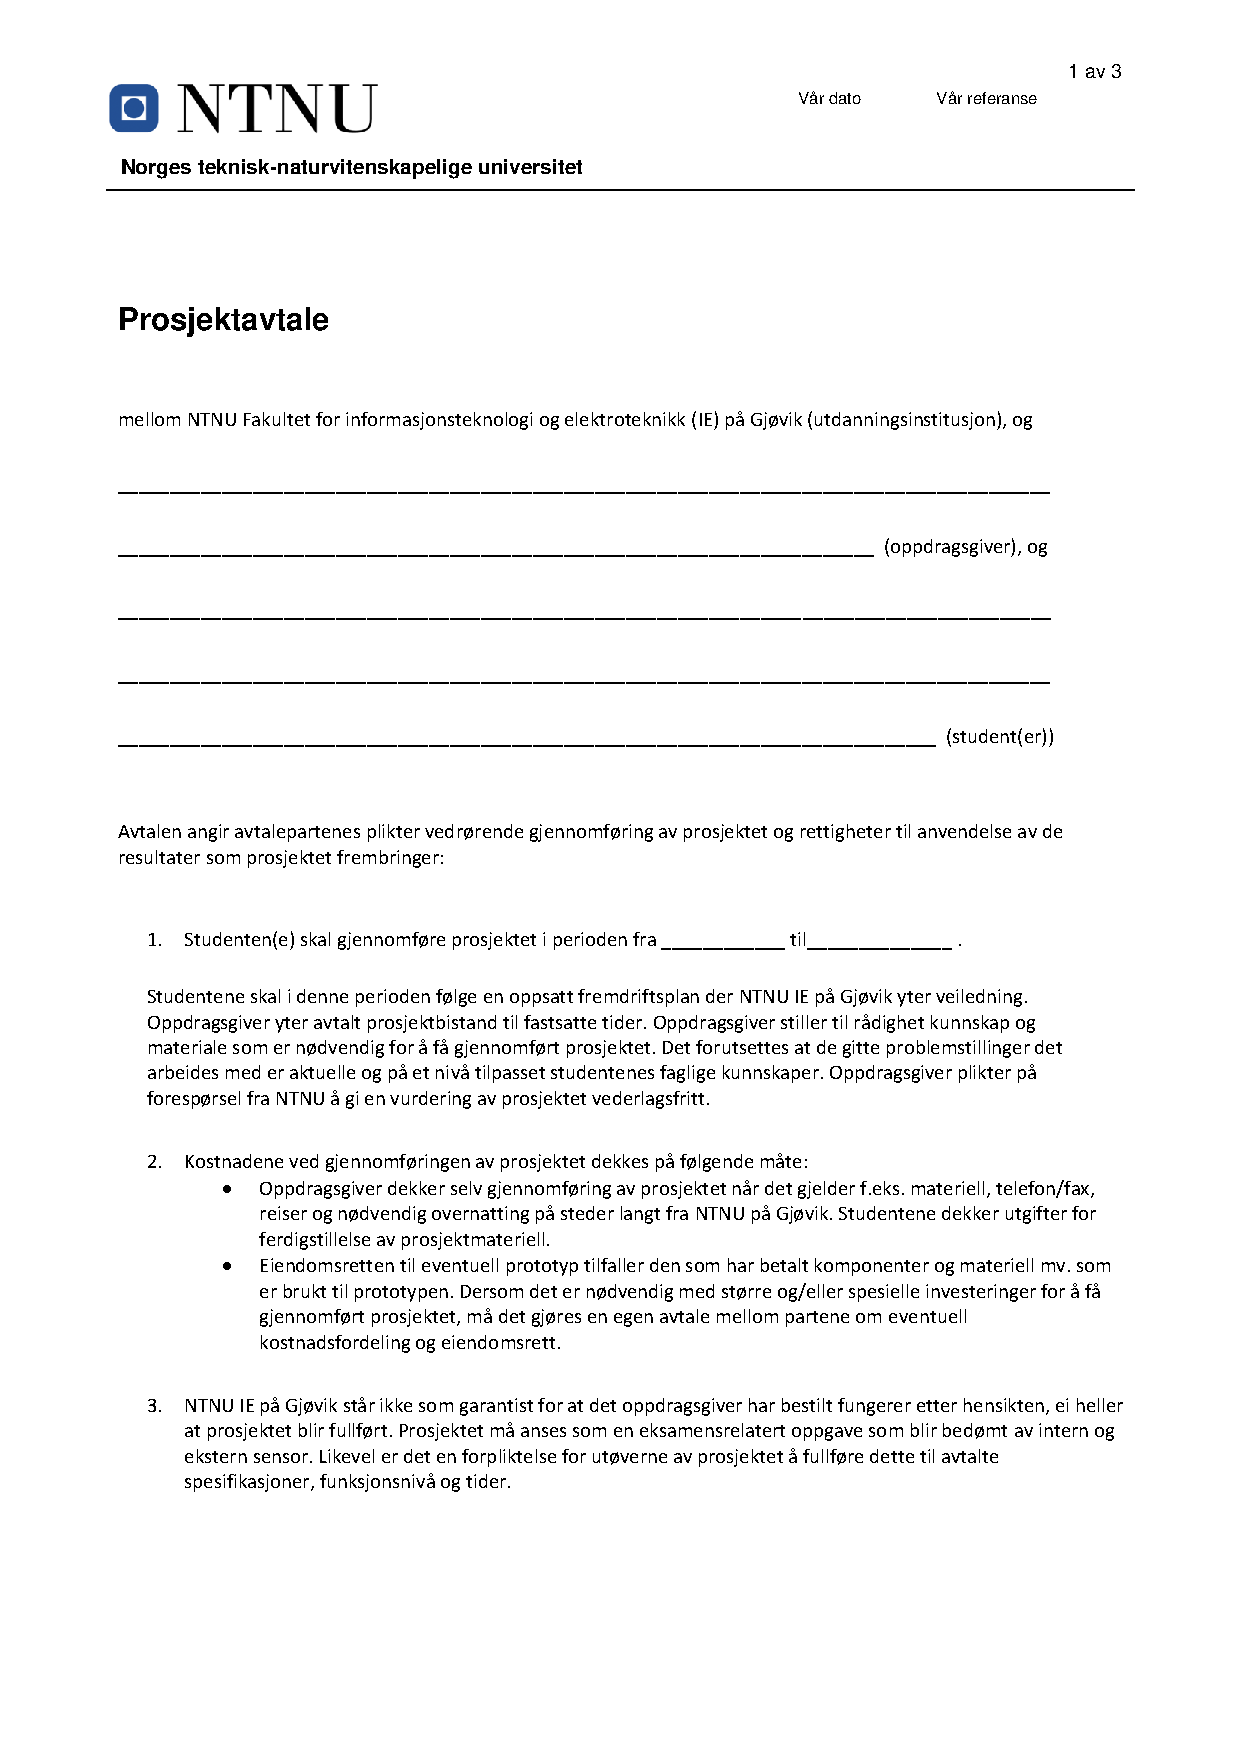
\includepdf[pages=-]{appendices/assets/NTNUProsjektavtale.pdf}

\end{document}
